% SPDX-License-Identifier: CC-BY-SA-4.0
% Author: Matthieu Perrin

\begingroup

\part{Introduction}
 
 
\section{Objectifs}
 
%\subsection{Notion de langages formels}
%% SPDX-License-Identifier: CC-BY-SA-4.0
% Author: Matthieu Perrin
% Part: 
% Section: 
% Sub-section: 
% Frame: 

\begingroup


\begin{frame}{Objet d'étude}
  On s'intéresse aux langages \alert{formels} :
  \begin{itemize}
  \item modélisation mathématique (abstraite) de la notion de langage
  \end{itemize}
  
  \begin{block}{Définition -- Alphabet et symbole}
    Un \structure{alphabet} est un \alert{ensemble fini non vide}\\
    Ses éléments sont appelés \structure{symboles}
  \end{block}
  \begin{block}{Définition -- Mot}
    Un \structure{mot} sur un alphabet $\Sigma$ est une \alert{suite finie de symboles} de $\Sigma$
  \end{block}
  \begin{block}{Définition -- Langage}
    Un \structure{langage} sur un alphabet $\Sigma$ est un \alert{ensemble de mots} sur $\Sigma$
  \end{block}
  \begin{alertblock}{Remarque}
    La \alert{théorie des langages formels} s'ancre dans la \alert{théorie des ensembles}
  \end{alertblock}
\end{frame}

\endgroup

%% SPDX-License-Identifier: CC-BY-SA-4.0
% Author: Matthieu Perrin
% Part: 
% Section: 
% Sub-section: 
% Frame: 

\begingroup

\begin{frame}{Exemple : un langage naturel}

  \begin{block}{Lexique français}
    \begin{description}
    \item[Langage :] L'ensemble des mots du \structure{dictionnaire}
    \item[Alphabet :] $\Sigma_{LF} \eqdef \{\text{`a'}, ...,  \text{`z'}, \text{`à'}, ..., \text{`ü'}, \text{`ç'}, \text{`-'}, \text{`\textquotesingle'}\}$
    \item[Mots :] $\{\text{``a''}, \text{``à''}, \text{``abaissement''}, ..., \text{``zut''}, \text{``zygomatique''}, \text{``zygote''}\}$
    \end{description}
  \end{block}
  
  \pause
  \begin{block}{Syntaxe française}
    \begin{description}
    \item[Langage :] L'ensemble des phrases/textes \structure{grammaticalement} correctes
    \item[Alphabet :] $\Sigma_{SF} \eqdef \Sigma_{LF} \cup \{\text{`A'}, ..., \text{`Z'}, \text{`~'}, \text{`.'}, \text{`?'}, ...\}$
    \item[Mots :] $\{\text{``A beau mentir qui vient de loin''}, \text{``À bon chat, bon rat''}, ...\}$
    \end{description}
  \end{block}
  
  \pause
  \begin{alertblock}{Sémantique française}
    \begin{itemize}
    \item \alert{Attention :} `a' (lettre) $\neq$ ``a'' (mot) $\neq$ a (conjugaison de avoir)
    \item On s'intéressera peu à la sémantique dans ce cours
    \item On n'écrira généralement pas les guillemets
    \end{itemize}
  \end{alertblock}

\end{frame}

\endgroup

%% SPDX-License-Identifier: CC-BY-SA-4.0
% Author: Matthieu Perrin
% Part: 
% Section: 
% Sub-section: 
% Frame: 

\begingroup


\begin{frame}{Exemple : un langage de programmation}
  C++ a également un lexique et une syntaxe.
  \begin{block}{Lexique du C++}
    \begin{description}
    \item[Mots-clés] \lstinline{if}, \lstinline{while}, \lstinline{class}, \lstinline{typedef}, ...
    \item[Identifiants :] \lstinline{x}, \lstinline{age}, \lstinline{number\_of\_participants}
    \item[Constantes :] \lstinline{5}, \lstinline{-3.14}, \lstinline{0x3A88C6}, \lstinline{'\\t'}, \lstinline{"Hello world"}, ...
    \item[Symboles :] \lstinline{(}, \lstinline{)}, \lstinline{\;}, \lstinline{+}, ...
    \end{description}
    \alert{Remarque :} le lexique du C++ est infini... mais ``simple'' $\rightarrow$ \structure{langage rationnel}
  \end{block}
  
  \begin{block}{Syntaxe du C++}
    \begin{description}
    \item[Expressions :] \lstinline{(-b + std::sqrt(b * b - 4 * a * c)) / (2 * a)}
    \item[Structures de contrôle :] \lstinline{if(condition()) \{p\_true()\;\} else \{p\_false()\;\}}
    \item[Structures de données :] \lstinline{struct pair \{int x\; int y;\}\;}
    \end{description}
    \alert{Remarque :} syntaxe définie récursivement $\rightarrow$ \structure{langage algébrique}
  \end{block}
\end{frame}
\endgroup

%% SPDX-License-Identifier: CC-BY-SA-4.0
% Author: Matthieu Perrin
% Part: 
% Section: 
% Sub-section: 
% Frame: 

\begingroup

\tikzset{
  compstep/.style ={draw, rectangle, rounded corners, fill=#1!20, text width=30mm, text height=2mm, align=center, rotate=90, font={\footnotesize}},
  compstep2/.style={draw, rectangle, rounded corners, fill=structure!20, minimum width=2cm, minimum height=1.1cm, align=center},
  compback/.style ={draw, rectangle, rounded corners, fill=example!15},
  complabel/.style={anchor=north, align=center, minimum height=3mm, inner sep=0pt, outer sep=0pt, above=1mm of #1, font={\small}},
  comppath/.style ={-latex, font={\scriptsize}},
}

\begin{frame}{Architecture d'un compilateur}
    \on[top]{
      \begin{tikzpicture}[x=8mm,anchor=base]
        \node                     (start)                          {};
        \node[compstep=structure] (front1) at ($(start)  + (2.0,0)$) {Analyse lexicale};
        \node[compstep=structure] (front2) at ($(front1) + (1.0,0)$) {Analyse syntaxique};
        \node[compstep=white    ] (front3) at ($(front2) + (1.0,0)$) {Analyse contextuelle};
        \node[compstep=white    ] (front4) at ($(front3) + (1.0,0)$) {Élaboration};
        \node[compstep=white    ] (optim1) at ($(front4) + (1.5,0)$) {Optimisation $1$};
        \node[compstep=white    ] (optimn) at ($(optim1) + (1.5,0)$) {Optimisation $n$};
        \node[compstep=white    ] (back1)  at ($(optimn) + (1.5,0)$) {Sélection d'instructions};
        \node[compstep=white    ] (back2)  at ($(back1)  + (1.0,0)$) {Ordonnancement};
        \node[compstep=white    ] (back3)  at ($(back2)  + (1.0,0)$) {Allocation de registres};
        \node[compstep=white    ] (back4)  at ($(back3)  + (1.0,0)$) {Génération};
        \node                     (end)    at ($(back4)  + (2.0,0)$) {};
   
        \node[complabel=$.5*(front1.east)+.5*(front4.east)$] (front) {Front end};
        \node[complabel=$.5*(optim1.east)+.5*(optimn.east)$] (optim) {Optimiseur};
        \node[complabel=$.5*(back1.east)+.5*(back4.east)$  ] (back)  {Back end};
        
        \begin{pgfonlayer}{background}
          \node[compback, fit=(front1)(front4)(front)] {};
          \node[compback, fit=(optim1)(optimn)(optim)] {};
          \node[compback, fit=(back1)(back4)(back)   ] {};
        \end{pgfonlayer}
        
        \scriptsize
        \path[comppath] (start)   edge node[above]{Langage} node[below]{source} (front1);
        \path[comppath] (front1)  edge                                          (front2);
        \path[comppath] (front2)  edge                                          (front3);
        \path[comppath] (front3)  edge                                          (front4);
        \path[comppath] (front4)  edge                                          (optim1);
        \path[comppath] (optim1)  edge node[above]{...}                         (optimn);
        \path[comppath] (optimn)  edge                                          (back1);
        \path[comppath] (back1)   edge                                          (back2);
        \path[comppath] (back2)   edge                                          (back3);
        \path[comppath] (back3)   edge                                          (back4);
        \path[comppath] (back4)   edge node[above]{Langage} node[below]{cible}  (end);
      \end{tikzpicture}
    }
   
    \onBlock[bottom]{Objectifs du cours}{
      \begin{itemize}
      \item \vspace{-2mm} Comprendre comment un compilateur ``lit'' le code source
      \item Concevoir un interpréteur pour le langage algorithmique
      \end{itemize}
    }
   
    \on[y=-17mm]{
      \begin{tikzpicture}[x=5mm]
        \node            (start)   at (00, 0) {};
        \node[compstep2] (lexer)   at (05, 0) {Analyseur\\lexical\vspace{2mm}\\\textit{Lexer}};
        \node[compstep2] (parser)  at (14, 0) {Analyseur\\syntaxique\vspace{2mm}\\\textit{Parser}};
        \node            (end)     at (20, 0) {};
   
        \scriptsize
        \path[-latex] (start) edge
        node[above,align=center]{Langage\\ source}
        node[below, example]{$15+2 * x$}
        (lexer);
   
        \path[-latex] (lexer) edge
        node[above]{Chaîne de tokens}
        node[below, example]{$\textsc{int}~\textsc{plus}~\textsc{int}~\textsc{times}~\textsc{var}$}
        (parser);
        
        \path[-latex] (parser) edge
        node[above, align=center]{Arbre de la syntaxe\\abstraite (AST)}
        node[below, example]{
          \begin{tikzpicture}[tree, x=7mm,y=4mm]
            \tree    {$+$}{
              \tree  {$15$}{}
              \tree  {$*$}{
                \tree{$2$}{}
                \tree{$x$}{}
              }
            }
          \end{tikzpicture}
        }
        (end);
      \end{tikzpicture}
    }
\end{frame}

\endgroup

% 
%\subsection{Langages et problèmes de décision}
%% SPDX-License-Identifier: CC-BY-SA-4.0
% Author: Matthieu Perrin
% Part: 
% Section: 
% Sub-section: 
% Frame: 

\begingroup

\begin{frame}{Exemple : test de primalité}
  \begin{block}{Représentation décimale des nombres}
    Soit $\Sigma = \{\text{`0'}, \text{`1'}, \text{`2'}, ..., \text{`9'}\}$ l'ensemble des chiffres.
    
    Pour un entier $n \in \mathbb{N}$, on note \structure{$(n)_{10}$} sa représentation décimale. 
    
    \begin{description}
    \item[\alert{Attention :}] `3' (chiffre) $\neq$ ``3'' (représentation décimale) $\neq$ 3 (nombre)
    \end{description}
    
    \begin{itemize}
    \item $\mathcal{L}_{\mathbb{N}} = \{(n)_{10} | n \in \mathbb{N}\} = \{\text{``0''},\text{``1''},\text{``2''},\text{``3''}, \text{``4''}, \text{``5''}, ...\}$
    \item<2-> $\mathcal{L}_{\mathbb{P}} = \{(n)_{10} | n \in \mathbb{N} \land n \text{ est premier}\} = \{\text{``2''},\text{``3''},\text{``5''}, \text{``7''}, \text{``11''}, ...\}$
    \end{itemize}
  \end{block}
  
  \vspace{3mm} 
  
  \begin{exampleblock}{Exercice}
    \begin{description}
    \item[Question :] $\text{``1547''} \in \mathcal{L}_{\mathbb{N}}$ ?
    \item<2->[Question :] $\text{``1547''} \in \mathcal{L}_{\mathbb{P}}$ ?
    \item<3->[Indication :] $1547 = 7 \times 13 \times 17$ 
    \end{description}
  \end{exampleblock}
  
  \uncover<3->{
    \centering
    \alert{Pour savoir si $(n)_{10}\in \mathcal{L}_{\mathbb{P}}$, il faut et il suffit de savoir si $n$ est premier }
  }  
\end{frame}

\endgroup

%% SPDX-License-Identifier: CC-BY-SA-4.0
% Author: Matthieu Perrin
% Part: 
% Section: 
% Sub-section: 
% Frame: 

\begingroup

\begin{frame}{Problème binaire et problème de décision}
  
  Un \structure{problème binaire} est une question dont la réponse est \alert{oui} ou \alert{non} en fonction de ses \structure{entrées}.
  
  \begin{exampleblock}{Exemples}
    \vspace{-2mm}
    \begin{itemize}
    \item \example{Primalité :} un entier est-il premier ?  
    \item \example{Classification :} une image donnée contient-elle un chat ? 
    \item \example{Base de données :} une requête donnée retourne-t-elle des résultats ?  
    \item \example{Sudoku :} une grille donnée peut-elle être remplie ? 
    \item \example{SAT :} une formule en forme normale conjonctive est-elle satisfiable ? 
    \item \example{Preuve :} étant donné un énoncé de théorème, peut-on le démontrer ? 
    \item \example{Décision :} étant donnés un mot $u$ et un langage $L$, a-t-on $u\in L$ ? 
    \end{itemize}
  \end{exampleblock}
  \pause
  \begin{alertblock}{Observations}
    \vspace{-2mm}
    \begin{itemize}
    \item En informatique, les entrées sont toujours des suites de 0 et de 1
    \item \alert{Les langages sont une métaphore des problèmes binaires}
    \item On peut généraliser aux problèmes qui ne sont pas binaires
    \end{itemize}
  \end{alertblock}
  
\end{frame}

\endgroup

%% SPDX-License-Identifier: CC-BY-SA-4.0
% Author: Matthieu Perrin
% Part: 
% Section: 
% Sub-section: 
% Frame: 

\begingroup


\begin{frame}{Exemple : représentation d'un nombre réel}

  \begin{block}{Langage représentant le calcul des décimales de $\pi$}
    On étend la notation \structure{$(n)_{10}$} aux nombres $n$ décimaux. 
    \begin{itemize}
    \item Pour $x\in \mathbb{R}$, on note $\alert{\mathcal{L}_{x}}$ le langage des troncatures de $x$
      $$\alert{\mathcal{L}_{x} \eqdef \left\{\left(\frac{\left\lfloor 10^n x \right\rfloor}{10^n} \right)_{10} \Big| n \in \mathbb{N}\right\}}$$
    \item Par exemple, $\example{\mathcal{L}_{\pi} = \left\{\text{``3''}, \text{``3.1''}, \text{``3.14''}, \text{``3.141''}, \text{``3.1415''}, ...   \right\}}$
    \end{itemize}
  \end{block}

  \pause

  \begin{alertblock}{Remarques}
    \begin{itemize}
    \item L'ensemble des langages est indénombrable
      \begin{itemize}
      \item Au moins autant de langages $\alert{\mathcal{L}_{x}}$ que de réel $\alert{x}$
      \end{itemize}
    \item Tout langage est dénombrable
      \begin{itemize}
      \item Par exemple, le langage des mots sur $\{1, 2\}$ est inclus dans $\alert{\mathcal{L}_{\mathbb{N}}}$
      \end{itemize}
    \item Aucun langage ne peut exprimer tous les langages 
      \begin{itemize}
      \item Même les langages de programmation $\rightarrow$ \alert{problèmes indécidables}
      \item Même le langage des mathématiques ~$\rightarrow$ \alert{problèmes indéfinissables}
      \end{itemize}
    \end{itemize}
  \end{alertblock}

\end{frame}

\endgroup

%% SPDX-License-Identifier: CC-BY-SA-4.0
% Author: Matthieu Perrin
% Part: 
% Section: 
% Sub-section: 
% Frame: 

\begingroup


\begin{frame}{Hiérarchie des langages}

  \tfBlock[top]{Formalismes de description d'un langage}{
    \begin{itemize}
    \item Comment représenter un langage \structure{infini} de façon \structure{finie} ?
    \item Il doit avoir une \alert{structure} interne
    \item La ``\structure{complexité}'' de sa structure entraine la ``\structure{difficulté}'' à le décider
    \end{itemize}
  }

  \tf[y=-17mm]{\footnotesize
    \begin{tikzpicture}
      \draw[structure, fill=structure!20] (12mm,12mm) ellipse(40mm and 21mm); \draw (12mm,30mm) node{définissable};
      \draw[structure, fill=structure!10] (10mm,10mm) ellipse(35mm and 18mm); \draw (10mm,25mm) node{récursivement énumérable};
      \draw[structure, fill=structure!20] (08mm,08mm) ellipse(30mm and 15mm); \draw (08mm,20mm) node{décidable};
      \draw[structure, fill=structure!10] (06mm,06mm) ellipse(25mm and 12mm); \draw (06mm,15mm) node{contextuel};
      \draw[structure, fill=structure!20] (04mm,04mm) ellipse(20mm and 09mm); \draw (04mm,10mm) node{algébrique};
      \draw[structure, fill=structure!10] (02mm,02mm) ellipse(15mm and 06mm); \draw (02mm,05mm) node{rationnel};
      \draw[structure, fill=structure!20] (00mm,00mm) ellipse(10mm and 03mm); \draw (00mm,00mm) node{fini};
    \end{tikzpicture}
  }
  
\end{frame}


\endgroup

% 
%\subsection{Automates}
%% SPDX-License-Identifier: CC-BY-SA-4.0
% Author: Matthieu Perrin
% Part: 
% Section: 
% Sub-section: 
% Frame: 

\begingroup

\begin{frame}{Et les automates ?}

  \on[text, top=-2mm]{
    \begin{description}
    \item[Langage :] abstraction d'un problème binaire
    \item[Automate :] abstraction d'une solution au problème binaire
      \begin{itemize}
      \item Modèle mathématique d'une structure algorithmique
      \item Différents types selon l'organisation de la mémoire
      \end{itemize}
    \end{description}
  }
 
  \onBlock<2->[y=10mm]{La hiérarchie de Chomsky}{}
 
  \on<2->[x=-15mm, y=-15mm]{\small
    \begin{tikzpicture}[2Darray]
      \arrayColumn[header=Langage,width=28mm]{
        \arrayLine[anchor=center,]{Récursivement\\ énumérable}
        \arrayLine[anchor=center,]{Contextuel}
        \arrayLine[structure]{Algébrique}
        \arrayLine[structure]{Rationnel}
      }
      \arrayColumn[header=Automate,width=28mm]{
        \arrayLine{Machine de Turing}
        \arrayLine{Automate\\linéairement borné}
        \arrayLine[structure]{Automate à pile\\non déterministe}
        \arrayLine[structure]{Automate fini}
      }
      \arrayColumn[header=Exemples,width=28mm]{
        \arrayLine{Primalité, \\Sudoku...}
        \arrayLine{Langues\\naturelles}
        \arrayLine[structure]{Langages de\\programmation}
        \arrayLine[structure]{Identifiants,\\ nombres...}
      }
    \end{tikzpicture}
  }
  
  \onImage<2->[x=45mm,y=-17mm]{%
    width=2.2cm,
    title={Noam Chomsky},
    license={{\href{https://creativecommons.org/licenses/by-sa/4.0/}{CC BY-SA}} (\ccbysa{} — 2017, \href{https://commons.wikimedia.org/wiki/File:Noam_Chomsky_portrait_2017_retouched.png}{Wikimedia})},
    img={Chomsky.jpg}
  }
  
\end{frame}

\endgroup

%% SPDX-License-Identifier: CC-BY-SA-4.0
% Author: Matthieu Perrin
% Part: 
% Section: 
% Sub-section: 
% Frame: 

\begingroup

\tikzset{
  compstep/.style ={draw, rectangle, rounded corners, fill=#1!20, text width=30mm, text height=2mm, align=center, rotate=90, font={\footnotesize}},
  compstep2/.style={draw, rectangle, rounded corners, fill=structure!20, minimum width=2cm, minimum height=1.1cm, align=center},
  compback/.style ={draw, rectangle, rounded corners, fill=example!15},
  complabel/.style={anchor=north, align=center, minimum height=3mm, inner sep=0pt, outer sep=0pt, above=1mm of #1, font={\small}},
  comppath/.style ={-latex, font={\scriptsize}},
}

\begin{frame}{Architecture d'un compilateur}
    \on[top]{
      \begin{tikzpicture}[x=8mm,anchor=base]
        \node                     (start)                          {};
        \node[compstep=structure] (front1) at ($(start)  + (2.0,0)$) {Analyse lexicale};
        \node[compstep=structure] (front2) at ($(front1) + (1.0,0)$) {Analyse syntaxique};
        \node[compstep=white    ] (front3) at ($(front2) + (1.0,0)$) {Analyse contextuelle};
        \node[compstep=white    ] (front4) at ($(front3) + (1.0,0)$) {Élaboration};
        \node[compstep=white    ] (optim1) at ($(front4) + (1.5,0)$) {Optimisation $1$};
        \node[compstep=white    ] (optimn) at ($(optim1) + (1.5,0)$) {Optimisation $n$};
        \node[compstep=white    ] (back1)  at ($(optimn) + (1.5,0)$) {Sélection d'instructions};
        \node[compstep=white    ] (back2)  at ($(back1)  + (1.0,0)$) {Ordonnancement};
        \node[compstep=white    ] (back3)  at ($(back2)  + (1.0,0)$) {Allocation de registres};
        \node[compstep=white    ] (back4)  at ($(back3)  + (1.0,0)$) {Génération};
        \node                     (end)    at ($(back4)  + (2.0,0)$) {};
   
        \node[complabel=$.5*(front1.east)+.5*(front4.east)$] (front) {Front end};
        \node[complabel=$.5*(optim1.east)+.5*(optimn.east)$] (optim) {Optimiseur};
        \node[complabel=$.5*(back1.east)+.5*(back4.east)$  ] (back)  {Back end};
        
        \begin{pgfonlayer}{background}
          \node[compback, fit=(front1)(front4)(front)] {};
          \node[compback, fit=(optim1)(optimn)(optim)] {};
          \node[compback, fit=(back1)(back4)(back)   ] {};
        \end{pgfonlayer}
        
        \scriptsize
        \path[comppath] (start)   edge node[above]{Langage} node[below]{source} (front1);
        \path[comppath] (front1)  edge                                          (front2);
        \path[comppath] (front2)  edge                                          (front3);
        \path[comppath] (front3)  edge                                          (front4);
        \path[comppath] (front4)  edge                                          (optim1);
        \path[comppath] (optim1)  edge node[above]{...}                         (optimn);
        \path[comppath] (optimn)  edge                                          (back1);
        \path[comppath] (back1)   edge                                          (back2);
        \path[comppath] (back2)   edge                                          (back3);
        \path[comppath] (back3)   edge                                          (back4);
        \path[comppath] (back4)   edge node[above]{Langage} node[below]{cible}  (end);
      \end{tikzpicture}
    }
   
    \onBlock[bottom]{Objectifs du cours}{
      \begin{itemize}
      \item \vspace{-2mm} Comprendre comment un compilateur ``lit'' le code source
      \item Concevoir un interpréteur pour le langage algorithmique
      \end{itemize}
    }
   
    \on[y=-17mm]{
      \begin{tikzpicture}[x=5mm]
        \node            (start)   at (00, 0) {};
        \node[compstep2] (lexer)   at (05, 0) {Analyseur\\lexical\vspace{2mm}\\\textit{Lexer}};
        \node[compstep2] (parser)  at (14, 0) {Analyseur\\syntaxique\vspace{2mm}\\\textit{Parser}};
        \node            (end)     at (20, 0) {};
   
        \scriptsize
        \path[-latex] (start) edge
        node[above,align=center]{Langage\\ source}
        node[below, example]{$15+2 * x$}
        (lexer);
   
        \path[-latex] (lexer) edge
        node[above]{Chaîne de tokens}
        node[below, example]{$\textsc{int}~\textsc{plus}~\textsc{int}~\textsc{times}~\textsc{var}$}
        (parser);
        
        \path[-latex] (parser) edge
        node[above, align=center]{Arbre de la syntaxe\\abstraite (AST)}
        node[below, example]{
          \begin{tikzpicture}[tree, x=7mm,y=4mm]
            \tree    {$+$}{
              \tree  {$15$}{}
              \tree  {$*$}{
                \tree{$2$}{}
                \tree{$x$}{}
              }
            }
          \end{tikzpicture}
        }
        (end);
      \end{tikzpicture}
    }
\end{frame}

\endgroup

% 
%\subsection{Généralités} 
%% SPDX-License-Identifier: CC-BY-SA-4.0
% Author: Matthieu Perrin
% Part: 
% Section: 
% Sub-section: 
% Frame: 

\begingroup

\begin{frame}{Généralités}
  
  \vspace{-1mm}
  \begin{block}{Prérequis}
    \begin{description}[Mathématiques :]
    \item[Mathématiques :]\vspace{-1mm} logique, théorie des ensembles
    \item[Informatique :] algorithmique, programmation impérative 
    \end{description}
  \end{block}

  \vspace{-1mm}
  \begin{block}{Objectifs théoriques}
    \begin{itemize}
    \item Comprendre les fondements mathématiques de l'informatique théorique
      \begin{itemize}
      \item Structures de mots et de langages
      \item Notion de non-déterminisme
      \item Frontières entre types de langages
      \end{itemize}
    \item Comprendre le fonctionnement de la partie avant des compilateurs
      \begin{description}[Analyse syntaxique :]
      \item[Analyse lexicale :] théorie des automates finis
      \item[Analyse syntaxique :] théorie des automates à pile 
      \end{description}
    \end{itemize}
  \end{block}

  \vspace{-1mm}
  \begin{block}{Objectifs pratiques}
    \begin{itemize}
    \item Créer un interpréteur en Java pour le langage d'algorithmique 
      \begin{itemize}
      \item JFlex et expressions rationnelles
      \item CUP et grammaires algébriques
      \end{itemize}
    \end{itemize}
  \end{block}

\end{frame}

\endgroup

%% SPDX-License-Identifier: CC-BY-SA-4.0
% Author: Matthieu Perrin
% Part: 
% Section: 
% Sub-section: 
% Frame: 

\begingroup

\begin{frame}{Bibliographie}
  \begin{block}{Livres}
    \footnotesize
    \begin{itemize}
    \item K. D. Cooper \& L. Torczon. \textit{\textbf{Engineering a compiler} -- $2^\text{nd}$ Ed.}, Morgan Kaufmann 2013
    \item A. Aho, R. Sethi \& J. Ullman. \textit{Compilateurs : principes, techniques et outils}, InterEditions, 1991. Voir aussi la seconde édition en anglais.
    \item P. Wolper. \textit{\textbf{Introduction à la calculabilité} -- $3^\text{nd}$ Ed.}, Dunod 2006
    \item O. Carton. \textit{Langages Formels -- Calculabilité et complexité}, Vuibert 2008
    \item J.-M. Autebert, \textit{Théorie des langages et des automates}, Masson 1994
    \item J.-M. Autebert, \textit{Langages algébriques}, Masson 1989
    \item P. Linz, \textit{Formal Languages and Automata}, Jones and Barnett Publishers, 2006.
    \item P. Séébold, \textit{Fondamentaux de la théorie des automates}, Ellipses, 2020.
    \end{itemize}
  \end{block}
  
  \begin{block}{Outil pédagogique}
    \footnotesize
    \begin{itemize}
    \item S. H. Rodger. \textit{JFLAP}. \url{http://www.jflap.org/} 
    \end{itemize}
  \end{block}
\end{frame}
\endgroup

% 
% 
% 
%\section{Mots et langages formels}
% 
%\subsection{Notion de mot}
%% SPDX-License-Identifier: CC-BY-SA-4.0
% Author: Matthieu Perrin
% Part: 
% Section: 
% Sub-section: 
% Frame: 

\begingroup

\begin{frame}{Alphabet}
  Soit $n\in \mathbb{N}$. On note $\alert{\llbracket n\rrbracket \eqdef \{x\in \mathbb{N} \,|\, 1 \le x \le n\} = \{1, ..., n\}}$.
  
  \begin{block}{Définition -- alphabet}
    Soit $E$ un ensemble.
    \begin{itemize}
    \item On dit que $E$ est \structure{fini} s'il existe $n\in \mathbb{N}$ et une bijection de $\llbracket n\rrbracket$ dans $E$. 
    \item Si un tel $n$ existe, il est unique. 
    \item $n$ est appelé le \structure{cardinal} de $E$, noté \alert{$|E|$}.
    \item Un \alert{ensemble fini non-vide} est appelé un \structure{alphabet}. 
    \end{itemize}
  \end{block}

  \begin{exampleblock}{Exemple}
    $\{a, b, c\}$ est un alphabet de cardinal 3, d'après la bijection suivante :

    $$
    \left\{\begin{array}{ccl}
    \llbracket 3\rrbracket &\rightarrow& \{a, b, c\}\\
    1 &\mapsto& a\\ 
    2 &\mapsto& b\\ 
    3 &\mapsto& c\\ 
    \end{array}\right.
    $$
  \end{exampleblock}
\end{frame}
\endgroup

%% SPDX-License-Identifier: CC-BY-SA-4.0
% Author: Matthieu Perrin
% Part: 
% Section: 
% Sub-section: 
% Frame: 

\begingroup

\begin{frame}{Mot}

  Soit $\Sigma$ un alphabet et $n\in \mathbb{N}$.
  \begin{itemize}
  \item Un \structure{mot} de longueur $n$ sur $\Sigma$ est une \alert{fonction de $\llbracket n\rrbracket$ dans $\Sigma$}.
  \item L'ensemble des mots de longueur $n$ sur $\Sigma$ est \alert{$\Sigma^n = \mathscr{F}\left(\llbracket n\rrbracket, \Sigma\right)$}.
  \item L'ensemble des mots sur $\Sigma$, noté \structure{$\Sigma^\star$}, est :
    $$\alert{\displaystyle \Sigma^\star \eqdef \bigcup_{n\in \mathbb{N}} \Sigma^n = \Sigma^0 \cup \Sigma^1 \cup \Sigma^2 \cup ...}$$
  \item L'ensemble des mots \structure{non-vides} sur $\Sigma$ est
    $\alert{\Sigma^+ \eqdef \bigcup_{n \neq 0 } \Sigma^n}$
  \end{itemize}

  \begin{exampleblock}{Exemples}
    Soit $\Sigma = \{a, b, ..., z\}$

    \begin{minipage}[t]{.5\textwidth}
      \begin{itemize}
      \item $\varepsilon = \left\{\begin{array}{ccc}
        \llbracket 0\rrbracket & \rightarrow & \Sigma\\
        x & \mapsto & \_
      \end{array}\right. \in \Sigma^0$
      \item $\text{``a''} = \left\{\begin{array}{ccc}
        \llbracket 1\rrbracket & \rightarrow & \Sigma\\
        x & \mapsto & \text{`a'}
      \end{array}\right. \in \Sigma^1$
      \end{itemize}
    \end{minipage}%
    \begin{minipage}[t]{.5\textwidth}
      \begin{itemize}
      \item $\text{``bon''} = \left\{\begin{array}{ccc}
        \llbracket 3\rrbracket& \rightarrow & \Sigma\\
        1 & \mapsto & \text{`b'}\\
        2 & \mapsto & \text{`o'}\\
        3 & \mapsto & \text{`n'}\\
      \end{array}\right. \in \Sigma^3$
      \end{itemize}
    \end{minipage}%
    \begin{itemize}
    \item Par abus de notation, on fera l'amalgame entre $\Sigma$ et $\Sigma^1$. 
    \end{itemize}
  \end{exampleblock}

\end{frame}

\endgroup

%% SPDX-License-Identifier: CC-BY-SA-4.0
% Author: Matthieu Perrin
% Part: 
% Section: 
% Sub-section: 
% Frame: 

\begingroup

\begin{frame}{Longueur et occurrences}
  Soient $\Sigma$ un alphabet, $a\in\Sigma$, $u\in \Sigma^\star$ et $i\in \left\llbracket |u|\right\rrbracket$.
  \begin{itemize}
  \item La \structure{longueur} de $u$, notée $\alert{|u|}$, est l'unique $n$ tel que $u\in \Sigma^n$
  \item On note \alert{$u[i] = u(i)$} le $i^\text{ème}$ caractère de $u$
  \item Une \structure{occurrence de $a$ dans $u$} est un entier $i\in \left\llbracket |u|\right\rrbracket$ tel que $u[i]=a$
  \item Le nombre d'occurrences de $a$ dans $u$ est noté $\alert{|u|_a}$
  \end{itemize}

  \begin{exampleblock}{Exemples}
    \begin{itemize}
    \item $|\text{``bon''}| = 3$
    \item $\forall x\in \Sigma^\star, |x| = 0 \Leftrightarrow x = \varepsilon$ car $\Sigma^0 = \{\varepsilon\}$
    \item 2 et 4 sont les deux occurrences de $\text{`a'}$ dans $\text{``banane''}$
    \item $|\text{``bon''}|_{\text{`o'}} = 1$
    \end{itemize}
  \end{exampleblock}
\end{frame}

\endgroup

%% SPDX-License-Identifier: CC-BY-SA-4.0
% Author: Matthieu Perrin
% Part: 
% Section: 
% Sub-section: 
% Frame: 

\begingroup

\begin{frame}{Concaténation}

  \tfBlock[top=-5mm]{Définition -- Concaténation de deux mots}{
    Soient $\Sigma$ un alphabet, $u, v \in \Sigma^\star$, et $n\in \mathbb{N}$.

    \begin{itemize}
    \item La \structure{concaténation} de $u$ et $v$, notée \structure{$u \cdot v$} (ou \structure{$uv$}), est le mot
      de longueur $|u| + |v| $ dont les premiers symboles forment $u$ et les derniers forment $v$
      $$\alert{
        u \cdot v  \quad\eqdef\quad  \left\{\begin{array}{@{}r@{~}c@{~}ll@{}}
        \llbracket |u| + |v| \rrbracket& \rightarrow & \Sigma\\
         i   & \mapsto & u_i & \text{pour } i \in \llbracket |u| \rrbracket \\
        |u| + j & \mapsto & v_j & \text{pour } j \in \llbracket |v| \rrbracket
        \end{array}\right.
        \quad=\quad u_1 \cdots u_{|u|} \cdot v_1 \cdots v_{|v|}
      }$$
    \item La \structure{puissance $n$ du mot $x$} est le mot \alert{$x^n = x\cdots x$} (répété $n$ fois)
      $$\alert{u^0 \eqdef \varepsilon} \quad \text{ et } \quad \alert{u^{n+1} \eqdef u \cdot u^n}$$
    \end{itemize}
  }

  \tfExampleBlock[bottom]{Exemple}{\small\vspace{-7mm}
    $$\text{``bon''} \cdot \text{``jour''} = \left\{
    \begin{array}{@{~}r@{~~}c@{~~}l@{~~}c@{~~}c@{~}}
    \llbracket 3 + 4 \rrbracket & \rightarrow & \Sigma\\
    1 & \mapsto & \text{``bon''}_{1}  & = &\text{`b'}\\
    2 & \mapsto & \text{``bon''}_{2}  & = &\text{`o'}\\
    3 & \mapsto & \text{``bon''}_{3}  & = &\text{`n'}\\
    3+1 & \mapsto & \text{``jour''}_{1} & = &\text{`j'}\\
    3+2 & \mapsto & \text{``jour''}_{2} & = &\text{`o'}\\
    3+3 & \mapsto & \text{``jour''}_{3} & = &\text{`u'}\\
    3+4 & \mapsto & \text{``jour''}_{4} & = &\text{`r'}\\
    \end{array}
    \right. = \text{``bonjour''}$$
  }

\end{frame}

\endgroup

%% SPDX-License-Identifier: CC-BY-SA-4.0
% Author: Matthieu Perrin
% Part: 
% Section: 
% Sub-section: 
% Frame: 

\begingroup



\begin{frame}{Structure de monoïde}
  Soit $\Sigma$ un alphabet. 
  
  \begin{block}{Propriétés de la concaténation}
  \begin{description}
  \item[Associativité :] $\forall u, v, w \in \Sigma^\star, \alert{(u\cdot v)\cdot w = u\cdot (v\cdot w)}$
    \begin{itemize}
    \item On notera $\structure{u\cdot v\cdot w}$
    \end{itemize}
  \item[Neutralité :] $\forall u \in \Sigma^\star, \alert{\varepsilon \cdot u = u = u \cdot \varepsilon}$
  \item[Simplifiabilité :] $\forall u, v, w \in \Sigma^\star,$
    \begin{description}
    \item[À gauche :] $\alert{u \cdot v = u \cdot w \Rightarrow v=w}$
    \item[À droite :] $\alert{v \cdot u = w \cdot u \Rightarrow v=w}$
    \end{description}
  \item[Non-commutativité :] $ \exists u,v \in \Sigma^\star, \alert{u\cdot v \neq v\cdot u}$
  \end{description}
  \end{block}

  \begin{block}{Remarque}
    Un \structure{monoïde} est un ensemble muni d'une loi de composition interne associative, et d'un élément neutre. \\
    Le monoïde \structure{$\langle \Sigma^\star, \cdot , \varepsilon \rangle$} est appelé \alert{monoïde libre engendré par $\Sigma$}.
  \end{block}
\end{frame}


\endgroup

%% SPDX-License-Identifier: CC-BY-SA-4.0
% Author: Matthieu Perrin
% Part: 
% Section: 
% Sub-section: 
% Frame: 

\begingroup

\begin{frame}{Décomposition}
  Soient $\Sigma$ un alphabet, $u, v \in \Sigma^\star$.

  \begin{block}{Théorème -- Décomposition}
    Tout mot $u\in \Sigma^\star$ se décompose de façon unique en $u_1\cdot u_2 \cdots u_{|u|}$,
    où $\forall i \in \llbracket |u| \rrbracket, u_i \in \Sigma^1$.
  \end{block}
  
  \begin{block}{Définitions -- Facteur, préfixe, suffixe}
    \begin{itemize}
    \item\vspace{-2mm}  $v$ est un \structure{facteur} \phantom{propr}\,\,\, de $u$ si \alert{$\exists x, y           \in \Sigma^\star\;, u = x \cdot v \cdot y$}
    \item\vspace{-.5mm} $v$ est un \structure{préfixe} \phantom{propre}    de $u$ si \alert{$\exists y\phantom{, x} \in \Sigma^\star\;, u = \phantom {w \cdot }\; v \cdot y$}
    \item\vspace{-.5mm} $v$ est un \structure{préfixe propre}              de $u$ si \alert{$\exists y\phantom{, x} \in \Sigma^+,      u = \phantom{ w \cdot }\; v \cdot y$}
    \item\vspace{-.5mm} $v$ est un \structure{suffixe} \phantom{propre}\,    de $u$ si \alert{$\exists x\phantom{, y} \in \Sigma^\star\;, u = x \cdot v$}
    \item\vspace{-.5mm} $v$ est un \structure{suffixe propre}\,              de $u$ si \alert{$\exists x\phantom{, y} \in \Sigma^+,      u = x \cdot v$}
    \item\vspace{-.5mm} L'ensemble des préfixes de $u$ est noté $\mathit{Pref}(u)$. 
    \item\vspace{-.5mm} L'ensemble des préfixes propres de $u$ est noté $\mathit{PrefProp}(u)$. 
    \item\vspace{-.5mm} L'ensemble des suffixes de $u$ est noté $\mathit{Suff}(u)$. 
    \item\vspace{-.5mm} L'ensemble des suffixes propres de $u$ est noté $\mathit{SuffProp}(u)$. 
    \end{itemize}
  \end{block}
\end{frame}

\endgroup

%% SPDX-License-Identifier: CC-BY-SA-4.0
% Author: Matthieu Perrin
% Part: 
% Section: 
% Sub-section: 
% Frame: 

\begingroup

\begin{frame}{Relation d'ordre}
  \small 
  Soit $\bowtie$ une relation binaire homogène sur un ensemble $E$.

  \begin{block}{Définition -- Relation d'ordre}
    $\bowtie$ est une \structure{relation d'ordre} si elle est \alert{réflexive}, \alert{transitive} et \alert{antisymétrique}.
  \end{block}
  \begin{exampleblock}{Exemple}
    Soit $E$ un ensemble. 
    Montrons que $\subseteq$ est une relation d'ordre sur $\mathscr{P}(E)$.
    \begin{description}
    \item[Réflexivité]  Montrons que \alert{$\forall A\in \mathscr{P}(E), A\subseteq A$}
      \begin{itemize}
      \item Soit \structure{$A \in \mathscr{P}(E)$}. Montrons que $\alert{A\subseteq A}$.
      \item Soit $x\in A$. On a $x\in A$.
      \end{itemize}
    \item[Transitivité] Montrons que \alert{$\forall A, B, C \in \mathscr{P}(E), A \subseteq B \land B \subseteq C \Rightarrow A \subseteq C$}
      \begin{itemize}
      \item Soient $\structure{A, B, C \in \mathscr{P}(E)}$, tels que $\structure{A \subseteq B}$ et $\structure{B \subseteq C}$. 
      \item Soit $x \in A$. Donc $x\in B$, donc $x\in C$. 
      \end{itemize}
    \item[Antisymétrie] Montrons que \alert{$\forall A,B \in \mathscr{P}(E), A \subseteq B \land B \subseteq A \Rightarrow A=B$}
      \begin{itemize}
      \item Soient $\structure{A, B \in \mathscr{P}(E)}$, tels que $\structure{A \subseteq B}$ et $\structure{B \subseteq A}$. 
      \item Par double inclusion, on a $A=B$. 
      \end{itemize}
    \end{description}
  \end{exampleblock}
\end{frame}
\endgroup

% 
%\subsection{Notion de langage}
%% SPDX-License-Identifier: CC-BY-SA-4.0
% Author: Matthieu Perrin
% Part: 
% Section: 
% Sub-section: 
% Frame: 

\begingroup

\begin{frame}{Langages reconnaissables par un AFN}
  Soit $\Sigma$ un alphabet.
  \begin{block}{Définition -- Langage reconnaissable}
    Un langage $L$ sur $\Sigma$ est \structure{reconnaissable} s'il est reconnu par un AFN. 

    L'ensemble des langages reconnaissables sur $\Sigma$ est noté \alert{$\textsc{rec}_\Sigma$} :

    \vspace{-2mm}
    $$\alert{\textsc{rec}_\Sigma \eqdef \{ L \in \mathscr{P}(\Sigma^\star) | \exists A, L = \mathcal{L}(A)\}} $$

  \end{block}
  
  \vspace{-3mm}
  \begin{alertblock}{Théorème}
    Tout langage reconnaissable est rationnel : $\alert{\textsc{rec}_\Sigma \subseteq \textsc{rat}_\Sigma}$.
  \end{alertblock}

  \begin{center}
    \structure{Étant donné un AFN $A$, comment déterminer une expression rationnelle décrivant $\mathcal{L}(A)$ ?}
  \end{center}
  
  \vspace{-3mm}
  \begin{block}{Étapes}
    \begin{itemize}
    \item \vspace{-3mm} Langage droit d'un état
    \item Système d'équations rationnelles
    \item Lemme d'Arden
    \end{itemize}
  \end{block}
\end{frame}

\endgroup

%% SPDX-License-Identifier: CC-BY-SA-4.0
% Author: Matthieu Perrin
% Part: 
% Section: 
% Sub-section: 
% Frame: 

\begingroup

\begin{frame}{Opérations sur les langages}
  Soit $\Sigma$ un alphabet, et $L, M \in \mathscr{P}(\Sigma^\star)$ deux langages. 
  
  \begin{block}{Rappel -- Opérations ensemblistes}
    \begin{itemize}
    \item\vspace{-1mm} \structure{Union : } $\alert{L \cup M} \eqdef \{ x \in \Sigma^\star \,|\, x \in L \lor x \in M\}$
    \item\vspace{-1mm} \structure{Intersection : } $\alert{L \cap M} \eqdef \{ x \in \Sigma^\star \,|\, x \in L \land x \in M\}$
    \item\vspace{-1mm} \structure{Différence : } $\alert{L \setminus M} \eqdef \{ x \in \Sigma^\star \,|\, x \in L \land x \notin M\}$
    \item\vspace{-1mm} \structure{Complémentaire : } $\alert{\overline{L}} \eqdef \{ x \in \Sigma^\star \,|\, x \notin L\} = \Sigma^\star \setminus L$
    \end{itemize}
  \end{block}
  \begin{block}{Définition -- Concaténation des langages}
    \begin{itemize}
    \item\vspace{-.5mm} \structure{Concaténation : } $\alert{L \cdot M} \eqdef \{ x \cdot y \,|\, x \in L \land y \in M\}$ (parfois noté $LM$)
    \item \structure{Puissance : } $L^n = L\cdot L \cdots L$ ($L$ est répété $n$ fois) :
      \begin{itemize}
      \item\vspace{-.5mm} $\alert{L^0} \eqdef \{\varepsilon\}$
      \item\vspace{-.5mm} $\alert{L^{n+1}} \eqdef L^n \cdot L$
      \end{itemize}
    \item\vspace{-.5mm} \structure{Fermeture de Kleene : } $\alert{L^\star} \eqdef \bigcup_{i\in \mathbb{N}} L^i$
    \item\vspace{-.5mm} \structure{Fermeture positive : } $\alert{L^+} \eqdef \bigcup_{i>0} L^i = L^\star \cdot L = L \cdot L^\star$
    \end{itemize}
  \end{block}
\end{frame}

\endgroup

%% SPDX-License-Identifier: CC-BY-SA-4.0
% Author: Matthieu Perrin
% Part: 
% Section: 
% Sub-section: 
% Frame: 

\begingroup

\begin{frame}{Structure d'algèbre de Kleene}
  Soient $\Sigma$ un alphabet et $L, L_1, L_2, L_3 \in \mathscr{P}(\Sigma)$ des langages. 
 
  \begin{itemize}
  \item \textbf{Union} \hspace{\fill} $\langle \mathscr{P}(\Sigma), \cup, \emptyset \rangle$ est un monoïde commutatif
    \begin{description}
    \item[neutralité :] $\emptyset \cup L = L = L \cup \emptyset$ 
    \item[associativité :] $L_1 \cup (L_2 \cup L_3) = (L_1 \cup L_2) \cup L_3$
    \item[commutativité :] $L_1 \cup L_2 = L_2 \cup L_1$
    \item[idempotence :] $L \cup L = L$
    \end{description}
  \item \textbf{Concaténation} \hspace{\fill} $\langle \mathscr{P}(\Sigma), \cdot, \{\varepsilon\} \rangle$ est un monoïde
    \begin{description}
    \item[neutralité :] $\{\varepsilon\} \cdot L = L = L \cdot \{\varepsilon\}$
    \item[associativité :] $L_1 \cdot (L_2 \cdot L_3) = (L_1 \cdot L_2) \cdot L_3$
    \item[absorption :] $L \cdot \emptyset = \emptyset = \emptyset \cdot L$
    \end{description}
  \item \textbf{Mise à l'étoile} 
    \begin{description}
    \item[neutralité :] $\emptyset^\star = \{\varepsilon\}$
    \item[idempotence :] $L^{\star^\star} = L^\star$
    \end{description}
  \item \textbf{Intéraction entre opérateurs} 
    \begin{description}
    \item[distributivité :] $L_1 \cdot (L_2 \cup L_3) = (L_1\cdot L_2) \cup (L_1 \cdot L_3)$\\
      $(L_2 \cup L_3) \cdot L_1 = (L_2\cdot L_1) \cup (L_3 \cdot L_1)$
    \item[absorption :] $L \cup L^\star = L^\star = L^\star \cup L$
    \item[fermetures :] $L^\star = \{ \varepsilon \} \cup L^+$
    \end{description}
  \end{itemize}
\end{frame}


\endgroup

% 
% 
%\part{Analyse Lexicale}
% 
% 
%\section{Langages et expressions rationnels}
% 
%\subsection{Expressions rationnelles}
%% SPDX-License-Identifier: CC-BY-SA-4.0
% Author: Matthieu Perrin
% Part: 
% Section: 
% Sub-section: 
% Frame: 

\begingroup

\begin{frame}{introduction aux langages rationnels}
  \begin{block}{Définition}
    Les \structure{langages rationnels} (ou \emph{réguliers}) sont les langages définis par :
    \begin{itemize}
      \item des expressions rationnelles
      \item des automates finis
      \item des grammaires linéaires
      \item des équations de type $X = aX + b$, etc
    \end{itemize}
    Ils forment une classe notée $\alert{\textsc{rat}_\Sigma \subsetneq \mathcal{P}(\Sigma^\star)}$.
  \end{block}

  \begin{block}{Pourquoi s’y intéresser ?}
    \begin{itemize}
      \item Ils modélisent des motifs simples et décidables
      \item Ils sont utilisés dans les outils de traitement de texte et de code :
        \begin{itemize}
          \item remplacement automatique (éditeurs de texte, compilateurs)
          \item recherche dans un fichier (\texttt{grep})
          \item découpage lexical (\texttt{JFlex}, analyse lexicale)
          \item vérification de chaînes (\texttt{java.util.regex.Pattern})
        \end{itemize}
    \end{itemize}
  \end{block}
\end{frame}

\endgroup

%% SPDX-License-Identifier: CC-BY-SA-4.0
% Author: Matthieu Perrin
% Part: 
% Section: 
% Sub-section: 
% Frame: 

\begingroup

\begin{frame}{Exemple d'utilisation du lemme de pompage}
  
  \tfBlock[top=-5mm]{Montrer que $L \eqdef \{a^nb^nc^n \mid n\in \mathbb{N}\}$ n'est pas algébrique}{
    Soit $\Sigma \eqdef \{a, b, c\}$.%
    \only<2-|handout>{
      Si $L$ est algébrique, $L$ vérifie le lemme de pompage :

      \vspace{-4mm}
      $$
      \begin{array}{c}
        \structure{\exists N\in \mathbb{N}}, \alert{\forall u\in L, |u| \ge N} \Rightarrow (\structure{\exists v, w, x, y, z\in \Sigma^\star}, \\
        u = v \cdot w \cdot x\cdot y \cdot z \land w \cdot y\neq \varepsilon \land |w\cdot x\cdot y| \le N \land \alert{\forall i \in \mathbb{N}}, v\cdot w^i\cdot x\cdot y^i \cdot z \in L)
      \end{array}
      $$
      \vspace{-2mm}
      
      \structure{Soit $N$ donné par le lemme pompage}.
    }
    
    \only<3-|handout>{%
      \alert{Posons $u = a^N b^N c^N$. On a bien $u\in L$ et $|u| = 3N \ge N$}.\\
      \structure{Soit $v \cdot w \cdot x\cdot y \cdot z$ la décomposition de $u$ donnée par le lemme de pompage}. 
    }
  }
  
  \tf<4-|handout>[y=-10mm]{
    \begin{smArray}[width=4mm, height=3mm, name={$u=$}]
      \smCell[\smNone]{\alert{$a$}}      \smCoord{(a1)}
      \smCell[\smNone]{\alert{$\cdots$}}               
      \smCell[\smNone]{\alert{$a$}}      \smCoord{(an)}
      \smCell[\smNone]{\alert{$\cdot$}}               
      \smCell[\smNone]{\alert{$b$}}      \smCoord{(b1)}
      \smCell[\smNone]{\alert{$\cdots$}}               
      \smCell[\smNone]{\alert{$b$}}      \smCoord{(bn)}
      \smCell[\smNone]{\alert{$\cdot$}}               
      \smCell[\smNone]{\alert{$c$}}      \smCoord{(c1)}
      \smCell[\smNone]{\alert{$\cdots$}}               
      \smCell[\smNone]{\alert{$c$}}      \smCoord{(cn)}
      
      \draw [decorate, decoration={brace, amplitude=5pt}] ([xshift=1mm]a1.north west) -- ([xshift=-1mm]an.north east) node[midway,yshift=4mm]{$N$};
      \draw [decorate, decoration={brace, amplitude=5pt}] ([xshift=1mm]b1.north west) -- ([xshift=-1mm]bn.north east) node[midway,yshift=4mm]{$N$};
      \draw [decorate, decoration={brace, amplitude=5pt}] ([xshift=1mm]c1.north west) -- ([xshift=-1mm]cn.north east) node[midway,yshift=4mm]{$N$};

      \draw [decorate, decoration={brace, amplitude=5pt, mirror}] ([xshift=1mm]an.south west) -- ([xshift=-1mm]b1.south east) node[midway,yshift=-4mm]{$|wxy|\le N$};
      \draw [decorate, decoration={brace, amplitude=5pt, mirror}] ([xshift=1mm]bn.south west) -- ([xshift=-1mm]c1.south east) node[midway,yshift=-4mm]{$|wxy|\le N$};
    \end{smArray}       
  }

  \tf<5-|handout>[text, bottom=-1mm]{
    \begin{itemize}
    \item Comme $wy \neq \varepsilon$, $\alpha = wy[1] \in \Sigma$ est une lettre de $wy$.
    \item Comme $|wxy| \le N$, il existe $\beta \in \Sigma$ tel que $\beta$ n'est pas une lettre de $wy$. 
    \item \alert{Posons $i=2$}. $|v \cdot w^2 \cdot x\cdot  y^2\cdot   z|_\alpha > |v\cdot  w^2\cdot  x\cdot  y^2\cdot   z|_\beta$, donc $v\cdot  w^2\cdot  x\cdot  y^2\cdot   z\notin L$. 
    \end{itemize}
    Absurde ! Donc $L$ n'est pas algébrique. 
  }

  \tfExampleBlock<-4>[y=-25mm]{On sait}{}

  \tf<1>[y=-25mm, anchor=north, text]{
    \begin{itemize}
    \item $\begin{array}[t]{l}
      \alert{\forall L \in \textsc{alg}_\Sigma}, \structure{\exists N\in \mathbb{N}}, \forall u\in L, |u| \ge N \Rightarrow (\exists v, w, x, y, z\in \Sigma^\star, \\
      u = v w x y z \land w y\neq \varepsilon \land |wxy| \le N \land \forall i \in \mathbb{N}, v w^i x y^i z \in L)
    \end{array}$
    \end{itemize}
  }

  \tf<2-4>[y=-25mm, anchor=north, left=.35\textwidth]{
    \begin{itemize}
    \item $L \in \textsc{alg}_\Sigma$
    \item<3-> $v, w, x, y, z\in \Sigma^\star$
    \end{itemize}
  }
  
  \tf<2-4>[y=-25mm, anchor=north, width=.35\textwidth]{
    \begin{itemize}
    \item $N \in \mathbb{N}$
    \item<3-> $wy\neq \varepsilon$
    \end{itemize}
  }
  
  \tf<3-4>[y=-25mm, anchor=north, right=.35\textwidth]{
    \begin{itemize}
    \item $v \cdot w \cdot x \cdot y \cdot z = a^N b^N c^N$
    \item $\alert{|wxy| \le N}$
    \end{itemize}
  }
  
\end{frame}

\endgroup

%% SPDX-License-Identifier: CC-BY-SA-4.0
% Author: Matthieu Perrin
% Part: 
% Section: 
% Sub-section: 
% Frame: 

\begingroup

\begin{frame}{Construction des expressions rationnelles}
  
  Les expressions rationnelles sur un alphabet $\Sigma$ sont construites par induction
  
  \begin{description}[xxxxxxxxxxx]
  \item[$\emptyset$ :] représente le langage vide \alert{$\emptyset$}
  \item[$\varepsilon$ :] représente le langage neutre \alert{$\{\varepsilon\}$}
  \item[$a$ :] représente le langage \alert{$\{a\}$}, pour tout $a\in \Sigma$
  \item[$\mathit{reg}_1 \cdot \mathit{reg}_2$ :] représente le langage \alert{$\mathcal{L}(\mathit{reg}_1) \cdot \mathcal{L}(\mathit{reg}_2)$}
  \item[$\mathit{reg}_1 \mid \mathit{reg}_2$ :] représente le langage \alert{$\mathcal{L}(\mathit{reg}_1) \cup \mathcal{L}(\mathit{reg}_2)$}
  \item[$\mathit{reg}^\star$ :] représente le langage \alert{$\mathcal{L}(\mathit{reg})^\star$}
  \end{description}

  Où \structure{$\mathcal{L}(\mathit{reg})$} est le langage représenté par l'expression rationnelle $\mathit{reg}$

  \pause
  \begin{block}{Notations}
    \begin{itemize}
    \item L'opérateur \alert{$\cdot$} est le plus souvent \structure{omis}
    \item On utilise les règles de \alert{préséance} : \quad
      \structure{1.} \alert{${}^\star$} \quad
      \structure{2.} \alert{$\cdot$}   \quad
      \structure{3.} \alert{$|$}
      \begin{center}
        Par exemple, \example{$\mathcal{L}(ab^\star\mid cd^\star) = \mathcal{L}(((a \cdot b^\star) \mid (c \cdot d^\star)))$}
      \end{center}
    \item D'autres constructions peuvent être ajoutées \emph{(sucre syntaxique)}
      \begin{center}
        \structure{$\mathit{reg}^+ \eqdef (\mathit{reg} \cdot \mathit{reg}^\star)$} \quad\quad
        \structure{$\mathit{reg}^? \eqdef (\mathit{reg} \mid \varepsilon)$}
      \end{center}
    \item Une expression rationnelle \structure{canonique} n'utilise que les opérateurs \alert{$.$}, \alert{$|$} et \alert{${}^\star$}
    \end{itemize}
  \end{block}
  
\end{frame}

\endgroup

%% SPDX-License-Identifier: CC-BY-SA-4.0
% Author: Matthieu Perrin
% Part: 
% Section: 
% Sub-section: 
% Frame: 

\begingroup

\begin{frame}{Syntaxe et sémantique des expressions rationnelles}
  
  \vspace{-3mm}
  \begin{block}{Syntaxe du langage des expressions rationnelles}
    Soit \structure{$\Sigma$} un alphabet. Posons \alert{$\tilde{\Sigma} = \Sigma \cup \{
    \text{`\example{$\emptyset$}'},
    \text{`\example{$\varepsilon$}'},
    \text{`\example{$($}'},
    \text{`\example{$)$}'},
    \text{`\example{$|$}'},
    \text{`\example{$\cdot$}'},
    \text{`\example{${}^\star$}'}
    \}$}

    \begin{itemize}
    \item Les \structure{expressions rationnelles} sur $\Sigma$ sont des mots sur $\tilde{\Sigma}$
    \item Le \structure{langage des expressions rationnelles} sur $\Sigma$ est noté \alert{$\textsc{regex}_\Sigma \subseteq \tilde{\Sigma}^\star$}%
      \footnote{On donnera une définition plus précise de $\textsc{regex}_\Sigma$ dans la partie dédiée à l'analyse syntaxique.} 
    \end{itemize}
  \end{block}
 
  \begin{block}{Sémantique d'une expression rationnelle}
    \begin{itemize}
      \item\vspace{-1mm} Toute expression rationnelle \alert{$\mathit{reg}$} sur $\Sigma$ \alert{décrit} un langage \alert{$\mathcal{L}(\mathit{reg}) \subseteq \Sigma^\star$}
      \item $\mathcal{L}$ est appelée \structure{la fonction sémantique} des expressions rationnelles
      \item $\alert{\mathcal{L} : \textsc{regex}_\Sigma \rightarrow \mathscr{P}(\Sigma^\star)}$ est définie récursivement :
    \end{itemize}
    $$\structure{
      \begin{array}{r@{~=~}l@{\quad}r@{~=~}l@{\quad}r@{~=~}l}
        \mathcal{L}(\varepsilon) & \{\varepsilon\} &
        \mathcal{L}(\emptyset) & \emptyset &
        \mathcal{L}(\mathit{reg}_1 \mid \mathit{reg}_2) & \mathcal{L}(\mathit{reg}_1) \cup \mathcal{L}(\mathit{reg}_2) \\
        \mathcal{L}(a) & \{a\} &
        \mathcal{L}(\mathit{reg}_1^\star) & \mathcal{L}(\mathit{reg}_1)^\star &
        \mathcal{L}(\mathit{reg}_1 \cdot \mathit{reg}_2) & \mathcal{L}(\mathit{reg}_1) \cdot \mathcal{L}(\mathit{reg}_2)
    \end{array}}
    $$
  \end{block}
 
  \vspace{-2mm}
  \begin{exampleblock}{Exemple}
  \begin{itemize}
    \item\vspace{-1mm} $\mathcal{L}(\example{a (a \mid b) b}) = \mathcal{L}(\example{a}) \alert{\cdot} \mathcal{L}(\example{a \mid b}) \alert{\cdot} \mathcal{L}(\example{b}) = \alert{\{a\} \cdot \{a, b\} \cdot \{b\}}  = \alert{\{aab, abb\}}$
    \item $\example{a (a \mid b) b \in \textsc{regex}_\Sigma}$, mais $\alert{\{aab, abb\} \in \mathscr{P}(\Sigma^\star)}$
    \end{itemize}
  \end{exampleblock}
 
\end{frame}

\endgroup

%% SPDX-License-Identifier: CC-BY-SA-4.0
% Author: Matthieu Perrin
% Part: 
% Section: 
% Sub-section: 
% Frame: 

\begingroup

\begin{frame}{Définitions rationnelles}

  \on[text,top]{
    Une \structure{définition rationnelle} sur un alphabet $\Sigma$ est une liste finie de règles
    $$\alert{
      d_1 \to r_1,\quad
      d_2 \to r_2,\;\dots,\;
      d_n \to r_n
    }$$
    telles que pour chaque $i=1,\dots,n$ :
    \begin{description}[xxxx]
    \item[$d_i$] est un \alert{identificateur unique}, n'appartenant pas à $\tilde{\Sigma}^\star$
    \item[$r_i$] est une \alert{expression rationnelle} sur $\Sigma \cup \{d_1, \ldots, d_{i-1}\}$
    \end{description}
    \structure{Attention :} \alert{$d_i \notin r_j$ si $i\ge j$} (les définitions ne sont pas récursives)
  }
  
  \onExampleBlock[y=-11mm]{Exemple -- Reconnaissance des adresses email}{
    \example{Par une expression rationnelle :}
    $$(a\mid b\mid ...\mid z\mid \text{-})^+ (. (a\mid b\mid ...\mid z\mid \text{-})^+)^\star \text{@} (a\mid b\mid ...\mid z\mid \text{-})^+ (. (a\mid b\mid ...\mid z\mid \text{-})^+)^+$$
    
    \example{Par une définition rationnelle :}
  }

  \on[bottom, x=25mm]{
    $\left\{\begin{array}{r@{~~\rightarrow~~}l}
    \example{\mathit{symbole}}     & a\mid b\mid ...\mid z\mid \text{-}\\
    \example{\mathit{label}}       & \example{\mathit{symbole}}^+ \\
    \example{\mathit{utilisateur}} & \example{\mathit{label}} (.\,\example{\mathit{label}}) ^\star \\
    \example{\mathit{domaine}}     & \example{\mathit{label}} (.\,\example{\mathit{label}}) ^+ \\
    \example{\mathit{email}}       & \example{\mathit{utilisateur}} \,\text{@}\, \example{\mathit{domaine}} \\
    \end{array}\right.$
  }
  
\end{frame}

\endgroup

% 
%\subsection{Langages rationnels}
%% SPDX-License-Identifier: CC-BY-SA-4.0
% Author: Matthieu Perrin
% Part: 
% Section: 
% Sub-section: 
% Frame: 

\begingroup

\begin{frame}{Définitions rationnelles}
  Soit $\Sigma$ un alphabet.
  
  \begin{block}{Définition -- Définition rationnelle}
    Une \structure{définition rationnelle} est \alert{une suite de $n$ définitions} ($n \in \mathbb{N}$) de la forme \\
    \hspace*{1cm} \alert{$d_i \rightarrow r_i$} \hspace{5mm} pour $i \in \llbracket n \rrbracket$, où :\\
    \begin{itemize}
    \item chaque \alert{$d_i$ est un nom distinct}, n'appartenant pas à $\tilde{\Sigma}^\star$
    \item chaque \alert{$r_i$ est une expression rationnelle} sur $\Sigma \cup \{d_1, \ldots, d_{i-1}\}$
    \end{itemize}
  \end{block}

  \textbf{Attention :} les definitions ne sont pas récursives

  \begin{exampleblock}{Exemple de définition rationnelle}
    \vspace{-1mm}
    Le langage dont les mots sont les nombres décimaux

    \vspace{3mm}
    \begin{tabular}{rl}
        \vspace{1mm}\example{Alphabet :} & $\{0,1,2,3,4,5,6,7,8,9,$`$,$'$\}$\\
        \example{Définitions rationnelles :} &
          $\left\{\begin{array}{lll}
          DNZ&\rightarrow& 1|2|3|4|5|6|7|8|9\\
          D  &\rightarrow& 0|DNZ\\
          E  &\rightarrow& 0|DNZ\cdot D^\star\\
          N  &\rightarrow& E|E,D^+
          \end{array}\right.$
      \end{tabular}
  \end{exampleblock}

\end{frame}



\endgroup

%% SPDX-License-Identifier: CC-BY-SA-4.0
% Author: Matthieu Perrin
% Part: 
% Section: 
% Sub-section: 
% Frame: 

\begingroup

\begin{frame}{Exemple d'utilisation du lemme de pompage}
  
  \tfBlock[top=-5mm]{Montrer que $L \eqdef \{a^nb^nc^n \mid n\in \mathbb{N}\}$ n'est pas algébrique}{
    Soit $\Sigma \eqdef \{a, b, c\}$.%
    \only<2-|handout>{
      Si $L$ est algébrique, $L$ vérifie le lemme de pompage :

      \vspace{-4mm}
      $$
      \begin{array}{c}
        \structure{\exists N\in \mathbb{N}}, \alert{\forall u\in L, |u| \ge N} \Rightarrow (\structure{\exists v, w, x, y, z\in \Sigma^\star}, \\
        u = v \cdot w \cdot x\cdot y \cdot z \land w \cdot y\neq \varepsilon \land |w\cdot x\cdot y| \le N \land \alert{\forall i \in \mathbb{N}}, v\cdot w^i\cdot x\cdot y^i \cdot z \in L)
      \end{array}
      $$
      \vspace{-2mm}
      
      \structure{Soit $N$ donné par le lemme pompage}.
    }
    
    \only<3-|handout>{%
      \alert{Posons $u = a^N b^N c^N$. On a bien $u\in L$ et $|u| = 3N \ge N$}.\\
      \structure{Soit $v \cdot w \cdot x\cdot y \cdot z$ la décomposition de $u$ donnée par le lemme de pompage}. 
    }
  }
  
  \tf<4-|handout>[y=-10mm]{
    \begin{smArray}[width=4mm, height=3mm, name={$u=$}]
      \smCell[\smNone]{\alert{$a$}}      \smCoord{(a1)}
      \smCell[\smNone]{\alert{$\cdots$}}               
      \smCell[\smNone]{\alert{$a$}}      \smCoord{(an)}
      \smCell[\smNone]{\alert{$\cdot$}}               
      \smCell[\smNone]{\alert{$b$}}      \smCoord{(b1)}
      \smCell[\smNone]{\alert{$\cdots$}}               
      \smCell[\smNone]{\alert{$b$}}      \smCoord{(bn)}
      \smCell[\smNone]{\alert{$\cdot$}}               
      \smCell[\smNone]{\alert{$c$}}      \smCoord{(c1)}
      \smCell[\smNone]{\alert{$\cdots$}}               
      \smCell[\smNone]{\alert{$c$}}      \smCoord{(cn)}
      
      \draw [decorate, decoration={brace, amplitude=5pt}] ([xshift=1mm]a1.north west) -- ([xshift=-1mm]an.north east) node[midway,yshift=4mm]{$N$};
      \draw [decorate, decoration={brace, amplitude=5pt}] ([xshift=1mm]b1.north west) -- ([xshift=-1mm]bn.north east) node[midway,yshift=4mm]{$N$};
      \draw [decorate, decoration={brace, amplitude=5pt}] ([xshift=1mm]c1.north west) -- ([xshift=-1mm]cn.north east) node[midway,yshift=4mm]{$N$};

      \draw [decorate, decoration={brace, amplitude=5pt, mirror}] ([xshift=1mm]an.south west) -- ([xshift=-1mm]b1.south east) node[midway,yshift=-4mm]{$|wxy|\le N$};
      \draw [decorate, decoration={brace, amplitude=5pt, mirror}] ([xshift=1mm]bn.south west) -- ([xshift=-1mm]c1.south east) node[midway,yshift=-4mm]{$|wxy|\le N$};
    \end{smArray}       
  }

  \tf<5-|handout>[text, bottom=-1mm]{
    \begin{itemize}
    \item Comme $wy \neq \varepsilon$, $\alpha = wy[1] \in \Sigma$ est une lettre de $wy$.
    \item Comme $|wxy| \le N$, il existe $\beta \in \Sigma$ tel que $\beta$ n'est pas une lettre de $wy$. 
    \item \alert{Posons $i=2$}. $|v \cdot w^2 \cdot x\cdot  y^2\cdot   z|_\alpha > |v\cdot  w^2\cdot  x\cdot  y^2\cdot   z|_\beta$, donc $v\cdot  w^2\cdot  x\cdot  y^2\cdot   z\notin L$. 
    \end{itemize}
    Absurde ! Donc $L$ n'est pas algébrique. 
  }

  \tfExampleBlock<-4>[y=-25mm]{On sait}{}

  \tf<1>[y=-25mm, anchor=north, text]{
    \begin{itemize}
    \item $\begin{array}[t]{l}
      \alert{\forall L \in \textsc{alg}_\Sigma}, \structure{\exists N\in \mathbb{N}}, \forall u\in L, |u| \ge N \Rightarrow (\exists v, w, x, y, z\in \Sigma^\star, \\
      u = v w x y z \land w y\neq \varepsilon \land |wxy| \le N \land \forall i \in \mathbb{N}, v w^i x y^i z \in L)
    \end{array}$
    \end{itemize}
  }

  \tf<2-4>[y=-25mm, anchor=north, left=.35\textwidth]{
    \begin{itemize}
    \item $L \in \textsc{alg}_\Sigma$
    \item<3-> $v, w, x, y, z\in \Sigma^\star$
    \end{itemize}
  }
  
  \tf<2-4>[y=-25mm, anchor=north, width=.35\textwidth]{
    \begin{itemize}
    \item $N \in \mathbb{N}$
    \item<3-> $wy\neq \varepsilon$
    \end{itemize}
  }
  
  \tf<3-4>[y=-25mm, anchor=north, right=.35\textwidth]{
    \begin{itemize}
    \item $v \cdot w \cdot x \cdot y \cdot z = a^N b^N c^N$
    \item $\alert{|wxy| \le N}$
    \end{itemize}
  }
  
\end{frame}

\endgroup

%% SPDX-License-Identifier: CC-BY-SA-4.0
% Author: Matthieu Perrin
% Part: 
% Section: 
% Sub-section: 
% Frame: 

\begingroup

\begin{frame}{Équivalence entre expressions rationnelles}

  \begin{block}{Définition -- Équivalence entre expressions rationnelles}
    Deux expressions rationnelles \alert{$u$} et \alert{$v$} sont dites \structure{équivalentes}
    (ou par abus de langage ``égales''), noté \alert{$u \equiv v$},
    si elles décrivent le même langage.
    $$\alert{u \equiv v ~\eqdef~ \mathcal{L}(u) = \mathcal{L}(v)}$$
  \end{block}

  \vspace{-2mm}
  \begin{exampleblock}{Exemples}
    \begin{itemize}
    \item \example{$a^\star \mid b^\star \not\equiv (a \mid b)^\star$} : $ab \in \mathcal{L}((a \mid b)^\star)$ mais $ab \not\in \mathcal{L}(a^\star \mid  b^\star)$
    \item \example{$(a^\star \mid b^\star)^\star \equiv (a \mid b)^\star$} : $\mathcal{L}((a^\star \mid b^\star)^\star) = \mathcal{L}((a \mid b)^\star) = \{a, b\}^\star$
    \end{itemize}
  \end{exampleblock}

  \begin{block}{Rappel -- Relation d'équivalence}
    L'équivalence est bien une relation d'équivalence, car elle vérifie :
    \begin{description}
    \item[Réflexivité :] $\forall u\in\textsc{regex}_\Sigma, u\equiv u$
    \item[Symétrie :]    $\forall u, v\in\textsc{regex}_\Sigma, u\equiv v \Rightarrow v\equiv u$
    \item[Transitivité :]$\forall u, v, w\in\textsc{regex}_\Sigma, (u\equiv v \land v \equiv w) \Rightarrow u\equiv w$
    \end{description}
  \end{block}
  
\end{frame}

\endgroup

%% SPDX-License-Identifier: CC-BY-SA-4.0
% Author: Matthieu Perrin
% Part: 
% Section: 
% Sub-section: 
% Frame: 

\begingroup

\begin{frame}{Équivalence entre expressions rationnelles}

  Mêmes propriétés que les langages.
  
  Soient $\Sigma$ un alphabet et $u$, $v$ et $w$ des expressions rationnelles. 
  
  \begin{itemize}
  \item Union
    \begin{description}[commutativité :]
    \item[neutralité :] $\emptyset \mid  u \equiv u \equiv u \mid  \emptyset$ 
    \item[associativité :] $u \mid  (v \mid  w) \equiv (u \mid  v) \mid  w$ \quad \structure{noté $u\mid v\mid w$} 
    \item[commutativité :] $u \mid  v \equiv v \mid  u$
    \item[idempotence :] $u \mid  u \equiv u$
    \end{description}
  \item Concaténation 
    \begin{description}[commutativité :]
    \item[neutralité :] $\varepsilon \cdot u \equiv u \equiv u \cdot \varepsilon$
    \item[associativité :] $u \cdot (v \cdot w) \equiv (u \cdot v) \cdot w$  \quad \structure{noté $u\cdot v\cdot w$ ou $uvw$}
    \item[absorption :] $u \cdot \emptyset \equiv \emptyset \equiv \emptyset \cdot u$
    \end{description}
  \item Mise à l'étoile
    \begin{description}[commutativité :]
    \item[neutralité :] $\emptyset^\star \equiv \varepsilon$
    \item[idempotence :] $u^{\star^\star} \equiv u^\star$
    \end{description}
  \item Intéraction entre opérateurs 
    \begin{description}[commutativité :]
    \item[distributivité :] $u \cdot (v \mid  w) \equiv u\cdot v \mid  u \cdot w$ \quad \structure{et} \quad $(v \mid  w)\cdot u \equiv v\cdot u \mid  w\cdot u$
    \item[absorption :] $u \mid  u^\star \equiv u^\star \equiv u^\star \mid  u$
    \item[fermetures :] $u^\star \equiv \varepsilon \mid  u^+$
    \end{description}
  \end{itemize}

\end{frame}


\endgroup

% 
%\section{Automates finis}
% 
%\subsection{Reconnaissance d'un langage rationnel}
%% SPDX-License-Identifier: CC-BY-SA-4.0
% Author: Matthieu Perrin
% Part: 
% Section: 
% Sub-section: 
% Frame: 

\begingroup

\begin{frame}{Génération d'analyseur lexical}

  \onBlock[top]{Problème}{
    \begin{description}
    \item[Entrée :] une expression rationnelle $r$
    \item[Sortie :] un \alert{analyseur lexical} pour le langage $\mathcal{L}(r)$
      \begin{itemize}
      \item Programme qui décide si son entrée appartient à $\mathcal{L}(r)$
      \end{itemize}
    \end{description}
  }

  \on[y=-3mm]{
    \begin{tikzpicture}
      \node[smBox, minimum width=3cm, minimum height=1.2cm] (exp) at (0,0) {Expression\\rationnelle};
      \node[smBox, minimum width=3cm, minimum height=1.2cm] (lex) at (6,0) {Analyseur\\lexical};
      
      \node[example, above] at (exp.north) {$a (b|c)^\star$};
      \node[example, above] at (lex.north) {$abc \rightarrow \cmark$, $bac \rightarrow \xmark$ };
      
      \path[-latex, structure, dashed] (exp) edge node[above]{JFlex} node[below]{Grep} (lex);
    \end{tikzpicture}
  }

\end{frame}

\endgroup

%% SPDX-License-Identifier: CC-BY-SA-4.0
% Author: Matthieu Perrin
% Part: 
% Section: 
% Sub-section: 
% Frame: 

\begingroup

\SetKwFunction{Decide}{decider}
\SetKwData{Mot}{u}
\SetKwData{VuA}{vuA}
\SetKwData{VuB}{vuB}

\begin{frame}{Exemple d'algorithme d'analyse lexicale}
  
  \on[text,y=1.5]{
    \begin{algorithm}[H]
      \Fn{\Decide(\Mot : mot) : booléen}{
        $\Alertb<2>{\alert<2->\VuA}   \leftarrow \Alertb<3>{\False}$,
        $\Exampleb<2>{\example<2->\VuB} \leftarrow \Alertb<3>{\False}$\;
        \Pour{$i$ de $1$ à $|\Mot|$}{
          \uSi{\Structureb<4-5>{$\Mot[i] = \text{`a'} \land \lnot \VuB$}}{
            \Alertb<4>{$\VuA \leftarrow \True$}\;
          }\uSinonSi{\Structureb<6-8>{$\Mot[i]=\text{`b'} \land \VuA$}}{
            \Alertb<6>{$\VuB \leftarrow \True$}\;
          }\lSinon{\Retourner \False}
        }
        \Retourner \Alertb<9>{$\VuA \land \VuB$}\;
      }
    \end{algorithm}
  }

  \onBlock[text,y=-2.3]{Représentation graphique}{
    \begin{tikzpicture}[automaton, x=20mm, y=10mm]
      \uncover<2->{
        \state            (q) at (0,2)    {$q$}; 
        \node[right]          at (q.east) {\normalsize état de l'algorithme};
      }
      \uncover<3->{
        \state[initial]   (i) at (0,1)    {}; 
        \node[right]          at (i.east) {\normalsize initial};
      }
      \uncover<4->{
        \state            (s) at (0,0)    {}; 
        \state            (e) at (1,0)    {}; 
        \node[right]          at (e.east) {\normalsize transition}; 
        \path             (s) edge node{a} (e);
      }
      \uncover<9->{
        \state[accepting] (f) at (1,1)    {}; 
        \node[right]          at (f.east) {\normalsize final}; 
      }
    \end{tikzpicture}
  }
  
  \onBlock[right=4cm, y=3] {Expression rationnelle} {
    \vspace{-4mm}
    \[\textstyle a^+ b^+ \]
  }
  
  \onBlock<2>[right=4cm,y=2,anchor=north]{Variables}{
    \begin{itemize}
    \item \alert{\VuA} : a-t-on vu un $a$ ?
    \item \example{\VuB} : a-t-on vu un $b$ ?
    \end{itemize}
  }
 
  \obBlock<3->[right=4cm,y=2,anchor=north]{Exemple d'exécution}{
    \centering
    \begin{tikzpicture}[grid, x=5mm, y=5mm]
      \cell[open]  { }   \smhead[ob=<3>] 
      \cell        {a}   \smhead[ob=<4>] \smsave{start}
      \cell        {a}   \smhead[ob=<5>] 
      \cell        {b}   \smhead[ob=<6>] 
      \cell        {b}   \smhead[ob=<7>] 
      \cell        {b}   \smhead[ob=<8>] 
      \cell[open]  { }   \smhead[ob=<9>] 
      \node[anchor=east] at ([xshift=-1mm]start.west) {\Mot :};
    \end{tikzpicture}
    \uncover<9>{\alert{Mot reconnu}}
  }
 
  \on<2->[x=35mm, y=-23mm]{
    \begin{tikzpicture}[automaton]
      \useasboundingbox (-1,-1) rectangle (2,2);
      
      \state[initial on=<3->,  alert ob=<3>,   structure ob=<4>] (00) at (0,1) {\alert{0}\example{0}}; 
      \state[                  alert ob=<4-5>, structure ob=<6>] (10) at (1,1) {\alert{1}\example{0}}; 
      \state[accepting on=<9>, alert ob=<6->                   ] (11) at (1,0) {\alert{1}\example{1}};
      \state[                                                  ] (01) at (0,0) {\alert{0}\example{1}};

      \path<4->[structure ob=<4>]   (00) edge             node {$a$} (10);
      \path<5->[structure ob=<5>]   (10) edge[loop above] node {$a$} (10); 
      \path<6->[structure ob=<6>]   (10) edge             node {$b$} (11); 
      \path<7->[structure ob=<7-8>] (11) edge[loop right] node {$b$} (11); 
    \end{tikzpicture}
  }
  
\end{frame}

\endgroup

%% SPDX-License-Identifier: CC-BY-SA-4.0
% Author: Matthieu Perrin
% Part: 
% Section: 
% Sub-section: 
% Frame: 

\begingroup

\begin{frame}{Génération d'analyseur lexical}

  \tfBlock[top=-5mm]{Problème}{
    \begin{description}
    \item[Entrée :] une expression rationnelle $r$
    \item[Sortie :] un \alert{analyseur lexical} pour le langage $\mathcal{L}(r)$
      \begin{itemize}
      \item Programme qui décide si son entrée appartient à $\mathcal{L}(r)$
      \end{itemize}
    \end{description}
  }

  \tf[y=-5mm]{\footnotesize
    \begin{tikzpicture}
      \small
      \node[smBox, minimum width=2.4cm, minimum height=1cm] (exp) at (0,1.7) {Expression\\rationnelle};
      \node[smBox, minimum width=2.4cm, minimum height=1cm] (lex) at (8,1.7) {Analyseur\\lexical};
      \node[smBox, minimum width=2.4cm, minimum height=1cm, alert, fill=alert!20] (dfa) at (4,0.0) {Automate fini\\déterministe};
      \node[example, above] at (exp.north) {$a (b|c)^\star$};
      \node[example, above] at (lex.north) {$abc \rightarrow \cmark$, $bac \rightarrow \xmark$ };

      \smDraw<1>{
        \draw[-latex, alert, rounded corners] (exp.south) -- (0,0) -- node[above]{??} (dfa.west);
        \draw[-latex, alert, rounded corners] (dfa.east)  -- node[above]{??} (8,0) -- (lex.south);
      }
      
      \smDraw<2|handout>{
        \small
        \node[smBox, minimum width=2.4cm, minimum height=1cm] (nfa) at (0,0.0) {Automate fini\\non-déterministe};
        \node[smBox, minimum width=2.4cm, minimum height=1cm] (min) at (8,0.0) {Automate fini\\minimal};

        \tiny
        \path[-latex,dashed] (exp) edge                                                                        (lex);
        \path[-latex]        (exp) edge[bend left] node[right, align=left] {Algorithme de\\Thompson}           (nfa);
        \path[-latex]        (nfa) edge[bend left] node[left, align=right] {Lemme\\d'Arden}                    (exp);
        \path[-latex]        (nfa) edge            node[align=center]      {Sous-ensembles\\de Rabin \& Scott} (dfa);
        \path[-latex]        (dfa) edge            node[align=center]      {Méthode de\\Moore}                 (min);
        \path[-latex]        (min) edge            node[left, align=right] {Transcription}                     (lex);
      }
    \end{tikzpicture}
  }

  \tfBlock<2|handout>[bottom]{Nécessité de monter en abstraction}{
    \begin{itemize}
    \item Notion d'automate non-déterministe
    \end{itemize}
  }

\end{frame}

\endgroup

%% SPDX-License-Identifier: CC-BY-SA-4.0
% Author: Matthieu Perrin
% Part: 
% Section: 
% Sub-section: 
% Frame: 

\begingroup

\begin{frame}{Généralisation : automates finis non-déterministes}

  Pour un mot donné, il peut exister plusieurs chemins dans l'automate
  \begin{enumerate}
  \item \structure{Plusieurs états initiaux} : l'automate \textit{décide} dans lequel il commence.
  \item \alert{Plusieurs transitions avec même origine et étiquette} : l'automate \textit{décide} laquelle il tire.
  \item {\color{example} $\varepsilon$-transition} : transition qui n'utilise aucune entrée.
    C'est une transition \textit{spontanée} : l'automate \textit{décide} de changer d'état sans lire de symbole.
  \end{enumerate}
  
  \begin{exampleblock}{Exemple}
    \centering  
    \begin{tikzpicture}[automaton, x=20mm, y=10mm]
      \state[initial, structure] (s1) at (0,2)  {$s_1$}; 
      \state                     (s2) at (1,2)  {$s_2$}; 
      \state[accepting]          (s3) at (2,1)  {$s_3$}; 
      \state[initial, structure] (s4) at (0,0)  {$s_4$}; 
      \state                     (s5) at (1,0)  {$s_5$}; 

      \path[alert]   (s1) edge             node[swap]  {$a$}           (s2);
      \path[alert]   (s1) edge[loop above] node        {$a$}           (s1);
      \path          (s2) edge[loop above] node        {$a$}           (s2);
      \path[alert]   (s4) edge             node[swap]  {$b$}           (s5);
      \path[alert]   (s4) edge[loop below] node        {$b$}           (s4);
      \path          (s5) edge[loop below] node        {$b$}           (s5);
      \path          (s3) edge[loop right] node        {$c$}           (s3);
      \path[example] (s2) edge             node        {$\varepsilon$} (s3);
      \path[example] (s5) edge             node[swap]  {$\varepsilon$} (s3);
    \end{tikzpicture}
  \end{exampleblock}

\end{frame}

\endgroup

%% SPDX-License-Identifier: CC-BY-SA-4.0
% Author: Matthieu Perrin
% Part: 
% Section: 
% Sub-section: 
% Frame: 

\begingroup

\begin{frame}{Interprétation ubiquitaire du non-déterminisme}

  \onBlock[top=-3mm]{Interprétation du non-déterminisme comme de l'ubiquité}{
    \begin{itemize}
    \item L'automate se trouve dans un sous-ensemble des états
    \item Le mot est reconnu si l'un des états du sous-ensemble est final
    \item Ces sous-ensembles forment un nouvel automate, qui est déterministe
    \end{itemize}
  }

  \onExampleBlock[y=1mm]{Exemple : reconnaissance de $\alert{abc}$ par l'automate suivant}{
    \vspace{-2mm}
    $$
    \alertb<1>{\{1\}}
    \uncover<2->{\xrightarrow{a} \alert<2> {\{2, 3, 5, 7, 9, 10\}}}
    \uncover<3->{\xrightarrow{b} \alertb<3>{\{3, 4, 5, 7, 8, 10\}}}
    \uncover<4->{\xrightarrow{c} \alertb<4>{\{3, 5, 6, 7, 8, 10\}}}
    $$
  }
  
  \on[bottom] {
    \begin{tikzpicture}[automaton]
      \state[initial,   alert ob=<1> ] (1)  at (0,2) {$1$};    
      \state[           alert on=<2> ] (2)  at (1,2) {$2$};    
      \state[           alert on=<2->] (3)  at (4,2) {$3$};    
      \state[           alert ob=<3> ] (4)  at (5,2) {$4$};    
      \state[           alert on=<2->] (5)  at (4,0) {$5$};    
      \state[           alert ob=<4->] (6)  at (5,0) {$6$};    
      \state[           alert on=<2->] (7)  at (3,1) {$7$};    
      \state[           alert ob=<3->] (8)  at (6,1) {$8$};    
      \state[           alert on=<2> ] (9)  at (2,2) {$9$};    
      \state[accepting, alert on=<2->] (10) at (2,0) {$10$};   

      \path (1) edge node {$a$}           (2);
      \path (3) edge node {$b$}           (4);
      \path (5) edge node {$c$}           (6);
      \path (7) edge node {$\varepsilon$} (3);
      \path (7) edge node {$\varepsilon$} (5);
      \path (4) edge node {$\varepsilon$} (8);
      \path (6) edge node {$\varepsilon$} (8);
      \path (9) edge node {$\varepsilon$} (7);
      \path (8) edge node {$\varepsilon$} (7);
      \path (7) edge node {$\varepsilon$} (10);
      \path (2) edge node {$\varepsilon$} (9);
    \end{tikzpicture}
  }

\end{frame}

\endgroup

% 
%\subsection{Définition des automates finis}
%% SPDX-License-Identifier: CC-BY-SA-4.0
% Author: Matthieu Perrin
% Part: 
% Section: 
% Sub-section: 
% Frame: 

\begingroup

\begin{frame}{Modélisation mathématique}

  \begin{block}{Définition -- Automate fini non-déterministe (AFN)}
    \vspace{3mm}
    Un \structure{automate fini} est un quintuplet \alert{$\langle \Sigma, Q, I, F, \rightarrow \rangle$} tel que :
    \begin{description}[xxxxx]
    \item[\alert{$\Sigma$}] ensemble fini non vide : \structure{l'alphabet}
    \item[\alert{$Q$}] ensemble fini non vide : \structure{les états}
    \item[\alert{$I$}] $\subseteq Q$ : \structure{les états initiaux}
    \item[\alert{$F$}] $\subseteq Q$ : \structure{les états finaux (ou accepteurs)}
    \item[\alert{$\rightarrow$}] $\subseteq  Q \times (\Sigma \cup \{\varepsilon\}) \times Q$ : \structure{la relation de transition}
    \end{description}

    \vspace{3mm}
    Une \structure{transition} est un triplet \alert{$\langle q, a, q' \rangle \in \rightarrow$}, que l'on note \alert{$q\xrightarrow{a} q'$}, tel que :
    \begin{description}[xxxxx]
    \item[\alert{$q$}] $\in Q$ : \structure{l'état de départ}
    \item[\alert{$a$}] $\in \Sigma \cup \{\varepsilon\}$ : \structure{l'étiquette}
    \item[\alert{$q'$}] $\in Q$ : \structure{l'état d'arrivée}
    \end{description}
  \end{block}

  \on[y=-25mm, x=30mm]{
    \begin{tikzpicture}[automaton]
      \state (q)  at (0,0) {$q$}; 
      \state (q1) at (1,0) {$q'$}; 
      \path  (q) edge node {$a$} (q1);
    \end{tikzpicture}
  }

\end{frame}

\endgroup

%% SPDX-License-Identifier: CC-BY-SA-4.0
% Author: Matthieu Perrin
% Part: 
% Section: 
% Sub-section: 
% Frame: 

\begingroup

\begin{frame}{Exemple d'utilisation du lemme de pompage}
  
  \tfBlock[top=-5mm]{Montrer que $L \eqdef \{a^nb^nc^n \mid n\in \mathbb{N}\}$ n'est pas algébrique}{
    Soit $\Sigma \eqdef \{a, b, c\}$.%
    \only<2-|handout>{
      Si $L$ est algébrique, $L$ vérifie le lemme de pompage :

      \vspace{-4mm}
      $$
      \begin{array}{c}
        \structure{\exists N\in \mathbb{N}}, \alert{\forall u\in L, |u| \ge N} \Rightarrow (\structure{\exists v, w, x, y, z\in \Sigma^\star}, \\
        u = v \cdot w \cdot x\cdot y \cdot z \land w \cdot y\neq \varepsilon \land |w\cdot x\cdot y| \le N \land \alert{\forall i \in \mathbb{N}}, v\cdot w^i\cdot x\cdot y^i \cdot z \in L)
      \end{array}
      $$
      \vspace{-2mm}
      
      \structure{Soit $N$ donné par le lemme pompage}.
    }
    
    \only<3-|handout>{%
      \alert{Posons $u = a^N b^N c^N$. On a bien $u\in L$ et $|u| = 3N \ge N$}.\\
      \structure{Soit $v \cdot w \cdot x\cdot y \cdot z$ la décomposition de $u$ donnée par le lemme de pompage}. 
    }
  }
  
  \tf<4-|handout>[y=-10mm]{
    \begin{smArray}[width=4mm, height=3mm, name={$u=$}]
      \smCell[\smNone]{\alert{$a$}}      \smCoord{(a1)}
      \smCell[\smNone]{\alert{$\cdots$}}               
      \smCell[\smNone]{\alert{$a$}}      \smCoord{(an)}
      \smCell[\smNone]{\alert{$\cdot$}}               
      \smCell[\smNone]{\alert{$b$}}      \smCoord{(b1)}
      \smCell[\smNone]{\alert{$\cdots$}}               
      \smCell[\smNone]{\alert{$b$}}      \smCoord{(bn)}
      \smCell[\smNone]{\alert{$\cdot$}}               
      \smCell[\smNone]{\alert{$c$}}      \smCoord{(c1)}
      \smCell[\smNone]{\alert{$\cdots$}}               
      \smCell[\smNone]{\alert{$c$}}      \smCoord{(cn)}
      
      \draw [decorate, decoration={brace, amplitude=5pt}] ([xshift=1mm]a1.north west) -- ([xshift=-1mm]an.north east) node[midway,yshift=4mm]{$N$};
      \draw [decorate, decoration={brace, amplitude=5pt}] ([xshift=1mm]b1.north west) -- ([xshift=-1mm]bn.north east) node[midway,yshift=4mm]{$N$};
      \draw [decorate, decoration={brace, amplitude=5pt}] ([xshift=1mm]c1.north west) -- ([xshift=-1mm]cn.north east) node[midway,yshift=4mm]{$N$};

      \draw [decorate, decoration={brace, amplitude=5pt, mirror}] ([xshift=1mm]an.south west) -- ([xshift=-1mm]b1.south east) node[midway,yshift=-4mm]{$|wxy|\le N$};
      \draw [decorate, decoration={brace, amplitude=5pt, mirror}] ([xshift=1mm]bn.south west) -- ([xshift=-1mm]c1.south east) node[midway,yshift=-4mm]{$|wxy|\le N$};
    \end{smArray}       
  }

  \tf<5-|handout>[text, bottom=-1mm]{
    \begin{itemize}
    \item Comme $wy \neq \varepsilon$, $\alpha = wy[1] \in \Sigma$ est une lettre de $wy$.
    \item Comme $|wxy| \le N$, il existe $\beta \in \Sigma$ tel que $\beta$ n'est pas une lettre de $wy$. 
    \item \alert{Posons $i=2$}. $|v \cdot w^2 \cdot x\cdot  y^2\cdot   z|_\alpha > |v\cdot  w^2\cdot  x\cdot  y^2\cdot   z|_\beta$, donc $v\cdot  w^2\cdot  x\cdot  y^2\cdot   z\notin L$. 
    \end{itemize}
    Absurde ! Donc $L$ n'est pas algébrique. 
  }

  \tfExampleBlock<-4>[y=-25mm]{On sait}{}

  \tf<1>[y=-25mm, anchor=north, text]{
    \begin{itemize}
    \item $\begin{array}[t]{l}
      \alert{\forall L \in \textsc{alg}_\Sigma}, \structure{\exists N\in \mathbb{N}}, \forall u\in L, |u| \ge N \Rightarrow (\exists v, w, x, y, z\in \Sigma^\star, \\
      u = v w x y z \land w y\neq \varepsilon \land |wxy| \le N \land \forall i \in \mathbb{N}, v w^i x y^i z \in L)
    \end{array}$
    \end{itemize}
  }

  \tf<2-4>[y=-25mm, anchor=north, left=.35\textwidth]{
    \begin{itemize}
    \item $L \in \textsc{alg}_\Sigma$
    \item<3-> $v, w, x, y, z\in \Sigma^\star$
    \end{itemize}
  }
  
  \tf<2-4>[y=-25mm, anchor=north, width=.35\textwidth]{
    \begin{itemize}
    \item $N \in \mathbb{N}$
    \item<3-> $wy\neq \varepsilon$
    \end{itemize}
  }
  
  \tf<3-4>[y=-25mm, anchor=north, right=.35\textwidth]{
    \begin{itemize}
    \item $v \cdot w \cdot x \cdot y \cdot z = a^N b^N c^N$
    \item $\alert{|wxy| \le N}$
    \end{itemize}
  }
  
\end{frame}

\endgroup

%% SPDX-License-Identifier: CC-BY-SA-4.0
% Author: Matthieu Perrin
% Part: 
% Section: 
% Sub-section: 
% Frame: 

\begingroup

\begin{frame}{Configurations d'un AFN}
  
  \onBlock[top=-3mm]{Définition -- Configuration d'un AFN}{
    Soit $A=\langle \Sigma, Q, I, F, \rightarrow \rangle$ un AFN. \\
    Une \structure{configuration} de $A$ est un couple \alert{$\langle u, q \rangle$} tel que :
    \begin{description}[xxxx]
    \item[\alert{$u$}] $\in \Sigma^\star$ : \structure{mot restant à reconnaître}
    \item[\alert{$q$}] $\in Q$ \,: \structure{l'état courant dans la simulation}
    \end{description}
    Une configuration $\langle u, q \rangle$ est dite \structure{initiale} si \alert{$q\in I$} et \structure{acceptante} si \alert{$u=\varepsilon \land q \in F$}
  }

  \onExampleBlock[y=-1mm]{Exemples}{}

  \on[bottom, left=.33\textwidth]{
    \centering
    \example{\large $\langle bbbcc, 3 \rangle$}
    \\\vspace{1mm}
    \begin{tikzpicture}[word, size=5mm]
      \cell[example]{b} \smhead[example]
      \cell[example]{b}
      \cell[example]{b}
      \cell[example]{c}
      \cell[example]{c}
    \end{tikzpicture}
    \\\vspace{1mm}
    \begin{tikzpicture}[automaton]
      \state[initial]                (1) at (0,1) {$1$}; 
      \state[accepting]              (2) at (1,1) {$2$}; 
      \state[example, initial above] (3) at (0,0) {$3$}; 
      \state[]                       (4) at (1,0) {$4$}; 

      \path (1) edge             node       {$a$}           (2);
      \path (1) edge[loop above] node       {$a$}           (1);
      \path (3) edge             node[swap] {$b$}           (4);
      \path (3) edge[loop left ] node       {$b$}           (3);
      \path (4) edge[loop right] node       {$b$}           (4);
      \path (2) edge[loop above] node       {$c$}           (2);
      \path (4) edge             node[swap] {$\varepsilon$} (2);
    \end{tikzpicture}
  }

  \on[bottom, width=.33\textwidth]{
    \centering
    \example{\large $\langle bcc, 4 \rangle$}
    \\\vspace{1mm}
    \begin{tikzpicture}[word, size=5mm]
      \cell{b}
      \cell{b}
      \cell[example]{b} \smhead[example]
      \cell[example]{c}
      \cell[example]{c}
    \end{tikzpicture}
    \\\vspace{1mm}
    \begin{tikzpicture}[automaton]
      \state[initial]       (1) at (0,1) {$1$}; 
      \state[accepting]     (2) at (1,1) {$2$}; 
      \state[initial above] (3) at (0,0) {$3$}; 
      \state[example]       (4) at (1,0) {$4$}; 

      \path (1) edge             node[swap] {$a$}           (2);
      \path (1) edge[loop above] node       {$a$}           (1);
      \path (3) edge             node       {$b$}           (4);
      \path (3) edge[loop left ] node       {$b$}           (3);
      \path (4) edge[loop right] node       {$b$}           (4);
      \path (2) edge[loop above] node       {$c$}           (2);
      \path (4) edge             node       {$\varepsilon$} (2);
    \end{tikzpicture}
  }

  \on[bottom, right=.33\textwidth]{
    \centering
    \example{\large $\langle \varepsilon, 2 \rangle$}
    \\\vspace{1mm}
    \begin{tikzpicture}[word, size=5mm]
      \cell[open]{}
      \cell{b}
      \cell{b}
      \cell{b} 
      \cell{c}
      \cell{c}
      \cell[open]{}\smhead[example]
    \end{tikzpicture}
    \\\vspace{1mm}
    \begin{tikzpicture}[automaton]
      \state[initial]            (1) at (0,1) {$1$}; 
      \state[accepting, example] (2) at (1,1) {$2$}; 
      \state[initial above]      (3) at (0,0) {$3$}; 
      \state[]                   (4) at (1,0) {$4$}; 

      \path (1) edge             node[swap] {$a$}           (2);
      \path (1) edge[loop above] node       {$a$}           (1);
      \path (3) edge             node       {$b$}           (4);
      \path (3) edge[loop left ] node       {$b$}           (3);
      \path (4) edge[loop right] node       {$b$}           (4);
      \path (2) edge[loop above] node       {$c$}           (2);
      \path (4) edge             node       {$\varepsilon$} (2);
    \end{tikzpicture}
  }
  
\end{frame}

\endgroup

%% SPDX-License-Identifier: CC-BY-SA-4.0
% Author: Matthieu Perrin
% Part: 
% Section: 
% Sub-section: 
% Frame: 

\begingroup

\begin{frame}{Actions d'un AFN}

  \onBlock[top=-3mm]{Définition -- Action (ou \structure{calcul}, ou \structure{déplacement})}{
    Soit $A=\langle \Sigma, Q, I, F, \rightarrow \rangle$ un AFN. \\
    Les \structure{actions}  de $A$ composent une relation binaire \alert{$\leadsto_A$} sur les configurations.\\
    On a \alert{$\langle u, q\rangle \leadsto_A \langle v, q'\rangle$} ssi il existe \alert{$a \in \Sigma\cup\{\varepsilon\}$} tel que
    \begin{enumerate}
    \item \alert{$u=a v$} et
    \item \alert{$q \xrightarrow{a} q'$}.
    \end{enumerate}
    On note \alert{$\leadsto_A^\star$} \structure{la fermeture transitive et réflexive de $\leadsto_A$}.
    
    \vspace{1mm}On notera \alert{$C \leadsto C'$} et \alert{$C \leadsto^\star C'$} si $A$ est clair d'après le contexte.
  }

  \onExampleBlock[bottom]{Exemple : $\langle bbc, 3\rangle \leadsto^\star \langle \varepsilon, 2\rangle$}{
    \begin{tikzpicture}
      \node[example on=<1>] (c1) at (0,1) {$\langle bbc,         3\rangle$};
      \node                 (c2) at (1,2) {$\langle bc,          3\rangle$};
      \node[example ob=<2>] (c3) at (1,0) {$\langle bc,          4\rangle$};
      \node                 (c4) at (3,2) {$\langle c,           3\rangle$};
      \node[example ob=<3>] (c5) at (2,1) {$\langle c,           4\rangle$};
      \node[example ob=<4>] (c6) at (3,0) {$\langle c,           2\rangle$};
      \node[example ob=<5>] (c7) at (5,0) {$\langle \varepsilon, 2\rangle$};
 
      \path[              ] (c1) edge[leadsto] (c2);
      \path[example on=<1>] (c1) edge[leadsto] (c3);
      \path[              ] (c2) edge[leadsto] (c4);
      \path[              ] (c2) edge[leadsto] (c5);
      \path[example ob=<2>] (c3) edge[leadsto] (c5);
      \path[example ob=<3>] (c5) edge[leadsto] (c6);
      \path[example ob=<3>] (c6) edge[leadsto] (c7);
    \end{tikzpicture}
  }
 
  \on[y=-22.5mm, x=10mm]{
    \begin{tikzpicture}[word, size=7mm]
      \cell[open]{}
      \cell[example on=<1> ]{b} \smhead[on=<1>,   example]
      \cell[example on=<-2>]{b} \smhead[ob=<2>,   example]
      \cell[example on=<-4>]{c} \smhead[ob=<3-4>, example]
      \cell[open]{}             \smhead[ob=<5>,   example]
    \end{tikzpicture}
  }
 
  \on[bottom, x=.4\textwidth]{
    \begin{tikzpicture}[automaton]
      \state[initial                        ] (1) at (0,1) {$1$}; 
      \state[example ob=<4->, accepting     ] (2) at (1,1) {$2$}; 
      \state[example on=<1>,  initial above ] (3) at (0,0) {$3$}; 
      \state[example ob=<2-3>               ] (4) at (1,0) {$4$};
 
      \path                 (1) edge             node       {$a$}           (2);
      \path                 (1) edge[loop above] node       {$a$}           (1);
      \path[example on=<1>] (3) edge             node[swap] {$b$}           (4);
      \path                 (3) edge[loop left ] node       {$b$}           (3);
      \path[example ob=<2>] (4) edge[loop right] node       {$b$}           (4);
      \path[example ob=<4>] (2) edge[loop above] node       {$c$}           (2);
      \path[example ob=<3>] (4) edge             node[swap] {$\varepsilon$} (2);
    \end{tikzpicture}
  }

\end{frame}

\endgroup

%% SPDX-License-Identifier: CC-BY-SA-4.0
% Author: Matthieu Perrin
% Part: 
% Section: 
% Sub-section: 
% Frame: 

\begingroup

\begin{frame}{Langages reconnaissables par un AFN}
  Soit $\Sigma$ un alphabet.
  \begin{block}{Définition -- Langage reconnaissable}
    Un langage $L$ sur $\Sigma$ est \structure{reconnaissable} s'il est reconnu par un AFN. 

    L'ensemble des langages reconnaissables sur $\Sigma$ est noté \alert{$\textsc{rec}_\Sigma$} :

    \vspace{-2mm}
    $$\alert{\textsc{rec}_\Sigma \eqdef \{ L \in \mathscr{P}(\Sigma^\star) | \exists A, L = \mathcal{L}(A)\}} $$

  \end{block}
  
  \vspace{-3mm}
  \begin{alertblock}{Théorème}
    Tout langage reconnaissable est rationnel : $\alert{\textsc{rec}_\Sigma \subseteq \textsc{rat}_\Sigma}$.
  \end{alertblock}

  \begin{center}
    \structure{Étant donné un AFN $A$, comment déterminer une expression rationnelle décrivant $\mathcal{L}(A)$ ?}
  \end{center}
  
  \vspace{-3mm}
  \begin{block}{Étapes}
    \begin{itemize}
    \item \vspace{-3mm} Langage droit d'un état
    \item Système d'équations rationnelles
    \item Lemme d'Arden
    \end{itemize}
  \end{block}
\end{frame}

\endgroup

% 
%\subsection{Premiers algorithmes sur les automates}
%% SPDX-License-Identifier: CC-BY-SA-4.0
% Author: Matthieu Perrin
% Part: 
% Section: 
% Sub-section: 
% Frame: 

\begingroup

\begin{frame}{Relation d'équivalence}

  Soit $\bowtie$ une relation binaire homogène sur un ensemble $E$.
  \begin{block}{Définition -- Relation d'équivalence}
    $\bowtie$ est une \structure{relation d'équivalence} si elle est \alert{réflexive}, \alert{transitive} et \alert{symétrique}.
  \end{block}

  \begin{block}{Définition -- Classe d'équivalence}
    La \structure{classe d'équivalence} d'un élément $x \in E$, notée $\alert{[x]_{\bowtie}}$ est l'ensemble des éléments de $E$ en relation avec $x$ :
    $$\alert{[x]_{\bowtie} \eqdef \{y\in E | y \bowtie x\}}$$
  \end{block}

  \begin{block}{Définition -- Ensemble quotient}
    L'\structure{ensemble quotient} de $E$ par $\bowtie$, noté $\alert{E/_{\bowtie}}$, est l'ensemble des classes d'équivalence des éléments de $E$.

    $$\alert{ E/_{\bowtie} \eqdef \bigcup_{x\in E}\left\{[x]_{\bowtie}\right\}}$$
  \end{block}
\end{frame}

\endgroup

%% SPDX-License-Identifier: CC-BY-SA-4.0
% Author: Matthieu Perrin
% Part: 
% Section: 
% Sub-section: 
% Frame: 

\begingroup

\begin{frame}{Automates complets}

  Soit $A = \langle \Sigma, Q, I, F, \mu \rangle$ un AFN.

  \begin{block}{Définition -- AFN complet}
    On dit que $A$ est \structure{complet} si pour chaque état $q$ et chaque symbole $a$, il existe au moins une transition sortant de $q$ étiquetée $a$ :

    $$\alert{\forall q\in Q,  \forall a\in \Sigma, \exists q' \in Q, q \xrightarrow{a} q' \in \mu}$$
  \end{block}
  
\end{frame}

\endgroup

%% SPDX-License-Identifier: CC-BY-SA-4.0
% Author: Matthieu Perrin
% Part: 
% Section: 
% Sub-section: 
% Frame: 

\begingroup

\begin{frame}{Automate émondé}

  \vspace{-2mm}
  \begin{block}{Définition -- Propriétés des états}
    Soit $A=\langle \Sigma, Q, I, F, \rightarrow \rangle$ un AFN. Un état $q \in Q$ est dit
    \begin{description}[co-accessible]
    \item[accessible] s'il peut être atteint à partir d'un état initial

      \vspace{-3mm}
      $$\alert{\exists i\in I, \exists u\in \Sigma^\star, \langle u, i\rangle \leadsto^\star \langle \varepsilon, q\rangle}$$
      \vspace{-6mm}

    \item[inaccessible] s'il n'est pas accessible
    \item[co-accessible] si on peut atteindre un état final à partir de $q$

      \vspace{-3mm}
      $$\alert{\exists f\in F, \exists u\in \Sigma^\star, \langle u, q\rangle \leadsto^\star \langle \varepsilon, f\rangle}$$
      \vspace{-6mm}

    \item[stérile] s'il n'est pas co-accessible
    \item[utile] s'il est accessible et co-accessible
    \item[inutile] s'il n'est pas utile
    \end{description}
  \end{block}
  
  \begin{block}{Définition -- Automate émondé}
    Un AFN est dit \structure{émondé} si tous ses états sont utiles. 
  \end{block}

  \begin{block}{Théorème -- Émondage}
    Tout AFN est équivalent à un automate émondé.
  \end{block}

\end{frame}


\endgroup

%% SPDX-License-Identifier: CC-BY-SA-4.0
% Author: Matthieu Perrin
% Part: 
% Section: 
% Sub-section: 
% Frame: 

\begingroup

\SetKwFunction{Emondage}{emondage}
\SetKwFunction{Accessible}{accessible}
\SetKwFunction{Coaccessible}{coaccessible}

\begin{frame}[fragile]{Algorithme de l'émondage}

  \on[text, top]{
    \begin{algorithm}[H]
      \Fn{\Emondage($A = \langle \Sigma, Q, I, F, \rightarrow \rangle$ : automate) : automate}{
        \Structure<2>{$\Accessible \leftarrow I$}\;
        \Tantque{\Structure<3-5>{$\exists a \in \Sigma, \exists q\in \Accessible, \exists q'\notin\Accessible, q \xrightarrow{a} q'$}}{
          \Structure<3-5>{$\Accessible \leftarrow \Accessible \cup \{q'\}$}\;
        }
        \Example<6>{$\Coaccessible \leftarrow F$}\;
        \Tantque{\Example<7>{$\exists a \in \Sigma, \exists q\notin \Coaccessible, \exists q'\in\Coaccessible, q \xrightarrow{a} q'$}}{
          \Example<7>{$\Coaccessible \leftarrow \Coaccessible \cup \{q\}$}\;
        }
        \Alert<8>{$Q' \leftarrow \Accessible \cap \Coaccessible$}\;
        \Retourner $\displaystyle\left\langle \Sigma, Q', I \cap Q', F \cap Q', \rightarrow \cap (Q' \times \Sigma \times Q')\right\rangle$\;
      }
    \end{algorithm}
  }

  \onExampleBlock[bottom]{Exemple}{
    \begin{itemize}
    \item<2-|handout>  \structure{$\Accessible = \{2, 4\only<3-|handout>{, 3}\only<4-|handout>{, 5}\only<5-|handout>{, 6}\}$}
    \item<6-|handout>  \example{$\Coaccessible = \{0, 6\only<7-|handout>{, 3, 1, 2}\}$}
    \item<8-|handout> \alert{$Q' = \{2, 3, 6\}$}
    \end{itemize}
  }

  \on[bottom, x=.35\textwidth]{
    \begin{tikzpicture}[automaton]
      \state[accepting,                     example on=<6-7>, fade ob=<8> ] (0) at (0,2) {$0$}; 
      \state[                               example on=<7>,   fade ob=<8> ] (1) at (1,2) {$1$}; 
      \state[initial,   structure ob=<2-5>, example ob=<7>,   alert on=<8>] (2) at (0,1) {$2$}; 
      \state[           structure ob=<3-5>, example ob=<7>,   alert on=<8>] (3) at (1,1) {$3$}; 
      \state[initial,   structure on=<2-5>,                   fade ob=<8> ] (4) at (0,0) {$4$}; 
      \state[           structure on=<4-5>,                   fade ob=<8> ] (5) at (1,0) {$5$}; 
      \state[accepting, structure ob=<5>,   example ob=<6-7>, alert on=<8>] (6) at (2,1) {$6$}; 

      \path[                                                  fade ob=<8> ] (0) edge node{$a$} (1);
      \path[                                example ob=<7>,   fade ob=<8> ] (1) edge node{$b$} (3);
      \path[            structure ob=<3>,   example ob=<7>,   alert on=<8>] (2) edge node{$a$} (3);
      \path[            structure ob=<4>,                     fade ob=<8> ] (3) edge node{$b$} (5);
      \path[            structure ob=<4>,                     fade ob=<8> ] (4) edge node{$a$} (5);
      \path[            structure ob=<5>,   example ob=<7>,   alert on=<8>] (3) edge node{$b$} (6);
    \end{tikzpicture}
  }

\end{frame}

\endgroup

% 
%\subsection{Langages reconnaissables par automate}
%% SPDX-License-Identifier: CC-BY-SA-4.0
% Author: Matthieu Perrin
% Part: 
% Section: 
% Sub-section: 
% Frame: 

\begingroup

\begin{frame}{Langages reconnaissables par un AFN}
  Soit $\Sigma$ un alphabet.
  \begin{block}{Définition -- Langage reconnaissable}
    Un langage $L$ sur $\Sigma$ est \structure{reconnaissable} s'il est reconnu par un AFN. 

    L'ensemble des langages reconnaissables sur $\Sigma$ est noté \alert{$\textsc{rec}_\Sigma$} :

    \vspace{-2mm}
    $$\alert{\textsc{rec}_\Sigma \eqdef \{ L \in \mathscr{P}(\Sigma^\star) | \exists A, L = \mathcal{L}(A)\}} $$

  \end{block}
  
  \vspace{-3mm}
  \begin{alertblock}{Théorème}
    Tout langage reconnaissable est rationnel : $\alert{\textsc{rec}_\Sigma \subseteq \textsc{rat}_\Sigma}$.
  \end{alertblock}

  \begin{center}
    \structure{Étant donné un AFN $A$, comment déterminer une expression rationnelle décrivant $\mathcal{L}(A)$ ?}
  \end{center}
  
  \vspace{-3mm}
  \begin{block}{Étapes}
    \begin{itemize}
    \item \vspace{-3mm} Langage droit d'un état
    \item Système d'équations rationnelles
    \item Lemme d'Arden
    \end{itemize}
  \end{block}
\end{frame}

\endgroup

%% SPDX-License-Identifier: CC-BY-SA-4.0
% Author: Matthieu Perrin
% Part: 
% Section: 
% Sub-section: 
% Frame: 

\begingroup

\begin{frame}{Langage droit d'un état}

  \tfExampleBlock[y=-12mm]{Exemple}{}

  \tfBlock[top=-2mm]{Définition -- Langage droit}{
    Soit $A=\langle \Sigma, Q, I, F, \mu \rangle$ un AFN.\\
    Le \structure{langage droit} d'un état $q \in Q$, noté \alert{$\mathcal{LD}_A(q)$},
    est l'ensemble des mots reconnus par un chemin d'actions menant de $q$ à un état final de $A$. 
    
    $$\alert{\mathcal{LD}_A(q) \eqdef \bigcup_{f\in F} \mathcal{L}_A(q, f)}$$

    \begin{description}
    \item[Remarques :] $\displaystyle\mathcal{L}(A) = \bigcup_{i\in I} \mathcal{LD}_A(i)$ \hspace\fill $\displaystyle\mathcal{LD}_A(q) = \mathcal{L}\left(\langle \Sigma, Q, \{q\}, F, \mu \rangle\right)$
    \end{description}
  }


  \tf[y=-25mm, x=-.2\textwidth]{\small
        \begin{tikzpicture}[smAutomaton]
        \smState[\smInitial]   (s1) at (0.0,1.2) {$q_1$}; 
        \smState[\smAccepting] (s2) at (1.2,1.2) {$q_2$}; 
        \smState[\smInitial]   (s4) at (0.0,0.0) {$q_3$}; 
        \smState[\smExample]   (s5) at (1.2,0.0) {$q_4$}; 

        \smPath (s1) edge             node[above] {$a$} (s2);
        \smPath (s1) edge[loop above] node        {$a$} (s1);
        \smPath (s4) edge             node[above] {$b$} (s5);
        \smPath (s4) edge[loop below] node        {$b$} (s4);
        \smPath (s5) edge[loop below] node        {$b$} (s5);
        \smPath (s2) edge[loop right] node        {$c$} (s2);
        \smPath (s5) edge node                    {$\varepsilon$} (s2);
    \end{tikzpicture}
  }

  \tf[y=-25mm, x=.2\textwidth]{
      \example{
        $\begin{array}{rcl}%
          \mathcal{LD}_A(q_4) &=& \mathcal{L}_A\left(q_4, q_3\right)\\
          &=& b^\star c^\star \\
        \end{array}$
      }
  }
  
\end{frame}


\endgroup

%% SPDX-License-Identifier: CC-BY-SA-4.0
% Author: Matthieu Perrin
% Part: 
% Section: 
% Sub-section: 
% Frame: 

\begingroup

\begin{frame}{Lien entre langages droits}

  \tfExampleBlock[bottom, left=.55\textwidth]{Exemple}{
    Pour $i \in \{0, 1, 2, 3\}$, on pose $L_i = \mathcal{L}_{A}(q_i)$
    $$
    \left\{
    \begin{array}{rclcl}
      \mathcal{L}(A) = L_0 &=& \left(\example{\{b\} \cdot L_0} \right) \cup \left(\structure{\{a\} \cdot L_1} \right) &=& \example{b\cdot L_0} \mid \structure{a\cdot L_1} \\
      L_1 &=& \left(\{b\} \cdot L_1 \right) \cup \left(\{b\} \cdot L_2 \right) &=& b\cdot L_1 \mid b\cdot L_2 \\
      L_2 &=& \left(\{\varepsilon\} \cdot L_3 \right) \cup \{\varepsilon\} &=& L_3 \mid \varepsilon \\
      L_3 &=& \left(\{a\} \cdot L_3 \right) \cup \left(\{b\} \cdot L_1 \right) &=& a \cdot L_3 \mid b\cdot L_1 \\
    \end{array}
    \right.
    $$
  }
  \tfBlock[top=-5mm]{Analyse}{
    Soient $A=\langle \Sigma, Q, I, F, \rightarrow \rangle$ un AFN, $a\in \Sigma \cup \{\varepsilon\}$, $u\in \Sigma^\star$, et $q\in Q$. On a :
    {\small
      $$
      \begin{array}{rcl}
        a u \in \mathcal{L}_{A}(q) &\Leftrightarrow& \exists f\in F, \structure{\langle a u, q\rangle \leadsto^\star \langle \varepsilon, f \rangle}\\
        &\Leftrightarrow& \exists f\in F, \exists q', \example{\langle a u, q\rangle \leadsto \langle u, q' \rangle} \structure{\leadsto^\star \langle \varepsilon, f \rangle}\\
        &\Leftrightarrow& \exists q', \example{q \xrightarrow{a} q'} \land \structure{u \in \mathcal{L}_{A}(q')}\\
      \end{array}$$
    }
    De plus, $\varepsilon \in \mathcal{L}_A(q)$ si $q \in F$. Ainsi, pour tout $q$ :
      $$\alert{\mathcal{L}_{A}(q) = \bigcup_{q \xrightarrow{b} q'} \{b\} \cdot \mathcal{L}_{A}(q') \quad\cup \left\{\begin{array}{@{\,}cl}\{\varepsilon\}&\text{si }q \in F\\\emptyset&\text{sinon}\end{array}\right.}$$
  }

  \tf[bottom, x=45mm]{\small
    \begin{tikzpicture}[smAutomaton, node distance=1.3cm]
      \smState[\smInitial]   (q0)   {$q_0$};
      \smState               (q1) [below=of q0]  {$q_1$};
      \smState[\smAccepting] (q2) [below=of q1]  {$q_2$}; 
      \smState               (q3) [right=of q1]  {$q_3$}; 

      \smPath[\smStructure] (q0) edge             node[swap] {$a$} (q1);
      \smPath               (q1) edge             node[swap] {$b$} (q2);
      \smPath               (q2) edge             node[swap] {$\varepsilon$} (q3);
      \smPath               (q3) edge             node[swap] {$b$} (q1);
      \smPath[\smExample]   (q0) edge[loop right] node       {$b$} (q0);
      \smPath               (q1) edge[loop left ] node       {$b$} (q1);
      \smPath               (q3) edge[loop above] node       {$a$} (q3);
    \end{tikzpicture}
  }

\end{frame}

\endgroup

%% SPDX-License-Identifier: CC-BY-SA-4.0
% Author: Matthieu Perrin
% Part: 
% Section: 
% Sub-section: 
% Frame: 

\begingroup

\begin{frame}{Lemme d'Arden}
  Soient $\Sigma$ un alphabet, et $A, B \in \mathscr{P}(\Sigma^\star)$ deux langages.
  \begin{block}{Lemme -- Lemme d'Arden}
    \begin{itemize}
    \item \alert{$A^\star B$} est la \structure{plus petite solution} de l'équation \structure{$X = AX | B$}
    \item si \structure{$\varepsilon \notin A$}, alors \alert{$A^\star B$} est l'\alert{unique} solution de l'équation \structure{$X = AX | B$}
    \end{itemize}
  \end{block}
  \begin{exampleblock}{Exemple}
    \noindent\begin{minipage}{.4\textwidth}
    \begin{tikzpicture}[smAutomaton]
      \smState[\smInitial]   (s1)                {$0$}; 
      \smState[\smAccepting] (s2) [right=of s1]  {$1$};
      \smPath (s1) edge[loop above] node {$a$} (s1);
      \smPath (s1) edge             node {$b$} (s2);
    \end{tikzpicture}
    \end{minipage}%
    \begin{minipage}{.6\textwidth}
      $ L = a L \mid b = a^\star b$
    \end{minipage}
  \end{exampleblock}
  \begin{block}{Remarques}
    \begin{itemize}
    \item {\small L'équation $X = AX | B$ est appelée \structure{équation rationnelle linéaire à droite}}
    \item {\small Pour l'équation $X = XA | B$ linéaire à gauche, mêmes résultats avec $B A^\star$}
    \item {\small Si \structure{$\varepsilon \in A$}, $\Sigma^\star$ est également solution des deux équations}
    \end{itemize}
  \end{block}
\end{frame}

\endgroup

%% SPDX-License-Identifier: CC-BY-SA-4.0
% Author: Matthieu Perrin
% Part: 
% Section: 
% Sub-section: 
% Frame: 

\begingroup

\begin{frame}{Démonstration du lemme d'Arden}

  \ob<1->[text, top]{
    Soient $\Sigma$ un alphabet, et $A, B, \mathcal{X} \in \mathscr{P}(\Sigma^\star)$ tels que $\mathcal{X} = A\mathcal{X} \cup B$.
    \begin{enumerate}
    \item \structure{$A^\star B$ est solution de $X = AX \mid  B$} \hspace\fill \alert{$A^\star B = A (A^\star B) \cup B$}
    \item<1,3-> \structure{$A^\star B$ est la plus petite solution de $X = AX \mid  B$} \hspace\fill \alert{$A^\star B \subseteq \mathcal{X}$}
    \item<1,7-> \structure{Si $\varepsilon \notin A$, $A^\star B$ est la seule solution de $X = AX \mid  B$} \hspace\fill \alert{$\varepsilon \notin A \Rightarrow A^\star B = \mathcal{X}$}
    \end{enumerate}
  }

  \ob<2>[text, y=15mm]{
    \begin{itemize}
    \item $\begin{array}[t]{rcll}
      \structure{A} (\example{A^\star B}) \structure{\cup B}
      & = & (A A^\star) B \cup B & \text{Par associativité}\\
      & = & (A A^\star \cup \varepsilon) B  & \text{Par factorisation de $B$}\\
      & = & \example{A^\star B}  & \text{Par définition de $A^\star$}\\
    \end{array}$
    \end{itemize}
  }

  \ob<3-6>[text, y=-5mm]{
    \begin{itemize}
    \item Montrons que \alert{$\forall n\in \mathbb{N}, A^n B \subseteq \mathcal{X}$}\only<4->{ par récurrence sur $n$}.\\
      \uncover<4->{
        \structure{Initialisation :} Montrons \alert{$A^0 B \subseteq \mathcal{X}$}.
      }
      \uncover<5->{
        \begin{itemize}
        \item $\begin{array}[t]{rcll}
          A^0 B\hspace{1.5mm}~
          & = & B & \text{par définition de $A^0$}\\
          & \subseteq & A\mathcal{X} \cup B & \text{par croissance de l'union}\\
          & \subseteq & \mathcal{X} & \text{par définition de $\mathcal{X}$}\\
        \end{array}$
        \end{itemize}
      }
      \uncover<4->{
        \structure{Hérédité :} Supposons \example{$A^n B \subseteq \mathcal{X}$} pour un $n \in \mathbb{N}$, montrons \alert{$A^{n+1} B \subseteq \mathcal{X}$}.
      }
      \uncover<6->{
        \begin{itemize}
        \item \hspace{-2mm}$\begin{array}[t]{rcll}
          A^{n+1} B
          & = & A (A^{n} B) & \text{par associativité}\\
          & \subseteq & A\mathcal{X} & \text{par l'hypothèse de récurrence}\\
          & \subseteq & A\mathcal{X} \cup B & \text{par croissance de l'union}\\
          & \subseteq & \mathcal{X} & \text{par définition de $\mathcal{X}$}\\
        \end{array}$
        \end{itemize}
      }
    \item Finalement, $\displaystyle A^\star B = \bigcup_{n\in \mathbb{N}} A^n B \subseteq \bigcup_{n\in \mathbb{N}} \mathcal{X} = \mathcal{X}$
    \end{itemize}
  }

  \ob<7->[text, bottom=3mm]{
    \begin{itemize}
    \item Supposons que \example{$\varepsilon \notin A$}. 
    \item<8-> \vspace{-1mm}Montrons que $\alert{\forall n\in \mathbb{N}, \mathcal{X} \cap \Sigma^n \subseteq A^\star B}$\only<9->{ par récurrence forte sur $n$}.\\
      \uncover<9->{
        Soit $n \in \mathbb{N}$. Supposons $\example{\forall m < n, \mathcal{X} \cap \Sigma^m \subseteq A^\star B}$. Montrons \alert{$\mathcal{X} \cap \Sigma^n \subseteq A^\star B$}.%
        \begin{itemize}
        \item Soit \example{$u \in \mathcal{X} \cap \Sigma^n$}. Montrons \alert{$u\in A^\star B$}.
        \item<10-> $u \in \mathcal{X} = A\mathcal{X} \mid  B$. Deux cas possibles \\
          \structure{Cas $u \in A\mathcal{X}$ :}
          \uncover<11->{
            \begin{itemize}
            \item Il existe une décomposition $u=ax$, avec $a \in A$ et $x \in \mathcal{X}$.
            \item Comme $\varepsilon \notin A$, $|x| = |u| - |a| < |u| = n$.
            \item Par l'hypothèse de récurrence forte, $\mathcal{X} \cap \Sigma^{|x|} \subseteq A^\star B$, donc $x \in A^\star B$.
            \item $u = ax \in A\cdot A^\star B \subseteq A^\star B$.
            \end{itemize}
          }
          \structure{Cas $u \in B$ :} 
          \uncover<12->{
            \begin{itemize}
            \item $u \in A^0 B \subseteq A^\star B$
            \end{itemize}
          }
        \end{itemize}
      }
    \item Montrons que \alert{$\mathcal{X} \subseteq A^\star B$}. \only<8->{Soit $u \in \mathcal{X}$. On a $u\in \mathcal{X} \cap \Sigma^{|u|} \subseteq A^\star B$.}
    \item \vspace{-1mm}Par double inclusion, $\mathcal{X} = A^\star B$
    \end{itemize}
  }

  
  \oh[text, top]{
    Soient $\Sigma$ un alphabet, et $A, B, \mathcal{X} \in \mathscr{P}(\Sigma^\star)$ tels que $\mathcal{X} = A\mathcal{X} \cup B$.
    \begin{enumerate}
    \item \structure{$A^\star B$ est solution de $X = AX \mid  B$} \hspace\fill \alert{$A^\star B = A (A^\star B) \cup B$}
      \begin{itemize}
      \item $\structure{A} (\example{A^\star B}) \structure{\cup B}
        =  (A A^\star) B \cup B
        = (A A^\star \cup \varepsilon) B 
        = \example{A^\star B}$
      \end{itemize}
      
    \item \structure{$A^\star B$ est la plus petite solution de $X = AX \mid  B$} \hspace\fill \alert{$A^\star B \subseteq \mathcal{X}$}
      
      \begin{itemize}
      \item Montrons que \alert{$\forall n\in \mathbb{N}, A^n B \subseteq \mathcal{X}$} par récurrence sur $n$.\\
        \structure{Initialisation :}  $
        A^0 B
        = B
        \subseteq A\mathcal{X} \cup B
        \subseteq \mathcal{X}$
        
        \structure{Hérédité :} Supposons \example{$A^n B \subseteq \mathcal{X}$} pour un $n \in \mathbb{N}$, montrons \alert{$A^{n+1} B \subseteq \mathcal{X}$}.
        \begin{itemize}
        \item $
          A^{n+1} B
          = A (A^{n} B) 
          \subseteq A\mathcal{X} 
          \subseteq A\mathcal{X} \cup B 
          \subseteq \mathcal{X} 
          $
        \end{itemize}
      \item Finalement, $\displaystyle A^\star B = \bigcup_{n\in \mathbb{N}} A^n B \subseteq \bigcup_{n\in \mathbb{N}} \mathcal{X} = \mathcal{X}$
      \end{itemize}
      
    \item \structure{Si $\varepsilon \notin A$, $A^\star B$ est la seule solution de $X = AX \mid  B$} \hspace\fill \alert{$\varepsilon \notin A \Rightarrow A^\star B = \mathcal{X}$}
      \begin{itemize}
      \item Montrons que $\alert{\forall n\in \mathbb{N}, \mathcal{X} \cap \Sigma^n \subseteq A^\star B}$ par récurrence forte sur $n$.\\
        Soit $n \in \mathbb{N}$. Supposons $\example{\forall m < n, \mathcal{X} \cap \Sigma^m \subseteq A^\star B}$. Montrons \alert{$\mathcal{X} \cap \Sigma^n \subseteq A^\star B$}.\\
        Soit \example{$u \in \mathcal{X} \cap \Sigma^n$}. On a $u \in \mathcal{X} = A\mathcal{X} \mid  B$. Deux cas possibles :\\
        \begin{description}[xxxx]
        \item[Cas $u \in A\mathcal{X}$ :]
          Il existe une décomposition $u=ax$, avec $a \in A$ et $x \in \mathcal{X}$.\\
          Comme $\varepsilon \notin A$, $|x| = |u| - |a| < |u| = n$.\\
          Par récurrence forte, $\mathcal{X} \cap \Sigma^{|x|} \subseteq A^\star B$, donc $x \in A^\star B$.
          $u = ax \in A\cdot A^\star B \subseteq A^\star B$.
        \item[Cas $u \in B$ :]
          $u \in A^0 B \subseteq A^\star B$
        \end{description}

      \item Montrons que \alert{$\mathcal{X} \subseteq A^\star B$}. Soit $u \in \mathcal{X}$. On a $u\in \mathcal{X} \cap \Sigma^{|u|} \subseteq A^\star B$.
      \item Par double inclusion, $\mathcal{X} = A^\star B$
      \end{itemize}
    \end{enumerate}
  }
  
\end{frame}

\endgroup

%% SPDX-License-Identifier: CC-BY-SA-4.0
% Author: Matthieu Perrin
% Part: 
% Section: 
% Sub-section: 
% Frame: 

\begingroup

\begin{frame}{Résolution de système d'équations rationnelles}
  \vspace{-2mm}
  \begin{minipage}{.3\textwidth}
    \scalebox{.7}{\begin{tikzpicture}[shorten >=1pt,node distance=1.5cm,on grid,auto]
        \node [state,initial, initial text=] (q0)   {$q_0$};
        \node [state] (q1) [right=of q0]  {$q_1$};
        \node [state,accepting] (q2) [below=of q1]  {$q_2$}; 
        \node [state] (q3) [right=of q1]  {$q_3$}; 

        \path [->]    (q0) edge[structure] node[above] {$a$} (q1);
        \path [->]    (q1) edge node[left] {$b$} (q2);
        \path [->]    (q2) edge node[swap] {$\varepsilon$} (q3);
        \path [->]    (q3) edge node[above] {$b$} (q1);

        \path [->]    (q0) edge[loop above, looseness=5,example] node {$b$} (q0);
        \path [->]    (q1) edge[loop above, looseness=5] node {$b$} (q1);
        \path [->]    (q3) edge[loop above, looseness=5] node {$a$} (q3);
    \end{tikzpicture}}
  \end{minipage}
  \begin{minipage}{.55\textwidth}
    $$\text{Système : }
    \left\{
    \begin{array}{rcl}
      L_0 &=& bL_0 | a L_1 \\
      L_1 &=& b L_1 | b L_2 \\
      L_2 &=& L_3 | \varepsilon \\
      L_3 &=& a L_3 | b L_1 \\
    \end{array}
    \right.
    $$
  \end{minipage}
  \vspace{2mm}

  \begin{enumerate}
  \item \structure{$L_1 = b L_1 | b L_2$}. $\varepsilon \notin \{b\}$, donc d'après Arden, $L_1 = b^\star b L_2 = b^+ L_2$. 
  \item \structure{$L_0 = b L_0 | a L_1$}. $\varepsilon \notin \{b\}$, donc d'après Arden, $L_0 = b^\star a L_1 = b^\star a b^+ L_2$. 
  \item \structure{$L_3 = a L_3 | b L_1$}. $\varepsilon \notin \{a\}$, donc d'après Arden, $L_3 = a^\star b L_1 = a^\star b b^+ L_2$. 
  \item $\structure{L_2 = L_3 | \varepsilon} = a^\star b b^+ L_2 | \varepsilon$. $\varepsilon \notin a^\star b b^+$, donc $L_2 = (a^\star b.b^+)^\star$. 
  \end{enumerate}

  $$
  \text{Solution : }
  \left\{
  \begin{array}{rclclcl}
    L_0 &=& b^\star a b^+ (a^\star bb^+)^\star\\
    L_1 &=& b^+ (a^\star bb^+)^\star \\
    L_2 &=& (a^\star bb^+)^\star \\
    L_3 &=& (a^\star bb^+)^+\\
  \end{array}
  \right.
  $$

  \alert{L'automate reconnaît le langage $\mathcal{L}(A) = b^\star a b^+ (a^\star bb^+)^\star$.}
\end{frame}
\endgroup

%% SPDX-License-Identifier: CC-BY-SA-4.0
% Author: Matthieu Perrin
% Part: 
% Section: 
% Sub-section: 
% Frame: 

\begingroup

\begin{frame}{Application du lemme d'Arden}
  \small 
  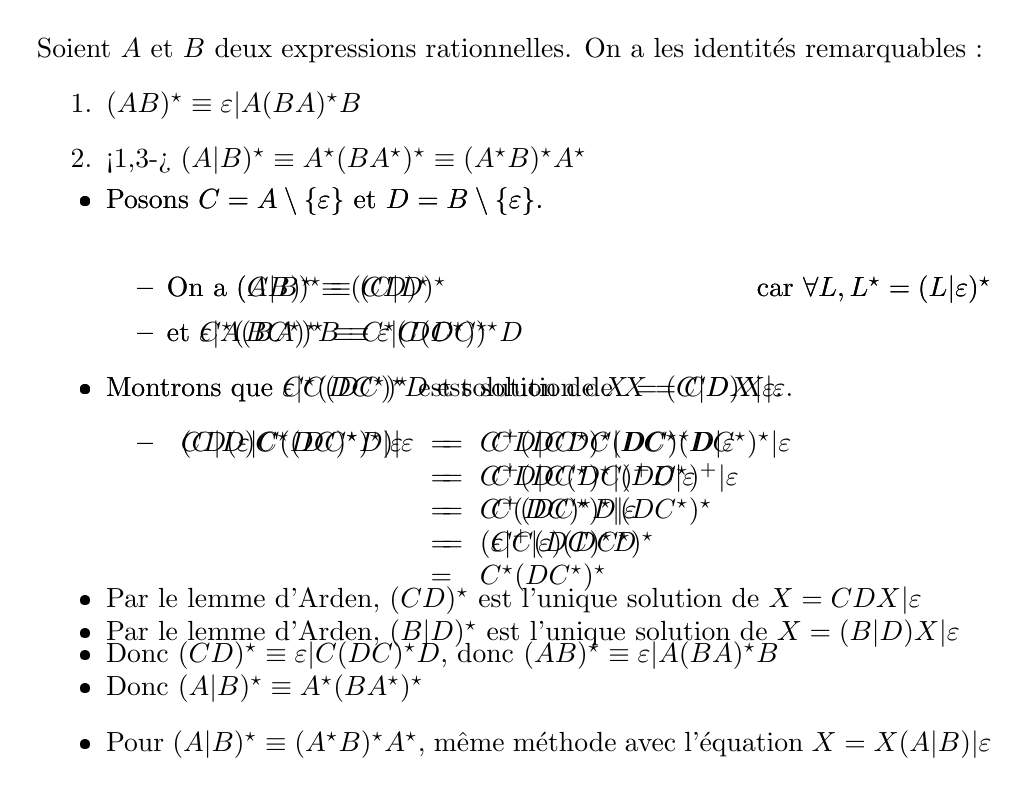
\begin{tikzpicture}

    \draw (10,10) node[below]{\begin{minipage}{\textwidth}
        Soient $A$ et $B$ deux expressions rationnelles. On a les identités remarquables : 
        \begin{enumerate}
        \item       \structure{$(AB)^\star \equiv \varepsilon | A(BA)^\star B$}
        \item<1,3-> \structure{$(A | B)^\star \equiv A^\star (B A^\star)^\star  \equiv (A^\star B)^\star A^\star$}
        \end{enumerate}
    \end{minipage}};

    \draw<2|handout:1> (10,8.1) node[below]{\begin{minipage}{\textwidth}
        \begin{itemize}
        \item Posons $C = A \setminus \{\varepsilon\}$ et $D = B \setminus \{\varepsilon\}$.\\
          \begin{itemize}
          \item On a $(A B)^\star \equiv (C D)^\star$  \hspace\fill car $\forall L, L^\star = (L | \varepsilon)^\star$
          \item et $\varepsilon  | A (B A)^\star B \equiv \varepsilon | C (D C)^\star D$
          \end{itemize}
        \item Montrons que $\varepsilon | C (D C)^\star D$ est solution de $X = CD X | \varepsilon$.
          \begin{itemize}
          \item $\begin{array}[t]{rclrcl}
            \structure{CD (\example{\varepsilon | C (D C)^\star D}) | \varepsilon}
            & = & CD | CD C (D C)^\star D | \varepsilon\\
            & = & CD | C (D C)^+ D | \varepsilon\\
            & = & C (D C)^\star D | \varepsilon\\
            & = & \example{\varepsilon | C (D C)^\star D}\\
          \end{array}
            $
          \end{itemize}
        \item Par le lemme d'Arden, $(CD)^\star$ est \alert{l'unique} solution de $X = CD X | \varepsilon$
        \item Donc $(CD)^\star \equiv \varepsilon | C (D C)^\star D$, donc $(AB)^\star \equiv \varepsilon | A (BA)^\star B$
        \end{itemize}
    \end{minipage}};

    \uncover<3-|handout:2>{
      \draw (10,8.1) node[below]{\begin{minipage}{\textwidth}
          \begin{itemize}
          \item Posons $C = A \setminus \{\varepsilon\}$ et $D = B \setminus \{\varepsilon\}$.\\
            \begin{itemize}
            \item On a $(C | B)^\star \equiv (C | D)^\star$ \hspace\fill car $\forall L, L^\star = (L | \varepsilon)^\star$
            \item et $C^\star (B C^\star)^\star \equiv C^\star (D C^\star)^\star$
            \end{itemize}
          \item Montrons que $C^\star (DC^\star)^\star$ est solution de $X = (C|D) X | \varepsilon$.
            \begin{itemize}
            \item $\begin{array}[t]{rclrcl}
              \structure{(C|D) \example{C^\star (DC^\star)^\star} | \varepsilon}
              & = & C^+ (DC^\star)^\star | D C^\star (DC^\star)^\star | \varepsilon\\
              & = & C^+ (DC^\star)^\star | (DC^\star)^+ | \varepsilon\\
              & = & C^+ (DC^\star)^\star | (DC^\star)^\star\\
              & = & (C^+|\varepsilon) (DC^\star)^\star\\
              & = & \example{C^\star (DC^\star)^\star}\\
            \end{array}
              $
            \end{itemize}
          \item Par le lemme d'Arden, $(B |D)^\star$ est \alert{l'unique} solution de $X = (B|D) X | \varepsilon$
          \item Donc $(A | B)^\star \equiv A^\star (B A^\star)^\star$
          \item Pour $(A | B)^\star \equiv (A^\star B)^\star A^\star$, même méthode avec l'équation $X = X (A|B) | \varepsilon$
          \end{itemize}
      \end{minipage}};
    }    
  \end{tikzpicture}
\end{frame}


\endgroup

% 
%\section{Des expressions rationnelles aux automates}
% 
%\subsection{Génération d'un automate fini non-déterministe}
%% SPDX-License-Identifier: CC-BY-SA-4.0
% Author: Matthieu Perrin
% Part: 
% Section: 
% Sub-section: 
% Frame: 

\begingroup

\begin{frame}{Génération d'analyseur lexical}

  \onBlock[top]{Problème}{
    \begin{description}
    \item[Entrée :] une expression rationnelle $r$
    \item[Sortie :] un \alert{analyseur lexical} pour le langage $\mathcal{L}(r)$
      \begin{itemize}
      \item Programme qui décide si son entrée appartient à $\mathcal{L}(r)$
      \end{itemize}
    \end{description}
  }

  \on[y=-3mm]{
    \begin{tikzpicture}
      \node[smBox, minimum width=3cm, minimum height=1.2cm] (exp) at (0,0) {Expression\\rationnelle};
      \node[smBox, minimum width=3cm, minimum height=1.2cm] (lex) at (6,0) {Analyseur\\lexical};
      
      \node[example, above] at (exp.north) {$a (b|c)^\star$};
      \node[example, above] at (lex.north) {$abc \rightarrow \cmark$, $bac \rightarrow \xmark$ };
      
      \path[-latex, structure, dashed] (exp) edge node[above]{JFlex} node[below]{Grep} (lex);
    \end{tikzpicture}
  }

\end{frame}

\endgroup

%% SPDX-License-Identifier: CC-BY-SA-4.0
% Author: Matthieu Perrin
% Part: 
% Section: 
% Sub-section: 
% Frame: 

\begingroup

\begin{frame}{Génération d'un automate}
  \SetKwData{Input}{motif}

  \vspace{-2cm}
  Soit $\Sigma$ un alphabet.

  \begin{minipage}{8cm}
    \begin{block}{Théorème}
      Tout langage rationnel
      est reconnaissable par un automate fini non-déterministe
      $$ \alert{\textsc{rat}_\Sigma \subseteq  \textsc{rec}_\Sigma} $$
    \end{block}
  \end{minipage}
  \begin{block}{Démonstration}
    Algorithme de Thompson
    \begin{description}
    \item [Entrée :] expression rationnelle \structure{$\Input \in \textsc{rat}_\Sigma$}
    \item [Sortie :] automate fini non-déterministe \structure{$A$} tel que $\mathcal{L}(A) = \mathcal{S}(\Input)$ 
      \begin{itemize}
      \item par récurrence sur la structure de $\Input$
      \item construit des automates \alert{normalisés}
      \end{itemize}
    \end{description}
  \end{block}

  \vspace{-6.7cm}\hspace\fill
  \begin{minipage}{2.5cm}
    \centering
    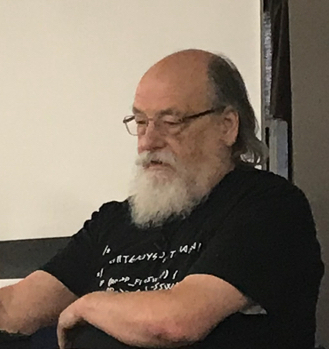
\includegraphics[width=2.5cm]{img/Thompson}
    
    Ken Thompson\footnote[frame,1]{Prix Turing 1983 avec Dennis Ritchie pour le développement d'Unix}
  \end{minipage}\hspace{5mm}
\end{frame}
\endgroup

%% SPDX-License-Identifier: CC-BY-SA-4.0
% Author: Matthieu Perrin
% Part: 
% Section: 
% Sub-section: 
% Frame: 

\begingroup

\begin{frame}{Automate normalisé}

  Soit $A = \langle \Sigma, Q, I, F, \mu\rangle$ un automate fini. 

  \begin{block}{Définition -- Automate unitaire}
    $A$ est dit \structure{unitaire} s'il ne possède qu'un seul état initial :
    $\alert{\exists q_0 \in Q, I = \{q_0\}}.$
  \end{block}

  \begin{block}{Définition -- Automate standard}
    $A$ est dit \structure{standard} si :
    \begin{enumerate}
    \item il est \alert{unitaire}
    \item aucune transition n'arrive sur l'état initial :
    $\alert{\forall q\in Q, \forall a\in \Sigma, q \xrightarrow{a} q_0 \notin \mu}.$
    \end{enumerate}
  \end{block}

  \begin{block}{Définition -- Automate normalisé}
    $A$ est dit \structure{normalisé} si :
    \begin{enumerate}
    \item il est \alert{standard}
    \item il ne possède qu'un seul état final : $\alert{\exists f \in Q, F = \{f\}}.$
    \item aucune transition n'a pour origine l'état final :
    $\alert{\forall q\in Q, \forall a\in \Sigma, \langle f, a, q\rangle \notin \mu}.$
    \end{enumerate}
  \end{block}
\end{frame}
\endgroup

%% SPDX-License-Identifier: CC-BY-SA-4.0
% Author: Matthieu Perrin
% Part: 
% Section: 
% Sub-section: 
% Frame: 

\begingroup

\begin{frame}{Normalisation d'un automate fini}

  \onBlock[top=-3mm]{Théorème -- Normalisation}{
      Soit $\Sigma$ un alphabet et $L \in \textsc{rec}_\Sigma$.
      $L$ est reconnu par un automate normalisé.
  }

  \onBlock[y=5mm]{Démonstration}{
    Soit $\langle \Sigma, Q, I, F, \rightarrow \rangle$ un automate qui reconnaît $L$.
    \begin{itemize}
    \item Soient $i, f \notin Q$
    \item Soit $\rightarrow' \,=\, \rightarrow \,\cup\,
      \structure{\{\langle i, \varepsilon, q\rangle \mid q \in I\}} \,\cup\,
      \alert{\{\langle q, \varepsilon, f\rangle \mid q \in F\}}$
    \end{itemize}
    Alors $L$ est reconnu par l'automate normalisé :
    $$\langle \Sigma, Q \cup \{i, f\}, \structure{\{i\}}, \alert{\{f\}}, \rightarrow' \rangle$$
  }

  \onExampleBlock[y=-15mm]{Exemple}{}
  
  \on[bottom,x=-.25\textwidth]{
    \begin{tikzpicture}[automaton]
      \state            (2)                     {$2$};
      \state[initial]   (0) [above left =of 2]  {$0$};
      \state[initial]   (1) [below left =of 2]  {$1$};
      \state[accepting] (3) [above right=of 2]  {$3$};
      \state[accepting] (4) [below right=of 2]  {$4$};
      
      \path  (0) edge node {$a$} (3);
      \path  (0) edge node {$b$} (2);
      \path  (1) edge node {$a$} (2);
      \path  (1) edge node {$b$} (4);
      \path  (2) edge node {$a$} (3);
      \path  (2) edge node {$b$} (4);
    \end{tikzpicture}
  }
  
  \on[bottom,x=.25\textwidth]{
    \begin{tikzpicture}[automaton]
      \state                     (2)                     {$2$};
      \state                     (0) [above left =of 2]  {$0$};
      \state                     (1) [below left =of 2]  {$1$};
      \state                     (3) [above right=of 2]  {$3$};
      \state                     (4) [below right=of 2]  {$4$};
      \state[initial, structure] (i) [above left =of 1]  {$i$};
      \state[accepting, alert]   (f) [above right=of 4]  {$f$};

      \path            (0) edge node {$a$} (3);
      \path            (0) edge node {$b$} (2);
      \path            (1) edge node {$a$} (2);
      \path            (1) edge node {$b$} (4);
      \path            (2) edge node {$a$} (3);
      \path            (2) edge node {$b$} (4);
      \path[structure] (i) edge node {$\varepsilon$} (0);
      \path[structure] (i) edge node {$\varepsilon$} (1);
      \path[alert]     (3) edge node {$\varepsilon$} (f);
      \path[alert]     (4) edge node {$\varepsilon$} (f);
    \end{tikzpicture}
  }
  
\end{frame}


\endgroup

%% SPDX-License-Identifier: CC-BY-SA-4.0
% Author: Matthieu Perrin
% Part: 
% Section: 
% Sub-section: 
% Frame: 

\begingroup

\begin{frame}[fragile]{Algorithme de Thompson}
  \begingroup
  \renewcommand{\emph}[1]{\structure{#1}} 
  \vspace{-1mm}
  
  ~\hspace{-5mm}
  \begin{tikzpicture}
    
    \draw[white] (0,-.5) rectangle (11.3,7.5);
    \draw (5,4.85) node{\begin{minipage}{15cm}\scalebox{.7}{\begin{algorithm}[H]
            \SetKwProg{Fn}{Fonction}{}{fin}
            \SetKw{Let}{soit}
            \SetKw{Lets}{soient}
            \SetKw{Retourner}{retourner}
            \SetKwFunction{Thompson}{thompson}
            \SetKwData{Input}{motif}
            \SetKwIF{Si}{SinonSi}{Sinon}{si}{}{sinon si}{sinon}{fin si}
            
            \Fn{\Thompson(\Input : \textsc{regex}, $\Sigma$ : alphabet) : automate}{
              \Lets \alert{$q_0$}, \alert{$q_f$} deux nouveaux états\;
                \uSi{$\Input = \emptyset$}{\uncover<2->{
                    $Q \,\leftarrow \{\alert{q_0}, \alert{q_f}\}$\;
                    $\mu \,\,\leftarrow \emptyset$\;
                }}\uSinonSi{$\Input = a\in \Sigma \cup \{\varepsilon\}$}{\uncover<3->{
                    $Q \,\leftarrow \{\alert{q_0}, \alert{q_f}\}$\;
                    $\mu \,\,\leftarrow \{ \alert{\langle q_0, a, q_f \rangle} \}$\;
                }}\uSinonSi{$\Input = u | v$}{\uncover<4->{
                    $\langle \structure{\Sigma}, \structure{Q_u}, \{\structure{u_0}\}, \{\structure{u_f}\}, \structure{\lambda} \rangle \leftarrow \structure{\Thompson(u, \Sigma)}$\;
                    $\langle \example{\Sigma}, \example{Q_v}, \{\example{v_0}\}, \{\example{v_f}\}, \example{\tau}\, \rangle \leftarrow \example{\Thompson(v, \Sigma)}$\;

                    $Q \,\leftarrow \structure{Q_u} \cup \example{Q_v} \cup \{\alert{q_0}, \alert{q_f}\}$\;
                    $\mu \,\,\leftarrow \structure{\lambda} \cup \example{\tau} \cup \left\{\begin{array}{l}
                    \alert{\langle q_0, \varepsilon, u_0 \rangle}, \alert{\langle q_0, \varepsilon, v_0 \rangle}, \\
                    \alert{\langle u_f, \varepsilon, q_f \rangle}, \alert{\langle v_f, \varepsilon, q_f \rangle}
                    \end{array}\right\} $\;
                }}\uSinonSi{$\Input = u \cdot v$}{\uncover<5->{
                    $\langle \structure{\Sigma}, \structure{Q_u}, \{\structure{u_0}\}, \{\structure{u_f}\}, \structure{\lambda} \rangle \leftarrow \structure{\Thompson(u, \Sigma)}$\;
                    $\langle \example{\Sigma}, \example{Q_v}, \{\example{v_0}\}, \{\example{v_f}\}, \example{\tau}\, \rangle \leftarrow \example{\Thompson(v, \Sigma)}$\;

                    $Q \,\leftarrow \structure{Q_u} \cup \example{Q_v}$\;
                    $q_0 \leftarrow \structure{u_0}$;~
                    $q_f \leftarrow \example{v_f}$\;
                    $\mu \,\,\leftarrow \structure{\lambda} \cup \example{\tau} \cup \{\alert{\langle u_f, \varepsilon, v_0 \rangle}\} $\;
                }}\SinonSi{$\Input = u^\star$}{\uncover<6->{
                    $\langle \structure{\Sigma}, \structure{Q_u}, \{\structure{u_0}\}, \{\structure{u_f}\}, \structure{\lambda} \rangle \leftarrow \structure{\Thompson(u, \Sigma)}$\;

                    $Q \,\leftarrow \structure{Q_u} \cup \{\alert{q_0}, \alert{q_f}\}$\;
                    $\mu \,\,\leftarrow \structure{\lambda} \cup \{\alert{\langle q_0, \varepsilon, u_0 \rangle}, \alert{\langle u_f, \varepsilon, u_0 \rangle}, \alert{\langle u_f, \varepsilon, q_f \rangle}\}$\;
                }}
              
              \Retourner $\langle \Sigma, Q, \{q_0\}, \{q_f\}, \mu \rangle$\;
            }
    \end{algorithm}}\end{minipage}};


    \draw<2-> (3.2,7.5) node[right]{\scalebox{.65}{\begin{tikzpicture}[shorten >=1pt,node distance=1.5cm,on grid,auto]
      \node [state,initial, initial text=, alert, fill=alert!20] (a1)   {$q_0$}; 
      \node [state,accepting, alert, fill=alert!20] (a2) [right=of a1]  {$q_f$}; 
    \end{tikzpicture}}};

    \draw<3-> (6.2,7.5) node[right]{\scalebox{.65}{\begin{tikzpicture}[shorten >=1pt,node distance=1.5cm,on grid,auto]
      \node [state,initial, initial text=, alert, fill=alert!20] (b1)   {$q_0$}; 
      \node [state,accepting, alert, fill=alert!20] (b2) [right=of a1]  {$q_f$}; 
      \path [alert,->]    (b1) edge node{$a$} (b2);
    \end{tikzpicture}}};


    \draw<4-> (3.2,5.75) node[right]{\scalebox{.65}{\begin{tikzpicture}[shorten >=1pt,node distance=1.5cm,on grid,auto]
      \node [state,initial, initial text=, alert, fill=alert!20] (c1)   {$q_0$};

      \node [state, structure, fill=structure!20] (c2) [above right=of c1]  {$u_0$};
      \node (c3) [right=of c2, cloud, cloud puffs=11 ,cloud puff arc=120, aspect=2, inner ysep=1em, fill=structure!20] {};
      \node [state, structure, fill=structure!20] (c4) [right=of c3]  {$u_f$};
      
      \node [state, example, fill=example!20] (c5) [below right= of c1]  {$v_0$};
      \node (c6) [right=of c5, cloud, cloud puffs=10,cloud puff arc=100, aspect=2, inner ysep=1em, fill=example!20] {};
      \node [state, example, fill=example!20] (c7) [right= of c6]  {$v_f$};

      \node [state,accepting, alert, fill=alert!20] (c8) [above right= of c7]  {$q_f$};

      \path [->, alert]    (c1) edge node[below] {$\varepsilon$} (c2);
      \path [->, alert]    (c1) edge node[above] {$\varepsilon$} (c5);
      \path [->, alert]    (c4) edge node[below] {$\varepsilon$} (c8);
      \path [->, alert]    (c7) edge node[above] {$\varepsilon$} (c8);

      \path [dashed,->, structure]    (c2) edge[bend left=5mm]  (c4);
      \path [dashed,->, structure]    (c2) edge  (c4);
      \path [dashed,->, structure]    (c2) edge[bend right=5mm] (c4);
      \path [dashed,->, example]    (c5) edge[bend left=5mm]  (c7);
      \path [dashed,->, example]    (c5) edge  (c7);
      \path [dashed,->, example]    (c5) edge[bend right=5mm] (c7);
    \end{tikzpicture}}};

    \draw<5-> (3.2,3.75) node[right]{\scalebox{.65}{\begin{tikzpicture}[shorten >=1pt,node distance=1.5cm,on grid,auto]
      \node [state,initial, initial text=, structure, fill=structure!20] (d2)  {$u_0$};
      \node (d3) [right=of d2, cloud, cloud puffs=11 ,cloud puff arc=120, aspect=2, inner ysep=1em, fill=structure!20] {};
      \node [state, structure, fill=structure!20] (d4) [right=of d3]  {$u_f$};
      
      \node [state, example, fill=example!20] (d5) [right= of d4]  {$v_0$};
      \node (d6) [right=of d5, cloud, cloud puffs=10,cloud puff arc=100, aspect=2, inner ysep=1em, fill=example!20] {};
      \node [state,accepting, example, fill=example!20] (d7) [right= of d6]  {$v_f$};

      \path [->, alert]  (d4) edge node[above] {$\varepsilon$} (d5);

      \path [dashed,->, structure]    (d2) edge[bend left=5mm]  (d4);
      \path [dashed,->, structure]    (d2) edge  (d4);
      \path [dashed,->, structure]    (d2) edge[bend right=5mm] (d4);
      \path [dashed,->, example]    (d5) edge[bend left=5mm]  (d7);
      \path [dashed,->, example]    (d5) edge  (d7);
      \path [dashed,->, example]    (d5) edge[bend right=5mm] (d7);
    \end{tikzpicture}}};
    
    \draw<6-> (3.2,2) node[right]{\scalebox{.65}{\begin{tikzpicture}[shorten >=1pt,node distance=1.5cm,on grid,auto]
      \node [state,initial, initial text=, alert, fill=alert!20] (e1)   {$q_0$};
      \node [state, structure, fill=structure!20] (e2) [right=of e1] {$u_0$};
      \node (e3) [right=of e2, cloud, cloud puffs=11 ,cloud puff arc=120, aspect=2, inner ysep=1em, fill=structure!20] {};
      \node [state, structure, fill=structure!20] (e4) [right=of e3]  {$u_f$};
      \node [state,accepting, alert, fill=alert!20] (e5) [below= of e2]  {$q_f$};
      
      \path [->, alert]  (e1) edge node[above] {$\varepsilon$} (e2);
      \path [->, alert]  (e2) edge node[left] {$\varepsilon$} (e5);
      \path [->, alert]  (e4) edge[bend left=2cm] node[below] {$\varepsilon$} (e2);

      \path [dashed,->, structure]    (e2) edge[bend left=5mm]  (e4);
      \path [dashed,->, structure]    (e2) edge  (e4);
      \path [dashed,->, structure]    (e2) edge[bend right=5mm] (e4);
    \end{tikzpicture}}};

  \end{tikzpicture}
  \endgroup
\end{frame}


\endgroup

%% SPDX-License-Identifier: CC-BY-SA-4.0
% Author: Matthieu Perrin
% Part: 
% Section: 
% Sub-section: 
% Frame: 

\begingroup

\begin{frame}{Exemple d'utilisation du lemme de pompage}
  
  \tfBlock[top=-5mm]{Montrer que $L \eqdef \{a^nb^nc^n \mid n\in \mathbb{N}\}$ n'est pas algébrique}{
    Soit $\Sigma \eqdef \{a, b, c\}$.%
    \only<2-|handout>{
      Si $L$ est algébrique, $L$ vérifie le lemme de pompage :

      \vspace{-4mm}
      $$
      \begin{array}{c}
        \structure{\exists N\in \mathbb{N}}, \alert{\forall u\in L, |u| \ge N} \Rightarrow (\structure{\exists v, w, x, y, z\in \Sigma^\star}, \\
        u = v \cdot w \cdot x\cdot y \cdot z \land w \cdot y\neq \varepsilon \land |w\cdot x\cdot y| \le N \land \alert{\forall i \in \mathbb{N}}, v\cdot w^i\cdot x\cdot y^i \cdot z \in L)
      \end{array}
      $$
      \vspace{-2mm}
      
      \structure{Soit $N$ donné par le lemme pompage}.
    }
    
    \only<3-|handout>{%
      \alert{Posons $u = a^N b^N c^N$. On a bien $u\in L$ et $|u| = 3N \ge N$}.\\
      \structure{Soit $v \cdot w \cdot x\cdot y \cdot z$ la décomposition de $u$ donnée par le lemme de pompage}. 
    }
  }
  
  \tf<4-|handout>[y=-10mm]{
    \begin{smArray}[width=4mm, height=3mm, name={$u=$}]
      \smCell[\smNone]{\alert{$a$}}      \smCoord{(a1)}
      \smCell[\smNone]{\alert{$\cdots$}}               
      \smCell[\smNone]{\alert{$a$}}      \smCoord{(an)}
      \smCell[\smNone]{\alert{$\cdot$}}               
      \smCell[\smNone]{\alert{$b$}}      \smCoord{(b1)}
      \smCell[\smNone]{\alert{$\cdots$}}               
      \smCell[\smNone]{\alert{$b$}}      \smCoord{(bn)}
      \smCell[\smNone]{\alert{$\cdot$}}               
      \smCell[\smNone]{\alert{$c$}}      \smCoord{(c1)}
      \smCell[\smNone]{\alert{$\cdots$}}               
      \smCell[\smNone]{\alert{$c$}}      \smCoord{(cn)}
      
      \draw [decorate, decoration={brace, amplitude=5pt}] ([xshift=1mm]a1.north west) -- ([xshift=-1mm]an.north east) node[midway,yshift=4mm]{$N$};
      \draw [decorate, decoration={brace, amplitude=5pt}] ([xshift=1mm]b1.north west) -- ([xshift=-1mm]bn.north east) node[midway,yshift=4mm]{$N$};
      \draw [decorate, decoration={brace, amplitude=5pt}] ([xshift=1mm]c1.north west) -- ([xshift=-1mm]cn.north east) node[midway,yshift=4mm]{$N$};

      \draw [decorate, decoration={brace, amplitude=5pt, mirror}] ([xshift=1mm]an.south west) -- ([xshift=-1mm]b1.south east) node[midway,yshift=-4mm]{$|wxy|\le N$};
      \draw [decorate, decoration={brace, amplitude=5pt, mirror}] ([xshift=1mm]bn.south west) -- ([xshift=-1mm]c1.south east) node[midway,yshift=-4mm]{$|wxy|\le N$};
    \end{smArray}       
  }

  \tf<5-|handout>[text, bottom=-1mm]{
    \begin{itemize}
    \item Comme $wy \neq \varepsilon$, $\alpha = wy[1] \in \Sigma$ est une lettre de $wy$.
    \item Comme $|wxy| \le N$, il existe $\beta \in \Sigma$ tel que $\beta$ n'est pas une lettre de $wy$. 
    \item \alert{Posons $i=2$}. $|v \cdot w^2 \cdot x\cdot  y^2\cdot   z|_\alpha > |v\cdot  w^2\cdot  x\cdot  y^2\cdot   z|_\beta$, donc $v\cdot  w^2\cdot  x\cdot  y^2\cdot   z\notin L$. 
    \end{itemize}
    Absurde ! Donc $L$ n'est pas algébrique. 
  }

  \tfExampleBlock<-4>[y=-25mm]{On sait}{}

  \tf<1>[y=-25mm, anchor=north, text]{
    \begin{itemize}
    \item $\begin{array}[t]{l}
      \alert{\forall L \in \textsc{alg}_\Sigma}, \structure{\exists N\in \mathbb{N}}, \forall u\in L, |u| \ge N \Rightarrow (\exists v, w, x, y, z\in \Sigma^\star, \\
      u = v w x y z \land w y\neq \varepsilon \land |wxy| \le N \land \forall i \in \mathbb{N}, v w^i x y^i z \in L)
    \end{array}$
    \end{itemize}
  }

  \tf<2-4>[y=-25mm, anchor=north, left=.35\textwidth]{
    \begin{itemize}
    \item $L \in \textsc{alg}_\Sigma$
    \item<3-> $v, w, x, y, z\in \Sigma^\star$
    \end{itemize}
  }
  
  \tf<2-4>[y=-25mm, anchor=north, width=.35\textwidth]{
    \begin{itemize}
    \item $N \in \mathbb{N}$
    \item<3-> $wy\neq \varepsilon$
    \end{itemize}
  }
  
  \tf<3-4>[y=-25mm, anchor=north, right=.35\textwidth]{
    \begin{itemize}
    \item $v \cdot w \cdot x \cdot y \cdot z = a^N b^N c^N$
    \item $\alert{|wxy| \le N}$
    \end{itemize}
  }
  
\end{frame}

\endgroup

% 
%\subsection{Déterminisation d'un automate fini}
%% SPDX-License-Identifier: CC-BY-SA-4.0
% Author: Matthieu Perrin
% Part: 
% Section: 
% Sub-section: 
% Frame: 

\begingroup

\begin{frame}{Génération d'analyseur lexical}

  \onBlock[top]{Problème}{
    \begin{description}
    \item[Entrée :] une expression rationnelle $r$
    \item[Sortie :] un \alert{analyseur lexical} pour le langage $\mathcal{L}(r)$
      \begin{itemize}
      \item Programme qui décide si son entrée appartient à $\mathcal{L}(r)$
      \end{itemize}
    \end{description}
  }

  \on[y=-3mm]{
    \begin{tikzpicture}
      \node[smBox, minimum width=3cm, minimum height=1.2cm] (exp) at (0,0) {Expression\\rationnelle};
      \node[smBox, minimum width=3cm, minimum height=1.2cm] (lex) at (6,0) {Analyseur\\lexical};
      
      \node[example, above] at (exp.north) {$a (b|c)^\star$};
      \node[example, above] at (lex.north) {$abc \rightarrow \cmark$, $bac \rightarrow \xmark$ };
      
      \path[-latex, structure, dashed] (exp) edge node[above]{JFlex} node[below]{Grep} (lex);
    \end{tikzpicture}
  }

\end{frame}

\endgroup

%% SPDX-License-Identifier: CC-BY-SA-4.0
% Author: Matthieu Perrin
% Part: 
% Section: 
% Sub-section: 
% Frame: 

\begingroup

\begin{frame}{Automates déterministes}

  Soit $A = \langle \Sigma, Q, I, F, \mu \rangle$ un AFN.
  
  \begin{block}{Définition -- Automate fini déterministe (AFD)}
    On dit que $A$ est \structure{déterministe} si toutes les conditions sont vérifiées
    \begin{description}[fonction partielle :]
    \item[$\varepsilon$-libre :] $A$ ne possède pas d'$\varepsilon$-transition

      $$\alert{\mu \subseteq Q \times \Sigma \times Q}$$

    \item[unitaire :] $A$ ne possède pas qu'un seul état initial

      $$\alert{\exists q_0\in Q, I = \{q_0\}}$$

    \item[fonction partielle :] pour chaque état $q$ et chaque symbole $a$, il existe au plus une transition sortant de $q$ étiquetée $a$

      $$\alert{\forall q, q_1, q_2\in Q,  \forall a\in \Sigma, \left(\structure{q\xrightarrow{a} q_1} \in \mu \land \structure{q\xrightarrow{a} q_2} \in \mu\right) \structure{\Rightarrow q_1 = q_2}}$$
    \end{description}
  \end{block}

\end{frame}

\endgroup

%% SPDX-License-Identifier: CC-BY-SA-4.0
% Author: Matthieu Perrin
% Part: 
% Section: 
% Sub-section: 
% Frame: 

\begingroup

\begin{frame}{Relation d'équivalence}

  Soit $\bowtie$ une relation binaire homogène sur un ensemble $E$.
  \begin{block}{Définition -- Relation d'équivalence}
    $\bowtie$ est une \structure{relation d'équivalence} si elle est \alert{réflexive}, \alert{transitive} et \alert{symétrique}.
  \end{block}

  \begin{block}{Définition -- Classe d'équivalence}
    La \structure{classe d'équivalence} d'un élément $x \in E$, notée $\alert{[x]_{\bowtie}}$ est l'ensemble des éléments de $E$ en relation avec $x$ :
    $$\alert{[x]_{\bowtie} \eqdef \{y\in E | y \bowtie x\}}$$
  \end{block}

  \begin{block}{Définition -- Ensemble quotient}
    L'\structure{ensemble quotient} de $E$ par $\bowtie$, noté $\alert{E/_{\bowtie}}$, est l'ensemble des classes d'équivalence des éléments de $E$.

    $$\alert{ E/_{\bowtie} \eqdef \bigcup_{x\in E}\left\{[x]_{\bowtie}\right\}}$$
  \end{block}
\end{frame}

\endgroup

%% SPDX-License-Identifier: CC-BY-SA-4.0
% Author: Matthieu Perrin
% Part: 
% Section: 
% Sub-section: 
% Frame: 

\begingroup

\begin{frame}{Interprétation ubiquitaire du non-déterminisme}

  \onBlock[top=-3mm]{Interprétation du non-déterminisme comme de l'ubiquité}{
    \begin{itemize}
    \item L'automate se trouve dans un sous-ensemble des états
    \item Le mot est reconnu si l'un des états du sous-ensemble est final
    \item Ces sous-ensembles forment un nouvel automate, qui est déterministe
    \end{itemize}
  }

  \onExampleBlock[y=1mm]{Exemple : reconnaissance de $\alert{abc}$ par l'automate suivant}{
    \vspace{-2mm}
    $$
    \alertb<1>{\{1\}}
    \uncover<2->{\xrightarrow{a} \alert<2> {\{2, 3, 5, 7, 9, 10\}}}
    \uncover<3->{\xrightarrow{b} \alertb<3>{\{3, 4, 5, 7, 8, 10\}}}
    \uncover<4->{\xrightarrow{c} \alertb<4>{\{3, 5, 6, 7, 8, 10\}}}
    $$
  }
  
  \on[bottom] {
    \begin{tikzpicture}[automaton]
      \state[initial,   alert ob=<1> ] (1)  at (0,2) {$1$};    
      \state[           alert on=<2> ] (2)  at (1,2) {$2$};    
      \state[           alert on=<2->] (3)  at (4,2) {$3$};    
      \state[           alert ob=<3> ] (4)  at (5,2) {$4$};    
      \state[           alert on=<2->] (5)  at (4,0) {$5$};    
      \state[           alert ob=<4->] (6)  at (5,0) {$6$};    
      \state[           alert on=<2->] (7)  at (3,1) {$7$};    
      \state[           alert ob=<3->] (8)  at (6,1) {$8$};    
      \state[           alert on=<2> ] (9)  at (2,2) {$9$};    
      \state[accepting, alert on=<2->] (10) at (2,0) {$10$};   

      \path (1) edge node {$a$}           (2);
      \path (3) edge node {$b$}           (4);
      \path (5) edge node {$c$}           (6);
      \path (7) edge node {$\varepsilon$} (3);
      \path (7) edge node {$\varepsilon$} (5);
      \path (4) edge node {$\varepsilon$} (8);
      \path (6) edge node {$\varepsilon$} (8);
      \path (9) edge node {$\varepsilon$} (7);
      \path (8) edge node {$\varepsilon$} (7);
      \path (7) edge node {$\varepsilon$} (10);
      \path (2) edge node {$\varepsilon$} (9);
    \end{tikzpicture}
  }

\end{frame}

\endgroup

%% SPDX-License-Identifier: CC-BY-SA-4.0
% Author: Matthieu Perrin
% Part: 
% Section: 
% Sub-section: 
% Frame: 

\begingroup

\SetKwFunction{RabinScott}{rabin\_scott}
\SetKwFunction{Fermeture}{$\varepsilon$-fermeture}

\begin{frame}[fragile]{Méthode des sous-ensembles de Rabin et Scott}

  \tf[top]{\footnotesize
    \begin{algorithm}[H]
      \Fn{\RabinScott($A = \langle \Sigma, Q, I, F, \mu \rangle$ : automate) : automate}{
        \tfExample<2-4>{$i' \leftarrow \Fermeture (A, I)$}\;
        $Q' \leftarrow \{i'\}$\;
        $\mu' \leftarrow \emptyset$\;
        \Tantque{\tfAlert<5,6>{$\exists S\in Q', \exists a\in \Sigma, \forall S'\in Q', \langle S, a, S' \rangle \notin \mu'$}}{
          \tfStructure<6>{$S' \leftarrow \Fermeture (A, \{q'\in Q | \exists q\in S, \langle q, a, q' \rangle \in \mu \})$}\;
          $Q' \leftarrow Q \cup \{S\}$\;
          $\mu' \leftarrow \mu' \cup \{\langle S, a, S' \rangle\}$\;
        }
        \tfAlert<7>{$F' \leftarrow \{S \in Q' | S\cap F \neq \emptyset\}$}\;
        \Retourner $\langle \Sigma, Q', \{i'\}, F', \mu' \rangle$\;
      }
      \Fn{\Fermeture($A = \langle \Sigma, Q, I, F, \mu \rangle$ : automate, $S$ : ensemble) : ensemble}{
        \uSi{\tfStructure<2-4>{$\exists \langle q, \varepsilon, q' \rangle \in \mu : q\in S \land q' \notin S$}}{
          \Retourner $\Fermeture(A, S \cup \{q'\})$\;
        }\lSinon{\Retourner $S$}
      }
    \end{algorithm}
  }

  \tfExampleBlock[right=3cm, top]{Exemple}{\footnotesize
    \begin{tikzpicture}[smAutomaton, node distance=1cm]
      \smState[\smInitial                 \smExample<2-6>] (0) at (0.0,1.2) {$0$};
      \smState[\smAccepting                              ] (1) at (1.2,1.2) {$1$};
      \smState[                                          ] (2) at (2.4,1.2) {$2$};
      \smState[\smInitial                 \smExample<2-6>] (3) at (0.0,0.0) {$3$};
      \smState[            \smStructure<2>\smExample<3-6>] (4) at (1.2,0.0) {$4$};
      \smState[            \smStructure<3>\smExample<4-6>] (5) at (2.4,0.0) {$5$};

      \smPath[\smStructure<2>  ] (3) edge             node {$\varepsilon$} (4);
      \smPath[\smStructure<3,6>] (4) edge             node {$\varepsilon$} (5);
      \smPath[                 ] (2) edge             node {$b$}           (1);
      \smPath[\smAlert<5>      ] (5) edge[bend left ] node {$a$}           (2);
      \smPath[                 ] (2) edge[bend left ] node {$a$}           (5);
      \smPath[\smAlert<6>      ] (4) edge[bend left ] node {$b$}           (1);
      \smPath[                 ] (1) edge[bend left ] node {$b$}           (4);
      \smPath[                 ] (1) edge[loop above] node {$a$}           (1);
      \smPath[                 ] (2) edge[loop above] node {$b$}           (2);
      \smPath[\smAlert<6>      ] (4) edge[loop below] node {$b$}           (4);
      \smPath[\smAlert<5>      ] (5) edge[loop below] node {$a$}           (5);
    \end{tikzpicture}
  }

  \tfExampleBlock<2-4>[bottom]{Calcul de l' $\varepsilon$-fermeture de $I$}{
    \vspace{-3mm}
    $$\begin{array}{rcl}
      i' &=& \Fermeture(A, I)\\
      &=& \Fermeture(A, \{0, 3\})\\
      &\uncover<3->{=}& \uncover<3->{\Fermeture(A, \{0, 3, 4\})}\\
      &\uncover<4->{=}& \uncover<4->{\Fermeture(A, \{0, 3, 4, 5\})}\\
      &\uncover<4->{=}& \uncover<4->{\{0, 3, 4, 5\}}\\
    \end{array}$$
  }  

  \tf<5-|handout>[bottom=-5mm, x=-33mm] {\tiny
    \begin{tikzpicture}[smAutomaton]
      \draw[white] (-.5,-.5) -- (5.5,2.5);
      
      \smState<5-|handout> [\smInitial]   (a) at (0.4,1.0) {$A$}; 
      \smState<6-|handout> []             (b) at (1.2,1.8) {$B$}; 
      \smState<7-|handout> [\smAccepting] (c) at (1.2,0.2) {$C$}; 
      \smState<8-|handout> [\smAccepting] (d) at (3.8,1.8) {$D$}; 
      \smState<9-|handout> [\smAccepting] (e) at (3.8,0.2) {$E$}; 
      \smState<10-|handout>[\smAccepting] (f) at (3.0,1.0) {$F$};
      \smState<10-|handout>[\smAccepting] (g) at (4.6,1.0) {$G$}; 
      \smState<12-|handout>[]             (h) at (2.0,1.0) {$H$}; 

      \only<5,6>{
        \smState[\smAlert] (empty) at (2,1) {?};
        \smPath<5>[\smAlert] (a) edge node {$a$} (empty);
        \smPath<6>[\smAlert] (a) edge node {$b$} (empty);
      }

      \smPath<6-|handout>  (a) edge[bend left ] node[swap] {$a$} (b);
      \smPath<7-|handout>  (a) edge[bend right] node       {$b$} (c);
      \smPath<8-|handout>  (b) edge[loop above] node       {$a$} (b);
      \smPath<8-|handout>  (b) edge             node       {$b$} (d);
      \smPath<9-|handout>  (c) edge             node       {$a$} (e);
      \smPath<9-|handout>  (c) edge[loop below] node       {$b$} (c);
      \smPath<10-|handout> (d) edge[bend right] node       {$a$} (f);
      \smPath<10-|handout> (d) edge[bend left ] node[swap] {$b$} (g);
      \smPath<11-|handout> (e) edge[loop below] node       {$a$} (e);
      \smPath<11-|handout> (e) edge[bend right] node       {$b$} (g);
      \smPath<12-|handout> (f) edge[bend right] node       {$a$} (e);
      \smPath<12-|handout> (f) edge             node       {$b$} (h);
      \smPath<13-|handout> (g) edge[bend right] node[swap] {$a$} (e);
      \smPath<13-|handout> (g) edge[loop right] node       {$b$} (g);
      \smPath<14-|handout> (h) edge[bend right] node       {$a$} (b);
      \smPath<14-|handout> (h) edge[bend left ] node[swap] {$b$} (c);
    \end{tikzpicture}
  }
  
  \tf<5-|handout>[bottom, x=.27\textwidth]{\footnotesize
    \begin{tabular}{|l|l|l|}
      \hline
      &
      \multicolumn{2}{c|}{\structure{\textbf{Entrée}}}\\
      \hline
      \structure{\textbf{\'Etat}} &
      $\structure{a}$ &
      $\structure{b}$ \\
      \hline
      $A=\{0,3,4,5\}$ \hspace\fill\structure{i}  &
      \only<5>{\alert{?}}\only<6-|handout> {$B=\{5, 2\}$} &
      \only<6> {\alert{?}}\only<7-|handout> {$C=\{1,4,5\}$} \\
      \uncover<6-|handout> {$B=\{5, 2\}$} &
      \uncover<8-|handout> {$B=\{5, 2\}$} &
      \uncover<8-|handout> {$D=\{1, 2\}$} \\
      \uncover<7-|handout> {$C=\{1,4,5\}$ \hspace\fill\structure{f}} &
      \uncover<9-|handout> {$E=\{1,2,5\}$} &
      \uncover<9-|handout> {$C=\{1,4,5\}$} \\
      \uncover<8-|handout> {$D=\{1,2\}$ \hspace\fill\structure{f}} &
      \uncover<10-|handout>{$F=\{1,5\}$} &
      \uncover<10-|handout>{$G=\{1,2,4,5\}$} \\
      \uncover<9-|handout> {$E=\{1,2,5\}$ \hspace\fill\structure{f}} &
      \uncover<11-|handout>{$E=\{1,2,5\}$} &
      \uncover<11-|handout>{$G=\{1,2,4,5\}$} \\
      \uncover<10-|handout>{$F=\{1,5\}$ \hspace\fill\structure{f}} &
      \uncover<12-|handout>{$E=\{1,2,5\}$} &
      \uncover<12-|handout>{$H=\{4,5\}$} \\
      \uncover<10-|handout>{$G=\{1,2,4,5\}$ \hspace\fill\structure{f}} &
      \uncover<13-|handout>{$E=\{1,2,5\}$} &
      \uncover<13-|handout>{$G=\{1,2,4,5\}$} \\
      \uncover<12-|handout>{$H=\{4,5\}$} &
      \uncover<14-|handout>{$B=\{5,2\}$} &
      \uncover<14-|handout>{$C=\{1,4,5\}$} \\
      \hline
    \end{tabular}
  }
  
\end{frame}

\endgroup

% 
%\subsection{Minimisation d'un automate fini déterministe}
%% SPDX-License-Identifier: CC-BY-SA-4.0
% Author: Matthieu Perrin
% Part: 
% Section: 
% Sub-section: 
% Frame: 

\begingroup

\begin{frame}{Génération d'analyseur lexical}

  \onBlock[top]{Problème}{
    \begin{description}
    \item[Entrée :] une expression rationnelle $r$
    \item[Sortie :] un \alert{analyseur lexical} pour le langage $\mathcal{L}(r)$
      \begin{itemize}
      \item Programme qui décide si son entrée appartient à $\mathcal{L}(r)$
      \end{itemize}
    \end{description}
  }

  \on[y=-3mm]{
    \begin{tikzpicture}
      \node[smBox, minimum width=3cm, minimum height=1.2cm] (exp) at (0,0) {Expression\\rationnelle};
      \node[smBox, minimum width=3cm, minimum height=1.2cm] (lex) at (6,0) {Analyseur\\lexical};
      
      \node[example, above] at (exp.north) {$a (b|c)^\star$};
      \node[example, above] at (lex.north) {$abc \rightarrow \cmark$, $bac \rightarrow \xmark$ };
      
      \path[-latex, structure, dashed] (exp) edge node[above]{JFlex} node[below]{Grep} (lex);
    \end{tikzpicture}
  }

\end{frame}

\endgroup

%% SPDX-License-Identifier: CC-BY-SA-4.0
% Author: Matthieu Perrin
% Part: 
% Section: 
% Sub-section: 
% Frame: 

\begingroup

\begin{frame}{Minimalité d'un automate fini déterministe}
  \begin{block}{Définition -- Dimension d'un automate}
    La \structure{dimension} d'un automate fini $A=\langle \Sigma, Q, I, F, \mu \rangle$,
    notée \alert{$|A|$} est \\ le nombre d'états de cet automate :

    $$\alert{|A| = |Q|}.$$
  \end{block}

  \begin{block}{Théorème -- Automate minimal}
    Soit $L$ un langage rationnel sur un alphabet $\Sigma$.
    Il existe \alert{un unique} automate déterministe et complet
    \alert{de dimension minimale} (à isomorphisme près) qui reconnaît $L$. 
    On l'appelle l’\structure{automate minimal} du langage.
  \end{block}
\end{frame}

\endgroup

%% SPDX-License-Identifier: CC-BY-SA-4.0
% Author: Matthieu Perrin
% Part: 
% Section: 
% Sub-section: 
% Frame: 

\begingroup

\begin{frame}{Exemple d'utilisation du lemme de pompage}
  
  \tfBlock[top=-5mm]{Montrer que $L \eqdef \{a^nb^nc^n \mid n\in \mathbb{N}\}$ n'est pas algébrique}{
    Soit $\Sigma \eqdef \{a, b, c\}$.%
    \only<2-|handout>{
      Si $L$ est algébrique, $L$ vérifie le lemme de pompage :

      \vspace{-4mm}
      $$
      \begin{array}{c}
        \structure{\exists N\in \mathbb{N}}, \alert{\forall u\in L, |u| \ge N} \Rightarrow (\structure{\exists v, w, x, y, z\in \Sigma^\star}, \\
        u = v \cdot w \cdot x\cdot y \cdot z \land w \cdot y\neq \varepsilon \land |w\cdot x\cdot y| \le N \land \alert{\forall i \in \mathbb{N}}, v\cdot w^i\cdot x\cdot y^i \cdot z \in L)
      \end{array}
      $$
      \vspace{-2mm}
      
      \structure{Soit $N$ donné par le lemme pompage}.
    }
    
    \only<3-|handout>{%
      \alert{Posons $u = a^N b^N c^N$. On a bien $u\in L$ et $|u| = 3N \ge N$}.\\
      \structure{Soit $v \cdot w \cdot x\cdot y \cdot z$ la décomposition de $u$ donnée par le lemme de pompage}. 
    }
  }
  
  \tf<4-|handout>[y=-10mm]{
    \begin{smArray}[width=4mm, height=3mm, name={$u=$}]
      \smCell[\smNone]{\alert{$a$}}      \smCoord{(a1)}
      \smCell[\smNone]{\alert{$\cdots$}}               
      \smCell[\smNone]{\alert{$a$}}      \smCoord{(an)}
      \smCell[\smNone]{\alert{$\cdot$}}               
      \smCell[\smNone]{\alert{$b$}}      \smCoord{(b1)}
      \smCell[\smNone]{\alert{$\cdots$}}               
      \smCell[\smNone]{\alert{$b$}}      \smCoord{(bn)}
      \smCell[\smNone]{\alert{$\cdot$}}               
      \smCell[\smNone]{\alert{$c$}}      \smCoord{(c1)}
      \smCell[\smNone]{\alert{$\cdots$}}               
      \smCell[\smNone]{\alert{$c$}}      \smCoord{(cn)}
      
      \draw [decorate, decoration={brace, amplitude=5pt}] ([xshift=1mm]a1.north west) -- ([xshift=-1mm]an.north east) node[midway,yshift=4mm]{$N$};
      \draw [decorate, decoration={brace, amplitude=5pt}] ([xshift=1mm]b1.north west) -- ([xshift=-1mm]bn.north east) node[midway,yshift=4mm]{$N$};
      \draw [decorate, decoration={brace, amplitude=5pt}] ([xshift=1mm]c1.north west) -- ([xshift=-1mm]cn.north east) node[midway,yshift=4mm]{$N$};

      \draw [decorate, decoration={brace, amplitude=5pt, mirror}] ([xshift=1mm]an.south west) -- ([xshift=-1mm]b1.south east) node[midway,yshift=-4mm]{$|wxy|\le N$};
      \draw [decorate, decoration={brace, amplitude=5pt, mirror}] ([xshift=1mm]bn.south west) -- ([xshift=-1mm]c1.south east) node[midway,yshift=-4mm]{$|wxy|\le N$};
    \end{smArray}       
  }

  \tf<5-|handout>[text, bottom=-1mm]{
    \begin{itemize}
    \item Comme $wy \neq \varepsilon$, $\alpha = wy[1] \in \Sigma$ est une lettre de $wy$.
    \item Comme $|wxy| \le N$, il existe $\beta \in \Sigma$ tel que $\beta$ n'est pas une lettre de $wy$. 
    \item \alert{Posons $i=2$}. $|v \cdot w^2 \cdot x\cdot  y^2\cdot   z|_\alpha > |v\cdot  w^2\cdot  x\cdot  y^2\cdot   z|_\beta$, donc $v\cdot  w^2\cdot  x\cdot  y^2\cdot   z\notin L$. 
    \end{itemize}
    Absurde ! Donc $L$ n'est pas algébrique. 
  }

  \tfExampleBlock<-4>[y=-25mm]{On sait}{}

  \tf<1>[y=-25mm, anchor=north, text]{
    \begin{itemize}
    \item $\begin{array}[t]{l}
      \alert{\forall L \in \textsc{alg}_\Sigma}, \structure{\exists N\in \mathbb{N}}, \forall u\in L, |u| \ge N \Rightarrow (\exists v, w, x, y, z\in \Sigma^\star, \\
      u = v w x y z \land w y\neq \varepsilon \land |wxy| \le N \land \forall i \in \mathbb{N}, v w^i x y^i z \in L)
    \end{array}$
    \end{itemize}
  }

  \tf<2-4>[y=-25mm, anchor=north, left=.35\textwidth]{
    \begin{itemize}
    \item $L \in \textsc{alg}_\Sigma$
    \item<3-> $v, w, x, y, z\in \Sigma^\star$
    \end{itemize}
  }
  
  \tf<2-4>[y=-25mm, anchor=north, width=.35\textwidth]{
    \begin{itemize}
    \item $N \in \mathbb{N}$
    \item<3-> $wy\neq \varepsilon$
    \end{itemize}
  }
  
  \tf<3-4>[y=-25mm, anchor=north, right=.35\textwidth]{
    \begin{itemize}
    \item $v \cdot w \cdot x \cdot y \cdot z = a^N b^N c^N$
    \item $\alert{|wxy| \le N}$
    \end{itemize}
  }
  
\end{frame}

\endgroup

%% SPDX-License-Identifier: CC-BY-SA-4.0
% Author: Matthieu Perrin
% Part: 
% Section: 
% Sub-section: 
% Frame: 

\begingroup

\SetKwFunction{Moore}{moore}

\begin{frame}{L'algorithme de Moore}

  \on[text,top=-2mm]{\small
    \begin{algorithm}[H]
      \Fn{\Moore( $A = \langle \Sigma, Q, I, F, \rightarrow \rangle$ : AFD ) : AFD}{
        \Alertb<2>{$S \leftarrow \{F, Q\setminus F\}$}\;
        \Repeter{
          $\tau \gets \left\{ \left\langle s, a, s' \right\rangle \in S \times \Sigma \times S \,\middle\mid\, \exists q\in s, \exists q'\in s',~ q\xrightarrow{a} q'\right\} $\;
          \eSi{\Alertb<3>{$\exists \langle s, a, s_1 \rangle, \langle s, a, s_2 \rangle \in \tau,~s_1 \neq s_2$}}{
            $\begin{array}{@{}l@{\,\gets\,}l@{}}
              s'_1 & \left\{q \in s \,\middle\mid\, \exists q' \in s_1, q \xrightarrow{a}q'\right\};\\
              s'_2 & \left\{q \in s \,\middle\mid\, \exists q' \in s_2, q \xrightarrow{a}q'\right\};\\
              S    & S \setminus \left\{s\right\} \cup \left\{s'_1, s'_2\right\};
            \end{array}$
          }{
            $\begin{array}{@{}l@{\,\gets\,}l@{}}
              S_0 & \left\{ s \in S \,\middle\mid\, I \subseteq s\right\};\\
              S_f & \left\{ s \in S \,\middle\mid\, s \cap F \neq \emptyset\right\};
            \end{array}$\\
            \Retourner $\langle \Sigma, S, S_0, S_f, \tau \rangle$\;
          }
        }
      }
    \end{algorithm}
  }

  \onBlock[y=-10mm, anchor=north]{Un algorithme optimiste}{
    \vspace{-2mm}
    \begin{itemize}
    \item  Peut-être que tous les états sont équivalents ? 
    \item<2-> Non : seuls les états finaux reconnaissent $\varepsilon$
      \begin{itemize}
      \item Séparer les états finaux et les autres
      \end{itemize}
    \item<3-> Essayer de placer les transitions
      \begin{itemize}
      \item<4-> Partitionner tant qu'on n'y arrive pas
      \end{itemize}
    \end{itemize}
  }
  
  \onExampleBlock[top=-5mm, right=.29\textwidth]{Exemple}{
    \begin{tikzpicture}[automaton, grid size=8mm]
      \state[initial,  example, structure ob=<2-3>] (0) at (0,1) {$0$};
      \state[          example, structure on=<2>  ] (1) at (1,2) {$1$};
      \state[          example, structure on=<2>  ] (2) at (1,0) {$2$};
      \state[accepting,example, alert on=<2->     ] (3) at (2,1) {$3$};
      
      \path                   (0) edge[bend left ] node       {$a$} (1);
      \path[structure ob=<3>] (0) edge[bend right] node[swap] {$b$} (2);
      \path[alert ob=<3>]     (1) edge[bend left ] node       {$b$} (3);
      \path[alert ob=<3>]     (2) edge[bend right] node[swap] {$b$} (3);
      \path                   (1) edge[loop below] node       {$a$} (1);
      \path                   (2) edge[loop above] node       {$a$} (2);
      \path                   (3) edge[loop right] node       {$a, b$} (3);
    \end{tikzpicture}
  }
  
  \onExampleBlock[y=-3mm, right=.29\textwidth]{Automate minimal}{\scriptsize
    \begin{tikzpicture}[automaton, grid size=10mm]
      \state[initial, example, structure ob=<2-3>] (D) at (0.0,0.0) {\alt<4->{$D$}{\alt<1>{$A$}{$B$}}};
      \uncover<2->{
        \state[accepting, alert] (C) at (2.0,0.0) {$C$};
      }
      \uncover<3->{
        \path                (C) edge[loop right] node[right] {$a, b$} (C);
      }
      \uncoverb<3>{
        \path[structure]  (D) edge[loop right] node[above] {$b$?}    (D);
        \path[alert]      (D) edge             node[above] {$b$?}    (C);
        \path             (D) edge[loop below] node[below] {$a$}     (D);
      }
      \uncover<4->{
        \state[structure] (E) at (1,0.0) {$E$};
        \path                (D) edge             node[above] {$a$} node[below] {$b$} (E);
        \path                (E) edge             node[above] {$b$}                   (C);
        \path                (E) edge[loop below] node[below] {$a$}                   (E);
      }
    \end{tikzpicture}
  }
  
  \onExampleBlock[y=-10mm, anchor=north, right=.29\textwidth]{Partitionnement}{
    \begin{tikzpicture}[tree,x=15mm,y=8mm]
      \tree    [node=example,   name=a,               ]{$A = \{0,1,2, 3\}$}{
        \tree  [node=structure, name=b,        on=<2->]{$B = \{0,1,2\}$}{
          \tree[node=example,                  on=<4->]{$D = \{0\}$}{}
          \tree[node=structure,                on=<4->]{$E = \{1,2\}$}{}
        }
        \tree  [node=alert,     xshift=-.5,               on=<2->]{$C = \{3\}$}{}
      }
      \node[on=<2->] at([yshift=-1mm]a) {$\varepsilon$};
      \node[on=<4->] at([yshift=-1mm]b) {$b$};
    \end{tikzpicture}
  }

\end{frame}

\endgroup

%% SPDX-License-Identifier: CC-BY-SA-4.0
% Author: Matthieu Perrin
% Part: 
% Section: 
% Sub-section: 
% Frame: 

\begingroup

\begin{frame}{Exemple complet}

  \tf[x=-.25\textwidth, top]{\footnotesize
    \begin{tikzpicture}[smAutomaton]
      \smState[\smInitial  \smFill{alert!10}                         ] (0) at (0.4,1.2) {0};
      \smState[            \smFill{alert!10}\smFill<4->{structure!10}] (1) at (1.4,2.2) {1};
      \smState[\smAccepting\smExample                                ] (2) at (1.4,0.2) {2};
      \smState[            \smFill{alert!10}                         ] (3) at (2.4,1.2) {3};
      \smState[\smAccepting\smExample\smStructure<2->                ] (4) at (3.6,1.2) {4};
      \smState[\smAccepting\smExample\smAlert<3->                    ] (5) at (4.6,2.2) {5};
      \smState[\smAccepting\smExample                                ] (6) at (4.6,0.2) {6};
      \smState[\smAccepting\smExample                                ] (7) at (5.6,1.2) {7};

      \smPath (0) edge             node       {$a$} (1);
      \smPath (0) edge             node[swap] {$b$} (2);
      \smPath (1) edge[loop above] node       {$a$} (1);
      \smPath (1) edge             node       {$b$} (5);
      \smPath (2) edge             node[swap] {$a$} (6);
      \smPath (2) edge[loop below] node       {$b$} (2);
      \smPath (3) edge             node[swap] {$a$} (1);
      \smPath (3) edge             node       {$b$} (2);
      \smPath (4) edge             node[swap] {$a$} (6);
      \smPath (4) edge             node[swap] {$b$} (3);
      \smPath (5) edge             node[swap] {$a$} (4);
      \smPath (5) edge             node       {$b$} (7);
      \smPath (6) edge[loop below] node       {$a$} (6);
      \smPath (6) edge[bend right] node[swap] {$b$} (7);
      \smPath (7) edge[bend right] node[swap] {$a$} (6);
      \smPath (7) edge[loop right] node       {$b$} (7);
    \end{tikzpicture}
  }

  \tf[x=.33\textwidth, top=-3mm]{\footnotesize
    \begin{tabular}{|@{\,\,}l@{\,\,}|@{\,\,}c@{\,\,}|@{\,\,}c@{\,\,}|@{\,\,}c@{\,\,}|@{\,\,}c@{\,\,}|@{\,\,}c@{\,\,}|@{\,\,}c@{\,\,}|@{\,\,}c@{\,\,}|@{\,\,}c@{\,\,}|}
      \hline
      \rule{0pt}{1.1em}\structure{\textbf{Entrée}} & \multicolumn{8}{c|}{\rule{0pt}{1.1em}\structure{\textbf{\'Etat}}}\\
      & 0 & 1 & 2 & 3 & 4 & 5 & 6 & 7 \\
      \hline
      \hline
      \structure{$\varepsilon$} & B & B & C & B & C & C & C & C \\
      \hline
      \tableonly<2->{
        \hline
        a & B & B & C & B & C & C & C & C\\
        b & C & C & C & C & B & C & C & C\\
        \hline
        \structure{Bilan} & B & B & D & B & E & D & D & D \\
        \hline
      }\tableonly<3->{
        \hline
        a & B & B & D & B & D & E & D & D\\
        b & D & D & D & D & B & D & D & D\\
        \hline
        \structure{Bilan} & B & B & F & B & E & G & F & F \\
        \hline
      }\tableonly<4->{
        \hline
        a & B & B & F & B & F & E & F & F\\
        b & F & G & F & F & B & F & F & F\\
        \hline
        \structure{Bilan} & H & I & F & H & E & G & F & F \\
        \hline
      }\tableonly<5->{
        \hline
        a & I & I & F & I & F & E & F & F\\
        b & F & G & F & F & H & F & F & F\\
        \hline
        \structure{Bilan} & H & I & F & H & E & G & F & F \\
        \hline
      }
    \end{tabular}
  }    

  
  \tf[x=-.33\textwidth, bottom]{\footnotesize
    \begin{tikzpicture}[smAutomaton]
      \smState  [\smInitial\smFill{example!10}] (H) at (0.0,1.2) {\alt<-3>{$B$}{$H$}};
      \smState  [\smAccepting\smExample]        (G) at (1.2,1.2) {\alt<1>{$C$}{\alt<2>{$D$}{$G$}}};
      
      \uncover<2-|handout>{
        \smState[\smAccepting\smAlert]          (E) at (1.2,2.4) {$E$};
      }
      \uncover<3-|handout>{
        \smState[\smAccepting\smStructure]      (F) at (2.4,1.2) {$F$};
      }
      \uncover<4-|handout>{
        \smState[\smFill{alert!10}]             (I) at (1.2,0.0) {$I$};
      }
      
      \uncover<5-|handout>{
        \smPath (I) edge[loop right] node[right] {$a$} (I);
        \smPath (G) edge[loop below] node[below] {$a$}   (G);
        \smPath (H) edge             node[above] {$b$}  (G);
        \smPath (E) edge             node[right] {$a$} (G);
        \smPath (F) edge             node[above] {$b$} (G);
        \smPath (H) edge             node[above] {$a$}  (I);
        \smPath (I) edge             node[above] {$b$} (F);
        \smPath (F) edge             node[above] {$a$} (E);
        \smPath (E) edge             node[above] {$b$} (H);
      }
    \end{tikzpicture}
  }
  
  \tf[x=.25\textwidth, bottom]{\footnotesize
    \begin{tikzpicture}
      \node[structure] (a) at ( 2,2.4) {$A = \{0,1,2, 3, 4, 5, 6, 7\}$};
      \node[alert]     (b) at ( 0,1.6) {$B = \{0,1,3\}$};
      \node[example]   (c) at ( 4,1.6) {$C = \{2,4,5,6,7\}$};
      \node at ([yshift=-5mm]a) {$\varepsilon$};
      \smPath (a) edge (b);
      \smPath (a) edge (c);
      
      \uncover<2-|handout>{
        \node[example]   (d) at ( 3,.8) {$D = \{2,5,6,7\}$};
        \node[structure] (e) at ( 5,.8) {$E = \{4\}$};
        \node at ([yshift=-5mm]c) {$b$};
        \smPath (c) edge (d);
        \smPath (c) edge (e);
      }
      
      \uncover<3-|handout>{
        \node[alert]   (f) at ( 2,0) {$F = \{5\}$};
        \node[example] (g) at ( 4,0) {$G = \{2,6,7\}$};
        \node at ([yshift=-5mm]d) {$a$};
        \smPath (d) edge (f);
        \smPath (d) edge (g);
      }
      
      \uncover<4-|handout>{
        \node[alert]     (h) at (-1,.8) {$H = \{0, 3\}$};
        \node[structure] (i) at ( 1,.8) {$I = \{1\}$};
        \node at ([yshift=-5mm]b) {$b$};
        \smPath (b) edge (h);
        \smPath (b) edge (i);
      }
    \end{tikzpicture}
  }

\end{frame}

\endgroup

%% SPDX-License-Identifier: CC-BY-SA-4.0
% Author: Matthieu Perrin
% Part: 
% Section: 
% Sub-section: 
% Frame: 

\begingroup

\begin{frame}{Relation d'équivalence}

  Soit $\bowtie$ une relation binaire homogène sur un ensemble $E$.
  \begin{block}{Définition -- Relation d'équivalence}
    $\bowtie$ est une \structure{relation d'équivalence} si elle est \alert{réflexive}, \alert{transitive} et \alert{symétrique}.
  \end{block}

  \begin{block}{Définition -- Classe d'équivalence}
    La \structure{classe d'équivalence} d'un élément $x \in E$, notée $\alert{[x]_{\bowtie}}$ est l'ensemble des éléments de $E$ en relation avec $x$ :
    $$\alert{[x]_{\bowtie} \eqdef \{y\in E | y \bowtie x\}}$$
  \end{block}

  \begin{block}{Définition -- Ensemble quotient}
    L'\structure{ensemble quotient} de $E$ par $\bowtie$, noté $\alert{E/_{\bowtie}}$, est l'ensemble des classes d'équivalence des éléments de $E$.

    $$\alert{ E/_{\bowtie} \eqdef \bigcup_{x\in E}\left\{[x]_{\bowtie}\right\}}$$
  \end{block}
\end{frame}

\endgroup

% 
%\subsection{Transcription d'un automate fini déterministe}
%% SPDX-License-Identifier: CC-BY-SA-4.0
% Author: Matthieu Perrin
% Part: 
% Section: 
% Sub-section: 
% Frame: 

\begingroup

\begin{frame}{Génération d'analyseur lexical}

  \onBlock[top]{Problème}{
    \begin{description}
    \item[Entrée :] une expression rationnelle $r$
    \item[Sortie :] un \alert{analyseur lexical} pour le langage $\mathcal{L}(r)$
      \begin{itemize}
      \item Programme qui décide si son entrée appartient à $\mathcal{L}(r)$
      \end{itemize}
    \end{description}
  }

  \on[y=-3mm]{
    \begin{tikzpicture}
      \node[smBox, minimum width=3cm, minimum height=1.2cm] (exp) at (0,0) {Expression\\rationnelle};
      \node[smBox, minimum width=3cm, minimum height=1.2cm] (lex) at (6,0) {Analyseur\\lexical};
      
      \node[example, above] at (exp.north) {$a (b|c)^\star$};
      \node[example, above] at (lex.north) {$abc \rightarrow \cmark$, $bac \rightarrow \xmark$ };
      
      \path[-latex, structure, dashed] (exp) edge node[above]{JFlex} node[below]{Grep} (lex);
    \end{tikzpicture}
  }

\end{frame}

\endgroup

%% SPDX-License-Identifier: CC-BY-SA-4.0
% Author: Matthieu Perrin
% Part: 
% Section: 
% Sub-section: 
% Frame: 

\begingroup

\SetKwFunction{Decider}{decider}
\SetKwFunction{Afficher}{Ecrire}
\SetKwData{Mot}{u}
\SetKwData{Symbols}{symbols}
\SetKwData{Final}{final\_state}
\SetKwData{Transition}{transitions}

\begin{frame}{Implémentation d'un automate déterministe complet}

  \tf[text, top=-1mm]{
    Un AFD $A = \left\langle \Sigma, Q, \{q_0\}, F, \rightarrow \right\rangle$ complet est modélisé par un enregistrement :\\
    
    \begin{description}
    \item[$\Symbols$ :] tableau de 256 entiers \hspace\fill \alert{classification des caractères}
    \item[$\Transition$ :] tableau de tableaux d'entiers \hspace\fill \alert{$q \xrightarrow{a} \Transition[a, q]$}
    \item[$\Final$ :] tableau de booléens \hspace\fill \alert{$q\in F \Leftrightarrow \Final[q]$}
    \end{description}
    Les états des entiers, l'état initial est $0$.
  }

  \tf[y=0mm]{\small
    \begin{algorithm}[H]
      \Fn{\Decider($u \in \Sigma^\star$, $A$ : AFN) : booléen}{
        $q \leftarrow 0$\;
        \Pour{$i$ de $1$ à $|u|$}{$q \leftarrow A.\Transition[A.\Symbols[u[i]], q]$}
        \Retourner $A.\Final[q]$\;
      }
    \end{algorithm}
  }

  \tf[width=30mm,y=2mm, x=35mm]{\small
    \structure{Complexité temporelle}\vspace{-1mm}
    $$\mathcal{O}(n)$$\\\vspace{-1mm}
    \structure{Complexité spatiale}\vspace{-1mm}
    $$\mathcal{O}(|Q| \times |\Sigma|)$$
  }  

  
  \tfExampleBlock[y=-15mm]{Exemple}{}

  \tf[x=-30mm, y=-29mm]{\footnotesize
    \begin{tikzpicture}[automaton, x=10mm, y=6mm]
      \node[state, initial left]   (0) at (0,2) {$0$}; 
      \node[state]            (1) at (2,2) {$1$}; 
      \node[state]            (2) at (2,0) {$2$}; 
      \node[state, accepting] (3) at (0,0) {$3$};
      \node[Fade, state]      (4) at (1,1) {$4$}; 
      
      \path (0) edge[bend left=3mm] node{a-z} (1);
      \path (1) edge[bend left=3mm] node{.}   (0);
      \path (1) edge                node{@}   (2);
      \path (2) edge[bend left=3mm] node{a-z} (3);
      \path (3) edge[bend left=3mm] node{.}   (2);
      \path (1) edge[loop right   ] node{a-z} (1);
      \path (3) edge[loop left    ] node{a-z} (3);
      
      \path[Fade] (0) edge             (4);
      \path[Fade] (1) edge             (4);
      \path[Fade] (2) edge             (4);
      \path[Fade] (3) edge             (4);
      \path[Fade] (4) edge[loop left]  (4);
    \end{tikzpicture}
  }

  \tf[x=25mm, y=-25mm]{
    $\begin{array}{@{\;}l@{\;}c@{\;}l@{\;}}
      \Symbols &\leftarrow&
      \begin{tikzpicture}[x=4mm, y=4mm, baseline=(center)]
        \coordinate (center) at (0,-1mm);
        \node[draw, rectangle, minimum width=4mm] (x) at (0,0) {\small 3};  \node[above] at (x.north) {\scriptsize \ldots}; 
        \node[draw, rectangle, minimum width=4mm] (x) at (1,0) {\small 2};  \node[above] at (x.north) {\scriptsize .};      
        \node[draw, rectangle, minimum width=4mm] (x) at (2,0) {\small 3};  \node[above] at (x.north) {\scriptsize \ldots}; 
        \node[draw, rectangle, minimum width=4mm] (x) at (3,0) {\small 1};  \node[above] at (x.north) {\scriptsize @};      
        \node[draw, rectangle, minimum width=4mm] (x) at (4,0) {\small 3};  \node[above] at (x.north) {\scriptsize \ldots}; 
        \node[draw, rectangle, minimum width=4mm] (x) at (5,0) {\small 0};  \node[above] at (x.north) {\scriptsize a};      
        \node[draw, rectangle, minimum width=4mm] (x) at (6,0) {\small 0};  \node[above] at (x.north) {\scriptsize \ldots}; 
        \node[draw, rectangle, minimum width=4mm] (x) at (7,0) {\small 0};  \node[above] at (x.north) {\scriptsize z};      
        \node[draw, rectangle, minimum width=4mm] (x) at (8,0) {\small 3};  \node[above] at (x.north) {\scriptsize \ldots}; 
      \end{tikzpicture}\\
      \Transition &\leftarrow&
      \begin{tikzpicture}[x=6mm, y=4mm, baseline=(center)]
        \coordinate (center) at (0,11mm);
        \node[draw, rectangle, minimum width=6mm, minimum height=4mm] (x) at (0,3) {\footnotesize 1}; \node[above] at ([yshift=-.5mm]x.north) {\scriptsize 0};
        \node[draw, rectangle, minimum width=6mm, minimum height=4mm] (x) at (1,3) {\footnotesize 1}; \node[above] at ([yshift=-.5mm]x.north) {\scriptsize 1};
        \node[draw, rectangle, minimum width=6mm, minimum height=4mm] (x) at (2,3) {\footnotesize 3}; \node[above] at ([yshift=-.5mm]x.north) {\scriptsize 2};
        \node[draw, rectangle, minimum width=6mm, minimum height=4mm] (x) at (3,3) {\footnotesize 3}; \node[above] at ([yshift=-.5mm]x.north) {\scriptsize 3};
        \node[draw, rectangle, minimum width=6mm, minimum height=4mm] (x) at (4,3) {\footnotesize 4}; \node[above] at ([yshift=-.5mm]x.north) {\scriptsize 4}; \node[right] at (x.east) {\scriptsize 0 : a-z};
        \node[draw, rectangle, minimum width=6mm, minimum height=4mm] (x) at (0,2) {\footnotesize 4}; 
        \node[draw, rectangle, minimum width=6mm, minimum height=4mm] (x) at (1,2) {\footnotesize 2}; 
        \node[draw, rectangle, minimum width=6mm, minimum height=4mm] (x) at (2,2) {\footnotesize 4}; 
        \node[draw, rectangle, minimum width=6mm, minimum height=4mm] (x) at (3,2) {\footnotesize 4}; 
        \node[draw, rectangle, minimum width=6mm, minimum height=4mm] (x) at (4,2) {\footnotesize 4}; \node[right] at (x.east) {\scriptsize 1 : @};
        \node[draw, rectangle, minimum width=6mm, minimum height=4mm] (x) at (0,1) {\footnotesize 4}; 
        \node[draw, rectangle, minimum width=6mm, minimum height=4mm] (x) at (1,1) {\footnotesize 0}; 
        \node[draw, rectangle, minimum width=6mm, minimum height=4mm] (x) at (2,1) {\footnotesize 4}; 
        \node[draw, rectangle, minimum width=6mm, minimum height=4mm] (x) at (3,1) {\footnotesize 2}; 
        \node[draw, rectangle, minimum width=6mm, minimum height=4mm] (x) at (4,1) {\footnotesize 4}; \node[right] at (x.east) {\scriptsize 2 : .};
        \node[draw, rectangle, minimum width=6mm, minimum height=4mm] (x) at (0,0) {\footnotesize 4}; 
        \node[draw, rectangle, minimum width=6mm, minimum height=4mm] (x) at (1,0) {\footnotesize 4}; 
        \node[draw, rectangle, minimum width=6mm, minimum height=4mm] (x) at (2,0) {\footnotesize 4}; 
        \node[draw, rectangle, minimum width=6mm, minimum height=4mm] (x) at (3,0) {\footnotesize 4}; 
        \node[draw, rectangle, minimum width=6mm, minimum height=4mm] (x) at (4,0) {\footnotesize 4}; \node[right] at (x.east) {\scriptsize 3 : autres};
      \end{tikzpicture}\vspace{.5mm}\\
      \Final &\leftarrow&
      \begin{tikzpicture}[x=6mm, y=4mm, baseline=(center)]
        \coordinate (center) at (0,-1mm);
        \node[draw, rectangle, minimum width=6mm] (x) at (0,0) {\tiny\Faux}; 
        \node[draw, rectangle, minimum width=6mm] (x) at (1,0) {\tiny\Faux};     
        \node[draw, rectangle, minimum width=6mm] (x) at (2,0) {\tiny\Faux}; 
        \node[draw, rectangle, minimum width=6mm] (x) at (3,0) {\tiny\Vrai};     
        \node[draw, rectangle, minimum width=6mm] (x) at (4,0) {\tiny\Faux}; 
      \end{tikzpicture}\\
    \end{array}
    $
  }

\end{frame}

\endgroup

%% SPDX-License-Identifier: CC-BY-SA-4.0
% Author: Matthieu Perrin
% Part: 
% Section: 
% Sub-section: 
% Frame: 

\begingroup

\begin{frame}{Langages rationnels et langages reconnaissables}

  \onBlock[top=-5mm]{Théorème}{
    Les langages sur un alphabet $\Sigma$ reconnaissables par un automate fini, déterministe ou non,  sont exactement les langages rationnels
    $$ \alert{\textsc{rat}_\Sigma =  \textsc{rec}_\Sigma} $$
  }

  \on[y=2mm]{\footnotesize
    \begin{tikzpicture}
      \small
      \node[smBox, minimum width=2.4cm, minimum height=1cm] (exp) at (0,1.7) {Expression\\rationnelle};
      \node[smBox, minimum width=2.4cm, minimum height=1cm] (lex) at (8,1.7) {Analyseur\\lexical};
      \node[smBox, minimum width=2.4cm, minimum height=1cm] (nfa) at (0,0.0) {Automate fini\\non-déterministe};
      \node[smBox, minimum width=2.4cm, minimum height=1cm] (dfa) at (4,0.0) {Automate fini\\déterministe};
      \node[smBox, minimum width=2.4cm, minimum height=1cm] (min) at (8,0.0) {Automate fini\\minimal};

      \node[example, above] at (exp.north) {$a (b|c)^\star$};
      \node[example, above] at (lex.north) {$abc \rightarrow \cmark$, $bac \rightarrow \xmark$ };
      
      \tiny
      \path[-latex, structure,dashed] (exp) edge                                                                        (lex);
      \path[-latex, structure]        (exp) edge[bend left] node[right, align=left] {Algorithme de\\Thompson}           (nfa);
      \path[-latex, structure]        (nfa) edge[bend left] node[left, align=right] {Lemme\\d'Arden}                    (exp);
      \path[-latex, structure]        (nfa) edge            node[align=center]      {Sous-ensembles de\\Rabin \& Scott} (dfa);
      \path[-latex, structure]        (dfa) edge            node[align=center]      {Méthode de\\Moore}                 (min);
      \path[-latex, structure]        (min) edge            node[left, align=right] {Transcription}                     (lex);
    \end{tikzpicture}
  }
  
  \on[y=-30mm, x=-.38\textwidth,scale=.9]{
    \begin{tikzpicture}[automaton, grid size=10mm, example]
      \state[initial  ] (1) at (0,1) {$1$};
      \state[         ] (2) at (0,2) {$2$};
      \state[         ] (3) at (1,2) {$3$};
      \state[         ] (4) at (2,2) {$4$};
      \state[         ] (5) at (1,1) {$5$};
      \state[         ] (6) at (2,1) {$6$};
      \state[         ] (7) at (1,0) {$7$};
      \state[         ] (8) at (2,0) {$8$};
      \state[accepting] (9) at (0,0) {$9$};

      \path (1) edge node       {$a$}           (2);
      \path (3) edge node[swap] {$b$}           (4);
      \path (7) edge node       {$c$}           (8);
      \path (5) edge node[swap] {$\varepsilon$} (3);
      \path (5) edge node       {$\varepsilon$} (7);
      \path (4) edge node[swap] {$\varepsilon$} (6);
      \path (8) edge node       {$\varepsilon$} (6);
      \path (6) edge node       {$\varepsilon$} (5);
      \path (2) edge node[swap] {$\varepsilon$} (5);
      \path (5) edge node[swap] {$\varepsilon$} (9);
    \end{tikzpicture}
  }
  
  \on[y=-32mm,scale=.9]{
    \begin{tikzpicture}[automaton, grid size=10mm, example]
      \state[initial]   (1) at (0,1) {$1$};
      \state[accepting] (2) at (1,1) {$2$};
      \state[accepting] (3) at (1,0) {$3$};
      \state[accepting] (4) at (0,0) {$4$};

      \path  (1) edge             node[swap] {$a$} (2);
      \path  (2) edge             node       {$b$} (3);
      \path  (2) edge             node[swap] {$c$} (4);
      \path  (3) edge[bend left]  node       {$c$} (4);
      \path  (4) edge             node {$b$} (3);
      \path  (3) edge[loop right] node       {$b$} (3);
      \path  (4) edge[loop left ] node       {$c$} (4);
    \end{tikzpicture}
  }
  
  \on[y=-30mm, x=.33\textwidth,scale=.9]{
    \begin{tikzpicture}[automaton, grid size=10mm, example]
      \state[initial]   (1) at (0,0) {$1$};
      \state[accepting] (2) at (1,0) {$2$};

      \path  (1) edge             node {$a$} (2);
      \path  (2) edge[loop above] node {$b$} (2);
      \path  (2) edge[loop below] node {$c$} (2);
    \end{tikzpicture}
  }

\end{frame}

\endgroup

% 
%\section{Expressivité des langages rationnels}
% 
%\subsection{Stabilité du formalisme}
%% SPDX-License-Identifier: CC-BY-SA-4.0
% Author: Matthieu Perrin
% Part: 
% Section: 
% Sub-section: 
% Frame: 

\begingroup

\begin{frame}{Stabilité par complémentaire}
  Soit $\Sigma$ un alphabet.

  \begin{block}{Théorème -- Stabilité par complémentaire}
    Soit $L \in \textsc{rat}_\Sigma$. Alors $\overline{L} = \Sigma^\star \setminus L \in \textsc{rat}_\Sigma$. 
  \end{block}

  \pause
  \begin{block}{Preuve}
    \begin{itemize}
    \item Il existe $A = \langle \Sigma, Q, I, F, \mu \rangle$ déterministe complet qui reconnaît $L$.
    \item<3-> $\overline{A} = \langle \Sigma, Q, I, Q \setminus F, \mu \rangle$ reconnaît $\overline{L}$.
    \end{itemize}
  \end{block}
  
  \begin{exampleblock}{Exemple}

    \centering
    \begin{tabular}[t]{ccc}
      $\{ u\in \{a, b\}^\star \;|\; |u|_a \equiv 1 [2] \}$ &&
      \uncover<3->{$\{ u\in \{a, b\}^\star \;|\; |u|_a \equiv 0 [2] \}$}\\
      \scalebox{.75}{\begin{tikzpicture}
          \node[state,initial, initial text=] (a) {$0$};
          \node[state,accepting] (b) [right=of a] {$1$};
          
          \path[->]  (a) edge[bend right] node[below] {$a$} (b);
          \path[->]  (b) edge[bend right] node[above] {$a$} (a);
          \path[->]  (a) edge[loop above, looseness=5] node {$b$} (a);
          \path[->]  (b) edge[loop above, looseness=5] node {$b$} (b);
      \end{tikzpicture}} &&
      \uncover<3->{\scalebox{.75}{\begin{tikzpicture}
            \node[state,initial, initial text=,accepting] (a) {$0$};
            \node[state] (b) [right=of a] {$1$};
            
            \path[->]  (a) edge[bend right] node[below] {$a$} (b);
            \path[->]  (b) edge[bend right] node[above] {$a$} (a);
            \path[->]  (a) edge[loop above, looseness=5] node {$b$} (a);
            \path[->]  (b) edge[loop above, looseness=5] node {$b$} (b);
      \end{tikzpicture}}}
    \end{tabular}
    
  \end{exampleblock}
\end{frame}
\endgroup

%% SPDX-License-Identifier: CC-BY-SA-4.0
% Author: Matthieu Perrin
% Part: 
% Section: 
% Sub-section: 
% Frame: 

\begingroup

\begin{frame}{Stabilité par intersection}

  \tfBlock[top=-3mm]{Théorème -- Stabilité par intersection}{
    Soient $\Sigma$ un alphabet et $L_1, L_2 \in \textsc{rat}_\Sigma$. Alors $L_1 \cap L_2 \in \textsc{rat}_\Sigma$. 
  }

  \tfBlock<1>[y=23mm,anchor=north]{Preuve directe}{
    \begin{itemize}
    \item $L_1 \cap L_2 = \overline{\overline{L_1} \cup \overline{L_2}}$
    \item Remarque : stabilité par différence car $L_1 \setminus L_2 = L_1 \cap \overline{L_2}$
    \end{itemize}
  }

  \tfBlock<2-|handout>[y=23mm,anchor=north]{Preuve par produit d'automates}{
    \begin{itemize}
    \item Il existe $\structure{A_1 = \langle \Sigma, Q_1, I_1, F_1, \rightarrow_1 \rangle}$ $\varepsilon$-libre qui reconnaît $L_1$.
    \item Il existe $\example{A_2 = \langle \Sigma, Q_2, I_2, F_2, \rightarrow_2 \rangle}$ $\varepsilon$-libre qui reconnaît $L_2$.
    \item<3-|handout>
      $L_1 \cap L_2$ est reconnu par \alert{$A_1 \times A_2 = \langle \Sigma, Q_1 \times Q_2, I_1 \times I_2, F_1 \times F_2, \rightarrow_{\times} \rangle$}, avec :\\
      \alert{$\langle q_1, q_2 \rangle \xrightarrow{a}_{\times} \langle q'_1, q'_2\rangle \quad\Leftrightarrow\quad q_1 \xrightarrow{a}_1 q'_1 \land q_2 \xrightarrow{a}_2 q'_2$}
    \end{itemize}
  }

  \tfExampleBlock<2-|handout>[bottom]{Exemple}{
    \begin{itemize}
    \item $\structure{L_1 = \{u \in (a|b)^\star \;|\; |u|_a \equiv 0 \pmod{2}\}}$
    \item $\example{L_2 = \{u \in (a|b)^\star \;|\; |u|_b \equiv 1 \pmod{2}\}}$
    \item<3-|handout> $\alert{L_1 \cap L_2 = \left\{u \in (a|b)^\star \,\middle\mid\,
      \begin{array}{@{}r@{}}
        |u|_a \equiv 0 \pmod{2}\\
        \land |u|_b \equiv 1 \pmod{2}
      \end{array}\right\}}$
    \end{itemize}
  }

  \tf<2-|handout>[bottom, x=35mm]{\scriptsize
    \begin{tikzpicture}[smAutomaton, node distance=1.2cm]
      \smState[\smStructure<-3,5-|handout> \smAccepting]             (a1) at (1.2,2.4) {$a_1$};
      \smState[\smStructure<-3,4|handout> \smInitialRight]          (a0) at (2.4,2.4) {$a_0$};
      \smState[\smExample<-3,4,5,7|handout>\smAccepting\smInitialAbove] (b0) at (0.0,1.2) {$b_0$};
      \smState[\smExample<-3,6|handout>]                            (b1) at (0.0,0.0) {$b_1$};

      \smPath[\smStructure] (a0) edge[bend right] node[above] {$a$} (a1);
      \smPath[\smStructure] (a1) edge[bend right] node[below] {$a$} (a0);
      \smPath[\smStructure] (a1) edge[loop above] node        {$b$} (a1);
      \smPath[\smStructure] (a0) edge[loop above] node        {$b$} (a0);
      \smPath[\smExample]   (b0) edge[bend right] node[left]  {$b$} (b1);
      \smPath[\smExample]   (b1) edge[bend right] node[right] {$b$} (b0);
      \smPath[\smExample]   (b1) edge[loop left]  node        {$a$} (b1);
      \smPath[\smExample]   (b0) edge[loop left]  node        {$a$} (b0);

      \uncover<3-|handout>{
        \smState[\smAlert<3,5,7|handout>\smAccepting]    (a1b0) at (1.2,1.2) {$a_1, b_0$};
        \smState[\smAlert<3,4|handout>\smInitialRight] (a0b0) at (2.4,1.2) {$a_0, b_0$};
        \smState[\smAlert<3,6|handout>]                (a1b1) at (1.2,0.0) {$a_1, b_1$};
        \smState[\smAlert<3|handout>]                (a0b1) at (2.4,0.0) {$a_0, b_1$};
        
        \smPath[\smAlert]  (a0b0) edge[bend right] node[above] {$a$} (a1b0);
        \smPath[\smAlert]  (a1b0) edge[bend right] node[below] {$a$} (a0b0);
        \smPath[\smAlert]  (a0b1) edge[bend right] node[above] {$a$} (a1b1);
        \smPath[\smAlert]  (a1b1) edge[bend right] node[below] {$a$} (a0b1);
        \smPath[\smAlert]  (a0b0) edge[bend right] node[left]  {$b$} (a0b1);
        \smPath[\smAlert]  (a0b1) edge[bend right] node[right] {$b$} (a0b0);
        \smPath[\smAlert]  (a1b0) edge[bend right] node[left]  {$b$} (a1b1);
        \smPath[\smAlert]  (a1b1) edge[bend right] node[right] {$b$} (a1b0);
      }
    \end{tikzpicture}
  }

  \tf<4->[y=-15mm, x=10mm]{
    \begin{smArray}[size=5mm]
      \smCell{a} \smHead<4>
      \smCell{b} \smHead<5>
      \smCell{a} \smHead<6>
    \end{smArray}
  }
  
\end{frame}

\endgroup

%% SPDX-License-Identifier: CC-BY-SA-4.0
% Author: Matthieu Perrin
% Part: 
% Section: 
% Sub-section: 
% Frame: 

\begingroup

\begin{frame}{Stabilité par miroir}
 
  \onBlock[top=-5mm]{Définition -- Miroir}{
    Soient $\Sigma$ un alphabet, $u \in \Sigma^\star$ un mot, et $L \subseteq \Sigma^\star$ un langage.
    \begin{itemize}
    \item \vspace{-1mm}Le \structure{miroir d'un mot $u$} est \alert{$(u_1\cdots u_n)^{\textsc{r}} = u_n \cdots u_1$}
    \item \vspace{-1mm}Le \structure{miroir d'un langage $L$} est \alert{$L^{\textsc{r}} = \left\{u^{\textsc{r}} \,\middle\mid\, u \in L\right\}$}
    \end{itemize}
  }
  
  \onAlertBlock[y=11mm]{Théorème -- Stabilité par miroir}{
    Les langages rationnels sont stables par miroir : $\alert{\forall L \in \textsc{rat}_\Sigma, L^{\textsc{r}} \in \textsc{rat}_\Sigma}.$
  }

  \on[left=.5\textwidth, y=1mm, anchor=north]{
    \structure{Preuve : Expressions rationnelles}
 
    \vspace{3mm}
    $m \eqdef \left\{\begin{array}{rcl}
    \textsc{reg}_\Sigma & \rightarrow & \textsc{reg}_\Sigma\\
    a & \mapsto & a\\
    u \mid v & \mapsto & m(u) \mid m(v)\\
    u \cdot v & \mapsto & m(v) \cdot m(u)\\
    u^\star & \mapsto & m(u)^\star\\
    \end{array}\right.$
 
    $\forall u \in \textsc{reg}_\Sigma, \mathcal{L}(m(u)) = (\mathcal{L}(u))^{\textsc{r}}$
    
    \vspace{3mm}\example{Exemple :}\\ $m(ab^\star \mid ba^\star) = b^\star a \mid a^\star b$
  }
  
  \on[right=.5\textwidth, y=1mm, anchor=north]{
    \structure{Preuve : Automates}
    
    \vspace{3mm}
    Soit $\example{A = \langle \Sigma, Q, I, F, \rightarrow \rangle}$ un AFN.\\
    On a $(\mathcal{L}(A))^{\textsc{r}} = \mathcal{L}(\alert{\langle \Sigma, Q, F, I, \rightarrow_1 \rangle})$, où
    $$\alert{q' \xrightarrow{a}_1 q \Leftrightarrow q \xrightarrow{a} q'}$$

    \example{Exemple :}
  }

  \on[x=.25\textwidth, y=-35mm]{
    \begin{tikzpicture}[automaton, x=10mm]
      \begin{scope}[example]
        \state[accepting    ] (A) at (0, 0) {$A$}; 
        \state[initial above] (S) at (1, 0) {$S$}; 
        \state[accepting    ] (B) at (2, 0) {$B$}; 
        \path (S) edge             node[swap] {$b$} (A);
        \path (S) edge             node       {$a$} (B);
        \path (A) edge[loop below] node       {$a$} (A);
        \path (B) edge[loop below] node       {$b$} (B);
      \end{scope}
      \begin{scope}[alert]
        \state[initial above] (A2) at (3, 0) {$A$}; 
        \state[accepting    ] (S2) at (4, 0) {$S$}; 
        \state[initial above] (B2) at (5, 0) {$B$}; 
        \path (A2) edge             node       {$b$} (S2);
        \path (B2) edge             node[swap] {$a$} (S2);
        \path (A2) edge[loop below] node       {$a$} (A2);
        \path (B2) edge[loop below] node       {$b$} (B2);
      \end{scope}
    \end{tikzpicture}
  }

\end{frame}

\endgroup

% 
%\subsection{Lemme de l'étoile}
%% SPDX-License-Identifier: CC-BY-SA-4.0
% Author: Matthieu Perrin
% Part: 
% Section: 
% Sub-section: 
% Frame: 

\begingroup

\begin{frame}{Lemme de l'étoile}

  \begin{block}{Question -- Expressivité des expressions rationnelles}
    \begin{itemize}
    \item On sait que $\structure{\textsc{rat}_\Sigma = \textsc{rec}_\Sigma \varsubsetneq \mathscr{P}(\Sigma^\star)}$
    \item Exemple de langage qui n'est pas rationnel ? 
    \item Comment montrer qu'un langage $L$ n'est pas rationnel ? 
      \begin{enumerate}
      \item Si $L$ était rationnel, il vérifierait le \structure{lemme de l'étoile} 
      \item Or, $L$ ne vérifie pas le \structure{lemme de l'étoile} 
      \item Donc, par l'absurde, $L$ ne peut pas être rationnel
      \end{enumerate}
    \item Attention, ce n'est pas une caractérisation : $\alert{\textsc{rat}_\Sigma \varsubsetneq \mathit{Etoile}_\Sigma \varsubsetneq \mathscr{P}(\Sigma^\star)}$
    \end{itemize}
  \end{block}

  \begin{alertblock}{Lemme -- Lemme de l'étoile (ou de pompage, ou d'itération){\scriptsize Y. Bar-Hillel, M. Perles, E. Shamir. \textit{On formal properties of simple phrase structure grammars.} 1961}}

    Soit $\Sigma$ un alphabet, et $L\in \textsc{rat}_\Sigma$ un langage rationnel sur $\Sigma$.

    $$
    \begin{array}{c}
      \exists N\in \mathbb{N}, \forall u\in L, |u| \ge N \Rightarrow
      \begin{array}[t]{rl}
        \exists x, y, z\in \Sigma^\star, &u = x\cdot y \cdot z \\
        \land& y\neq \varepsilon \\
        \land& |xy| \le N\\
        \land& \forall i \in \mathbb{N}, x\cdot y^i \cdot z \in L
      \end{array}
    \end{array}
    $$

  \end{alertblock}

\end{frame}

\endgroup

%% SPDX-License-Identifier: CC-BY-SA-4.0
% Author: Matthieu Perrin
% Part: 
% Section: 
% Sub-section: 
% Frame: 

\begingroup

\begin{frame}{Démonstration du lemme d'Arden}

  \ob<1->[text, top]{
    Soient $\Sigma$ un alphabet, et $A, B, \mathcal{X} \in \mathscr{P}(\Sigma^\star)$ tels que $\mathcal{X} = A\mathcal{X} \cup B$.
    \begin{enumerate}
    \item \structure{$A^\star B$ est solution de $X = AX \mid  B$} \hspace\fill \alert{$A^\star B = A (A^\star B) \cup B$}
    \item<1,3-> \structure{$A^\star B$ est la plus petite solution de $X = AX \mid  B$} \hspace\fill \alert{$A^\star B \subseteq \mathcal{X}$}
    \item<1,7-> \structure{Si $\varepsilon \notin A$, $A^\star B$ est la seule solution de $X = AX \mid  B$} \hspace\fill \alert{$\varepsilon \notin A \Rightarrow A^\star B = \mathcal{X}$}
    \end{enumerate}
  }

  \ob<2>[text, y=15mm]{
    \begin{itemize}
    \item $\begin{array}[t]{rcll}
      \structure{A} (\example{A^\star B}) \structure{\cup B}
      & = & (A A^\star) B \cup B & \text{Par associativité}\\
      & = & (A A^\star \cup \varepsilon) B  & \text{Par factorisation de $B$}\\
      & = & \example{A^\star B}  & \text{Par définition de $A^\star$}\\
    \end{array}$
    \end{itemize}
  }

  \ob<3-6>[text, y=-5mm]{
    \begin{itemize}
    \item Montrons que \alert{$\forall n\in \mathbb{N}, A^n B \subseteq \mathcal{X}$}\only<4->{ par récurrence sur $n$}.\\
      \uncover<4->{
        \structure{Initialisation :} Montrons \alert{$A^0 B \subseteq \mathcal{X}$}.
      }
      \uncover<5->{
        \begin{itemize}
        \item $\begin{array}[t]{rcll}
          A^0 B\hspace{1.5mm}~
          & = & B & \text{par définition de $A^0$}\\
          & \subseteq & A\mathcal{X} \cup B & \text{par croissance de l'union}\\
          & \subseteq & \mathcal{X} & \text{par définition de $\mathcal{X}$}\\
        \end{array}$
        \end{itemize}
      }
      \uncover<4->{
        \structure{Hérédité :} Supposons \example{$A^n B \subseteq \mathcal{X}$} pour un $n \in \mathbb{N}$, montrons \alert{$A^{n+1} B \subseteq \mathcal{X}$}.
      }
      \uncover<6->{
        \begin{itemize}
        \item \hspace{-2mm}$\begin{array}[t]{rcll}
          A^{n+1} B
          & = & A (A^{n} B) & \text{par associativité}\\
          & \subseteq & A\mathcal{X} & \text{par l'hypothèse de récurrence}\\
          & \subseteq & A\mathcal{X} \cup B & \text{par croissance de l'union}\\
          & \subseteq & \mathcal{X} & \text{par définition de $\mathcal{X}$}\\
        \end{array}$
        \end{itemize}
      }
    \item Finalement, $\displaystyle A^\star B = \bigcup_{n\in \mathbb{N}} A^n B \subseteq \bigcup_{n\in \mathbb{N}} \mathcal{X} = \mathcal{X}$
    \end{itemize}
  }

  \ob<7->[text, bottom=3mm]{
    \begin{itemize}
    \item Supposons que \example{$\varepsilon \notin A$}. 
    \item<8-> \vspace{-1mm}Montrons que $\alert{\forall n\in \mathbb{N}, \mathcal{X} \cap \Sigma^n \subseteq A^\star B}$\only<9->{ par récurrence forte sur $n$}.\\
      \uncover<9->{
        Soit $n \in \mathbb{N}$. Supposons $\example{\forall m < n, \mathcal{X} \cap \Sigma^m \subseteq A^\star B}$. Montrons \alert{$\mathcal{X} \cap \Sigma^n \subseteq A^\star B$}.%
        \begin{itemize}
        \item Soit \example{$u \in \mathcal{X} \cap \Sigma^n$}. Montrons \alert{$u\in A^\star B$}.
        \item<10-> $u \in \mathcal{X} = A\mathcal{X} \mid  B$. Deux cas possibles \\
          \structure{Cas $u \in A\mathcal{X}$ :}
          \uncover<11->{
            \begin{itemize}
            \item Il existe une décomposition $u=ax$, avec $a \in A$ et $x \in \mathcal{X}$.
            \item Comme $\varepsilon \notin A$, $|x| = |u| - |a| < |u| = n$.
            \item Par l'hypothèse de récurrence forte, $\mathcal{X} \cap \Sigma^{|x|} \subseteq A^\star B$, donc $x \in A^\star B$.
            \item $u = ax \in A\cdot A^\star B \subseteq A^\star B$.
            \end{itemize}
          }
          \structure{Cas $u \in B$ :} 
          \uncover<12->{
            \begin{itemize}
            \item $u \in A^0 B \subseteq A^\star B$
            \end{itemize}
          }
        \end{itemize}
      }
    \item Montrons que \alert{$\mathcal{X} \subseteq A^\star B$}. \only<8->{Soit $u \in \mathcal{X}$. On a $u\in \mathcal{X} \cap \Sigma^{|u|} \subseteq A^\star B$.}
    \item \vspace{-1mm}Par double inclusion, $\mathcal{X} = A^\star B$
    \end{itemize}
  }

  
  \oh[text, top]{
    Soient $\Sigma$ un alphabet, et $A, B, \mathcal{X} \in \mathscr{P}(\Sigma^\star)$ tels que $\mathcal{X} = A\mathcal{X} \cup B$.
    \begin{enumerate}
    \item \structure{$A^\star B$ est solution de $X = AX \mid  B$} \hspace\fill \alert{$A^\star B = A (A^\star B) \cup B$}
      \begin{itemize}
      \item $\structure{A} (\example{A^\star B}) \structure{\cup B}
        =  (A A^\star) B \cup B
        = (A A^\star \cup \varepsilon) B 
        = \example{A^\star B}$
      \end{itemize}
      
    \item \structure{$A^\star B$ est la plus petite solution de $X = AX \mid  B$} \hspace\fill \alert{$A^\star B \subseteq \mathcal{X}$}
      
      \begin{itemize}
      \item Montrons que \alert{$\forall n\in \mathbb{N}, A^n B \subseteq \mathcal{X}$} par récurrence sur $n$.\\
        \structure{Initialisation :}  $
        A^0 B
        = B
        \subseteq A\mathcal{X} \cup B
        \subseteq \mathcal{X}$
        
        \structure{Hérédité :} Supposons \example{$A^n B \subseteq \mathcal{X}$} pour un $n \in \mathbb{N}$, montrons \alert{$A^{n+1} B \subseteq \mathcal{X}$}.
        \begin{itemize}
        \item $
          A^{n+1} B
          = A (A^{n} B) 
          \subseteq A\mathcal{X} 
          \subseteq A\mathcal{X} \cup B 
          \subseteq \mathcal{X} 
          $
        \end{itemize}
      \item Finalement, $\displaystyle A^\star B = \bigcup_{n\in \mathbb{N}} A^n B \subseteq \bigcup_{n\in \mathbb{N}} \mathcal{X} = \mathcal{X}$
      \end{itemize}
      
    \item \structure{Si $\varepsilon \notin A$, $A^\star B$ est la seule solution de $X = AX \mid  B$} \hspace\fill \alert{$\varepsilon \notin A \Rightarrow A^\star B = \mathcal{X}$}
      \begin{itemize}
      \item Montrons que $\alert{\forall n\in \mathbb{N}, \mathcal{X} \cap \Sigma^n \subseteq A^\star B}$ par récurrence forte sur $n$.\\
        Soit $n \in \mathbb{N}$. Supposons $\example{\forall m < n, \mathcal{X} \cap \Sigma^m \subseteq A^\star B}$. Montrons \alert{$\mathcal{X} \cap \Sigma^n \subseteq A^\star B$}.\\
        Soit \example{$u \in \mathcal{X} \cap \Sigma^n$}. On a $u \in \mathcal{X} = A\mathcal{X} \mid  B$. Deux cas possibles :\\
        \begin{description}[xxxx]
        \item[Cas $u \in A\mathcal{X}$ :]
          Il existe une décomposition $u=ax$, avec $a \in A$ et $x \in \mathcal{X}$.\\
          Comme $\varepsilon \notin A$, $|x| = |u| - |a| < |u| = n$.\\
          Par récurrence forte, $\mathcal{X} \cap \Sigma^{|x|} \subseteq A^\star B$, donc $x \in A^\star B$.
          $u = ax \in A\cdot A^\star B \subseteq A^\star B$.
        \item[Cas $u \in B$ :]
          $u \in A^0 B \subseteq A^\star B$
        \end{description}

      \item Montrons que \alert{$\mathcal{X} \subseteq A^\star B$}. Soit $u \in \mathcal{X}$. On a $u\in \mathcal{X} \cap \Sigma^{|u|} \subseteq A^\star B$.
      \item Par double inclusion, $\mathcal{X} = A^\star B$
      \end{itemize}
    \end{enumerate}
  }
  
\end{frame}

\endgroup

%% SPDX-License-Identifier: CC-BY-SA-4.0
% Author: Matthieu Perrin
% Part: 
% Section: 
% Sub-section: 
% Frame: 

\begingroup

\begin{frame}{Exemple d'utilisation du lemme de pompage}
  
  \tfBlock[top=-5mm]{Montrer que $L \eqdef \{a^nb^nc^n \mid n\in \mathbb{N}\}$ n'est pas algébrique}{
    Soit $\Sigma \eqdef \{a, b, c\}$.%
    \only<2-|handout>{
      Si $L$ est algébrique, $L$ vérifie le lemme de pompage :

      \vspace{-4mm}
      $$
      \begin{array}{c}
        \structure{\exists N\in \mathbb{N}}, \alert{\forall u\in L, |u| \ge N} \Rightarrow (\structure{\exists v, w, x, y, z\in \Sigma^\star}, \\
        u = v \cdot w \cdot x\cdot y \cdot z \land w \cdot y\neq \varepsilon \land |w\cdot x\cdot y| \le N \land \alert{\forall i \in \mathbb{N}}, v\cdot w^i\cdot x\cdot y^i \cdot z \in L)
      \end{array}
      $$
      \vspace{-2mm}
      
      \structure{Soit $N$ donné par le lemme pompage}.
    }
    
    \only<3-|handout>{%
      \alert{Posons $u = a^N b^N c^N$. On a bien $u\in L$ et $|u| = 3N \ge N$}.\\
      \structure{Soit $v \cdot w \cdot x\cdot y \cdot z$ la décomposition de $u$ donnée par le lemme de pompage}. 
    }
  }
  
  \tf<4-|handout>[y=-10mm]{
    \begin{smArray}[width=4mm, height=3mm, name={$u=$}]
      \smCell[\smNone]{\alert{$a$}}      \smCoord{(a1)}
      \smCell[\smNone]{\alert{$\cdots$}}               
      \smCell[\smNone]{\alert{$a$}}      \smCoord{(an)}
      \smCell[\smNone]{\alert{$\cdot$}}               
      \smCell[\smNone]{\alert{$b$}}      \smCoord{(b1)}
      \smCell[\smNone]{\alert{$\cdots$}}               
      \smCell[\smNone]{\alert{$b$}}      \smCoord{(bn)}
      \smCell[\smNone]{\alert{$\cdot$}}               
      \smCell[\smNone]{\alert{$c$}}      \smCoord{(c1)}
      \smCell[\smNone]{\alert{$\cdots$}}               
      \smCell[\smNone]{\alert{$c$}}      \smCoord{(cn)}
      
      \draw [decorate, decoration={brace, amplitude=5pt}] ([xshift=1mm]a1.north west) -- ([xshift=-1mm]an.north east) node[midway,yshift=4mm]{$N$};
      \draw [decorate, decoration={brace, amplitude=5pt}] ([xshift=1mm]b1.north west) -- ([xshift=-1mm]bn.north east) node[midway,yshift=4mm]{$N$};
      \draw [decorate, decoration={brace, amplitude=5pt}] ([xshift=1mm]c1.north west) -- ([xshift=-1mm]cn.north east) node[midway,yshift=4mm]{$N$};

      \draw [decorate, decoration={brace, amplitude=5pt, mirror}] ([xshift=1mm]an.south west) -- ([xshift=-1mm]b1.south east) node[midway,yshift=-4mm]{$|wxy|\le N$};
      \draw [decorate, decoration={brace, amplitude=5pt, mirror}] ([xshift=1mm]bn.south west) -- ([xshift=-1mm]c1.south east) node[midway,yshift=-4mm]{$|wxy|\le N$};
    \end{smArray}       
  }

  \tf<5-|handout>[text, bottom=-1mm]{
    \begin{itemize}
    \item Comme $wy \neq \varepsilon$, $\alpha = wy[1] \in \Sigma$ est une lettre de $wy$.
    \item Comme $|wxy| \le N$, il existe $\beta \in \Sigma$ tel que $\beta$ n'est pas une lettre de $wy$. 
    \item \alert{Posons $i=2$}. $|v \cdot w^2 \cdot x\cdot  y^2\cdot   z|_\alpha > |v\cdot  w^2\cdot  x\cdot  y^2\cdot   z|_\beta$, donc $v\cdot  w^2\cdot  x\cdot  y^2\cdot   z\notin L$. 
    \end{itemize}
    Absurde ! Donc $L$ n'est pas algébrique. 
  }

  \tfExampleBlock<-4>[y=-25mm]{On sait}{}

  \tf<1>[y=-25mm, anchor=north, text]{
    \begin{itemize}
    \item $\begin{array}[t]{l}
      \alert{\forall L \in \textsc{alg}_\Sigma}, \structure{\exists N\in \mathbb{N}}, \forall u\in L, |u| \ge N \Rightarrow (\exists v, w, x, y, z\in \Sigma^\star, \\
      u = v w x y z \land w y\neq \varepsilon \land |wxy| \le N \land \forall i \in \mathbb{N}, v w^i x y^i z \in L)
    \end{array}$
    \end{itemize}
  }

  \tf<2-4>[y=-25mm, anchor=north, left=.35\textwidth]{
    \begin{itemize}
    \item $L \in \textsc{alg}_\Sigma$
    \item<3-> $v, w, x, y, z\in \Sigma^\star$
    \end{itemize}
  }
  
  \tf<2-4>[y=-25mm, anchor=north, width=.35\textwidth]{
    \begin{itemize}
    \item $N \in \mathbb{N}$
    \item<3-> $wy\neq \varepsilon$
    \end{itemize}
  }
  
  \tf<3-4>[y=-25mm, anchor=north, right=.35\textwidth]{
    \begin{itemize}
    \item $v \cdot w \cdot x \cdot y \cdot z = a^N b^N c^N$
    \item $\alert{|wxy| \le N}$
    \end{itemize}
  }
  
\end{frame}

\endgroup

% 
% 
%\part{Analyse Syntaxique}
% 
% 
%\section{Langages algébriques}
% 
%\subsection{Introduction}
%% SPDX-License-Identifier: CC-BY-SA-4.0
% Author: Matthieu Perrin
% Part: 
% Section: 
% Sub-section: 
% Frame: 

\begingroup

\begin{frame}{introduction aux langages rationnels}
  \begin{block}{Définition}
    Les \structure{langages rationnels} (ou \emph{réguliers}) sont les langages définis par :
    \begin{itemize}
      \item des expressions rationnelles
      \item des automates finis
      \item des grammaires linéaires
      \item des équations de type $X = aX + b$, etc
    \end{itemize}
    Ils forment une classe notée $\alert{\textsc{rat}_\Sigma \subsetneq \mathcal{P}(\Sigma^\star)}$.
  \end{block}

  \begin{block}{Pourquoi s’y intéresser ?}
    \begin{itemize}
      \item Ils modélisent des motifs simples et décidables
      \item Ils sont utilisés dans les outils de traitement de texte et de code :
        \begin{itemize}
          \item remplacement automatique (éditeurs de texte, compilateurs)
          \item recherche dans un fichier (\texttt{grep})
          \item découpage lexical (\texttt{JFlex}, analyse lexicale)
          \item vérification de chaînes (\texttt{java.util.regex.Pattern})
        \end{itemize}
    \end{itemize}
  \end{block}
\end{frame}

\endgroup

%% SPDX-License-Identifier: CC-BY-SA-4.0
% Author: Matthieu Perrin
% Part: 
% Section: 
% Sub-section: 
% Frame: 

\begingroup

\begin{frame}{Grammaire française}

  \begin{itemize}
  \item Une grammaire est une collection de règles grammaticales du type :\vspace{1mm}
    \begin{center}
      \example{\og Une phrase est formée d'un sujet, et d'un groupe verbal \fg}\vspace{-2mm}
      $$\example{\mathit{Phrase} \rightarrow \mathit{Sujet}~\mathit{GV}}$$

      \begin{tikzpicture}
        \node[anchor=base, structure] (a) at (3.75,4) {$\mathit{Phrase}$};
        \node[anchor=base, structure] (b) at (2.00,3) {$\mathit{Sujet}$};
        \node[anchor=base, structure] (c) at (5.50,3) {$\mathit{Groupe~verbal}$};
        \node[anchor=base, structure] (d) at (2.00,2) {$\mathit{Groupe~nominal}$};
        \node[anchor=base, structure] (e) at (4.00,2) {$\mathit{Verbe}$};
        \node[anchor=base, structure] (f) at (7.00,2) {$\mathit{Groupe~nominal}$};
        \node[anchor=base, structure] (i) at (6.00,1) {$\mathit{Determinant}$};
        \node[anchor=base, structure] (j) at (8.00,1) {$\mathit{Nom~commun}$};
        \node[anchor=base, alert]     (g) at (2.00,0) {Jean};
        \node[anchor=base, alert]     (h) at (4.00,0) {mange};
        \node[anchor=base, alert]     (k) at (6.00,0) {une};
        \node[anchor=base, alert]     (l) at (8.00,0) {pomme};

        \path[-latex] (a) edge (b);
        \path[-latex] (a) edge (c);
        \path[-latex] (b) edge (d);
        \path[-latex] (d) edge (g);
        \path[-latex] (c) edge (e);
        \path[-latex] (c) edge (f);
        \path[-latex] (e) edge (h);
        \path[-latex] (f) edge (i);
        \path[-latex] (f) edge (j);
        \path[-latex] (i) edge (k);
        \path[-latex] (j) edge (l);
      \end{tikzpicture}
      
    \end{center}
  \item Les grammaires décrivent des mots et des langages par \structure{réécriture}.
  \item À la différence des définitions rationnelles, elles autorisent la \structure{récursivité}.
  \end{itemize}
\end{frame}

\endgroup

%% SPDX-License-Identifier: CC-BY-SA-4.0
% Author: Matthieu Perrin
% Part: 
% Section: 
% Sub-section: 
% Frame: 

\begingroup

\begin{frame}{Construction des expressions rationnelles}
  
  Les expressions rationnelles sur un alphabet $\Sigma$ sont construites par induction
  
  \begin{description}[xxxxxxxxxxx]
  \item[$\emptyset$ :] représente le langage vide \alert{$\emptyset$}
  \item[$\varepsilon$ :] représente le langage neutre \alert{$\{\varepsilon\}$}
  \item[$a$ :] représente le langage \alert{$\{a\}$}, pour tout $a\in \Sigma$
  \item[$\mathit{reg}_1 \cdot \mathit{reg}_2$ :] représente le langage \alert{$\mathcal{L}(\mathit{reg}_1) \cdot \mathcal{L}(\mathit{reg}_2)$}
  \item[$\mathit{reg}_1 \mid \mathit{reg}_2$ :] représente le langage \alert{$\mathcal{L}(\mathit{reg}_1) \cup \mathcal{L}(\mathit{reg}_2)$}
  \item[$\mathit{reg}^\star$ :] représente le langage \alert{$\mathcal{L}(\mathit{reg})^\star$}
  \end{description}

  Où \structure{$\mathcal{L}(\mathit{reg})$} est le langage représenté par l'expression rationnelle $\mathit{reg}$

  \pause
  \begin{block}{Notations}
    \begin{itemize}
    \item L'opérateur \alert{$\cdot$} est le plus souvent \structure{omis}
    \item On utilise les règles de \alert{préséance} : \quad
      \structure{1.} \alert{${}^\star$} \quad
      \structure{2.} \alert{$\cdot$}   \quad
      \structure{3.} \alert{$|$}
      \begin{center}
        Par exemple, \example{$\mathcal{L}(ab^\star\mid cd^\star) = \mathcal{L}(((a \cdot b^\star) \mid (c \cdot d^\star)))$}
      \end{center}
    \item D'autres constructions peuvent être ajoutées \emph{(sucre syntaxique)}
      \begin{center}
        \structure{$\mathit{reg}^+ \eqdef (\mathit{reg} \cdot \mathit{reg}^\star)$} \quad\quad
        \structure{$\mathit{reg}^? \eqdef (\mathit{reg} \mid \varepsilon)$}
      \end{center}
    \item Une expression rationnelle \structure{canonique} n'utilise que les opérateurs \alert{$.$}, \alert{$|$} et \alert{${}^\star$}
    \end{itemize}
  \end{block}
  
\end{frame}

\endgroup

% 
%\subsection{Grammaires algébriques}
%% SPDX-License-Identifier: CC-BY-SA-4.0
% Author: Matthieu Perrin
% Part: 
% Section: 
% Sub-section: 
% Frame: 

\begingroup
\begin{frame}{Modélisation mathématique}
  \begin{block}{Définition -- Grammaire algébrique (ou hors-contexte)}
    \vspace{2mm}
    Une \structure{grammaire algébrique} est un quadruplet \alert{$\langle \Sigma, \Gamma, S, R \rangle$} tel que :
    \begin{description}
    \item[\alert{$\Sigma$}] alphabet : \structure{l'ensemble des terminaux}
    \item[\alert{$\Gamma$}] alphabet tel que $\Sigma \cap \Gamma = \emptyset$ : \structure{l'ensemble des non-terminaux}
    \item[\alert{$S$}] $\in \Gamma$ : \structure{l'axiome} (ou symbole initial)
    \item[\alert{$R$}] $\subseteq \Gamma \times (\Sigma \cup \Gamma)^\star$ : \structure{l'ensemble des règles de production}
    \end{description}

    \vspace{3mm}
    Une \structure{règle de production} est un couple \alert{$\langle A, \alpha \rangle \in R$}, noté $\alert{A \rightarrow \alpha}$ tel que :
    \begin{description}
    \item[\alert{$A$}] $\in \Gamma$ : \structure{membre gauche}
    \item[\alert{$\alpha$}] $\in (\Sigma \cup \Gamma)^\star$ : \structure{membre droit}
    \end{description}
  \end{block}

\end{frame}

\endgroup

%% SPDX-License-Identifier: CC-BY-SA-4.0
% Author: Matthieu Perrin
% Part: 
% Section: 
% Sub-section: 
% Frame: 

\begingroup

\begin{frame}{Exemple d'utilisation du lemme de pompage}
  
  \tfBlock[top=-5mm]{Montrer que $L \eqdef \{a^nb^nc^n \mid n\in \mathbb{N}\}$ n'est pas algébrique}{
    Soit $\Sigma \eqdef \{a, b, c\}$.%
    \only<2-|handout>{
      Si $L$ est algébrique, $L$ vérifie le lemme de pompage :

      \vspace{-4mm}
      $$
      \begin{array}{c}
        \structure{\exists N\in \mathbb{N}}, \alert{\forall u\in L, |u| \ge N} \Rightarrow (\structure{\exists v, w, x, y, z\in \Sigma^\star}, \\
        u = v \cdot w \cdot x\cdot y \cdot z \land w \cdot y\neq \varepsilon \land |w\cdot x\cdot y| \le N \land \alert{\forall i \in \mathbb{N}}, v\cdot w^i\cdot x\cdot y^i \cdot z \in L)
      \end{array}
      $$
      \vspace{-2mm}
      
      \structure{Soit $N$ donné par le lemme pompage}.
    }
    
    \only<3-|handout>{%
      \alert{Posons $u = a^N b^N c^N$. On a bien $u\in L$ et $|u| = 3N \ge N$}.\\
      \structure{Soit $v \cdot w \cdot x\cdot y \cdot z$ la décomposition de $u$ donnée par le lemme de pompage}. 
    }
  }
  
  \tf<4-|handout>[y=-10mm]{
    \begin{smArray}[width=4mm, height=3mm, name={$u=$}]
      \smCell[\smNone]{\alert{$a$}}      \smCoord{(a1)}
      \smCell[\smNone]{\alert{$\cdots$}}               
      \smCell[\smNone]{\alert{$a$}}      \smCoord{(an)}
      \smCell[\smNone]{\alert{$\cdot$}}               
      \smCell[\smNone]{\alert{$b$}}      \smCoord{(b1)}
      \smCell[\smNone]{\alert{$\cdots$}}               
      \smCell[\smNone]{\alert{$b$}}      \smCoord{(bn)}
      \smCell[\smNone]{\alert{$\cdot$}}               
      \smCell[\smNone]{\alert{$c$}}      \smCoord{(c1)}
      \smCell[\smNone]{\alert{$\cdots$}}               
      \smCell[\smNone]{\alert{$c$}}      \smCoord{(cn)}
      
      \draw [decorate, decoration={brace, amplitude=5pt}] ([xshift=1mm]a1.north west) -- ([xshift=-1mm]an.north east) node[midway,yshift=4mm]{$N$};
      \draw [decorate, decoration={brace, amplitude=5pt}] ([xshift=1mm]b1.north west) -- ([xshift=-1mm]bn.north east) node[midway,yshift=4mm]{$N$};
      \draw [decorate, decoration={brace, amplitude=5pt}] ([xshift=1mm]c1.north west) -- ([xshift=-1mm]cn.north east) node[midway,yshift=4mm]{$N$};

      \draw [decorate, decoration={brace, amplitude=5pt, mirror}] ([xshift=1mm]an.south west) -- ([xshift=-1mm]b1.south east) node[midway,yshift=-4mm]{$|wxy|\le N$};
      \draw [decorate, decoration={brace, amplitude=5pt, mirror}] ([xshift=1mm]bn.south west) -- ([xshift=-1mm]c1.south east) node[midway,yshift=-4mm]{$|wxy|\le N$};
    \end{smArray}       
  }

  \tf<5-|handout>[text, bottom=-1mm]{
    \begin{itemize}
    \item Comme $wy \neq \varepsilon$, $\alpha = wy[1] \in \Sigma$ est une lettre de $wy$.
    \item Comme $|wxy| \le N$, il existe $\beta \in \Sigma$ tel que $\beta$ n'est pas une lettre de $wy$. 
    \item \alert{Posons $i=2$}. $|v \cdot w^2 \cdot x\cdot  y^2\cdot   z|_\alpha > |v\cdot  w^2\cdot  x\cdot  y^2\cdot   z|_\beta$, donc $v\cdot  w^2\cdot  x\cdot  y^2\cdot   z\notin L$. 
    \end{itemize}
    Absurde ! Donc $L$ n'est pas algébrique. 
  }

  \tfExampleBlock<-4>[y=-25mm]{On sait}{}

  \tf<1>[y=-25mm, anchor=north, text]{
    \begin{itemize}
    \item $\begin{array}[t]{l}
      \alert{\forall L \in \textsc{alg}_\Sigma}, \structure{\exists N\in \mathbb{N}}, \forall u\in L, |u| \ge N \Rightarrow (\exists v, w, x, y, z\in \Sigma^\star, \\
      u = v w x y z \land w y\neq \varepsilon \land |wxy| \le N \land \forall i \in \mathbb{N}, v w^i x y^i z \in L)
    \end{array}$
    \end{itemize}
  }

  \tf<2-4>[y=-25mm, anchor=north, left=.35\textwidth]{
    \begin{itemize}
    \item $L \in \textsc{alg}_\Sigma$
    \item<3-> $v, w, x, y, z\in \Sigma^\star$
    \end{itemize}
  }
  
  \tf<2-4>[y=-25mm, anchor=north, width=.35\textwidth]{
    \begin{itemize}
    \item $N \in \mathbb{N}$
    \item<3-> $wy\neq \varepsilon$
    \end{itemize}
  }
  
  \tf<3-4>[y=-25mm, anchor=north, right=.35\textwidth]{
    \begin{itemize}
    \item $v \cdot w \cdot x \cdot y \cdot z = a^N b^N c^N$
    \item $\alert{|wxy| \le N}$
    \end{itemize}
  }
  
\end{frame}

\endgroup

%% SPDX-License-Identifier: CC-BY-SA-4.0
% Author: Matthieu Perrin
% Part: 
% Section: 
% Sub-section: 
% Frame: 

\begingroup

\begin{frame}{Dérivations}
  Soit \alert{$\langle \Sigma, \Gamma, S, R \rangle$} une grammaire algébrique. 

  \begin{block}{Définitions -- Dérivation}
    Soient $u, v \in (\Sigma \cup \Gamma)^\star$. 

    \begin{itemize}
    \item On dit que \structure{$u$ se dérive directement en $v$}, noté $\alert{u \vdash v}$, si :

      \vspace{-2mm}
      $$\alert{\exists \structure{x}, \structure{y} \in (\Sigma \cup \Gamma)^\star, \exists \example{A \rightarrow \alpha} \in R,
        u = \structure{x} \cdot \example{A} \cdot \structure{y} \land v = \structure{x} \cdot \example{\alpha} \cdot \structure{y}}$$

    \item On note parfois \structure{$x A y \vdash_{A \rightarrow \alpha} x \alpha y$} pour indiquer la règle utilisée.

    \item On dit que \structure{$u$ se dérive en $v$} si \alert{$u \vdash^\star v$},\\
      où \alert{$\vdash^\star$ est la fermeture transitive et réflexive de $\vdash$}.
    \end{itemize}
  \end{block}
  \begin{exampleblock}{Exemple}
    Soit \example{$G = \left\langle \{a, b, c\}, \{S, B\}, S, \left\{\begin{array}{rcl} S &\rightarrow & aSb \,|\, B \\ B &\rightarrow & cB \,|\, \varepsilon \end{array}\right\} \right\rangle$}. On a :

    \begin{itemize}
    \item $\structure{a}\alert{S}\structure{b} \vdash_{S \rightarrow aSb} \structure{a}\alert{aSb}\structure{b}$
    \item $aSb \vdash aaSbb \vdash aaBbb \vdash aacBbb \vdash aaccBbb$
    \item $aSb \vdash^\star aSb \vdash^\star aaccBbb$
    \end{itemize}
  \end{exampleblock}
\end{frame}

\endgroup

%% SPDX-License-Identifier: CC-BY-SA-4.0
% Author: Matthieu Perrin
% Part: 
% Section: 
% Sub-section: 
% Frame: 

\begingroup

\begin{frame}{Langages reconnaissables par un AFN}
  Soit $\Sigma$ un alphabet.
  \begin{block}{Définition -- Langage reconnaissable}
    Un langage $L$ sur $\Sigma$ est \structure{reconnaissable} s'il est reconnu par un AFN. 

    L'ensemble des langages reconnaissables sur $\Sigma$ est noté \alert{$\textsc{rec}_\Sigma$} :

    \vspace{-2mm}
    $$\alert{\textsc{rec}_\Sigma \eqdef \{ L \in \mathscr{P}(\Sigma^\star) | \exists A, L = \mathcal{L}(A)\}} $$

  \end{block}
  
  \vspace{-3mm}
  \begin{alertblock}{Théorème}
    Tout langage reconnaissable est rationnel : $\alert{\textsc{rec}_\Sigma \subseteq \textsc{rat}_\Sigma}$.
  \end{alertblock}

  \begin{center}
    \structure{Étant donné un AFN $A$, comment déterminer une expression rationnelle décrivant $\mathcal{L}(A)$ ?}
  \end{center}
  
  \vspace{-3mm}
  \begin{block}{Étapes}
    \begin{itemize}
    \item \vspace{-3mm} Langage droit d'un état
    \item Système d'équations rationnelles
    \item Lemme d'Arden
    \end{itemize}
  \end{block}
\end{frame}

\endgroup

%% SPDX-License-Identifier: CC-BY-SA-4.0
% Author: Matthieu Perrin
% Part: 
% Section: 
% Sub-section: 
% Frame: 

\begingroup

\begin{frame}{Exemples de grammaires et de langages algébriques}

  \begin{enumerate}
  \item \structure{Langage des parenthèses imbriquées}\vspace{2mm}
    \begin{itemize}
    \item $\mathcal{L}(\langle\{\alert{a}, \alert{b}\},\{S\},S,\{S \rightarrow \alert{a}S\alert{b} \;|\; \varepsilon\}\rangle) = \{\alert{a}^n\alert{b}^n, n\geq 0\}$\\
    \item $\mathcal{L}(\langle\{\alert{(}, \, \alert{)}\},\{S\},S,\{S \rightarrow \alert{(}S\alert{)}\, \;|\;\varepsilon \}\rangle) = \{\alert{(}^n\, \alert{)}^n, n\geq 0\}$
    \end{itemize}
    
  \item \structure{Langage de Dyck}\vspace{2mm}

    chaque parenthèse ouvrante correspond à une parenthèse fermante
    \begin{itemize}
    \item sur un couple de parenthèses, $\Sigma = \{\alert{(}, \alert{)}\}$\\
      $\mathcal{L}(\langle \Sigma ,\{S\},S,\{S \rightarrow S\alert{(}S\alert{)} \;|\; \varepsilon \}\rangle)$
    \item sur $n$ couples de parenthèses, $\Sigma_n = \{\alert{(_1}, \alert{)_1}, \ldots, \alert{(_n}, \alert{)_n}\}$\\
      $\mathcal{L}(\langle \Sigma ,\{S\},S,\{S \rightarrow S\alert{(_1}S\alert{)_1} \;|\; \ldots \;|\;S\alert{(_n}S\alert{)_n} \;|\; \varepsilon \}\rangle)$
    \end{itemize}
    \vspace{2mm}
    
  \item \structure{Expressions bien parenthésées}\vspace{2mm}
    
    \begin{itemize}
    \item $\mathcal{L}(\langle \{\alert{(}, \alert{)}, \alert{a}\} ,\{S\},S,\{S \rightarrow \alert{(}S\alert{)} \;|\; SS \;|\; a\}\rangle)$
    \end{itemize}
    \vspace{2mm}
    
  \item Syntaxe des langages de programmation : C, C++, Java...\vspace{2mm}
    
  \item Formats de données : HTML, XML, CSV...\vspace{2mm}
    
  \item Formules logiques, mathématiques...
  \end{enumerate}

\end{frame}

\endgroup

% 
%\subsection{Structure arborescente des langages algébriques}
%% SPDX-License-Identifier: CC-BY-SA-4.0
% Author: Matthieu Perrin
% Part: 
% Section: 
% Sub-section: 
% Frame: 

\begingroup

\begin{frame}{Arbre de dérivation }

  \onBlock[top=-3mm]{Arbre de dérivation (ou CST : \emph{Concrete Syntax Tree})}{
    Soit \alert{$G = \langle \Sigma, \Gamma, S, \rightarrow \rangle$} une grammaire algébrique.\\
    Chaque génération de $G$ peut être représentée par un \structure{arbre de dérivation}.
    \begin{description}[N\oe ud interne :]
    \item[Racine :] l'axiome $S$
    \item[N\oe ud interne :] Symbole non-terminal de $\Gamma$
    \item[Feuille :] Symbole terminal de $\Sigma$, ou $\varepsilon$ ($\varepsilon$ ne peut pas avoir de frère)
    \item[Filiation :] Si les fils de $A$ sont $a_1$, ..., $a_n$, alors $A \rightarrow a_1...a_n$
    \end{description}
    Le mot généré est alors la concaténation des feuilles de l'arbre.
  }

  \onExampleBlock[bottom]{Exemple}{
    \example{$G = \left\langle \{a, b, c\}, \{S, B\}, S, \left\{\begin{array}{@{\,}r@{~\rightarrow~}c@{\,\mid\,}c@{}}
      S & aSb & B \\
      B & cB & \varepsilon
      \end{array}\right\} \right\rangle$}.
    \begin{itemize}
    \item Génération de $aacbb$ :
      \begin{itemize}
      \item $\structure{S}
        \uncover<2-|handout>{\vdash \alert{a}\structure{S}\alert{b}}
        \uncover<3-|handout>{\vdash \alert{aa}\structure{S}\alert{bb}}
        \uncover<4-|handout>{\vdash \alert{aa}\structure{B}\alert{bb}}
        \uncover<5-|handout>{\vdash \alert{aac}\structure{B}\alert{bb}}
        \uncover<6-|handout>{\vdash \alert{aacbb}}$
      \end{itemize}
    \item Dérivation de $aacbb$ (à droite) :
    \end{itemize}
  }

  \on[bottom, x=40mm] {\small
    \begin{tikzpicture}[tree, x=8mm, y=7mm, tree node internal/.append style={structure,}, tree node leave/.append style={alert,},]
      \tree                                                   {$S$}{
        \tree[on=<2->,xshift=1]                               {$a$}{}
        \tree[on=<2->]                                        {$S$}{
          \tree[on=<3->]                                      {$a$}{}
          \tree[on=<3->]                                      {$S$}{
            \tree[on=<4->]                                    {$B$}{
              \tree[on=<5->]                                  {$c$}{}
              \tree[on=<5->,xshift=-1]                        {$B$}{
                \tree[on=<6->,node=example,xshift=1,yshift=1] {\example{$\varepsilon$}}{}
              }
            }
          }
          \tree[on=<3->]                                      {$b$}{}
        }                                                      
        \tree[on=<2->,xshift=-1]                              {$b$}{}
      }
    \end{tikzpicture}
  }

\end{frame}

\endgroup

%% SPDX-License-Identifier: CC-BY-SA-4.0
% Author: Matthieu Perrin
% Part: 
% Section: 
% Sub-section: 
% Frame: 

\begingroup

\begin{frame}{Arbre de la syntaxe abstraite}

  \tfBlock[top=-5mm]{Arbre de la syntaxe abstraite (AST : Abstract Syntax Tree)}{\vspace{-1mm}
    \begin{itemize}
    \item Les arbres de dérivation peuvent être simplifiés en un AST
      \begin{description}[Feuilles :]
      \item[N\oe uds :] Constructions du langage (par exemple opérateurs)
      \item[Feuilles :] Constantes ou variables
      \end{description}
    \item La suite de la compilation utilise un AST. Par exemple, en CUP\\
      \texttt{S::=    S:g PLUS S:d    \{: RESULT = new Sum(g, d); :\}}
    \end{itemize}
  }

  \tfExampleBlock[y=-2mm]{Exemple -- Dérivation de $u$ par $G$}{\vspace{-1mm}
    \begin{itemize}
    \item $u=\example{((1+1)\times (1+1))}$
    \item $G = \langle \{\example{1}, \example{+}, \example{\times}, \example{(}, \example{)}\}, \{S\}, S, \{S \rightarrow \example{(}S \example{+} S\example{)} | \example{(}S \example{\times} S\example{)} | \example{1} \} \rangle$
    \end{itemize}
  }

  \tf[bottom=-1mm, x=-.25\textwidth] {
    \begin{tikzpicture}
      \node[example] at (3.25,2.5) {Arbre de la syntaxe concrète};

      \node[structure] (a) at (3.25,2.1) {$S$};
      \node[alert]     (b) at (1.0,1.4)  {$($};      \path[-latex] (a) edge (b);  
      \node[structure] (c) at (2.0,1.4)  {$S$};      \path[-latex] (a) edge (c);  
      \node[alert]     (d) at (3.25,1.4) {$\times$}; \path[-latex] (a) edge (d);  
      \node[structure] (e) at (4.5,1.4)  {$S$};      \path[-latex] (a) edge (e);  
      \node[alert]     (f) at (5.5,1.4)  {$)$};      \path[-latex] (a) edge (f);  
      \node[alert]     (g) at (1.0,0.7)  {$($};      \path[-latex] (c) edge (g);  
      \node[structure] (h) at (1.5,0.7)  {$S$};      \path[-latex] (c) edge (h);  
      \node[alert]     (i) at (2.0,0.7)  {$+$};      \path[-latex] (c) edge (i);  
      \node[structure] (j) at (2.5,0.7)  {$S$};      \path[-latex] (c) edge (j);  
      \node[alert]     (k) at (3.0,0.7)  {$)$};      \path[-latex] (c) edge (k);  
      \node[alert]     (l) at (3.5,0.7)  {$($};      \path[-latex] (e) edge (l);  
      \node[structure] (m) at (4.0,0.7)  {$S$};      \path[-latex] (e) edge (m);  
      \node[alert]     (n) at (4.5,0.7)  {$+$};      \path[-latex] (e) edge (n);  
      \node[structure] (o) at (5.0,0.7)  {$S$};      \path[-latex] (e) edge (o);  
      \node[alert]     (p) at (5.5,0.7)  {$)$};      \path[-latex] (e) edge (p);  
      \node[alert]     (q) at (1.5,0.0)  {$1$};      \path[-latex] (h) edge (q);  
      \node[alert]     (r) at (2.5,0.0)  {$1$};      \path[-latex] (j) edge (r);  
      \node[alert]     (s) at (4.0,0.0)  {$1$};      \path[-latex] (m) edge (s);  
      \node[alert]     (t) at (5.0,0.0)  {$1$};      \path[-latex] (o) edge (t);  
    \end{tikzpicture}
  }
  \tf[bottom=-1mm, x=.25\textwidth] {
    \begin{tikzpicture}
      \node[example] at (1.5,2.5) {Arbre de la syntaxe abstraite};

      \node[structure] (a) at (1.5,2.0) {$\times$};
      \node[structure] (b) at (0.5,1.0) {$+$};            \smPath (a) edge (b);  
      \node[structure] (c) at (2.5,1.0) {$+$};            \smPath (a) edge (c);  
      \node[alert]     (d) at (0.0,0.0) {$1$};            \smPath (b) edge (d);  
      \node[alert]     (e) at (1.0,0.0) {$1$};            \smPath (b) edge (e);  
      \node[alert]     (f) at (2.0,0.0) {$1$};            \smPath (c) edge (f);  
      \node[alert]     (g) at (3.0,0.0) {$1$};            \smPath (c) edge (g);  

    \end{tikzpicture}
  }

  
\end{frame}

\endgroup

%% SPDX-License-Identifier: CC-BY-SA-4.0
% Author: Matthieu Perrin
% Part: 
% Section: 
% Sub-section: 
% Frame: 

\begingroup

\begin{frame}{Ambiguité, priorité, associativité}
  \small

  \begin{block}{Définition -- ambiguïté}
    Une grammaire est ambiguë si deux arbres de dérivation génèrent le même mot.
    \example{Exemple : }   $\left\{\begin{array}{rcl} A & \rightarrow & A \oplus A | A \otimes A | a \end{array}\right.$
  \end{block}
  
  \uncover<2->{
    \structure{Comment régler les principales causes d'ambiguïté ?}
    \begin{itemize}
    \item $\oplus$ est associatif à gauche quand : \hspace\fill $x \oplus y \oplus z$ signifie $(x \oplus y) \oplus z$\\
      \example{Exemple : } \lstinline{4 - 2 - 1}
      
    \item<3-> $\oplus$ est associatif à droite quand : \hspace\fill $x \oplus y \oplus z$ signifie $x \oplus (y \oplus z)$\\
      \example{Exemple : } \lstinline{x = y = 0;}
      
    \item<4-> $\otimes$ est prioritaire sur $\oplus$ quand : \hspace\fill $w \otimes x \oplus y \otimes z$ signifie $(w \otimes x) \oplus (y \otimes z)$\\
      \example{Exemple : } \lstinline{3 * 5 + 2}
      
    \end{itemize}
  }

  \uncover<2->{
    \begin{minipage}[t]{.33\textwidth}
      \structure{Associativité à gauche :}\\
      
      \centering

      $\left\{\begin{array}{rcl}
      A & \rightarrow & A \oplus B | B 
      \end{array}\right.$
      
      \centering
      \scalebox{.7}{\begin{tikzpicture}
          \draw (5,7.1) node{$A$};
          \draw (4,6.4) node{$A$};
          \draw (5,6.4) node{$\oplus$};
          \draw (6,6.4) node{$B$};
          \draw (3,5.7) node{$A$};
          \draw (4,5.7) node{$\oplus$};
          \draw (5,5.7) node{$B$};
          \draw (3,5.0) node{$B$};

          \draw[-latex] (4.8,6.9) -- (4.2,6.6); 
          \draw[-latex] (5.0,6.9) -- (5.0,6.6); 
          \draw[-latex] (5.2,6.9) -- (5.8,6.6); 
          \draw[-latex] (3.8,6.2) -- (3.2,5.9); 
          \draw[-latex] (4.0,6.2) -- (4.0,5.9); 
          \draw[-latex] (4.2,6.2) -- (4.8,5.9); 
          \draw[-latex] (3.0,5.5) -- (3.0,5.2); 
      \end{tikzpicture}}
  \end{minipage}}%
  \uncover<3->{\begin{minipage}[t]{.33\textwidth}
      \structure{Associativité à droite :}\\

      $\left\{\begin{array}{rcl}
      A & \rightarrow & B \oplus A | B 
      \end{array}\right.$
      
      \centering
      \scalebox{.7}{\begin{tikzpicture}
          \draw (5,7.1) node{$A$};
          \draw (4,6.4) node{$B$};
          \draw (5,6.4) node{$\oplus$};
          \draw (6,6.4) node{$A$};
          \draw (5,5.7) node{$B$};
          \draw (6,5.7) node{$\oplus$};
          \draw (7,5.7) node{$A$};
          \draw (7,5.0) node{$B$};

          \draw[-latex] (4.8,6.9) -- (4.2,6.6); 
          \draw[-latex] (5.0,6.9) -- (5.0,6.6); 
          \draw[-latex] (5.2,6.9) -- (5.8,6.6); 
          \draw[-latex] (5.8,6.2) -- (5.2,5.9); 
          \draw[-latex] (6.0,6.2) -- (6.0,5.9); 
          \draw[-latex] (6.2,6.2) -- (6.8,5.9); 
          \draw[-latex] (7.0,5.5) -- (7.0,5.2); 
      \end{tikzpicture}}
  \end{minipage}}%
  \uncover<4->{\begin{minipage}[t]{.33\textwidth}
      \structure{Priorité :}\\

      $\left\{\begin{array}{rcl}
      A & \rightarrow & B \oplus B | B \\
      B & \rightarrow & C \otimes C | C 
      \end{array}\right.$
      
      \centering
      \scalebox{.7}{\begin{tikzpicture}
          \draw (5,7.1) node{$A$};
          \draw (4,6.4) node{$B$};
          \draw (5,6.4) node{$\oplus$};
          \draw (6,6.4) node{$B$};
          \draw (4,5.7) node{$C$};
          \draw (5,5.7) node{$C$};
          \draw (6,5.7) node{$\oplus$};
          \draw (7,5.7) node{$C$};

          \draw[-latex] (4.8,6.9) -- (4.2,6.6); 
          \draw[-latex] (5.0,6.9) -- (5.0,6.6); 
          \draw[-latex] (5.2,6.9) -- (5.8,6.6); 
          \draw[-latex] (5.8,6.2) -- (5.2,5.9); 
          \draw[-latex] (6.0,6.2) -- (6.0,5.9); 
          \draw[-latex] (6.2,6.2) -- (6.8,5.9); 
          \draw[-latex] (4.0,6.2) -- (4.0,5.9); 
      \end{tikzpicture}}
  \end{minipage}}%
\end{frame}

\endgroup

%% SPDX-License-Identifier: CC-BY-SA-4.0
% Author: Matthieu Perrin
% Part: 
% Section: 
% Sub-section: 
% Frame: 

\begingroup

\begin{frame}{Associativité des opérateurs binaires}

  \onBlock[top=-4mm]{Définition -- Associativité}{
    L'\structure{associativité} d'un opérateur $\oplus$ précise dans quel ordre évaluer

    \vspace{-2mm}
    $$\alert{x \oplus y \oplus z}.$$
    
    \begin{itemize}
    \item\vspace{-1mm} $\oplus$ est \structure{associatif à gauche} quand :
      \hspace\fill \alert{$x \oplus y \oplus z$ signifie $(x \oplus y) \oplus z$}\\
      \example{Exemple : \lstinline{4 - 2 - 1} signifie \texttt{(4-2)-1}}
    \item\vspace{1mm} $\oplus$ est \structure{associatif à droite} quand :
      \hspace\fill \alert{$x \oplus y \oplus z$ signifie $x \oplus (y \oplus z)$}\\
      \example{Exemple : \lstinline{x = y = 0;} signifie \texttt{x = (y = 0);}}
    \end{itemize}
  }

  \onBlock[anchor=north, y=0mm, left=.5\textwidth]{Associativité à gauche :}{
    \centering
    \begin{tikzpicture}[tree, y=7mm, tree node/.append style={structure,},]
      \tree[name=root] {$A$}{
        \tree {$A$}{
          \tree[xshift=-1] {$A$}{
            \tree[xshift=1] {$B$}{}
          }
          \tree {\alert{$\oplus$}}{}
          \tree {$B$}{}
        }
        \tree[xshift=-1] {\alert{$\oplus$}}{}
        \tree[xshift=-1] {$B$}{}
      }
      \node[alert] at ([yshift=7mm]root) {$A \, \rightarrow \, A \oplus B \mid B$};
    \end{tikzpicture}
  }

  \onBlock[anchor=north, y=0mm, right=.5\textwidth]{Associativité à droite :}{
    \centering
    \begin{tikzpicture}[tree, y=7mm, tree node/.append style={structure,},]
      \tree[name=root] {$A$}{
        \tree[xshift=1] {$B$}{}
        \tree[xshift=1] {\alert{$\oplus$}}{}
        \tree {$A$}{
          \tree {$B$}{}
          \tree {\alert{$\oplus$}}{}
          \tree[xshift=1] {$A$}{
            \tree[xshift=-1] {$B$}{}
          }
        }
      }
      \node[alert] at ([yshift=7mm]root) {$A \, \rightarrow \, B \oplus A \mid B$};
    \end{tikzpicture}
  }
  
\end{frame}

\endgroup

%% SPDX-License-Identifier: CC-BY-SA-4.0
% Author: Matthieu Perrin
% Part: 
% Section: 
% Sub-section: 
% Frame: 

\begingroup

\begin{frame}{Priorité des opérateurs binaires}

  \onBlock[top=-4mm]{Définition -- Priorité}{
    La \structure{priorité} entre deux opérateurs $\oplus$ et $\otimes$ précise dans quel ordre évaluer 

    \vspace{-2mm}
    $$\alert{x \otimes y \oplus z}  \text{ et }  \alert{x \oplus y \otimes z}.$$

    \begin{itemize}
    \item\vspace{-1mm} \structure{$\otimes$ est prioritaire sur $\oplus$} quand :
      \begin{itemize}
        \item \alert{$x \otimes y \oplus z$ signifie $(x \otimes y) \oplus z$}
        \item \alert{$x \oplus y \otimes z$ signifie $x \oplus (y \otimes z)$}
      \end{itemize}
    \end{itemize}
  }

  \onExampleBlock{Exemple -- \lstinline{3 * 5 + 2} signifie \lstinline{(3 * 5) + 2}}{}

  \on[y=-20mm, x=-3cm]{
    $\left\{\begin{array}{rcl}
    \structure{\textsc{Somme}} & \rightarrow & \structure{\textsc{Somme}} \alert{+} \structure{\textsc{Produit}} \\
    &|& \structure{\textsc{Produit}} \\
    \structure{\textsc{Produit}} & \rightarrow & \structure{\textsc{Produit}} \alert{*} \structure{\textsc{Terme}}\\
    &|& \structure{\textsc{Terme}} \\
    \structure{\textsc{Terme}} & \rightarrow & \alert{(} \structure{\textsc{Somme}} \alert{)}\\
    &|& \alert{\mathit{nombres...}}
    \end{array}\right.$
  }
  
  \on[bottom, x=3cm]{
    \begin{tikzpicture}[tree, y=7mm, tree node internal/.append style={structure,}, tree node leave/.append style={alert,},]
      \tree{\textsc{Somme}}{
        \tree[xshift=1]{\textsc{Somme}}{
          \tree{\textsc{Produit}}{
            \tree{\textsc{Produit}}{\tree{\textsc{Terme}}{\tree{$3$}{}}}
            \tree{$*$}{}
            \tree{\textsc{Terme}}{\tree{$5$}{}}
          }
        }
        \tree{$+$}{}
        \tree{\textsc{Produit}}{\tree{\textsc{Terme}}{\tree{$2$}{}}}
      }
    \end{tikzpicture}
  }
  
\end{frame}

\endgroup

%% SPDX-License-Identifier: CC-BY-SA-4.0
% Author: Matthieu Perrin
% Part: 
% Section: 
% Sub-section: 
% Frame: 

\begingroup

\begin{frame}{Grammaire des expressions rationnelles}

  \on[text, top]{
    Soit $\Sigma = \{a, b\}$. Le langage des expressions rationnelles sur $\Sigma$, \\$\textsc{reg}_\Sigma$ est engendré par la grammaire non-ambiguë
    $\langle \tilde\Sigma, \Gamma, \structure{\textsc{Union}}, \rightarrow \rangle$, où : \small
    \vspace{2mm}
    \begin{itemize}
    \item $\tilde\Sigma = \{\alert{a}, \alert{b}, \alert{\emptyset}, \alert{\varepsilon}, \alert{(}, \alert{)}, \alert{|}, \alert{\cdot}, \alert{\star} \}$
    \item $\Gamma = \{\structure{\textsc{Union}}, \structure{\textsc{Concat}}, \structure{\textsc{Etoile}}, \structure{\textsc{Par}}, \structure{\textsc{Terme}}\}$
    \item $\left\{\begin{array}{rcl}
      \structure{\textsc{Union}}  &\rightarrow& \structure{\textsc{Union}} \, \alert{|} \, \structure{\textsc{Concat}} \\
      & | &  \structure{\textsc{Concat}} \\
      \structure{\textsc{Concat}} &\rightarrow& \structure{\textsc{Concat}} \, \alert{\cdot} \, \structure{\textsc{Etoile}} \\
      & | & \structure{\textsc{Etoile}} \\
      \structure{\textsc{Etoile}} &\rightarrow& \structure{\textsc{Etoile}}\,^{\alert{\star}} \\
      & | & \structure{\textsc{Par}} \\
      \structure{\textsc{Par}}    &\rightarrow& \alert{(} \structure{\textsc{Union}} \alert{)} \\
      & | &  \structure{\textsc{Terme}} \\
      \structure{\textsc{Terme}}  &\rightarrow& \alert{\varepsilon} \,|\, \alert{\emptyset} \,|\, \alert{a} \,|\, \alert{b}  \\
    \end{array}\right.$
    \end{itemize}
  }
  
  \on[x=.2\textwidth, bottom=-1mm]{\footnotesize
    \begin{tikzpicture}[tree, x=11mm,y=7mm, tree node internal/.append style={structure,}, tree node leave/.append style={alert,},]
      \tree[name=north]{\textsc{Union}}{
        \tree{\textsc{Etoile}}{
          \tree{\textsc{Etoile}}{
            \tree{\textsc{Par}}{
              \tree[xshift=3]{$($}{}
              \tree{\textsc{Union}}{
                \tree[xshift=1]{\textsc{Union}}{
                  \tree{\textsc{Concat}}{
                    \tree[name=west]{\textsc{Concat}}{\tree[edge=densely dotted]{\textsc{Terme}}{\tree[name=south]{$a$}{}}}
                    \tree{$\cdot$}{}
                    \tree{\textsc{Etoile}}{\tree[edge=densely dotted]{\textsc{Terme}}{\tree{$b$}{}}}
                  }
                }
                \tree{$|$}{}
                \tree{\textsc{Concat}}{
                  \tree{\textsc{Concat}}{\tree[edge=densely dotted]{\textsc{Terme}}{\tree[xshift=-1]{$b$}{}}}
                  \tree[xshift=-1]{$\cdot$}{}
                  \tree[name=east]{\textsc{Etoile}}{\tree[edge=densely dotted]{\textsc{Terme}}{\tree[xshift=-1]{$a$}{}}}
                }
              }
              \tree[xshift=-3]{$)$}{}
            }
          }
          \tree[xshift=-3]{$\star$}{}
        }
      }
      \begin{pgfonlayer}{background}
        \node[fit=(north)(south)(east)(west), inner sep=0pt, outer sep=0pt] (box) {};
        \draw[rounded corners, black!30, fill=black!10] (box.south west) -- (west.north west) -- (north.north west) -- (box.north east) -- (box.south east) -- cycle;
        \node[anchor=north east] at (box.north east) {CST};
      \end{pgfonlayer}
    \end{tikzpicture}
  }

  \on[x=-.33\textwidth, bottom=-1mm]{\footnotesize
    \begin{tikzpicture}[tree, y=5mm, tree node internal/.append style={structure,}, tree node leave/.append style={alert,},]
      \tree[name=root]{$*$}{\tree{$|$}{
          \tree{$\cdot$}{
            \tree[name=left]{$a$}{}
            \tree{$b$}{}
          }
          \tree{$\cdot$}{
            \tree{$b$}{}
            \tree[name=right]{$a$}{}
          }
      }}
      \begin{pgfonlayer}{background}
        \node[rounded corners, draw=black!30, fill=black!10, fit=(left)(root)(right)] (box) {};
        \node[anchor=north west] at (box.north west) {AST};
      \end{pgfonlayer}
    \end{tikzpicture}
  }

\end{frame}

\endgroup

% 
%\section{Algorithmes de décision}
% 
%\subsection{Algorithme Cocke-Younger-Kasami}
%% SPDX-License-Identifier: CC-BY-SA-4.0
% Author: Matthieu Perrin
% Part: 
% Section: 
% Sub-section: 
% Frame: 

\begingroup

\begin{frame}{Statégie d'analyse syntaxique}
  \begin{alertblock}{Question}
    Étant donnés un mot $u$ et une grammaire $G$, est-ce que $u \in \mathcal{L}(G)$ ?
  \end{alertblock}

  \pause

  \begin{block}{Algorithme Cocke-Younger-Kasami (CYK)}

    \begin{description}
    \item [Entrées]
      \begin{itemize}
      \item Une grammaire algébrique $G = \langle \Sigma, \Gamma, S, R \rangle$ \\ sous \structure{forme normale de Chomsky}
      \item Un mot $u$
      \end{itemize}

    \item [Sortie :] Une réponse booléenne sur \structure{$u \in \mathcal{L}(G)$}

    \item [Complexité :] $\mathcal{O}\left(|R| \times |u|^3 \right)$
    \end{description}
  \end{block}
\end{frame}
\endgroup

%% SPDX-License-Identifier: CC-BY-SA-4.0
% Author: Matthieu Perrin
% Part: 
% Section: 
% Sub-section: 
% Frame: 

\begingroup

\begin{frame}{Forme normale de Chomsky}
  
  \begin{block}{Forme normale de Chomsky}
    Une grammaire $G = \langle \Sigma, \Gamma, S, \rightarrow \rangle$ est en \structure{forme normale de Chomsky} si
    \begin{itemize}
    \item\vspace{2mm} \structure{$\varepsilon\notin\mathcal{L}(G)$} et toutes les règles sont de la forme :
      \begin{enumerate}
      \item\vspace{1mm} $N \rightarrow XY$ \hspace{5mm} avec $N\in \Gamma$ et $X, Y \in \Gamma$
      \item $N \rightarrow a$  \hspace{7.5mm} avec $N \in \Gamma$ et $a\in \Sigma$
      \end{enumerate}
    \item\vspace{2mm} ou bien \structure{$\varepsilon\in\mathcal{L}(G)$} et toutes les règles sont de la forme :
      \begin{enumerate}
      \item\vspace{1mm} $N \rightarrow XY$ \hspace{5mm} avec $N\in \Gamma$ et $X, Y \in \Gamma \setminus \{S\}$
      \item $N \rightarrow a$  \hspace{7.5mm} avec $N \in \Gamma$ et $a\in \Sigma$
      \item $S \rightarrow \varepsilon$
      \end{enumerate}
    \end{itemize}
  \end{block}

  \begin{block}{Théorème}
    Toute grammaire algébrique peut être transformée en une
    grammaire en \structure{forme normale de Chomsky} reconnaissant le même langage. 
  \end{block}

\end{frame}

\endgroup

%% SPDX-License-Identifier: CC-BY-SA-4.0
% Author: Matthieu Perrin
% Part: 
% Section: 
% Sub-section: 
% Frame: 

\begingroup

\begin{frame}{Transformation en forme normale de Chomsky}\label{slide:FNC}

  \tfBlock[top=-3mm]{Démonstration du théorème}{
    Appliquer successivement les règles suivantes :
    \begin{enumerate}
    \item Introduire une règle \structure{$X \rightarrow x$} pour chaque $x\in \Sigma$
    \item Eliminer les règles \structure{$X \rightarrow ...S...$} 
    \item Eliminer les règles \structure{$X \rightarrow \varepsilon$} pour $X \not= S$
    \item Eliminer les règles \structure{$X \rightarrow Y$}
    \item Remplacer les règles \structure{$N \rightarrow A_1 A_2 ... A_n$} par \structure{$N \rightarrow A_1 B$} et \structure{$B \rightarrow A_2 ... A_n$}
    \end{enumerate}
  }

  \tfExampleBlock<1,8|handout>[left=.5\textwidth, y=-2mm, anchor=north]{Exemple}{
    $\left\{\begin{array}{rcl}
    S &\rightarrow& a S b \;|\; T \\
    T &\rightarrow& c T \;|\; \varepsilon\\
    \end{array}\right.$
  }
  \tfExampleBlock<2>[left=.5\textwidth, y=-2mm, anchor=north]{Exemple}{
    $\left\{\begin{array}{rcl}
    S &\rightarrow& \alert{a} S \alert{b} \;|\; T \\
    T &\rightarrow& \alert{c} T \;|\; \varepsilon\\
    \end{array}\right.$
  }
  \tfExampleBlock<3>[left=.5\textwidth, y=-2mm, anchor=north]{Exemple}{
    $\left\{\begin{array}{rcl}
    S &\rightarrow& A\alert{S}B \;|\; T \\
    T &\rightarrow& CT \;|\; \varepsilon\\
    A &\rightarrow& a  \\
    B &\rightarrow& b\\
    C &\rightarrow& c \\
    \end{array}\right.$
  }
  \tfExampleBlock<4>[left=.5\textwidth, y=-2mm, anchor=north]{Exemple}{
    $\left\{\begin{array}{rcl}
    S &\rightarrow& D \\
    D &\rightarrow& ADB \;|\; T \\
    T &\rightarrow& CT \;|\; \alert{\varepsilon} \\
    A &\rightarrow& a \\
    B &\rightarrow& b \\
    C &\rightarrow& c \\
    \end{array}\right.$
  }
  \tfExampleBlock<5>[left=.5\textwidth, y=-2mm, anchor=north]{Exemple}{
    $\left\{\begin{array}{rcl}
    S &\rightarrow& D \\
    D &\rightarrow& ADB \;|\; T \;|\; \alert{\varepsilon} \\
    T &\rightarrow& CT \;|\; C \\
    A &\rightarrow& a \\
    B &\rightarrow& b \\
    C &\rightarrow& c \\
    \end{array}\right.$
  }
  \tfExampleBlock<6>[left=.5\textwidth, y=-2mm, anchor=north]{Exemple}{
    $\left\{\begin{array}{rcl}
    S &\rightarrow& \alert{D} \;|\; \varepsilon \\
    D &\rightarrow& ADB  \;|\; AB \;|\; \alert{T} \\
    T &\rightarrow& CT \;|\; \alert{C} \\
    A &\rightarrow& a \\
    B &\rightarrow& b \\
    C &\rightarrow& c \\
    \end{array}\right.$
  }
  \tfExampleBlock<7>[left=.5\textwidth, y=-2mm, anchor=north]{Exemple}{
    $\left\{\begin{array}{rcl}
    S &\rightarrow& \alert{ADB}  \;|\; AB \;|\; CT \;|\; c \;|\; \varepsilon \\
    D &\rightarrow& \alert{ADB}  \;|\; AB \;|\; CT \;|\; c \\
    T &\rightarrow& CT \;|\; c \\
    A &\rightarrow& a \\
    B &\rightarrow& b \\
    C &\rightarrow& c \\
    \end{array}\right.$
  }

  \tfBlock<2>[right=.6\textwidth, y=-2mm, anchor=north]{Application de la règle 1}{
    \begin{enumerate}
    \item Introduire trois nouveaux non-terminaux\\ $A$, $B$ et $C$ 
    \item Introduire les règles
      \\$A \rightarrow a$, $B \rightarrow b$, $C \rightarrow c$
    \item Remplacer $a$ par $A$, $b$ par $B$ et $c$ par $C$
    \end{enumerate}
  }
  \tfBlock<3>[right=.6\textwidth, y=-2mm, anchor=north]{Application de la règle 2}{
    \begin{enumerate}
    \item Introduire un nouveau non-terminal $D$ 
    \item Renommer $S$ en $D$
    \item Introduire une règle $S \rightarrow D$
    \end{enumerate}
  }
  \tfBlock<4>[right=.6\textwidth, y=-2mm, anchor=north]{Application de la règle 3}{
    \begin{enumerate}
    \item Isoler $\varepsilon$ dans $T$ :\\
      $\begin{array}{lll}
      T &\rightarrow& T' \;|\; \varepsilon\\
      T' &\rightarrow& CT\\
    \end{array}$
      
    \item Remplacer $T$ par sa définition $T' \;|\; \varepsilon$
    \item Renommer $T'$ en $T$
    \end{enumerate}
  }
  \tfBlock<5>[right=.6\textwidth, y=-2mm, anchor=north]{Application de la règle 3}{
    \begin{enumerate}
    \item Isoler $\varepsilon$ dans $D$ :\\
      $\begin{array}{lll}
      D &\rightarrow& D' \;|\; \varepsilon\\
      D' &\rightarrow& ABD\;|\; T\\
    \end{array}$
      
    \item Remplacer $D$ par sa définition $D' \;|\; \varepsilon$
    \item Renommer $D'$ en $D$
    \end{enumerate}
  }
  \tfBlock<6>[right=.6\textwidth, y=-2mm, anchor=north]{Application de la règle 4}{
    \begin{enumerate}
    \item Remplacer $T \rightarrow C$ par $T \rightarrow c$
    \item Remplacer $D \rightarrow T$ par $D \rightarrow CT \;|\; c$
    \item Remplacer $S \rightarrow D$ par $S \rightarrow ADB  \;|\; AB \;|\; CT \;|\; c$
    \end{enumerate}
  }
  \tfBlock<7>[right=.5\textwidth, y=-2mm, anchor=north]{Application de la règle 5}{
    \begin{enumerate}
    \item Remplacer $S \rightarrow ADB$ par :\\
      $\begin{array}{lll}
      S &\rightarrow& AE\\
      E &\rightarrow& BD\\
    \end{array}$
    \end{enumerate}
  }
  \tf<8|handout>[right=.5\textwidth, y=-10mm, anchor=north]{
    $\Rightarrow \left\{\begin{array}{rcl}
    S &\rightarrow& AE  \;|\; AB \;|\; CT \;|\; c \;|\; \varepsilon \\
    D &\rightarrow& AE  \;|\; AB \;|\; CT \;|\; c \\
    E &\rightarrow& DB \\
    T &\rightarrow& CT \;|\; c \\
    A &\rightarrow& a \\
    B &\rightarrow& b \\
    C &\rightarrow& c \\
    \end{array}\right.$
  }
  
\end{frame}

\endgroup

% SPDX-License-Identifier: CC-BY-SA-4.0
% Author: Matthieu Perrin
% Part: 
% Section: 
% Sub-section: 
% Frame: 

\begingroup

\begin{frame}[fragile]{Algorithme Cocke-Younger-Kasami (CYK)}
  \vspace{-1mm}
  
  ~\hspace{-5mm}
  \begin{tikzpicture}

    \mode<beamer>{
      \fill<2>[rounded corners,alert!20] (-1.1,3.35) rectangle (0.4,3.65);
      \fill<3>[rounded corners,alert!20] (-1.8,5.25) rectangle (1.9,5.6);
      \fill<4->[rounded corners,alert!20] (-1.4,3.8) rectangle (6.1,4.6);
    }
    
    \draw (5,4.85) node{\begin{minipage}{15cm}\scalebox{.7}{\begin{algorithm}[H]
            \SetKwFunction{CYK}{CYK}
            \SetKwData{Input}{motif}
            
            \Fn{\CYK($\langle \Sigma, \Gamma, S, R \rangle$ : grammaire, $u \in \Sigma^\star$) : booléen}{
              \lSi{$u = \varepsilon$}{\Retourner $S \rightarrow \varepsilon \in R$}
              \Pour{$j$ allant de $1$ à $|u|$}{
                $T[1, j] \leftarrow \{N\in \Gamma | N \rightarrow u[j] \in R\}$\;
              }
              \Pour{$i$ allant de $2$ à $|u|$}{
                \Pour{$j$ allant de $1$ à $|u|-i+1$}{
                  $\displaystyle T[i, j] \leftarrow \bigcup_{k=1}^{i-1} \{N\in \Gamma | \exists X \in T[k,j], \exists Y \in T[i-k,j+k], N \rightarrow X Y \in R\}$\;
                }
              }
              \Retourner $S\in T[|u|, 1]$\;
            }
    \end{algorithm}}\end{minipage}};

    \mode<beamer>{
    \draw (0,1.5) node{\footnotesize\begin{minipage}{4.7cm}\begin{exampleblock}{Exemple}

        \vspace{2mm}
        $G=\left\{\begin{array}{lll}
        \alert<5,9>{S} &\alert<5,9>{\rightarrow}&  \alert<9>{AC} \;|\; \alert<5>{AB} \;|\; \varepsilon  \\
        \alert<8>{C} &\alert<8>{\rightarrow}&  \alert<8>{TB}  \\
        \alert<5,9>{T} &\alert<5,9>{\rightarrow}&  \alert<9>{AC} \;|\; \alert<5>{AB}  \\
        \alert<3>{A} &\alert<3>{\rightarrow}& \alert<3>{a}  \\
        \alert<3>{B} &\alert<3>{\rightarrow}& \alert<3>{b} \end{array}\right.$

        \vspace{2mm}
        $u = aabb$
      \end{exampleblock}\end{minipage}
    };
    }
    \mode<handout>{
    \draw (0,1.5) node{\footnotesize\begin{minipage}{4.7cm}\begin{exampleblock}{Exemple}

        \vspace{2mm}
        $G=\left\{\begin{array}{lll}
        S &\rightarrow& AC \;|\; AB \;|\; \varepsilon  \\
        C &\rightarrow& TB  \\
        T &\rightarrow& AC \;|\; AB  \\
        A &\rightarrow& a  \\
        B &\rightarrow& b \end{array}\right.$

        \vspace{2mm}
        $u = aabb$
      \end{exampleblock}\end{minipage}
    };
    }

    \mode<beamer>{
    \draw (5.4,0.8) node{
      \begin{tikzpicture}
        \draw[white] (-.75,-1) rectangle (6,2.8);
        \draw (-.75,2.8) node[above left]{\scriptsize $T[i,j]$};
        \draw (0.0 ,2.8) node[above]{\scriptsize $j=1$};
        \draw (1.5 ,2.8) node[above]{\scriptsize $j=2$};
        \draw (3.0 ,2.8) node[above]{\scriptsize $j=3$};
        \draw (4.5 ,2.8) node[above]{\scriptsize $j=4$};
        \draw (-.75,2.4) node[left] {\scriptsize $i=1$};
        \draw (-.75,1.6) node[left] {\scriptsize $i=2$};
        \draw (-.75,0.8) node[left] {\scriptsize $i=3$};
        \draw (-.75,0.0) node[left] {\scriptsize $i=4$};


        \draw[fill=structure!15] (0.0,2.4) +(-.75,-.4) node[above right]{\footnotesize \example{$a$}}    rectangle +(.75,.4) +(0,.15) node{\only<2>{$\structure{\{...\}}$}\only<3->{\alert<3>{$\{A\}$}}};
        \draw[fill=structure!15] (1.5,2.4) +(-.75,-.4) node[above right]{\footnotesize \example{$a$}}    rectangle +(.75,.4) +(0,.15) node{\only<2>{$\structure{\{...\}}$}\only<3->{\alert<3>{$\{A\}$}}};
        \draw[fill=structure!15] (3.0,2.4) +(-.75,-.4) node[above right]{\footnotesize \example{$b$}}    rectangle +(.75,.4) +(0,.15) node{\only<2>{$\structure{\{...\}}$}\only<3->{\alert<3>{$\{B\}$}}};
        \draw[fill=structure!15] (4.5,2.4) +(-.75,-.4) node[above right]{\footnotesize \example{$b$}}    rectangle +(.75,.4) +(0,.15) node{\only<2>{$\structure{\{...\}}$}\only<3->{\alert<3>{$\{B\}$}}};
        \draw[fill=structure!15] (0.0,1.6) +(-.75,-.4) node[above right]{\footnotesize \example{$aa$}}   rectangle +(.75,.4) +(0,.15) node{\only<2>{$\structure{\{...\}}$}\only<4->{\alert<4>{$\emptyset$}}};
        \draw[fill=structure!15] (1.5,1.6) +(-.75,-.4) node[above right]{\footnotesize \example{$ab$}}   rectangle +(.75,.4) +(0,.15) node{\only<2>{$\structure{\{...\}}$}\only<5->{\alert<5>{$\{S, T\}$}}};
        \draw[fill=structure!15] (3.0,1.6) +(-.75,-.4) node[above right]{\footnotesize \example{$bb$}}   rectangle +(.75,.4) +(0,.15) node{\only<2>{$\structure{\{...\}}$}\only<6->{\alert<6>{$\emptyset$}}};
        \draw[fill=structure!15] (0.0,0.8) +(-.75,-.4) node[above right]{\footnotesize \example{$aab$}}  rectangle +(.75,.4) +(0,.15) node{\only<2>{$\structure{\{...\}}$}\only<7->{\alert<7>{$\emptyset$}}};
        \draw[fill=structure!15] (1.5,0.8) +(-.75,-.4) node[above right]{\footnotesize \example{$abb$}}  rectangle +(.75,.4) +(0,.15) node{\only<2>{$\structure{\{...\}}$}\only<8->{\alert<8>{$\{C\}$}}};
        \draw[fill=structure!15] (0.0,0.0) +(-.75,-.4) node[above right]{\footnotesize \example{$aabb$}} rectangle +(.75,.4) +(0,.15) node{\only<2>{$\structure{\{...\alert{S?}...\}}$}\only<9->{$\{\alert{S}, T\}$}};

        \draw<1>[-latex, example] (1.25,0.9) -- (1.25,2.5);
        \draw<1>[-latex, example] (1.25,0.9) -- (4.25,2.5);

        \draw<1,2> (2.25,1.2) node[below right]{\begin{minipage}{3.2cm}\footnotesize
            \example{$T[i,j]$ représente le facteur \\$u_{i,j} = u[j], ..., u[j+i]$ }
        \end{minipage}};
        \draw<2> (2.25,0) node[right]{\begin{minipage}{3.2cm}\footnotesize \structure{$T[i,j]$ contient \\ $\{N \in \Gamma | N \vdash^\star u_{i,j}\}$ }\end{minipage}};

        \draw<4> (2.25,1.2) node[below right]{\begin{minipage}{3.2cm}\footnotesize
            On cherche \alert{$N \rightarrow XY \vdash aa$}\\
            $\bullet$ $X = A \in T[1,1]$ \\
            $\bullet$ $Y = A \in T[1,2]$ \\
            Pas de règle \alert{$N \rightarrow AA$}\\
        \end{minipage}};

        \draw<5> (2.25,1.2) node[below right]{\begin{minipage}{3.2cm}\footnotesize
            On cherche \alert{$N \rightarrow XY \vdash ab$}\\
            $\bullet$ $X = A \in T[1,2]$ \\
            $\bullet$ $Y = B \in T[1,3]$ \\
            Deux règles \alert{$N \rightarrow AB$}\\
        \end{minipage}};

        \draw<6> (2.25,1.2) node[below right]{\begin{minipage}{3.2cm}\footnotesize
            On cherche \alert{$N \rightarrow XY \vdash bb$}\\
            $\bullet$ $X = B \in T[1,3]$ \\
            $\bullet$ $Y = B \in T[1,4]$ \\
            Pas de règle \alert{$N \rightarrow BB$}\\
        \end{minipage}};

        \draw<7> (2.25,1.2) node[below right]{\begin{minipage}{3.5cm}\footnotesize
            $aab = a \cdot ab = aa \cdot b$\\
            On cherche \alert{$N \rightarrow XY$}\\
            $\bullet$ $X \vdash^\star a$, $Y \vdash^\star ab$  \\
            $\bullet$ $X \vdash^\star aa$, $Y \vdash^\star b$  \\
            \scriptsize \alert{$XY \in \{A\} \cdot \{S, T\} \cup \emptyset \cdot \{B\}$}\\
            Pas de règle \alert{$N \rightarrow AS$} ou \alert{$N \rightarrow AT$}\\
        \end{minipage}};
        \draw<7>[alert] (0.0,2.55)  -- (1.5,1.75);
        \draw<7>[alert] (0.0,1.75)  -- (3.0,2.55);

        \draw<8> (2.25,1.2) node[below right]{\begin{minipage}{3.5cm}\footnotesize
            $aab = a \cdot bb = ab \cdot b$\\
            On cherche \alert{$N \rightarrow XY$}\\
            $\bullet$ $X \vdash^\star a$, $Y \vdash^\star bb$  \\
            $\bullet$ $X \vdash^\star ab$, $Y \vdash^\star b$  \\
            \scriptsize \alert{$XY \in \{A\} \cdot \emptyset \cup \{S, T\} \cdot \{B\}$}\\
            Une règle \alert{$N \rightarrow TB$}\\
        \end{minipage}};

        \draw<8>[alert] (1.5,2.55)  -- (3.0,1.75);
        \draw<8>[alert] (1.5,1.75)  -- (4.5,2.55);

        \draw<9> (2.25,1.2) node[below right]{\begin{minipage}{3.5cm}\footnotesize
            $\begin{array}{lll}aabb &=& a \cdot bbb \\ &=& aa \cdot bb\\ &=& aab \cdot b\\ \alert{aabb} & \alert{\in} &\alert{\mathcal{L}(G)}\end{array}$\\
        \end{minipage}};

        \draw<9>[alert] (0,2.55)  -- (1.5,0.95)  ;
        \draw<9>[alert] (0,1.75)  -- (3.0,1.75)  ;
        \draw<9>[alert] (0,0.95)  -- (4.5,2.55)  ;

      \end{tikzpicture}
    };
    }
    \mode<handout>{
    \draw (5.4,0.8) node{
      \begin{tikzpicture}
        \draw[white] (-.75,-1) rectangle (6,2.8);
        \draw (-.75,2.8) node[above left]{\scriptsize $T[i,j]$};
        \draw (0.0 ,2.8) node[above]{\scriptsize $j=1$};
        \draw (1.5 ,2.8) node[above]{\scriptsize $j=2$};
        \draw (3.0 ,2.8) node[above]{\scriptsize $j=3$};
        \draw (4.5 ,2.8) node[above]{\scriptsize $j=4$};
        \draw (-.75,2.4) node[left] {\scriptsize $i=1$};
        \draw (-.75,1.6) node[left] {\scriptsize $i=2$};
        \draw (-.75,0.8) node[left] {\scriptsize $i=3$};
        \draw (-.75,0.0) node[left] {\scriptsize $i=4$};


        \draw[fill=structure!15] (0.0,2.4) +(-.75,-.4) node[above right]{\footnotesize \example{$a$}}    rectangle +(.75,.4) +(0,.15) node{$\structure{\{A\}}$};
        \draw[fill=structure!15] (1.5,2.4) +(-.75,-.4) node[above right]{\footnotesize \example{$a$}}    rectangle +(.75,.4) +(0,.15) node{$\structure{\{A\}}$};
        \draw[fill=structure!15] (3.0,2.4) +(-.75,-.4) node[above right]{\footnotesize \example{$b$}}    rectangle +(.75,.4) +(0,.15) node{$\structure{\{B\}}$};
        \draw[fill=structure!15] (4.5,2.4) +(-.75,-.4) node[above right]{\footnotesize \example{$b$}}    rectangle +(.75,.4) +(0,.15) node{$\structure{\{B\}}$};
        \draw[fill=structure!15] (0.0,1.6) +(-.75,-.4) node[above right]{\footnotesize \example{$aa$}}   rectangle +(.75,.4) +(0,.15) node{$\structure{\emptyset}$};
        \draw[fill=structure!15] (1.5,1.6) +(-.75,-.4) node[above right]{\footnotesize \example{$ab$}}   rectangle +(.75,.4) +(0,.15) node{$\structure{\{S, T\}}$};
        \draw[fill=structure!15] (3.0,1.6) +(-.75,-.4) node[above right]{\footnotesize \example{$bb$}}   rectangle +(.75,.4) +(0,.15) node{$\structure{\emptyset}$};
        \draw[fill=structure!15] (0.0,0.8) +(-.75,-.4) node[above right]{\footnotesize \example{$aab$}}  rectangle +(.75,.4) +(0,.15) node{$\structure{\emptyset}$};
        \draw[fill=structure!15] (1.5,0.8) +(-.75,-.4) node[above right]{\footnotesize \example{$abb$}}  rectangle +(.75,.4) +(0,.15) node{$\structure{\{C\}}$};
        \draw[fill=structure!15] (0.0,0.0) +(-.75,-.4) node[above right]{\footnotesize \example{$aabb$}} rectangle +(.75,.4) +(0,.15) node{$\structure{\{\alert{S}, T\}}$};
        \draw (2.25,1.2) node[below right]{\begin{minipage}{3.2cm}\footnotesize
            \example{$T[i,j]$ représente le facteur \\$u_{i,j} = u[j], ..., u[j+i]$ }
        \end{minipage}};
        \draw (2.25,0) node[right]{\begin{minipage}{3.2cm}\footnotesize \structure{$T[i,j]$ contient \\ $\{N \in \Gamma | N \vdash^\star u_{i,j}\}$ }\end{minipage}};
      \end{tikzpicture}
    };
    }
  \end{tikzpicture}
\end{frame}


\endgroup

% 
%\subsection{Automates à pile}
%% SPDX-License-Identifier: CC-BY-SA-4.0
% Author: Matthieu Perrin
% Part: 
% Section: 
% Sub-section: 
% Frame: 

\begingroup

\SetKwFunction{Dick}{decide}

\begin{frame}{Aller au-delà des automates finis}

  \onBlock[top=-5mm]{Automates finis généralisés}{
    Si un automate fini n'est pas suffisant, ajouter une structure de données
    \begin{itemize}
    \item Entier : \structure{automate à compteur}
    \item Pile : \structure{automate à pile}
    \item Tableau de taille $|u|$ : \structure{automate linéairement borné}
    \item Ruban infini : \structure{machine de Turing}
    \end{itemize}
  }

  \onExampleBlock[bottom=-2mm]{Exemple : le langage $\{a^n b^n \mid n>0\}$}{
    \begin{algorithm}[H]
      \Fun{$\Dick(u : \text{mot}) : \text{booléen}$}{
        $q\leftarrow 0$; $c \leftarrow 0$\;
        \For{$i$ \From $1$ \To $|u|$}{
          \uIf{$q = 0 \land u[i] = \text{`$a$'}$}{
            $c \leftarrow c + 1$
          }
          \uElseIf{$c > 0 \land u[i] = \text{`$b$'}$}{
            $q\leftarrow 1$;
            $c \leftarrow c - 1$\;
          }
          \lElse{\Return \False}
        }
        \Return $q=1 \land c=0$\;
      }
    \end{algorithm}
  }

  \onBlock[right=.4\textwidth,y=-1mm]{Grammaire}{
    $S \rightarrow a S b \mid ab $
  }
  
  \onBlock[right=.4\textwidth, bottom=3mm]{Automate à compteur}{
    \begin{tikzpicture}[automaton]
      \state[initial]   (a) at (0,0) {0};
      \state[accepting] (b) at (2,0) {1};
      \path (a) edge[loop above] node {$a / c\text{++}$}   (a);
      \path (a) edge             node {$b / c\text{-\,-}$} (b);
      \path (b) edge[loop above] node {$b / c\text{-\,-}$} (b);
    \end{tikzpicture}
  }
  
\end{frame}

\endgroup

%% SPDX-License-Identifier: CC-BY-SA-4.0
% Author: Matthieu Perrin
% Part: 
% Section: 
% Sub-section: 
% Frame: 

\begingroup

\SetKwFunction{Decider}{decider}
\SetKwFunction{Trouver}{S}

\begin{frame}[fragile]{Algorithme de reconnaissance récursif}

  \tf[top, text]{
    \begin{algorithm}[H]
      \Fn{$\Decider(u : \text{mot}) : \text{booléen}$}{
        \Retourner $\Trouver( u \cdot \text{`$\diamond$'}, \text{`$\diamond$'} )$\;
      }
      \Fn{$\Trouver(\textbf{\color{black}m } u : \text{mot}, \omega : \text{caractère}) : \text{booléen}$}{
        \lSi{$u = \varepsilon$}{\Retourner \False}
        $c \leftarrow u[1]$; 
        $u \leftarrow u[2]...u[|u|]$\;
        \lSi{$c = \omega\,$}{\Retourner \True}
        \lSi{$c = \alert{\text{`$\{$'}}$}{\Retourner $\Trouver(u, \alert{\text{`$\}$'}}) \land \Trouver(u, c)$}
        \lSi{$c = \hspace{.3mm}\alert{\text{`$\langle$'}}$}{\Retourner $\Trouver(u, \alert{\text{`$\rangle$'}}) \land \Trouver(u, c)$}
        \Retourner \False\;
      }
    \end{algorithm}
  }

  \tfBlock[top=-2mm, right=37mm]{Grammaire}{
    $\left\{\begin{array}{l}
    S \rightarrow \varepsilon\\
    S \rightarrow \alert{\{}S\alert{\}}S\\
    S \rightarrow \hspace{.2mm}\alert{\langle}\hspace{.2mm}S\hspace{.2mm}\alert{\rangle}\hspace{.2mm}S\\
    \end{array}\right.$
  }

  \tfExampleBlock<2-|handout>[y=5mm,right=37mm]{Exemple : $u = \{\{\}\langle\rangle\}$}{
    \begin{smArray}
      \smCell{$\{$}       \smHead<2>
      \smCell{$\{$}       \smHead<3>
      \smCell{$\}$}       \smHead<4>
      \smCell{$\langle$}  \smHead<5>
      \smCell{$\rangle$}  \smHead<6>
      \smCell{$\}$}       \smHead<7>
      \smCell{$\diamond$} \smHead<8>
    \end{smArray}
  }

  \tf<2-|handout>[y=-25mm, x=-.25\textwidth]{
    \begin{tikzpicture}[smAutomaton, initial text=$\text{empile}(\diamond)$]
      \smState[\smInitialAbove] (a) at (0,1.5) {0};
      
      \smPath (a) edge [loop right] node {
        $\begin{array}{@{}r@{\,}c@{\,}l@{}}
          \uncover<5-|handout>{\langle &:& \text{empile}(\langle)}\\
          \uncover<2-|handout>{\{ &:& \text{empile}(\})}\\
          \uncover<4-|handout>{\} &:& \text{dépile}(\})}\\
          \uncover<6-|handout>{\rangle &:& \text{dépile}(\rangle)}\\
        \end{array}$
      } (a);

      \uncover<8-|handout>{
        \smState[\smAccepting] (b) at (0,0) {1};
        \smPath (a) edge node[left] {$\diamond : \text{dépile}(\diamond)$} (b);
      }
    \end{tikzpicture}
  }

  \tf<2-|handout>[y=-25mm, x=.25\textwidth]{
    \begin{smStack}[width=2cm]
      \smCell{\only<2-|handout>{$\Decider(u)$}}
      \smCell{\only<2-8|handout>{$\Trouver(u, \diamond)$}}
      \smCell{\only<3-7>{$\Trouver(u, \})$}}
      \smCell{\only<4>{$\Trouver(u, \})$}\only<6>{$\Trouver(u, \rangle)$}}
    \end{smStack}
  }

\end{frame}

\endgroup

%% SPDX-License-Identifier: CC-BY-SA-4.0
% Author: Matthieu Perrin
% Part: 
% Section: 
% Sub-section: 
% Frame: 

\begingroup

\begin{frame}{Modélisation mathématique}

  \begin{block}{Définition -- Automate fini non-déterministe (AFN)}
    \vspace{3mm}
    Un \structure{automate fini} est un quintuplet \alert{$\langle \Sigma, Q, I, F, \rightarrow \rangle$} tel que :
    \begin{description}[xxxxx]
    \item[\alert{$\Sigma$}] ensemble fini non vide : \structure{l'alphabet}
    \item[\alert{$Q$}] ensemble fini non vide : \structure{les états}
    \item[\alert{$I$}] $\subseteq Q$ : \structure{les états initiaux}
    \item[\alert{$F$}] $\subseteq Q$ : \structure{les états finaux (ou accepteurs)}
    \item[\alert{$\rightarrow$}] $\subseteq  Q \times (\Sigma \cup \{\varepsilon\}) \times Q$ : \structure{la relation de transition}
    \end{description}

    \vspace{3mm}
    Une \structure{transition} est un triplet \alert{$\langle q, a, q' \rangle \in \rightarrow$}, que l'on note \alert{$q\xrightarrow{a} q'$}, tel que :
    \begin{description}[xxxxx]
    \item[\alert{$q$}] $\in Q$ : \structure{l'état de départ}
    \item[\alert{$a$}] $\in \Sigma \cup \{\varepsilon\}$ : \structure{l'étiquette}
    \item[\alert{$q'$}] $\in Q$ : \structure{l'état d'arrivée}
    \end{description}
  \end{block}

  \on[y=-25mm, x=30mm]{
    \begin{tikzpicture}[automaton]
      \state (q)  at (0,0) {$q$}; 
      \state (q1) at (1,0) {$q'$}; 
      \path  (q) edge node {$a$} (q1);
    \end{tikzpicture}
  }

\end{frame}

\endgroup

%% SPDX-License-Identifier: CC-BY-SA-4.0
% Author: Matthieu Perrin
% Part: 
% Section: 
% Sub-section: 
% Frame: 

\begingroup

\begin{frame}{Exemple d'utilisation du lemme de pompage}
  
  \tfBlock[top=-5mm]{Montrer que $L \eqdef \{a^nb^nc^n \mid n\in \mathbb{N}\}$ n'est pas algébrique}{
    Soit $\Sigma \eqdef \{a, b, c\}$.%
    \only<2-|handout>{
      Si $L$ est algébrique, $L$ vérifie le lemme de pompage :

      \vspace{-4mm}
      $$
      \begin{array}{c}
        \structure{\exists N\in \mathbb{N}}, \alert{\forall u\in L, |u| \ge N} \Rightarrow (\structure{\exists v, w, x, y, z\in \Sigma^\star}, \\
        u = v \cdot w \cdot x\cdot y \cdot z \land w \cdot y\neq \varepsilon \land |w\cdot x\cdot y| \le N \land \alert{\forall i \in \mathbb{N}}, v\cdot w^i\cdot x\cdot y^i \cdot z \in L)
      \end{array}
      $$
      \vspace{-2mm}
      
      \structure{Soit $N$ donné par le lemme pompage}.
    }
    
    \only<3-|handout>{%
      \alert{Posons $u = a^N b^N c^N$. On a bien $u\in L$ et $|u| = 3N \ge N$}.\\
      \structure{Soit $v \cdot w \cdot x\cdot y \cdot z$ la décomposition de $u$ donnée par le lemme de pompage}. 
    }
  }
  
  \tf<4-|handout>[y=-10mm]{
    \begin{smArray}[width=4mm, height=3mm, name={$u=$}]
      \smCell[\smNone]{\alert{$a$}}      \smCoord{(a1)}
      \smCell[\smNone]{\alert{$\cdots$}}               
      \smCell[\smNone]{\alert{$a$}}      \smCoord{(an)}
      \smCell[\smNone]{\alert{$\cdot$}}               
      \smCell[\smNone]{\alert{$b$}}      \smCoord{(b1)}
      \smCell[\smNone]{\alert{$\cdots$}}               
      \smCell[\smNone]{\alert{$b$}}      \smCoord{(bn)}
      \smCell[\smNone]{\alert{$\cdot$}}               
      \smCell[\smNone]{\alert{$c$}}      \smCoord{(c1)}
      \smCell[\smNone]{\alert{$\cdots$}}               
      \smCell[\smNone]{\alert{$c$}}      \smCoord{(cn)}
      
      \draw [decorate, decoration={brace, amplitude=5pt}] ([xshift=1mm]a1.north west) -- ([xshift=-1mm]an.north east) node[midway,yshift=4mm]{$N$};
      \draw [decorate, decoration={brace, amplitude=5pt}] ([xshift=1mm]b1.north west) -- ([xshift=-1mm]bn.north east) node[midway,yshift=4mm]{$N$};
      \draw [decorate, decoration={brace, amplitude=5pt}] ([xshift=1mm]c1.north west) -- ([xshift=-1mm]cn.north east) node[midway,yshift=4mm]{$N$};

      \draw [decorate, decoration={brace, amplitude=5pt, mirror}] ([xshift=1mm]an.south west) -- ([xshift=-1mm]b1.south east) node[midway,yshift=-4mm]{$|wxy|\le N$};
      \draw [decorate, decoration={brace, amplitude=5pt, mirror}] ([xshift=1mm]bn.south west) -- ([xshift=-1mm]c1.south east) node[midway,yshift=-4mm]{$|wxy|\le N$};
    \end{smArray}       
  }

  \tf<5-|handout>[text, bottom=-1mm]{
    \begin{itemize}
    \item Comme $wy \neq \varepsilon$, $\alpha = wy[1] \in \Sigma$ est une lettre de $wy$.
    \item Comme $|wxy| \le N$, il existe $\beta \in \Sigma$ tel que $\beta$ n'est pas une lettre de $wy$. 
    \item \alert{Posons $i=2$}. $|v \cdot w^2 \cdot x\cdot  y^2\cdot   z|_\alpha > |v\cdot  w^2\cdot  x\cdot  y^2\cdot   z|_\beta$, donc $v\cdot  w^2\cdot  x\cdot  y^2\cdot   z\notin L$. 
    \end{itemize}
    Absurde ! Donc $L$ n'est pas algébrique. 
  }

  \tfExampleBlock<-4>[y=-25mm]{On sait}{}

  \tf<1>[y=-25mm, anchor=north, text]{
    \begin{itemize}
    \item $\begin{array}[t]{l}
      \alert{\forall L \in \textsc{alg}_\Sigma}, \structure{\exists N\in \mathbb{N}}, \forall u\in L, |u| \ge N \Rightarrow (\exists v, w, x, y, z\in \Sigma^\star, \\
      u = v w x y z \land w y\neq \varepsilon \land |wxy| \le N \land \forall i \in \mathbb{N}, v w^i x y^i z \in L)
    \end{array}$
    \end{itemize}
  }

  \tf<2-4>[y=-25mm, anchor=north, left=.35\textwidth]{
    \begin{itemize}
    \item $L \in \textsc{alg}_\Sigma$
    \item<3-> $v, w, x, y, z\in \Sigma^\star$
    \end{itemize}
  }
  
  \tf<2-4>[y=-25mm, anchor=north, width=.35\textwidth]{
    \begin{itemize}
    \item $N \in \mathbb{N}$
    \item<3-> $wy\neq \varepsilon$
    \end{itemize}
  }
  
  \tf<3-4>[y=-25mm, anchor=north, right=.35\textwidth]{
    \begin{itemize}
    \item $v \cdot w \cdot x \cdot y \cdot z = a^N b^N c^N$
    \item $\alert{|wxy| \le N}$
    \end{itemize}
  }
  
\end{frame}

\endgroup

%% SPDX-License-Identifier: CC-BY-SA-4.0
% Author: Matthieu Perrin
% Part: 
% Section: 
% Sub-section: 
% Frame: 

\begingroup

\begin{frame}{Configurations d'un automate à pile}
  
  \tf[top, text]{
    Soit $A=\langle \Sigma, \Pi, Q, I, F, \diamond, \mu \rangle$ un automate à pile. 
    \begin{block}{Définition -- Configuration}
      Une \structure{configuration} de $A$ est un triplet \alert{$\langle u, q, \pi \rangle$} tel que :
      \begin{description}
      \item[\alert{$u$}] $\in \Sigma^\star$ : \structure{mot restant à reconnaître}
      \item[\alert{$q$}] $\in Q$ : \structure{l'état courant dans la simulation}
      \item[\alert{$\pi$}] $\in \Pi^\star$ : \structure{l'état courant de la pile}
      \end{description}
    \end{block}
  }

  \tfExampleBlock[y=-5mm]{Exemple -- Configuration $\langle abb, 0, A\diamond \rangle$}{}


  \tf[y=-25mm, x=-45mm]{
    \begin{smArray}
        \smCell          {$a$}  
        \smCell[\smExample]{$a$} \smHead[example]       
        \smCell[\smExample]{$b$}          
        \smCell[\smExample]{$b$} 
    \end{smArray}
  }

  \tf[y=-25mm,x=5mm]{
    \begin{tikzpicture}[smAutomaton, node distance=2.5cm, initial text=$\diamond$]
      \smState[\smInitial\smExample] (a) at (0.0,0.0) {$0$}; 
      \smState[                  ] (b) at (2.5,0.0) {$1$}; 
      \smState[\smAccepting      ] (c) at (5.0,0.0) {$2$}; 

      \smPath (a) edge[bend right] node[below] {\smPAtrans{\varepsilon}{\diamond}{\varepsilon}} (c);
      \smPath (a) edge[loop above] node        {\smPAtrans{a}{\varepsilon}{A}}                  (a);
      \smPath (a) edge             node[above] {\smPAtrans{b}{A}{\varepsilon}}                  (b);
      \smPath (b) edge[loop above] node        {\smPAtrans{b}{A}{\varepsilon}}                  (b);
      \smPath (b) edge             node[above] {\smPAtrans{\varepsilon}{\diamond}{\varepsilon}} (c);
    \end{tikzpicture}
  }

  \tf[y=-25mm, x=5cm]{
    \begin{smStack}[width=7.5mm]
        \smCell[\smExample]{$\diamond$}  
        \smCell[\smExample]{$A$}        
        \smCell          {}          
    \end{smStack}
  }
  
\end{frame}

\endgroup

%% SPDX-License-Identifier: CC-BY-SA-4.0
% Author: Matthieu Perrin
% Part: 
% Section: 
% Sub-section: 
% Frame: 

\begingroup

\begin{frame}{Actions d'un automate à pile}

  \tf[top, text]{
    Soit $A=\langle \Sigma, \Pi, Q, I, F, \diamond, \rightarrow \rangle$ un automate à pile. 
    \begin{block}{Définition -- Action et chemin d'actions}
      Les \structure{actions} de $A$ sont définies par une
      relation binaire \alert{$\leadsto_A$} sur les configurations.
      Pour tous $u, v \in \Sigma^\star$, $\pi, p, p' \in \Pi^\star$, $q, q'\in Q$, on a 
      \alert{$$\langle v \cdot u, q, p \pi \rangle \leadsto_A \langle u, q', p' \pi \rangle \hspace{3mm} \Leftrightarrow \hspace{3mm} q\xrightarrow{\smPAtrans{p}{v}{p'}}q'$$}
      On note \alert{$\leadsto_A^\star$} la fermeture transitive et réflexive de $\leadsto_A$.
    \end{block}
  }

  \tfExampleBlock[y=-7mm]{Exemple -- Action $\langle bb, 0, AA\diamond \rangle \leadsto_A \langle b, 1, A\diamond \rangle$}{}

  \tf[y=-25mm, x=-45mm]{
    \begin{smArray}
        \smCell            {$a$}  
        \smCell            {$a$} 
        \smCell[\smExample]{$b$} \smHead[example]
        \smCell[\smAlert]  {$b$} 
    \end{smArray}
  }

  \tf[y=-25mm,x=5mm]{
    \begin{tikzpicture}[smAutomaton, node distance=2.5cm, initial text=$\diamond$]
      \smState[\smInitial\smExample] (a) at (0.0,0.0) {$0$}; 
      \smState[\smAlert            ] (b) at (2.5,0.0) {$1$}; 
      \smState[\smAccepting        ] (c) at (5.0,0.0) {$2$}; 

      \smPath           (a) edge[bend right] node[below] {\smPAtrans{\varepsilon}{\diamond}{\varepsilon}} (c);
      \smPath           (a) edge[loop above] node        {\smPAtrans{a}{\varepsilon}{A}                 } (a);
      \smPath[\smAlert] (a) edge             node[above] {\smPAtrans{b}{A}{\varepsilon}                 } (b);
      \smPath           (b) edge[loop above] node        {\smPAtrans{b}{A}{\varepsilon}                 } (b);
      \smPath           (b) edge             node[above] {\smPAtrans{\varepsilon}{\diamond}{\varepsilon}} (c);
    \end{tikzpicture}
  }

  \tf[y=-25mm, x=5cm]{
    \begin{smStack}[width=7.5mm]
        \smCell[\smAlert]{$\diamond$}  
        \smCell[\smAlert]{$A$}        
        \smCell[\smExample]{$A$}          
    \end{smStack}
  }
  
\end{frame}

\endgroup

%% SPDX-License-Identifier: CC-BY-SA-4.0
% Author: Matthieu Perrin
% Part: 
% Section: 
% Sub-section: 
% Frame: 

\begingroup

\begin{frame}{Langage reconnu par un AFN}

  
  Soit $A=\langle \Sigma, Q, I, F, \mu \rangle$ un AFN.

  \vspace{-2mm}
  \begin{block}{Définition -- langage reconnu (ou accepté)}

    Un mot d'un langage entre un état initial et un état final est dit \structure{reconnu} par $A$.

    Le langage \structure{reconnu} par $A$ est l'ensemble $\alert{\mathcal{L}(A)}$ des mots reconnus par $A$.

    \alert{$$\begin{array}{lll}
        \mathcal{L}(A) &\eqdef& \displaystyle \bigcup_{i\in I} \bigcup_{f\in F} \mathcal{L}_A(i,f)\\
        &=& \{u \in \Sigma^\star \mid \exists i\in I, \exists f\in F,  \langle u, i \rangle \leadsto_A^\star \langle \varepsilon, f\rangle\}
      \end{array}$$}
  \end{block}

  \begin{exampleblock}{Exemple}
    \noindent\begin{minipage}{.4\textwidth}%
    \scalebox{.8}{\begin{tikzpicture}[shorten >=1pt,node distance=1.5cm,on grid,auto]
        \node [state,initial, initial text=] (s1)   {$s_1$}; 
        \node [state,accepting] (s2) [right=of s1]  {$s_2$}; 

        \node [state,initial, initial text=] (s4) [below=of s1]  {$s_3$}; 
        \node [state=] (s5) [right=of s4]  {$s_4$}; 

        \path [->]    (s1) edge node[above] {a} (s2);
        \path [->]    (s1) edge[loop above, looseness=5] node {a} (s1);

        \path [->]    (s4) edge node[above] {b} (s5);
        \path [->]    (s4) edge[loop below, looseness=5] node {b} (s4);
        \path [->]    (s5) edge[loop below, looseness=5] node {b} (s5);

        \path [->]    (s2) edge[loop right, looseness=5] node {c} (s2);

        \path [->]    (s5) edge node {$\varepsilon$} (s2);
    \end{tikzpicture}}\end{minipage}%
    \begin{minipage}{.6\textwidth}
      Pour \example{$i=s_1$}, \example{$f=s_2$} et \example{$u=aac$}, on a : 
      \begin{enumerate}
      \item $s_1 \in I$
      \item $s_2 \in F$
      \item $aac \in \mathcal{L}_A(s_1, s_2)$
      \end{enumerate}
      Donc \example{$aac \in \mathcal{L}(A)$}
    \end{minipage}
  \end{exampleblock}
\end{frame}


\endgroup

%% SPDX-License-Identifier: CC-BY-SA-4.0
% Author: Matthieu Perrin
% Part: 
% Section: 
% Sub-section: 
% Frame: 

\begingroup

\begin{frame}{Relation d'équivalence}

  Soit $\bowtie$ une relation binaire homogène sur un ensemble $E$.
  \begin{block}{Définition -- Relation d'équivalence}
    $\bowtie$ est une \structure{relation d'équivalence} si elle est \alert{réflexive}, \alert{transitive} et \alert{symétrique}.
  \end{block}

  \begin{block}{Définition -- Classe d'équivalence}
    La \structure{classe d'équivalence} d'un élément $x \in E$, notée $\alert{[x]_{\bowtie}}$ est l'ensemble des éléments de $E$ en relation avec $x$ :
    $$\alert{[x]_{\bowtie} \eqdef \{y\in E | y \bowtie x\}}$$
  \end{block}

  \begin{block}{Définition -- Ensemble quotient}
    L'\structure{ensemble quotient} de $E$ par $\bowtie$, noté $\alert{E/_{\bowtie}}$, est l'ensemble des classes d'équivalence des éléments de $E$.

    $$\alert{ E/_{\bowtie} \eqdef \bigcup_{x\in E}\left\{[x]_{\bowtie}\right\}}$$
  \end{block}
\end{frame}

\endgroup

%% SPDX-License-Identifier: CC-BY-SA-4.0
% Author: Matthieu Perrin
% Part: 
% Section: 
% Sub-section: 
% Frame: 

\begingroup

\begin{frame}{Automates déterministes}

  Soit $A = \langle \Sigma, Q, I, F, \mu \rangle$ un AFN.
  
  \begin{block}{Définition -- Automate fini déterministe (AFD)}
    On dit que $A$ est \structure{déterministe} si toutes les conditions sont vérifiées
    \begin{description}[fonction partielle :]
    \item[$\varepsilon$-libre :] $A$ ne possède pas d'$\varepsilon$-transition

      $$\alert{\mu \subseteq Q \times \Sigma \times Q}$$

    \item[unitaire :] $A$ ne possède pas qu'un seul état initial

      $$\alert{\exists q_0\in Q, I = \{q_0\}}$$

    \item[fonction partielle :] pour chaque état $q$ et chaque symbole $a$, il existe au plus une transition sortant de $q$ étiquetée $a$

      $$\alert{\forall q, q_1, q_2\in Q,  \forall a\in \Sigma, \left(\structure{q\xrightarrow{a} q_1} \in \mu \land \structure{q\xrightarrow{a} q_2} \in \mu\right) \structure{\Rightarrow q_1 = q_2}}$$
    \end{description}
  \end{block}

\end{frame}

\endgroup

%% SPDX-License-Identifier: CC-BY-SA-4.0
% Author: Matthieu Perrin
% Part: 
% Section: 
% Sub-section: 
% Frame: 

\begingroup

\begin{frame}{Déterminisation d'automate à pile}

  \begin{block}{Définition -- Langage algébrique déterministe}
    Un langage algébrique $L$ sur un alphabet $\Sigma$ est dit \structure{déterministe} s'il est \alert{reconnu par un automate à pile déterministe}.\\
    L'ensemble des langages algébriques déterministes sur $\Sigma$ est noté \alert{$\textsc{det}_\Sigma$}.
  \end{block}
  
  \begin{block}{Théorème}
    
    \vspace{-4mm}
    $$\alert{\textsc{det}_\Sigma \subsetneq \textsc{alg}_\Sigma}$$

    \vspace{-1mm}
    \structure{Démonstration :}
    \begin{enumerate}
    \item Un automate à pile déterministe est un automate à pile : $\alert{\textsc{det}_\Sigma \subseteq \textsc{alg}_\Sigma}$.
    \item $\textsc{det}_\Sigma$ est stable par complémentation
      \begin{itemize}
      \item On peut le compléter, puis inverser les états finaux et non-finaux
      \end{itemize}
    \item $\textsc{alg}_\Sigma$ n'est pas stable par complémentation
      \begin{itemize}
      \item Sinon, $\textsc{alg}_\Sigma$ serait stable par intersection, car \structure{$L_1 \cap L_2 = \overline{\overline{L_1} \cup \overline{L_2}}$}
      \item Or $\textsc{alg}_\Sigma$ n'est pas stable par intersection, car \structure{$\{a^n b^n c^n \mid n\in \mathbb{N}\} = \{a^n b^m c^n \mid m, n\in \mathbb{N}\} \cap \{a^n b^n c^m \mid m, n\in \mathbb{N}\}$}
      \end{itemize}
    \item Donc $\alert{\textsc{det}_\Sigma \neq \textsc{alg}_\Sigma}$.
    \end{enumerate}
  \end{block}

\end{frame}

\endgroup

%% SPDX-License-Identifier: CC-BY-SA-4.0
% Author: Matthieu Perrin
% Part: 
% Section: 
% Sub-section: 
% Frame: 

\begingroup

\begin{frame}{Langages algébriques non-déterministes}
  Soit $\Sigma = \{a, b\}$.
  
  \begin{exampleblock}{Exemples et contre-exemples}
    \begin{itemize}
    \item Les langages $\example{\{ a^n b^n | n\in \mathbb{N}\}}$ et $\example{\{ a^n b^{2n} | n\in \mathbb{N}\}}$ sont déterministes.
    \item Leur union $\example{\{ a^n b^n | n\in \mathbb{N}\} \cup \{ a^n b^{2n} | n\in \mathbb{N}\}}$ est non-déterministe.
      \begin{itemize}
      \item Faut-il dépiler à chaque fois ou une fois sur deux ? 
      \end{itemize}
    \item Le langage $\example{\{ w \cdot c \cdot w^{\textsc{r}} | w\in \Sigma^\star\}}$ est déterministe.
      \begin{center}
        \structure{\scalebox{.8}{\begin{tikzpicture}[shorten >=1pt,node distance=2.5cm,on grid,auto]
              \node [state,initial above, initial text=$\diamond$] (b)  {$1$}; 
              \node [state, accepting] (c) [right=of b]  {$2$}; 
              \path [->]    (b) edge node[above] {$c/\varepsilon/\varepsilon$} (c);
              \path [->]    (b) edge[loop left, looseness=5] node {$\begin{array}{c}a/\varepsilon/A\\b/\varepsilon/B\end{array}$} (b);
              \path [->]    (c) edge[loop right, looseness=5] node {$\begin{array}{c}a/A/\varepsilon\\b/B/\varepsilon\end{array}$} (c);
        \end{tikzpicture}}}\\
        (Arrêt sur état final)
      \end{center}
    \item Par contre, le langage des palindromes est non-déterministe :
      $$\example{\{ w \cdot w^{\textsc{r}} | w\in \Sigma^\star\}}$$
    \end{itemize}
  \end{exampleblock}
\end{frame}

\endgroup

% 
%\subsection{Parsers LR}
%% SPDX-License-Identifier: CC-BY-SA-4.0
% Author: Matthieu Perrin
% Part: 
% Section: 
% Sub-section: 
% Frame: 

\begingroup

\begin{frame}{Stratégies d’analyse syntaxique}

  \begin{itemize}
    \item Certaines grammaires ne sont pas reconnues de manière déterministe
    \item On peut se restreindre à certains sous-ensembles de grammaires
  \end{itemize}

  \begin{block}{Analyseurs LL (\emph{Left-to-right, Leftmost derivation})}
    \begin{itemize}
      \item Relativement simples à mettre en œuvre
      \item Utilisés par \texttt{ANTLR} (Java)
    \end{itemize}
  \end{block}

  \begin{block}{Analyseurs LR (\emph{Left-to-right, Rightmost derivation})}
    \begin{itemize}
      \item Permettent de reconnaître plus de grammaires
      \item Variantes : $LR(k)$, $SLR(k)$, $LALR(k)$, etc.
      \item Utilisés par \texttt{Bison} (C/C++), \texttt{CUP} (Java), etc.
    \end{itemize}
  \end{block}

\end{frame}

\endgroup

%% SPDX-License-Identifier: CC-BY-SA-4.0
% Author: Matthieu Perrin
% Part: 
% Section: 
% Sub-section: 
% Frame: 

\begingroup

\begin{frame}{Parser LR (simplifié) pour le langage $\left\{ a^n c b^n \mid n\in \mathbb{N}\right\}$}

  \onBlock[bottom=-2mm]{Deux sortes de transitions}{
    \begin{description}
    \item[\alert{Décalage} :]
      lecture d'un terminal
      \begin{itemize}
      \item ajout d'un symbole sur la pile
      \end{itemize}
    \item[\example{Réduction} :]
      fin de reconnaissance d'une règle
      \begin{itemize}
      \item remplacement du membre droit sur la pile
      \end{itemize}
    \end{description}
  }
  
  \on[left=.5\textwidth, top]{
    \structure{$G = \left \langle \{a, b, c\}, \{S\}, S, \left\{\begin{array}{@{\,}r@{\,}c@{\,}l@{\,}}
      S &\rightarrow& a S b \\
      S &\rightarrow & c
      \end{array}\right\}\right\rangle$}
  }
  
  \on[right=.4\textwidth, top]{
    \begin{tikzpicture}[grid, x=5mm, y=5mm]
      \cell[open]{}
      \cell[alert ob=<-1>]{a} \smhead[on=<1>  ] 
      \cell[alert ob=<-2>]{a} \smhead[ob=<2>  ] 
      \cell[alert ob=<-3>]{c} \smhead[ob=<3>  ] 
      \cell[alert ob=<-5>]{b} \smhead[ob=<4-5>] 
      \cell[alert ob=<-7>]{b} \smhead[ob=<6-7>] 
      \cell[open]{}           \smhead[ob=<8-> ] 
    \end{tikzpicture}
  }

  \on[x=-10mm, y=5mm]{
    \begin{tikzpicture}[pushdown, initial text=$\mathcal{I}$, x=35mm]

      \state[rectangle, initial, alert ob=<1>]   (I) at (0,0) {$\mathcal{I}:
        \left\{\begin{array}{@{\,}r@{\,}c@{\,}l@{}}
        S &\rightarrow& \alert{\bullet} a S b \\
        S &\rightarrow & \alert{\bullet} c
        \end{array}\right.
        $};
      \state[rectangle, alert ob=<2-3>]            (A) at (0,1) {$\mathcal{A}:
        \left\{\begin{array}{@{\,}r@{\,}c@{\,}l@{}}
        S &\rightarrow& \alert{\bullet} a \structure{\bullet} S b \\
        S &\rightarrow & \alert{\bullet} c
        \end{array}\right.
        $}; 
      \state[rectangle, example ob=<6>, alert ob=<8>]            (B) at (2,1) {$\mathcal{B}:
        \left\{\begin{array}{@{\,}r@{\,}c@{\,}l@{}}
        S &\rightarrow& a S b \example{\bullet}  \\
        S &\rightarrow &  c
        \end{array}\right.
        $};
      \state[rectangle, example ob=<4>]            (C) at (1,0) {$\mathcal{C}:
        \left\{\begin{array}{@{\,}r@{\,}c@{\,}l@{}}
        S &\rightarrow& a S b  \\
        S &\rightarrow &  c \example{\bullet}
        \end{array}\right.
        $};
      \state[rectangle, alert ob=<5>, alert ob=<7>]            (S) at (1,1) {$\mathcal{S}:
        \left\{\begin{array}{@{\,}r@{\,}c@{\,}l@{}}
        S &\rightarrow& a S \alert{\bullet} b  \\
        S &\rightarrow &  c
        \end{array}\right.
        $};  
      \state[rectangle, accepting, structure ob=<9>] (F) at (2,0) {$\mathcal{F}:$\begin{tabular}{@{\,}c@{}}accepte sur\\état final\end{tabular}};
      
      \path[alert]   (I) edge                node[swap]             {\smPAtrans{a}{\varepsilon}{\mathcal{A}}}                                       (A);
      \path[alert]   (A) edge[loop above]    node[]                 {\smPAtrans{a}{\varepsilon}{\mathcal{A}}}                                       (A);
      \path[alert]   (A) edge                node[sloped]           {\smPAtrans{c}{\varepsilon}{\mathcal{C}}}                                       (C);
      \path[alert]   (I) edge                node[]                 {\smPAtrans{c}{\varepsilon}{\mathcal{C}}}                                       (C);
      \path[example] (C) edge                node[]                 {\smPAtrans{\varepsilon}{\mathcal{\structure{I}C}}{\mathcal{\structure{I}F}}}   (F);
      \path[example] (C) edge                node[swap,yshift=-1mm] {\smPAtrans{\varepsilon}{\mathcal{\structure{A} C}}{\mathcal{\structure{A} S}}} (S);
      \path[alert]   (S) edge                node[]                 {\smPAtrans{b}{\varepsilon}{\mathcal{B}}}                                       (B);
      \path[example] (B) edge[bend left=5mm] node[]                 {\smPAtrans{\varepsilon}{\mathcal{\structure{A}ASB}}{\mathcal{\structure{A}S}}} (S);
      \path[example] (B) edge                node[swap,yshift=-1mm] {\smPAtrans{\varepsilon}{\mathcal{\structure{I}ASB}}{\mathcal{\structure{I}F}}} (F);
    \end{tikzpicture}
  }
  
  \on[x=51mm,y=1mm]{
    \begin{tikzpicture}[stack, x=10mm]
      \cell[alert ob=<{-7,9}>,    structure ob=<8>                      ]{$\mathcal{I}$}
      \cell[alert ob=<{2-5,7,9}>, structure ob=<6>, example ob=<8>      ]{$\onlyb<2-8>{\mathcal{A}}\onlyb<9>{\mathcal{F}}$}
      \cell[alert ob=<{3,5,7}>,   structure ob=<4>, example ob=<{6,8}>  ]{$\onlyb<3-6>{\mathcal{A}}\onlyb<7-8>{\mathcal{S}}$}
      \cell[alert ob=<5>,                           example ob=<{4,6,8}>]{$\onlyb<4>{\mathcal{C}}\onlyb<5,6>{\mathcal{S}}\onlyb<8>{\mathcal{B}}$}
      \cell[                                        example ob=<6>      ]{$\onlyb<6>{\mathcal{B}}$}
    \end{tikzpicture}
  }

\end{frame}

\endgroup

%% SPDX-License-Identifier: CC-BY-SA-4.0
% Author: Matthieu Perrin
% Part: 
% Section: 
% Sub-section: 
% Frame: 

\begingroup

\begin{frame}{États d'un parser LR}
  
  Soit $G=\langle \Sigma, \Gamma, S, \rightarrow \rangle$ une grammaire algébrique.

  \begin{block}{Définition -- Items et ensembles d'items}
    \begin{itemize}
    \item On suppose l'existence d'une seule règle $S\rightarrow \alpha$ :  \structure{$S \rightarrow A \$$}
      \begin{itemize}
      \item $\$$ signifie \og end of file \fg
      \item On peut ajouter la règle : \hspace\fill
      $\example{
        \left\{ S \rightarrow a S b \mid c \right\}
        \Rightarrow 
        \left\{
        S \rightarrow A\$, 
        A \rightarrow a A b \mid c
        \right\}
      }$
      \end{itemize}
    \item Un \structure{item} est un couple $\langle A \rightarrow \alpha_1 \ldots \alpha_n, k \rangle \in\, \rightarrow\! \times \mathbb{N}$, tel que $0 \le k\le n$, noté :
      $$\alert{A \rightarrow \alpha_1 \ldots \alpha_k  \bullet \alpha_{k+1}\ldots \alpha_n}$$
    \item La \structure{fermeture} d'un ensemble d'items $E$ est le plus petit ensemble $E'$ tq :
      \begin{itemize}
      \item $E \subseteq E'$
      \item Si $E'$ contient un item devant un non-terminal $B$, \\alors $E'$ contient aussi tous les items au début des règles de $B$ :
        $$\alert{\forall \structure{A \rightarrow \alpha \bullet B \beta} \in E', \forall \structure{B \rightarrow \gamma} \in R,  \structure{B \rightarrow \bullet \gamma} \in E'}$$
      \end{itemize}
      $$\example{
        \mathit{fermeture}\left(\left\{\begin{array}{@{\,}r@{\,}c@{\,}l@{\,}}
        S &\rightarrow& a \bullet S b\\
        S &\rightarrow& c
        \end{array}\right\}\right)
        =
        \left\{\begin{array}{@{\,}r@{\,}c@{\,}l@{\,}}
        S &\rightarrow& \bullet a \bullet S b\\
        S &\rightarrow& \bullet c
        \end{array}\right\}
      }$$
    \item Les états de l'analyseur sont des ensembles fermés d'items.
    \end{itemize}
  \end{block}
  
\end{frame}

\endgroup

%% SPDX-License-Identifier: CC-BY-SA-4.0
% Author: Matthieu Perrin
% Part: 
% Section: 
% Sub-section: 
% Frame: 

\begingroup

\begin{frame}{Construction de l'automate sous-jacent}
  
  \tf[text, top=-1mm]{
    On construit un automate fini déterministe sur l'alphabet $\Sigma \cup \Gamma$  :
    \begin{itemize}
    \item \structure{L'état initial} est $\alert{\mathit{fermeture}\left(\{S \rightarrow \bullet A \$ \}\right)}$
    \item<2-|handout> Pour tout $a \in \Sigma \cup \Gamma$ et tout état $E$, ajouter \structure{$E_a$} et \structure{$E \xrightarrow{a} E_a$}, avec
      $$E_a \eqdef \alert{\mathit{fermeture}\left(\left\{ A \rightarrow \alpha a \bullet \beta \mid A \rightarrow \alpha \bullet a \beta \in E\right\}\right)}$$
    \item<2-|handout> L'ensemble d'items vide $\emptyset$ est \structure{l'état puits d'erreur} (à émonder)
    \item<3-|handout> \structure{L'état final} est \alert{$\{S \rightarrow A \$ \bullet \}$}
    \end{itemize}
  }
  
  \tfExampleBlock[bottom]{Exemple pour le langage $\left\{ a^n c b^n \mid n\in \mathbb{N}\right\}$}{\footnotesize\centering
    \begin{tikzpicture}[smAutomaton]
      \tikzset{rstate/.style={state, rectangle, rounded corners=4mm, minimum width=22mm, minimum height=8mm},}
      \smDraw[]{
        \node[rstate, initial]   (I) at (0.0,0.0) {\only<-3|handout>{$
            \left\{\begin{array}{@{\,}r@{\,}c@{\,}l@{\,}}
            S &\rightarrow& \bullet A \$\\
            A &\rightarrow& \bullet a A b \mid \bullet c
            \end{array}\right.
            $}\only<4>{0}};
      }
      \smDraw<2>[]{
        \node[state, black!30, fill=black!10] (E) at (1.7,1.5) {$\emptyset$};
        \path[-latex, black!30, densely dotted, thick] (I) edge   node[swap,sloped] {$b, S, \$$} (E);
      }
      \smDraw<2-|handout>[]{
        \node[rstate]            (C) at (3,.75) {\only<-3|handout>{$
            \left\{\begin{array}{@{\,}r@{\,}c@{\,}l@{\,}}
            S &\rightarrow& A \$\\
            A &\rightarrow& a A b \mid  c \bullet
            \end{array}\right.
            $}\only<4>{2}};
        \node[rstate]            (A) at (0.0,1.5) {\only<-3|handout>{$
            \left\{\begin{array}{@{\,}r@{\,}c@{\,}l@{\,}}
            S &\rightarrow& A \$\\
            A &\rightarrow& \bullet a \bullet A b \mid \bullet c
            \end{array}\right.
            $}\only<4>{3}}; 
        \node[rstate] (X) at (5,0.0) {\only<-3|handout>{$
            \left\{\begin{array}{@{\,}r@{\,}c@{\,}l@{\,}}
            S &\rightarrow& A \bullet \$\\
            A &\rightarrow& a A b \mid c
            \end{array}\right.
            $}\only<4>{1}};
        \path[-latex, densely dotted, thick] (I) edge             node[swap] {$A$} (X);
        \path[-latex, densely dotted, thick] (I) edge             node[swap] {$a$} (A);
        \path[-latex, densely dotted, thick] (I) edge             node {$c$} (C);
      }
      \smDraw<3-|handout>[]{
        \node[rstate]            (S) at (5,1.5) {\only<-3|handout>{$
            \left\{\begin{array}{@{\,}r@{\,}c@{\,}l@{\,}}
            S &\rightarrow& A \$\\
            A &\rightarrow& a A \bullet b \mid c
            \end{array}\right.
            $}\only<4>{4}};  
        \node[rstate]            (B) at (8,1.5) {\only<-3|handout>{$
            \left\{\begin{array}{@{\,}r@{\,}c@{\,}l@{\,}}
            S &\rightarrow& A \$\\
            A &\rightarrow& a A b \bullet \mid  c
            \end{array}\right.
            $}\only<4>{5}};
      }
      \smDraw<3-|handout>[]{
        \node[rstate, accepting] (F) at (8,0.0) {\only<-3|handout>{$
            \left\{\begin{array}{@{\,}r@{\,}c@{\,}l@{\,}}
            S &\rightarrow& A \$ \bullet\\
            A &\rightarrow& a A b \mid c
            \end{array}\right.
            $}\only<4>{6}};
        
        \path[-latex, densely dotted, thick] (A) edge[loop above] node {$a$} (A);
        \path[-latex, densely dotted, thick] (A) edge             node[swap] {$c$} (C);
        \path[-latex, densely dotted, thick] (S) edge             node {$b$} (B);
        \path[-latex, densely dotted, thick] (A) edge             node {$A$} (S);
        \path[-latex, densely dotted, thick] (X) edge             node[swap] {$\$$} (F);
      }
    \end{tikzpicture}
  }

\end{frame}

\endgroup

%% SPDX-License-Identifier: CC-BY-SA-4.0
% Author: Matthieu Perrin
% Part: 
% Section: 
% Sub-section: 
% Frame: 

\begingroup

\begin{frame}{Transformation en automate à pile}

  \on[text, top=-3mm]{
    \begin{description}[Acceptation :]
    \item[États :] Les états sont les mêmes que dans l'automate sous-jacent.
    \item[Pile :] La pile contient un chemin menant à l'état courant
      \begin{itemize}
      \item symboles = états, fond de pile = état initial.
      \end{itemize}
    \item<2-|handout>[\alert{Décalage :}] Pour tout $a\in Sigma$ et transition $q \xrightarrow{a} q'$ :
      \begin{tikzpicture}[automaton, x=20mm, baseline=(q.base)]
        \state (q) at (0,0) {$q$};
        \state (p) at (1,0) {$q'$};
        \path[structure, densely dotted]  (q) edge[bend left =5mm] node       {$a$} (p);
        \path[alert]                      (q) edge[bend right=5mm] node[swap] {\smPAtrans{a}{\varepsilon}{q'}} (p);
      \end{tikzpicture}
    \item<3-|handout>[\example{Réduction :}] Pour tout $A\in \Gamma$ et $A \rightarrow \alpha_1 \ldots \alpha_n \in R$, et transition $q \xrightarrow{A} q'$ :
      \begin{tikzpicture}[automaton, y=5mm]
        \state[structure] (0) at (0,0) {$q_0$};
        \state[alert]     (1) at (1,1) {$q_1$};
        \state[alert]     (m) at (2,1) {\tiny$q_{n-1}$};
        \state[example]   (n) at (3,1) {$q_n$};
        \state[example]   (p) at (4,0) {$q'$};
        
        \path[alert, densely dotted]      (0) edge node       {$\alpha_1$}                                      (1);
        \path[alert, densely dotted]      (1) edge node       {$\ldots$}                                        (m);
        \path[alert, densely dotted]      (m) edge node       {$\alpha_n$}                                      (n);
        \path[structure, densely dotted]  (0) edge node[swap] {$A$}                                             (p);
        \path[example]                    (n) edge node       {\smPAtrans{\varepsilon}{q_0 \ldots q_n}{q_0 q'}} (p);
      \end{tikzpicture}
    \end{description}
  }

  \on[bottom, x=-4cm]{\footnotesize
    \begin{tikzpicture}[automaton, x=10mm, y=10mm]
      \tikzset{
        lrpath/.style={},
      }
      \state[structure on=<3>, initial] (0) at (0.0,0.0) {$0$};
      \state[example on=<3>           ] (1) at (1.2,0.0) {$1$};
      \state[                         ] (2) at (1.2,1.0) {$2$};
      \state[alert on=<3>             ] (3) at (0.0,2.0) {$3$}; 
      \state[alert on=<3>             ] (4) at (1.2,2.0) {$4$};  
      \state[example on=<3>           ] (5) at (2.4,2.0) {$5$};
      \state[accepting                ] (6) at (2.4,0.0) {$6$};
      
      \path[structure ob=<2>, alert on=<3>] (0) edge            node[swap] {$a$}  (3);
      \path[structure ob=<2>              ] (0) edge            node       {$c$}  (2);
      \path[structure on=<3>              ] (0) edge            node[swap] {$A$}  (1);
      \path[structure ob=<2>              ] (3) edge[loop above] node       {$a$}  (3);
      \path[structure ob=<2>              ] (3) edge            node[swap] {$c$}  (2);
      \path[structure ob=<2>, alert on=<3>] (4) edge            node       {$b$}  (5);
      \path[alert on=<3>                  ] (3) edge            node       {$A$}  (4);
      \path[structure ob=<2>              ] (1) edge            node[swap] {$\$$} (6);
    \end{tikzpicture}
  }

  \on[bottom, x=20mm]{\footnotesize
    \begin{tikzpicture}[pushdown, x=10mm, y=10mm]
      \state[initial, initial text=$0$] (0) at (0,0) {$0$};
      \state[example on=<3>           ] (1) at (2,0) {$1$};
      \state[                         ] (2) at (1,1) {$2$};
      \state[                         ] (3) at (0,2) {$3$}; 
      \state[                         ] (4) at (2,2) {$4$};  
      \state[example on=<3>           ] (5) at (4,2) {$5$};
      \state[accepting                ] (6) at (4,0) {$6$};
      
      \uncover<2->{
        \path[alert]  (3) edge[loop left]     node       {\smPAtrans{a} {\varepsilon}{3}} (3);
        \path[alert]  (0) edge                 node       {\smPAtrans{a} {\varepsilon}{3}} (3);
        \path[alert]  (0) edge                 node[sloped,swap] {\smPAtrans{c} {\varepsilon}{2}} (2);
        \path[alert]  (3) edge                 node[sloped]     {\smPAtrans{c} {\varepsilon}{2}} (2);
        \path[alert]  (4) edge[bend right=5mm] node[swap] {\smPAtrans{b} {\varepsilon}{5}} (5);
        \path[alert]  (1) edge                 node[swap] {\smPAtrans{\$}{\varepsilon}{6}} (6);
      }
      \uncover<3->{
        \path[example]      (5) edge                 node[swap,sloped]       {\smPAtrans{\varepsilon}{0345}{01}} (1);
      }
      \uncover<4->{
        \path[example]      (2) edge                 node[swap,sloped]       {\smPAtrans{\varepsilon}{02}{01}} (1);
        \path[example]      (2) edge                 node[sloped]       {\smPAtrans{\varepsilon}{32}{34}} (4);
        \path[example]      (5) edge[bend right=5mm] node[swap] {\smPAtrans{\varepsilon}{3345}{34}} (4);
      }
    \end{tikzpicture}
  }

\end{frame}

\endgroup

%% SPDX-License-Identifier: CC-BY-SA-4.0
% Author: Matthieu Perrin
% Part: 
% Section: 
% Sub-section: 
% Frame: 

\begingroup

\begin{frame}{Conflits}
  
  \on[text,top=-2mm]{
    \begin{itemize}
    \item Si l'automate à pile est déterministe, on a terminé
    \item Sinon, l'algorithme échoue sur un conflit
    \end{itemize}
  }
 
  \onBlock[y=8mm]{Conflit par réduction/réduction}{
    \begin{itemize}
    \item Quelle réduction suivre en 1 ? 
    \end{itemize}
    \example{$\begin{array}{c}
        G_1 = \langle\{a,b,\$\}, \{S, E, A, B\}, S, \\
        \left\{\begin{array}{@{\,}r@{\,}c@{\,}l@{}}
        S &\rightarrow& E \$\\
        E &\rightarrow & A a \mid B b\\
        A &\rightarrow& a \\
        B &\rightarrow & a 
        \end{array}\right\}\rangle
      \end{array}$}
  }
  
  \on[y=7mm,x=30mm]{
    \begin{tikzpicture}[pushdown, initial text=0, grid size=12mm]
      \state[alert, rectangle] (1) at (-1,1) {\scriptsize$1:
        \left\{\begin{array}{@{\,}r@{\,}c@{\,}l@{}}
        S &\rightarrow& E \$\\
        E &\rightarrow & A a \mid B b\\
        A &\rightarrow& a \bullet\\
        B &\rightarrow & a \bullet
        \end{array}\right.
        $};
      \state[initial above] (0) at (1,1) {$0$};
      \state                (2) at (0,2) {$2$};
      \state                (3) at (0,0) {$3$};
      \state                (4) at (2,1) {$4$};
      \state                (5) at (2,2) {$5$};
      \state                (6) at (2,0) {$6$};
      \state[accepting]     (7) at (3,1) {$7$};
 
      \path[->, densely dotted] (0) edge                 node[swap]             {\scriptsize$A$}                              (2);
      \path[->, densely dotted] (0) edge                 node                   {\scriptsize$B$}                              (3);
      \path[->, densely dotted] (0) edge                 node                   {\scriptsize$E$}                              (4);
      \path                     (0) edge                 node[swap]             {\scriptsize\smPAtrans{a}{\varepsilon}{1}}    (1);
      \path                     (2) edge                 node                   {\scriptsize\smPAtrans{a}{\varepsilon}{5}}    (5);
      \path                     (3) edge                 node[swap]             {\scriptsize\smPAtrans{b}{\varepsilon}{6}}    (6);
      \path                     (4) edge                 node                   {\scriptsize\smPAtrans{\$}{\varepsilon}{7}}   (7);
      \path[alert]              (1) edge[bend left=7mm]  node[]                 {\scriptsize\smPAtrans{\varepsilon}{01}{02}}  (2);
      \path[alert]              (1) edge[bend right=7mm] node[swap]             {\scriptsize\smPAtrans{\varepsilon}{01}{03}}  (3);
      \path                     (5) edge                 node[yshift=1mm]       {\scriptsize\smPAtrans{\varepsilon}{025}{04}} (4);
      \path                     (6) edge                 node[yshift=-1mm,swap] {\scriptsize\smPAtrans{\varepsilon}{036}{04}} (4);
    \end{tikzpicture}
  }
  
  \onBlock[bottom=1mm]{Conflit par décalage/réduction}{
    \begin{itemize}
    \item Décaler ou réduire en 1 ? 
    \end{itemize}
    \example{$\begin{array}{c}
        G_2 = \langle\{1,+,\$\}, \{S, E, T\}, S, \\
        \left\{\begin{array}{@{\,}r@{\,}c@{\,}l@{}}
        S &\rightarrow& E \$\\
        E &\rightarrow & T +E \mid T\\
        T &\rightarrow& 1
        \end{array}\right\}\rangle
      \end{array}$}
  }
 
  \on[y=-27mm,x=30mm]{
    \begin{tikzpicture}[pushdown, initial text=0, grid size=12mm]
      \state[alert, rectangle] (1) at (2.0,1.2) {\scriptsize$1:
        \left\{\begin{array}{@{\,}r@{\,}c@{\,}l@{}}
        S &\rightarrow& E \$\\
        E &\rightarrow & T \bullet +E \mid T \bullet\\
        T &\rightarrow& 1
        \end{array}\right.
        $};
      \state[initial  ] (0) at (0.0,1.2) {$0$};
      \state[         ] (2) at (0.0,0.0) {$2$};
      \state[         ] (3) at (4.0,0.0) {$3$};
      \state[         ] (4) at (4.0,1.2) {$4$};
      \state[         ] (5) at (2.0,2.4) {$5$};
      \state[accepting] (6) at (0.0,2.4) {$6$};
 
      \path[->,densely dotted] (0) edge                node              {\scriptsize$E$}                               (5);
      \path[->,densely dotted] (0) edge                node[swap]        {\scriptsize$T$}                               (1);
      \path[->,densely dotted] (3) edge[bend left=5mm] node              {\scriptsize$T$}                               (1);
      \path[->,densely dotted] (3) edge                node[swap]        {\scriptsize$E$}                               (4);
      \path                    (5) edge                node[swap,sloped] {\scriptsize\smPAtrans{\$}{\varepsilon}{6}}    (6);
      \path                    (0) edge                node[swap,sloped] {\scriptsize\smPAtrans{1}{\varepsilon}{2}}     (2);
      \path[example]           (1) edge                node[sloped]      {\scriptsize\smPAtrans{+}{\varepsilon}{3}}     (3);
      \path                    (3) edge                node[swap]        {\scriptsize\smPAtrans{1}{\varepsilon}{2}}     (2);
      \path[alert]             (1) edge                node              {\scriptsize\smPAtrans{\varepsilon}{01}{05}}   (5);
      \path                    (4) edge                node[sloped]      {\scriptsize\smPAtrans{\varepsilon}{0134}{05}} (5);
      \path[alert]             (1) edge                node[swap]        {\scriptsize\smPAtrans{\varepsilon}{31}{34}}   (4);
      \path                    (4) edge[loop above]    node              {\scriptsize\smPAtrans{\varepsilon}{3134}{34}} (4);
      \path                    (2) edge                node[sloped]      {\scriptsize\smPAtrans{\varepsilon}{32}{31}} node[swap,sloped] {\smPAtrans{\varepsilon}{02}{01}}   (1);
    \end{tikzpicture}
  }
    
\end{frame}

\endgroup

%% SPDX-License-Identifier: CC-BY-SA-4.0
% Author: Matthieu Perrin
% Part: 
% Section: 
% Sub-section: 
% Frame: 

\begingroup

\begin{frame}{SLR(1) : Simple LR (anticipation d'un symbole)}

  \tfBlock[top=-3mm]{Comment régler les conflits ?}{
    \begin{itemize}
    \item Parfois, il suffit de fusionner une réduction avec le décalage suivant
      \begin{center}
        \begin{tikzpicture}[smAutomaton]\footnotesize
          \node[state] (1) at (0,0.0) {$q_1$};
          \node[state] (2) at (3,0.4) {$q_2$};
          \node[state] (3) at (6,0.0) {$q_3$};

          \path[-latex, densely dotted] (1) edge node[sloped] {\smPAtrans{\varepsilon}{p}{p'}}    (2);
          \path[-latex, densely dotted] (2) edge node[sloped] {\smPAtrans{a}{\varepsilon}{q_3}}    (3);
          \path[-latex]                 (1) edge node[swap]   {\smPAtrans{a}{p}{p'q_3}}         (3);
        \end{tikzpicture}
      \end{center}
    \item $SLR(k)$ : on considère les $k$ décalages qui suivent chaque réduction
    \end{itemize}
  }

  \tfExampleBlock[y=-9mm]{Exemple}{
    \example{$
      \left\{\begin{array}{@{\,}r@{\,}c@{\,}l@{}}
      S &\rightarrow& E \$\\
      E &\rightarrow & A a \mid B b\\
      A &\rightarrow& a \\
      B &\rightarrow & a 
      \end{array}\right.
      $}
  }
  
  \tf[bottom]{
    \begin{tikzpicture}[smAutomaton, initial text=0]\footnotesize
      \node[state,initial]                           (0) at (0.0,1.2) {$0$};
      \node[state]                                   (1) at (1.5,1.2) {$1$};
      \node[state, alert!50, fill=alert!10]          (2) at (3.0,2.4) {$2$};
      \node[state, structure!50, fill=structure!10]  (3) at (3.0,0.0) {$3$};
      \node[state]                                   (5) at (4.5,2.4) {$5$};
      \node[state]                                   (6) at (4.5,0.0) {$6$};
      \node[state, example!50, fill=example!10]      (4) at (6.0,1.2) {$4$};
      \node[state,accepting]                         (7) at (7.5,1.2) {$7$};

      \path[-latex]                               (0) edge                 node[swap]        {\smPAtrans{a}{\varepsilon}{1}}    (1);
      \path[-latex, densely dotted, alert!50]     (2) edge                 node              {\smPAtrans{a}{\varepsilon}{5}}    (5);
      \path[-latex, densely dotted, structure!50] (3) edge                 node[swap]        {\smPAtrans{b}{\varepsilon}{6}}    (6);
      \path[-latex, densely dotted, example!50]   (4) edge                 node              {\smPAtrans{\$}{\varepsilon}{7}}   (7);
      \path[-latex, densely dotted, alert!50]     (1) edge[bend left=7mm]  node[sloped]      {\smPAtrans{\varepsilon}{01}{02}}  (2);
      \path[-latex, densely dotted, structure!50] (1) edge[bend right=7mm] node[sloped,swap] {\smPAtrans{\varepsilon}{01}{03}}  (3);
      \path[-latex, densely dotted, example!50]   (5) edge[bend left=7mm]  node[sloped,swap] {\smPAtrans{\varepsilon}{025}{04}} (4);
      \path[-latex, densely dotted, example!50]   (6) edge[bend right=7mm] node[sloped]      {\smPAtrans{\varepsilon}{036}{04}} (4);
      \path[-latex, alert]                        (1) edge                 node[sloped,swap] {\smPAtrans{a}{01}{025}}           (5);
      \path[-latex, structure]                    (1) edge                 node[sloped]      {\smPAtrans{b}{01}{036}}           (6);
      \path[-latex, example]                      (5) edge[bend left=7mm]  node[sloped]      {\smPAtrans{\$}{025}{047}}         (7);
      \path[-latex, example]                      (6) edge[bend right=7mm] node[sloped,swap] {\smPAtrans{\$}{036}{047}}         (7);
    \end{tikzpicture}
  }
  
\end{frame}

\endgroup

% 
%\section{Expressivité des langages algébriques}
% 
%\subsection{Grammaires rationnelles}
%% SPDX-License-Identifier: CC-BY-SA-4.0
% Author: Matthieu Perrin
% Part: 
% Section: 
% Sub-section: 
% Frame: 

\begingroup

\begin{frame}{Lemme de l'étoile}

  \begin{block}{Question -- Expressivité des expressions rationnelles}
    \begin{itemize}
    \item On sait que $\structure{\textsc{rat}_\Sigma = \textsc{rec}_\Sigma \varsubsetneq \mathscr{P}(\Sigma^\star)}$
    \item Exemple de langage qui n'est pas rationnel ? 
    \item Comment montrer qu'un langage $L$ n'est pas rationnel ? 
      \begin{enumerate}
      \item Si $L$ était rationnel, il vérifierait le \structure{lemme de l'étoile} 
      \item Or, $L$ ne vérifie pas le \structure{lemme de l'étoile} 
      \item Donc, par l'absurde, $L$ ne peut pas être rationnel
      \end{enumerate}
    \item Attention, ce n'est pas une caractérisation : $\alert{\textsc{rat}_\Sigma \varsubsetneq \mathit{Etoile}_\Sigma \varsubsetneq \mathscr{P}(\Sigma^\star)}$
    \end{itemize}
  \end{block}

  \begin{alertblock}{Lemme -- Lemme de l'étoile (ou de pompage, ou d'itération){\scriptsize Y. Bar-Hillel, M. Perles, E. Shamir. \textit{On formal properties of simple phrase structure grammars.} 1961}}

    Soit $\Sigma$ un alphabet, et $L\in \textsc{rat}_\Sigma$ un langage rationnel sur $\Sigma$.

    $$
    \begin{array}{c}
      \exists N\in \mathbb{N}, \forall u\in L, |u| \ge N \Rightarrow
      \begin{array}[t]{rl}
        \exists x, y, z\in \Sigma^\star, &u = x\cdot y \cdot z \\
        \land& y\neq \varepsilon \\
        \land& |xy| \le N\\
        \land& \forall i \in \mathbb{N}, x\cdot y^i \cdot z \in L
      \end{array}
    \end{array}
    $$

  \end{alertblock}

\end{frame}

\endgroup

%% SPDX-License-Identifier: CC-BY-SA-4.0
% Author: Matthieu Perrin
% Part: 
% Section: 
% Sub-section: 
% Frame: 

\begingroup

\begin{frame}{Degré d'une grammaire}
  
  Soit $G = \langle \Sigma, \Gamma, S, \rightarrow \rangle$ une grammaire algébrique\\
  \begin{block}{Définition -- Degré d'une grammaire}
    \begin{itemize}
    \item Le \structure{degré} de $G$, noté $\alert{d(G)}$,
      est le nombre maximal de non-terminaux dans le membre droit d'une règle de $\rightarrow$
    \item $G$ est \structure{linéaire} si son degré est au plus 1
      \begin{center}
        \example{Exemple : $S \rightarrow aSb \mid \varepsilon$}
      \end{center}
    \item $G$ est \structure{quadratique} si son degré est au plus 2
      \begin{center}
        \example{Exemple : $S \rightarrow SS \mid (S) \mid \varepsilon$}
      \end{center}
    \end{itemize}
  \end{block}

  \begin{block}{Théorème -- Grammaires quadratique}
    Tout langage algébrique est engendré par une grammaire quadratique

    \vspace{3mm}\structure{Démonstration : } \\Toute grammaire algébrique peut être mise sous Forme Normale de Chomsky
  \end{block}

\end{frame}

\endgroup

%% SPDX-License-Identifier: CC-BY-SA-4.0
% Author: Matthieu Perrin
% Part: 
% Section: 
% Sub-section: 
% Frame: 

\begingroup

\begin{frame}{Grammaires linéaires et rationnelles}

  Soit \alert{$G = \langle \Sigma, \Gamma, S, \rightarrow \rangle$} une grammaire linéaire. 

  \begin{block}{Définition -- Grammaires linéaires à droite ou à gauche}
    \begin{itemize}
    \item $G$ est dite \structure{linéaire à droite} si ses règles sont de la forme :
      \begin{center}
        $\alert{A \rightarrow u \cdot B}$ \quad ou\quad $\alert{A \rightarrow u}$ \quad avec \structure{$A, B \in \Gamma$} et \structure{$u\in \Sigma^\star$}
      \end{center}
    \item $G$ est dite \structure{linéaire à gauche} si ses règles sont de la forme :
      \begin{center}
        $\alert{A \rightarrow B \cdot u}$ \quad ou\quad $\alert{A \rightarrow u}$ \quad avec \structure{$A, B \in \Gamma$} et \structure{$u\in \Sigma^\star$}
      \end{center}
    \end{itemize}
  \end{block}

  \begin{block}{Cas particulier -- Grammaire rationnelles}
    \begin{itemize}
    \item $G$ est dite \structure{rationnelle à droite} si ses règles sont de la forme :
      \begin{center}
        $\alert{A \rightarrow a \cdot B}$ \quad ou\quad $\alert{A \rightarrow a}$ \quad ou\quad $\alert{A \rightarrow \varepsilon}$
        \quad avec \structure{$A, B \in \Gamma$} et \structure{$a\in \Sigma$}
      \end{center}
    \item $G$ est dite \structure{rationnelle à gauche} si ses règles sont de la forme :
      \begin{center}
        $\alert{A \rightarrow B \cdot a}$ \quad ou\quad $\alert{A \rightarrow a}$ \quad ou\quad $\alert{A \rightarrow \varepsilon}$
        \quad avec \structure{$A, B \in \Gamma$} et \structure{$a\in \Sigma$}
      \end{center}
    \item $G$ est dite \structure{rationnelle} si elle est \structure{rationnelle à droite ou à gauche}
    \end{itemize}
  \end{block}
  
\end{frame}

\endgroup

%% SPDX-License-Identifier: CC-BY-SA-4.0
% Author: Matthieu Perrin
% Part: 
% Section: 
% Sub-section: 
% Frame: 

\begingroup

\begin{frame}{Relation d'équivalence}

  Soit $\bowtie$ une relation binaire homogène sur un ensemble $E$.
  \begin{block}{Définition -- Relation d'équivalence}
    $\bowtie$ est une \structure{relation d'équivalence} si elle est \alert{réflexive}, \alert{transitive} et \alert{symétrique}.
  \end{block}

  \begin{block}{Définition -- Classe d'équivalence}
    La \structure{classe d'équivalence} d'un élément $x \in E$, notée $\alert{[x]_{\bowtie}}$ est l'ensemble des éléments de $E$ en relation avec $x$ :
    $$\alert{[x]_{\bowtie} \eqdef \{y\in E | y \bowtie x\}}$$
  \end{block}

  \begin{block}{Définition -- Ensemble quotient}
    L'\structure{ensemble quotient} de $E$ par $\bowtie$, noté $\alert{E/_{\bowtie}}$, est l'ensemble des classes d'équivalence des éléments de $E$.

    $$\alert{ E/_{\bowtie} \eqdef \bigcup_{x\in E}\left\{[x]_{\bowtie}\right\}}$$
  \end{block}
\end{frame}

\endgroup

%% SPDX-License-Identifier: CC-BY-SA-4.0
% Author: Matthieu Perrin
% Part: 
% Section: 
% Sub-section: 
% Frame: 

\begingroup

\begin{frame}{Transformation en grammaire rationnelle}
  \begin{block}{Théorème}
    Toute grammaire \structure{linéaire droite} peut être transformée en une
    grammaire \structure{rationnelle droite} reconnaissant le même langage. 
  \end{block}
  
  \begin{block}{Démonstration}
    Appliquer successivement les règles suivantes :
    \begin{enumerate}
    \item Eliminer les règles \structure{$A \rightarrow B$} : remplacer $B$ par sa définition
    \item Remplacer les règles \structure{$A \rightarrow a_1 a_2 ... a_n B$} par \structure{$A \rightarrow a_1 C$} et \structure{$C \rightarrow a_2 ... a_n B$}
    \end{enumerate}
  \end{block}
  
  \begin{exampleblock}{Exemple}
    \vspace{-5mm}
    $$
    \left\{\begin{array}{lll}
    S &\rightarrow& abA \;|\; A \\
    A &\rightarrow& c\\
    \end{array}\right.
    \hspace{2mm}\Rightarrow\hspace{2mm}
    \left\{\begin{array}{lll}
    S &\rightarrow& abA \;|\; c \\
    A &\rightarrow& c\\
    \end{array}\right.
    \hspace{2mm}\Rightarrow\hspace{2mm}
    \left\{\begin{array}{lll}
    S &\rightarrow& aB \;|\; c \\
    A &\rightarrow& c\\
    B &\rightarrow& bA\\
    \end{array}\right.$$
  \end{exampleblock}
\end{frame}

\endgroup

%% SPDX-License-Identifier: CC-BY-SA-4.0
% Author: Matthieu Perrin
% Part: 
% Section: 
% Sub-section: 
% Frame: 

\begingroup

\begin{frame}{Formalismes décrivant les langages rationnels}

  \tf{
    \begin{tikzpicture}
      \tikzset{box/.style={structure, smBox, text width=24mm, minimum height=12mm},}
      \node[box] (exp) at (0,5.2) {Expression rationnelle};
      \node[box] (nfa) at (4,5.2) {Automate fini non-déterministe};
      \node[box] (dfa) at (8,5.2) {Automate fini déterministe};
      \node[box] (lrg) at (6,3.0) {Grammaire\\ rationnelle\\ à gauche};
      \node[box] (rrg) at (2,3.0) {Grammaire\\ rationnelle\\ à droite};
      \node[box] (llg) at (6,0.8) {Grammaire\\ linéaire   \\ à gauche};
      \node[box] (rlg) at (2,0.8) {Grammaire\\ linéaire   \\ à droite};

      \node[example, above, yshift=2mm] at (exp.north) {$a^+ b$};
      \node[example, above, yshift=2mm, xshift=-3mm] at (nfa.north) {\small
        \begin{tikzpicture}[smAutomaton]
          \smState[\smInitial] (a) at (0.0,0) {$A$};
          \smState[            ] (b) at (1.1,0) {$B$};
          \smState[\smAccepting] (c) at (2.2,0) {$C$};
          \smPath (a) edge [loop above] node {$a$} (a);
          \smPath (a) edge              node {$a$} (b);
          \smPath (b) edge              node {$b$} (c);
        \end{tikzpicture}
      };
      \node[example, above, yshift=2mm] at (dfa.north) {\small
        \begin{tikzpicture}[smAutomaton]
          \smState[\smInitialAbove] (a) at (0.0,0) {$A$};
          \smState[            ] (b) at (1.1,0) {$B$};
          \smState[\smAccepting] (c) at (2.2,0) {$C$};
          \smPath (b) edge [loop above] node {$a$} (b);
          \smPath (a) edge              node {$a$} (b);
          \smPath (b) edge              node {$b$} (c);
        \end{tikzpicture}
      };
      \node[example, left] at (rrg.west) {
        $\left\{\begin{array}{@{\,}r@{~\rightarrow~}l@{\,}}
        S & aS \mid aB\\
        B & b\\
        \end{array}\right.$
      };
      \node[example, left] at (rlg.west) {
        $\left\{\begin{array}{@{\,}r@{~\rightarrow~}l@{\,}}
        S & aS \mid ab\\
        \end{array}\right.$
      };
      \node[example, right] at (lrg.east) {
        $\left\{\begin{array}{@{\,}r@{~\rightarrow~}l@{\,}}
        S & Bb\\
        B & Ba \mid a\\
        \end{array}\right.$
      };
      \node[example, right] at (llg.east) {
        $\left\{\begin{array}{@{\,}r@{~\rightarrow~}l@{\,\mid\,}l@{\,}}
        S & ab & Bab\\
        B & Ba & \varepsilon\\
        \end{array}\right.$
      };
      
      \footnotesize
      \smPath (exp) edge[bend left=3mm] node[above] {Thompson} (nfa);
      \smPath (nfa) edge[bend left=3mm] node[below] {Arden} (exp);
      \smPath (nfa) edge[bend left=3mm] node[above] {\scriptsize Rabin, Scott} (dfa);
      \smPath (dfa) edge[bend left=3mm] node[below] {inclusion} (nfa);
      \smPath (lrg) edge[bend left=5mm] node[right] {inclusion} (llg);
      \smPath (llg) edge[bend left=5mm] node[left ] {direct} (lrg);
      \smPath (rrg) edge[bend left=5mm] node[right] {inclusion} (rlg);
      \smPath (rlg) edge[bend left=5mm] node[left ] {direct} (rrg);
      
      \path[latex-latex] (rrg) edge node[left, xshift=-1mm] {direct} (nfa);
      \path[latex-latex] (lrg) edge node[right, xshift=1mm] {miroir} (nfa);
    \end{tikzpicture}
  }
  
\end{frame}

\endgroup

% 
%\subsection{Limites des langages algébriques}
%% SPDX-License-Identifier: CC-BY-SA-4.0
% Author: Matthieu Perrin
% Part: 
% Section: 
% Sub-section: 
% Frame: 

\begingroup

\begin{frame}{Lemme de l'étoile}

  \begin{block}{Question -- Expressivité des expressions rationnelles}
    \begin{itemize}
    \item On sait que $\structure{\textsc{rat}_\Sigma = \textsc{rec}_\Sigma \varsubsetneq \mathscr{P}(\Sigma^\star)}$
    \item Exemple de langage qui n'est pas rationnel ? 
    \item Comment montrer qu'un langage $L$ n'est pas rationnel ? 
      \begin{enumerate}
      \item Si $L$ était rationnel, il vérifierait le \structure{lemme de l'étoile} 
      \item Or, $L$ ne vérifie pas le \structure{lemme de l'étoile} 
      \item Donc, par l'absurde, $L$ ne peut pas être rationnel
      \end{enumerate}
    \item Attention, ce n'est pas une caractérisation : $\alert{\textsc{rat}_\Sigma \varsubsetneq \mathit{Etoile}_\Sigma \varsubsetneq \mathscr{P}(\Sigma^\star)}$
    \end{itemize}
  \end{block}

  \begin{alertblock}{Lemme -- Lemme de l'étoile (ou de pompage, ou d'itération){\scriptsize Y. Bar-Hillel, M. Perles, E. Shamir. \textit{On formal properties of simple phrase structure grammars.} 1961}}

    Soit $\Sigma$ un alphabet, et $L\in \textsc{rat}_\Sigma$ un langage rationnel sur $\Sigma$.

    $$
    \begin{array}{c}
      \exists N\in \mathbb{N}, \forall u\in L, |u| \ge N \Rightarrow
      \begin{array}[t]{rl}
        \exists x, y, z\in \Sigma^\star, &u = x\cdot y \cdot z \\
        \land& y\neq \varepsilon \\
        \land& |xy| \le N\\
        \land& \forall i \in \mathbb{N}, x\cdot y^i \cdot z \in L
      \end{array}
    \end{array}
    $$

  \end{alertblock}

\end{frame}

\endgroup

%% SPDX-License-Identifier: CC-BY-SA-4.0
% Author: Matthieu Perrin
% Part: 
% Section: 
% Sub-section: 
% Frame: 

\begingroup

\begin{frame}{Démonstration du lemme d'Arden}

  \ob<1->[text, top]{
    Soient $\Sigma$ un alphabet, et $A, B, \mathcal{X} \in \mathscr{P}(\Sigma^\star)$ tels que $\mathcal{X} = A\mathcal{X} \cup B$.
    \begin{enumerate}
    \item \structure{$A^\star B$ est solution de $X = AX \mid  B$} \hspace\fill \alert{$A^\star B = A (A^\star B) \cup B$}
    \item<1,3-> \structure{$A^\star B$ est la plus petite solution de $X = AX \mid  B$} \hspace\fill \alert{$A^\star B \subseteq \mathcal{X}$}
    \item<1,7-> \structure{Si $\varepsilon \notin A$, $A^\star B$ est la seule solution de $X = AX \mid  B$} \hspace\fill \alert{$\varepsilon \notin A \Rightarrow A^\star B = \mathcal{X}$}
    \end{enumerate}
  }

  \ob<2>[text, y=15mm]{
    \begin{itemize}
    \item $\begin{array}[t]{rcll}
      \structure{A} (\example{A^\star B}) \structure{\cup B}
      & = & (A A^\star) B \cup B & \text{Par associativité}\\
      & = & (A A^\star \cup \varepsilon) B  & \text{Par factorisation de $B$}\\
      & = & \example{A^\star B}  & \text{Par définition de $A^\star$}\\
    \end{array}$
    \end{itemize}
  }

  \ob<3-6>[text, y=-5mm]{
    \begin{itemize}
    \item Montrons que \alert{$\forall n\in \mathbb{N}, A^n B \subseteq \mathcal{X}$}\only<4->{ par récurrence sur $n$}.\\
      \uncover<4->{
        \structure{Initialisation :} Montrons \alert{$A^0 B \subseteq \mathcal{X}$}.
      }
      \uncover<5->{
        \begin{itemize}
        \item $\begin{array}[t]{rcll}
          A^0 B\hspace{1.5mm}~
          & = & B & \text{par définition de $A^0$}\\
          & \subseteq & A\mathcal{X} \cup B & \text{par croissance de l'union}\\
          & \subseteq & \mathcal{X} & \text{par définition de $\mathcal{X}$}\\
        \end{array}$
        \end{itemize}
      }
      \uncover<4->{
        \structure{Hérédité :} Supposons \example{$A^n B \subseteq \mathcal{X}$} pour un $n \in \mathbb{N}$, montrons \alert{$A^{n+1} B \subseteq \mathcal{X}$}.
      }
      \uncover<6->{
        \begin{itemize}
        \item \hspace{-2mm}$\begin{array}[t]{rcll}
          A^{n+1} B
          & = & A (A^{n} B) & \text{par associativité}\\
          & \subseteq & A\mathcal{X} & \text{par l'hypothèse de récurrence}\\
          & \subseteq & A\mathcal{X} \cup B & \text{par croissance de l'union}\\
          & \subseteq & \mathcal{X} & \text{par définition de $\mathcal{X}$}\\
        \end{array}$
        \end{itemize}
      }
    \item Finalement, $\displaystyle A^\star B = \bigcup_{n\in \mathbb{N}} A^n B \subseteq \bigcup_{n\in \mathbb{N}} \mathcal{X} = \mathcal{X}$
    \end{itemize}
  }

  \ob<7->[text, bottom=3mm]{
    \begin{itemize}
    \item Supposons que \example{$\varepsilon \notin A$}. 
    \item<8-> \vspace{-1mm}Montrons que $\alert{\forall n\in \mathbb{N}, \mathcal{X} \cap \Sigma^n \subseteq A^\star B}$\only<9->{ par récurrence forte sur $n$}.\\
      \uncover<9->{
        Soit $n \in \mathbb{N}$. Supposons $\example{\forall m < n, \mathcal{X} \cap \Sigma^m \subseteq A^\star B}$. Montrons \alert{$\mathcal{X} \cap \Sigma^n \subseteq A^\star B$}.%
        \begin{itemize}
        \item Soit \example{$u \in \mathcal{X} \cap \Sigma^n$}. Montrons \alert{$u\in A^\star B$}.
        \item<10-> $u \in \mathcal{X} = A\mathcal{X} \mid  B$. Deux cas possibles \\
          \structure{Cas $u \in A\mathcal{X}$ :}
          \uncover<11->{
            \begin{itemize}
            \item Il existe une décomposition $u=ax$, avec $a \in A$ et $x \in \mathcal{X}$.
            \item Comme $\varepsilon \notin A$, $|x| = |u| - |a| < |u| = n$.
            \item Par l'hypothèse de récurrence forte, $\mathcal{X} \cap \Sigma^{|x|} \subseteq A^\star B$, donc $x \in A^\star B$.
            \item $u = ax \in A\cdot A^\star B \subseteq A^\star B$.
            \end{itemize}
          }
          \structure{Cas $u \in B$ :} 
          \uncover<12->{
            \begin{itemize}
            \item $u \in A^0 B \subseteq A^\star B$
            \end{itemize}
          }
        \end{itemize}
      }
    \item Montrons que \alert{$\mathcal{X} \subseteq A^\star B$}. \only<8->{Soit $u \in \mathcal{X}$. On a $u\in \mathcal{X} \cap \Sigma^{|u|} \subseteq A^\star B$.}
    \item \vspace{-1mm}Par double inclusion, $\mathcal{X} = A^\star B$
    \end{itemize}
  }

  
  \oh[text, top]{
    Soient $\Sigma$ un alphabet, et $A, B, \mathcal{X} \in \mathscr{P}(\Sigma^\star)$ tels que $\mathcal{X} = A\mathcal{X} \cup B$.
    \begin{enumerate}
    \item \structure{$A^\star B$ est solution de $X = AX \mid  B$} \hspace\fill \alert{$A^\star B = A (A^\star B) \cup B$}
      \begin{itemize}
      \item $\structure{A} (\example{A^\star B}) \structure{\cup B}
        =  (A A^\star) B \cup B
        = (A A^\star \cup \varepsilon) B 
        = \example{A^\star B}$
      \end{itemize}
      
    \item \structure{$A^\star B$ est la plus petite solution de $X = AX \mid  B$} \hspace\fill \alert{$A^\star B \subseteq \mathcal{X}$}
      
      \begin{itemize}
      \item Montrons que \alert{$\forall n\in \mathbb{N}, A^n B \subseteq \mathcal{X}$} par récurrence sur $n$.\\
        \structure{Initialisation :}  $
        A^0 B
        = B
        \subseteq A\mathcal{X} \cup B
        \subseteq \mathcal{X}$
        
        \structure{Hérédité :} Supposons \example{$A^n B \subseteq \mathcal{X}$} pour un $n \in \mathbb{N}$, montrons \alert{$A^{n+1} B \subseteq \mathcal{X}$}.
        \begin{itemize}
        \item $
          A^{n+1} B
          = A (A^{n} B) 
          \subseteq A\mathcal{X} 
          \subseteq A\mathcal{X} \cup B 
          \subseteq \mathcal{X} 
          $
        \end{itemize}
      \item Finalement, $\displaystyle A^\star B = \bigcup_{n\in \mathbb{N}} A^n B \subseteq \bigcup_{n\in \mathbb{N}} \mathcal{X} = \mathcal{X}$
      \end{itemize}
      
    \item \structure{Si $\varepsilon \notin A$, $A^\star B$ est la seule solution de $X = AX \mid  B$} \hspace\fill \alert{$\varepsilon \notin A \Rightarrow A^\star B = \mathcal{X}$}
      \begin{itemize}
      \item Montrons que $\alert{\forall n\in \mathbb{N}, \mathcal{X} \cap \Sigma^n \subseteq A^\star B}$ par récurrence forte sur $n$.\\
        Soit $n \in \mathbb{N}$. Supposons $\example{\forall m < n, \mathcal{X} \cap \Sigma^m \subseteq A^\star B}$. Montrons \alert{$\mathcal{X} \cap \Sigma^n \subseteq A^\star B$}.\\
        Soit \example{$u \in \mathcal{X} \cap \Sigma^n$}. On a $u \in \mathcal{X} = A\mathcal{X} \mid  B$. Deux cas possibles :\\
        \begin{description}[xxxx]
        \item[Cas $u \in A\mathcal{X}$ :]
          Il existe une décomposition $u=ax$, avec $a \in A$ et $x \in \mathcal{X}$.\\
          Comme $\varepsilon \notin A$, $|x| = |u| - |a| < |u| = n$.\\
          Par récurrence forte, $\mathcal{X} \cap \Sigma^{|x|} \subseteq A^\star B$, donc $x \in A^\star B$.
          $u = ax \in A\cdot A^\star B \subseteq A^\star B$.
        \item[Cas $u \in B$ :]
          $u \in A^0 B \subseteq A^\star B$
        \end{description}

      \item Montrons que \alert{$\mathcal{X} \subseteq A^\star B$}. Soit $u \in \mathcal{X}$. On a $u\in \mathcal{X} \cap \Sigma^{|u|} \subseteq A^\star B$.
      \item Par double inclusion, $\mathcal{X} = A^\star B$
      \end{itemize}
    \end{enumerate}
  }
  
\end{frame}

\endgroup

%% SPDX-License-Identifier: CC-BY-SA-4.0
% Author: Matthieu Perrin
% Part: 
% Section: 
% Sub-section: 
% Frame: 

\begingroup

\begin{frame}{Exemple d'utilisation du lemme de pompage}
  
  \tfBlock[top=-5mm]{Montrer que $L \eqdef \{a^nb^nc^n \mid n\in \mathbb{N}\}$ n'est pas algébrique}{
    Soit $\Sigma \eqdef \{a, b, c\}$.%
    \only<2-|handout>{
      Si $L$ est algébrique, $L$ vérifie le lemme de pompage :

      \vspace{-4mm}
      $$
      \begin{array}{c}
        \structure{\exists N\in \mathbb{N}}, \alert{\forall u\in L, |u| \ge N} \Rightarrow (\structure{\exists v, w, x, y, z\in \Sigma^\star}, \\
        u = v \cdot w \cdot x\cdot y \cdot z \land w \cdot y\neq \varepsilon \land |w\cdot x\cdot y| \le N \land \alert{\forall i \in \mathbb{N}}, v\cdot w^i\cdot x\cdot y^i \cdot z \in L)
      \end{array}
      $$
      \vspace{-2mm}
      
      \structure{Soit $N$ donné par le lemme pompage}.
    }
    
    \only<3-|handout>{%
      \alert{Posons $u = a^N b^N c^N$. On a bien $u\in L$ et $|u| = 3N \ge N$}.\\
      \structure{Soit $v \cdot w \cdot x\cdot y \cdot z$ la décomposition de $u$ donnée par le lemme de pompage}. 
    }
  }
  
  \tf<4-|handout>[y=-10mm]{
    \begin{smArray}[width=4mm, height=3mm, name={$u=$}]
      \smCell[\smNone]{\alert{$a$}}      \smCoord{(a1)}
      \smCell[\smNone]{\alert{$\cdots$}}               
      \smCell[\smNone]{\alert{$a$}}      \smCoord{(an)}
      \smCell[\smNone]{\alert{$\cdot$}}               
      \smCell[\smNone]{\alert{$b$}}      \smCoord{(b1)}
      \smCell[\smNone]{\alert{$\cdots$}}               
      \smCell[\smNone]{\alert{$b$}}      \smCoord{(bn)}
      \smCell[\smNone]{\alert{$\cdot$}}               
      \smCell[\smNone]{\alert{$c$}}      \smCoord{(c1)}
      \smCell[\smNone]{\alert{$\cdots$}}               
      \smCell[\smNone]{\alert{$c$}}      \smCoord{(cn)}
      
      \draw [decorate, decoration={brace, amplitude=5pt}] ([xshift=1mm]a1.north west) -- ([xshift=-1mm]an.north east) node[midway,yshift=4mm]{$N$};
      \draw [decorate, decoration={brace, amplitude=5pt}] ([xshift=1mm]b1.north west) -- ([xshift=-1mm]bn.north east) node[midway,yshift=4mm]{$N$};
      \draw [decorate, decoration={brace, amplitude=5pt}] ([xshift=1mm]c1.north west) -- ([xshift=-1mm]cn.north east) node[midway,yshift=4mm]{$N$};

      \draw [decorate, decoration={brace, amplitude=5pt, mirror}] ([xshift=1mm]an.south west) -- ([xshift=-1mm]b1.south east) node[midway,yshift=-4mm]{$|wxy|\le N$};
      \draw [decorate, decoration={brace, amplitude=5pt, mirror}] ([xshift=1mm]bn.south west) -- ([xshift=-1mm]c1.south east) node[midway,yshift=-4mm]{$|wxy|\le N$};
    \end{smArray}       
  }

  \tf<5-|handout>[text, bottom=-1mm]{
    \begin{itemize}
    \item Comme $wy \neq \varepsilon$, $\alpha = wy[1] \in \Sigma$ est une lettre de $wy$.
    \item Comme $|wxy| \le N$, il existe $\beta \in \Sigma$ tel que $\beta$ n'est pas une lettre de $wy$. 
    \item \alert{Posons $i=2$}. $|v \cdot w^2 \cdot x\cdot  y^2\cdot   z|_\alpha > |v\cdot  w^2\cdot  x\cdot  y^2\cdot   z|_\beta$, donc $v\cdot  w^2\cdot  x\cdot  y^2\cdot   z\notin L$. 
    \end{itemize}
    Absurde ! Donc $L$ n'est pas algébrique. 
  }

  \tfExampleBlock<-4>[y=-25mm]{On sait}{}

  \tf<1>[y=-25mm, anchor=north, text]{
    \begin{itemize}
    \item $\begin{array}[t]{l}
      \alert{\forall L \in \textsc{alg}_\Sigma}, \structure{\exists N\in \mathbb{N}}, \forall u\in L, |u| \ge N \Rightarrow (\exists v, w, x, y, z\in \Sigma^\star, \\
      u = v w x y z \land w y\neq \varepsilon \land |wxy| \le N \land \forall i \in \mathbb{N}, v w^i x y^i z \in L)
    \end{array}$
    \end{itemize}
  }

  \tf<2-4>[y=-25mm, anchor=north, left=.35\textwidth]{
    \begin{itemize}
    \item $L \in \textsc{alg}_\Sigma$
    \item<3-> $v, w, x, y, z\in \Sigma^\star$
    \end{itemize}
  }
  
  \tf<2-4>[y=-25mm, anchor=north, width=.35\textwidth]{
    \begin{itemize}
    \item $N \in \mathbb{N}$
    \item<3-> $wy\neq \varepsilon$
    \end{itemize}
  }
  
  \tf<3-4>[y=-25mm, anchor=north, right=.35\textwidth]{
    \begin{itemize}
    \item $v \cdot w \cdot x \cdot y \cdot z = a^N b^N c^N$
    \item $\alert{|wxy| \le N}$
    \end{itemize}
  }
  
\end{frame}

\endgroup

% 
% 
%\part{Conclusion}
% 
% 
%\section{Conclusion}
% 
%\subsection{Généralisation des classes de langages}
%% SPDX-License-Identifier: CC-BY-SA-4.0
% Author: Matthieu Perrin
% Part: 
% Section: 
% Sub-section: 
% Frame: 

\begingroup

\begin{frame}{Au-delà des langages algébriques}

  \begin{block}{Langages contextuels}
    \begin{itemize}
      \item Définis par des grammaires où le contexte est pris en compte
        \begin{itemize}
        \item Règles de la forme : $\structure{u \alert{A} v \rightarrow u \alert{w} v}$
        \end{itemize}
      \item Reconnaissables par des \structure{automates linéairement bornés}
      \item Exemple : $\example{\{ a^n b^n c^n \mid n \geq 0 \}}$
      \item Utilisation : modélisation des langues naturelles
    \end{itemize}
  \end{block}

  \begin{block}{Langages généraux}
    \begin{itemize}
      \item Définis par des grammaires sans aucune restriction
        \begin{itemize}
        \item Règles de la forme : $\structure{x \rightarrow y}$
        \end{itemize}
      \item Reconnaissables par des \structure{machines de Turing}
      \item Exemple : $\example{\left\{ (p)_{10} \mid p\in \mathbb{N} \land p \text{ premier} \right\}}$
      \item Utilisation : formalisation générale de la notion d’algorithme
      \item \structure{Classe étudiée en L3 dans le cours de} \alert{Calculabilité et Complexité}
    \end{itemize}
  \end{block}

\end{frame}

\endgroup

%% SPDX-License-Identifier: CC-BY-SA-4.0
% Author: Matthieu Perrin
% Part: 
% Section: 
% Sub-section: 
% Frame: 

\begingroup

\begin{frame}{Généralisation des grammaires}

  \tfExampleBlock[top]{Exemple : génération de $\{a^n b^n c^n \mid n>0\}$}{}
  
  \tf[y=10mm, x=-25mm]{
    $\left\{\begin{array}{rcl}
    S  & \rightarrow & \structure<2>{aSBC} \mid \example<2>{aBC}  \\
    CB & \rightarrow & \alert<3>{BC}   \\
    aB & \rightarrow & \alert<4>{ab}   \\
    bB & \rightarrow & \structure<4>{bb}   \\
    C  & \rightarrow & \example<4>{c}
    \end{array}\right.$
  }

  \tf[bottom=10mm, x=20mm]{
    \begin{tikzpicture}
      \node (40) at (2,4.0) {$S$};
      \uncover<2-|handout>{
        \node (30) at (2,3.0) {\structure<2>{$S$}}; \smPath[\smStructure<2>] (40) edge (30);
        \node (20) at (0,2.0) {\structure<2>{$a$}}; \smPath[\smStructure<2>] (40) edge (20);
        \node (21) at (1,2.0) {\example<2>  {$a$}}; \smPath[\smExample<2>  ] (30) edge (21);
        \node (22) at (2,2.0) {\example<2>  {$B$}}; \smPath[\smExample<2>  ] (30) edge (22);
        \node (23) at (3,2.0) {\example<2>  {$C$}}; \smPath[\smExample<2>  ] (30) edge (23);
        \node (24) at (4,2.0) {\structure<2>{$B$}}; \smPath[\smStructure<2>] (40) edge (24);
        \node (25) at (5,2.0) {\structure<2>{$C$}}; \smPath[\smStructure<2>] (40) edge (25);
      }
      \uncover<3-|handout>{
        \node (12) at (3,1.0) {\alert<3>{$B$}};     \smPath[\smAlert<3>    ] (23) edge (12); \smPath[\smAlert<3>    ] (24) edge (12);
        \node (13) at (4,1.0) {\alert<3>{$C$}};     \smPath[\smAlert<3>    ] (23) edge (13); \smPath[\smAlert<3>    ] (24) edge (13);
      }
      \uncover<4-|handout>{
        \node (10) at (1,1.0) {\alert<4>    {$a$}}; \smPath[\smAlert<4>    ] (21) edge (10); \smPath[\smAlert<4>    ] (22) edge (10);
        \node (11) at (2,1.0) {\alert<4>    {$b$}}; \smPath[\smAlert<4>    ] (21) edge (11); \smPath[\smAlert<4>    ] (22) edge (11);
        \node (00) at (2,0.0) {\structure<4>{$b$}}; \smPath[\smStructure<4>] (11) edge (00); \smPath[\smStructure<4>] (12) edge (00);
        \node (01) at (3,0.0) {\structure<4>{$b$}}; \smPath[\smStructure<4>] (11) edge (01); \smPath[\smStructure<4>] (12) edge (01);
        \node (02) at (4,0.0) {\example<4>  {$c$}}; \smPath[\smExample<4>  ] (13) edge (02);
        \node (14) at (5,1.0) {\example<4>  {$c$}}; \smPath[\smExample<4>  ] (25) edge (14);
      }
    \end{tikzpicture}
  }
  
\end{frame}

\endgroup

%% SPDX-License-Identifier: CC-BY-SA-4.0
% Author: Matthieu Perrin
% Part: 
% Section: 
% Sub-section: 
% Frame: 

\begingroup

\begin{frame}{Généralisation des automates : machines de Turing}
  
  \onExampleBlock[top=-3mm]{Exemple : reconnaissance de $\{a^n b^n c^n \mid n>0\}$}{}
  
  \on[y=17mm] {
    \begin{tikzpicture}[tape, size=9mm]
      \cell{$\#$}
      \cell{\alt<-1>{$a$}{$A$}}  \smhead[on=<1>]              \smheadfrom[ob=<9>]{1}
      \cell{\alt<-10>{$a$}{$A$}} \smheadfrom[ob=<{2,10}>]{-1} \smheadfrom[ob=<8>]{1}   \smheadfrom[ob=<13>]{4}
      \cell{\alt<-3>{$b$}{$B$}}  \smheadfrom[ob=<3>]{-1}      \smheadfrom[ob=<7>]{1}
      \cell{\alt<-11>{$b$}{$B$}} \smheadfrom[ob=<4>]{-1}      \smheadfrom[ob=<11>]{-2} \smheadfrom[ob=<6>]{1}
      \cell{\alt<-5>{$c$}{$C$}}  \smheadfrom[ob=<5>]{-1}  
      \cell{\alt<-12>{$c$}{$C$}} \smheadfrom[ob=<12>]{-2}     \smheadfrom[ob=<15>]{1}
      \cell{$\#$}                \smheadfrom[ob=<14>]{-5}
    \end{tikzpicture}%
  }
  
  \on[y=-10mm] {
    \begin{tikzpicture}[turingMachine]
      \state[alert on=<{1,10}>, initial above] (0) at (1, 1) {0};
      \state[alert ob=<{2-3,11}>             ] (1) at (1, 0) {1};
      \state[alert ob=<{4-5,12}>             ] (2) at (0, 0) {2};
      \state[alert ob=<{6-9,13}>             ] (3) at (0, 1) {3};
      \state[alert ob=<14>                   ] (4) at (2, 1) {4};
      \state[alert ob=<15>,     accepting    ] (5) at (3, 1) {5};
      
      \path[alert ob=<{2,11}>  ] (0) edge             node {\smTMtransR{a}{A}} (1);
      \path[alert ob=<{4,12}>  ] (1) edge             node {\smTMtransR{b}{B}} (2);
      \path[alert ob=<{6,13}>  ] (2) edge             node {\smTMtransL{c}{C}} (3);
      \path[alert ob=<{10,14}>] (3) edge             node {\smTMtransR{A}{A}} (0);
      \path[alert ob=<14>      ] (0) edge             node {\smTMtransR{B}{B}} (4);
      \path[alert ob=<15>      ] (4) edge             node {\smTMtransL{\#}{\#}} (5);
      \path[alert ob=<3>       ] (1) edge[loop right] node {\smAlign{\smTMtransR{a}{a}\smTMtransR{B}{B}}} (1);
      \path[alert ob=<5>       ] (2) edge[loop left ] node {\smAlign{\smTMtransR{b}{b}\smTMtransR{C}{C}}} (2);
      \path[alert ob=<{7-9,13}>] (3) edge[loop left ] node {\smAlign{\smTMtransL{a}{a}\smTMtransL{b}{b}\smTMtransL{B}{B}\smTMtransL{C}{C}}} (3);
      \path[alert ob=<{14}>    ] (4) edge[loop below] node {\smAlign{\smTMtransR{B}{B}\smTMtransR{C}{C}}} (4);
    \end{tikzpicture}
  }

  \on[text,bottom] {\footnotesize
    \begin{description}
    \item[$0 \xrightarrow{\smTMtransR{a}{A}} 1$ :] si on lit $a$ dans l'état $0$, écrire $A$, aller en $1$ et se déplacer à droite\vspace{-2mm}
    \item[$2 \xrightarrow{\smTMtransL{c}{C}} 3$ :] si on lit $c$ dans l'état $2$, écrire $C$, aller en $3$ et se déplacer à gauche
    \end{description}
  }

\end{frame}

\endgroup

%% SPDX-License-Identifier: CC-BY-SA-4.0
% Author: Matthieu Perrin
% Part: 
% Section: 
% Sub-section: 
% Frame: 

\begingroup

\begin{frame}{Hiérarchie de Chomsky}\small
  
  \centering
  \begin{sm2D}[width=23mm]
    \smColumn[width=8mm, header=Type]{
      \smLine{0}
      \smLine{1}
      \smLine{2}
      \smLine{3}
    }
    
    \smColumn[header=Grammaire]{
      \smLine{Non-restreinte\\ $\alpha A \beta \rightarrow \gamma$}
      \smLine{Contextuelle\\   $\alpha A \beta \rightarrow \alpha \gamma \beta$ \\ $\gamma\neq\varepsilon$}
      \smLine{Algébrique\\     $A \rightarrow \beta$}
      \smLine{Rationnelle\\    $A \rightarrow a B \mid b$}
    }
    
    \smColumn[header=Langage]{
      \smLine{Récursivement\\ énumérable}
      \smLine{Contextuel}
      \smLine{Algébrique}
      \smLine{Rationnel}
    }
    
    \smColumn[header=Automate]{
      \smLine{Machine\\de Turing}
      \smLine{Automate\\linéairement\\ borné}
      \smLine{Automate à pile\\non déterministe}
      \smLine{Automate fini}
    }
    
    \smColumn[header=Déterminisable]{
      \smLine{Oui, mais \\complexité inconnue\\ \footnotesize $\textsc{p} \stackrel{?}{=} \textsc{np}$}
      \smLine{Inconnu\\ \footnotesize $\textsc{nspace}(\mathcal{O}(n))$ \\ $\stackrel{?}{=}$\\$\textsc{dspace}(\mathcal{O}(n))$}
      \smLine{Impossible}
      \smLine{Oui,\\ exponentiel\\ en nombre\\ d'états}
    }
  \end{sm2D}

\end{frame}

\endgroup


\endgroup
\endinput
